\documentclass[number,review]{elsarticle}

%%%%%%%%% TO DO %%%%%%%%%%%%%%%%%%%%%%%%%%%%%%%%%%%%%%%%%%%%%%%%%%%%%%%%
% TOMAS
% -> correct the references (there are missing fields - see e.g. 
%    taira2020)
% -> go through the notation of absolute and relative coordinates, is this
%    consistent throughout the article? (x,y,z) vs (x_{r},y_{r},z_{r})
%%%%%%%%%%%%%%%%%%%%%%%%%%%%%%%%%%%%%%%%%%%%%%%%%%%%%%%%%%%%%%%%%%%%%%%%

\usepackage{lineno,hyperref}
\modulolinenumbers[5]

\journal{Elsevier Journal}

%%%%%%%%%%%%%%%%%%%%%%%
%% Elsevier bibliography styles
%%%%%%%%%%%%%%%%%%%%%%%
%% To change the style, put a % in front of the second line of the current style and
%% remove the % from the second line of the style you would like to use.
%%%%%%%%%%%%%%%%%%%%%%%

%% Numbered
\bibliographystyle{model1-num-names}

%% Numbered without titles
%\bibliographystyle{model1a-num-names}

%% Harvard
%\bibliographystyle{model2-names.bst}\biboptions{authoryear}

%% Vancouver numbered
%\usepackage{numcompress}\bibliographystyle{model3-num-names}

%% Vancouver name/year
%\usepackage{numcompress}\bibliographystyle{model4-names}\biboptions{authoryear}

%% APA style
%\bibliographystyle{model5-names}\biboptions{authoryear}

%% AMA style
%\usepackage{numcompress}\bibliographystyle{model6-num-names}

%% `Elsevier LaTeX' style
%~ \bibliographystyle{elsarticle-num}
%%%%%%%%%%%%%%%%%%%%%%%

%%%% CUSTOM PACKAGES %%%%%%%%%%%%%%%%%%%%%%%%%%%%%%%%%%%%%%%%%%%%%%%%%%%
\usepackage[dvipsnames]{xcolor}
\definecolor{sPointColor}{HTML}{d300ff}
\definecolor{pPointColor}{HTML}{ff0081}
\usepackage{graphicx}
\usepackage[export]{adjustbox}
\usepackage{amsmath,bm,amsfonts,mathtools,amssymb}
\usepackage[toc,page]{appendix}
\usepackage{array}
\usepackage{paralist}
\usepackage{booktabs,multirow}
\usepackage{subcaption}

\usepackage{pgfplotstable}
\usepackage{pgfplots}
\pgfplotsset{compat=1.9}
\usetikzlibrary{plotmarks}
\usetikzlibrary{positioning}
\usetikzlibrary{matrix}
\usetikzlibrary{external}
\usetikzlibrary{calc}
\usetikzlibrary{arrows}
\usetikzlibrary{decorations.markings}
\usetikzlibrary{shapes.geometric}
\usepgfplotslibrary{fillbetween}

%externalize
\usepgfplotslibrary{external} 
%~ % \tikzexternalize
\tikzexternalize[prefix=figures/]


% Style to select only points from #1 to #2 (inclusive)
\pgfplotsset{select coords between index/.style 2 args={
    x filter/.code={
        \ifnum\coordindex<#1\def\pgfmathresult{}\fi
        \ifnum\coordindex>#2\def\pgfmathresult{}\fi
    }
}}


\pgfplotsset{
  log x ticks with fixed point/.style={
      xticklabel={
        \pgfkeys{/pgf/fpu=true}
        \pgfmathparse{exp(\tick)}%
        \pgfmathprintnumber[fixed relative, precision=3]{\pgfmathresult}
        \pgfkeys{/pgf/fpu=false}
      }
  },
  log y ticks with fixed point/.style={
      yticklabel={
        \pgfkeys{/pgf/fpu=true}
        \pgfmathparse{exp(\tick)}%
        \pgfmathprintnumber[fixed relative, precision=3]{\pgfmathresult}
        \pgfkeys{/pgf/fpu=false}
      }
  }
}

\usepackage{algorithm}
\usepackage{algpseudocode}

%%%% CUSTOM COMMANDS %%%%%%%%%%%%%%%%%%%%%%%%%%%%%%%%%%%%%%%%%%%%%%%%%%%
\makeatletter

% - text flow
\newtheorem{remr}{Remark}

\newsavebox\mygraphic

% - text division
\def\myParts{03_parts}
\def\myImages{02_images}
\def\myGraphs{01_graphs}
\newcommand{\compModePoMJedna}[4]{
	\begin{tikzpicture}
		\savebox\mygraphic{\includegraphics[trim = 0px 0px 0px 0px,clip,width = 0.39\textwidth]{#1}}
		\begin{axis}[
			name = plot1,
			xlabel={$x_r$ [--]},
			ylabel={$y_r$ [--]},
			font = \scriptsize,
			xtick distance=1,ytick distance=1,
			width=\wd\mygraphic,
			height=\ht\mygraphic, %height= 5/3*0.5
			enlargelimits=false,
			scale only axis=true,
			tick align=outside,
			% x label style = {at={(axis cs:3.5,-2.7)}},
			% y label style = {at={(axis cs:-1,0)}},
			ytick pos=left,
			xtick pos=top,
			line width = 1.7pt
			]
			\addplot graphics[xmin=0, xmax=7, ymin=-2, ymax=2,includegraphics={trim = 0px 0px 0px 0px,clip}] {#1};
			\fill [white] (axis cs:0.001,-1.997) rectangle (axis cs:0.5,1.997);
			\fill [black!70](axis cs:0,0) circle [radius=0.5];
			% \draw [black,dashdotted,line width = 1pt] (axis cs:0,0) -- (axis cs:7,0);
			\node at (axis cs:6.5,1.7) {\scriptsize{PIV}};
			% \node at (axis cs:6.5,-1.7) {\scriptsize{CFD}};
			\draw [black!70,dashed,line width = 1pt] (axis cs:3.83,2) -- (axis cs:3.83,-2);
			\node [black!70,anchor=west] at (axis cs:3.83,-1.7) {\scriptsize{$\zeta$ (PoM2)}};
			% \node  at (axis cs:6.7,0.3) {\scriptsize{$\sigma$}};
			% \fill [black](axis cs:4,0) circle [radius=0.1];
			% \node  at (axis cs:4.2,-0.3) {\scriptsize{p1}};
			% \fill [black](axis cs:4.53,1.15) circle [radius=0.1];
			% \node  at (axis cs:5,1.15) {\scriptsize{p2}};
		\end{axis}


		\node [name = osaUx,anchor = south east,at={(plot1.south east)},yshift=-0.35cm] {
\includegraphics[width=0.3\textwidth]{\myImages/res/vorZ_scale.png}};
		\node [name = vorZ, anchor = east,at={(osaUx.north west)},yshift=-0.3cm,xshift=0.0cm] {\scriptsize{$\omega_z$ [--]}};
		\node [name = psi0, anchor = south,at={(osaUx.north)},yshift=-0.6cm,xshift=-1.3cm] {\scriptsize{negative}};
		\node [name = psi0, anchor = west,at={(psi0.east)},yshift=-0.0cm,xshift=1.4cm] {\scriptsize{positive}};
		\node [name=a, anchor=north west, at={(plot1.north west)}] {\scriptsize{a)}};
		% \node [name = psi0, anchor = west,at={(psi0.east)},xshift=0.22cm] {\scriptsize{0.2}};
		% \node [name = psi0, anchor = west,at={(psi0.east)},xshift=0.228cm] {\scriptsize{0.6}};
		% \node [name = psi0, anchor = west,at={(psi0.east)},xshift=0.228cm] {\scriptsize{1.0}};
		% \node [name = psi0, anchor = west,at={(psi0.east)},xshift=0.02cm] {\scriptsize{1.3}};
		% \node [name = psiM05, anchor = north west,at={(osaPsix.south west)},yshift=0.2cm] {\scriptsize{-0.1 \%}};
		% \node [name = psiM05, anchor = north east,at={(osaPsix.south east)},yshift=0.2cm] {\scriptsize{0.1 \%}};

		\savebox\mygraphic{\includegraphics[trim = 0px 0px 0px 0px,clip,width = 0.39\textwidth]{#2}}
		\begin{axis}[
			name = plot2,
			anchor = north east,
			at = {(plot1.south east)},
			yshift = -0.65cm,
			% xlabel={$x_r$ [--]},
			ylabel={$y_r$ [--]},
			% x label style = {at={(axis cs:3.5,-2.7)}},
			% y label style = {at={(axis cs:7.8,0)}},
			font = \scriptsize,
			xtick distance=1,ytick distance=1,
			width=\wd\mygraphic,
			height=\ht\mygraphic, %height= 5/3*0.5
			enlargelimits=false,
			scale only axis=true,
			xticklabels=\empty,
			ytick pos=left,
			xtick pos=bottom,
			tick align=outside,
			line width = 1.7pt
			]
			\addplot graphics[xmin=0, xmax=7, ymin=-2, ymax=2,includegraphics={trim = 0px 0px 0px 0px,clip}] {#2};
			\fill [white] (axis cs:0.001,-1.997) rectangle (axis cs:0.5,1.997);
			\fill [black!70](axis cs:0,0) circle [radius=0.5];
			\node at (axis cs:6.5,1.7) {\scriptsize{CFD}};
			% \draw [black,dashdotted,line width = 1.0pt] (axis cs:0,0) -- (axis cs:7,0);
			% \node  at (axis cs:6.7,0.3) {\scriptsize{$\sigma$}};
			
			% \node [color=white] at (axis cs:6.5,-1.7) {\scriptsize{CFD}};
		\end{axis}
		\node [name=b, anchor=north west, at={(plot2.north west)}] {\scriptsize{b)}};

		\begin{axis}[
			width=0.37\textwidth,
			height = 0.5\textwidth,
			scale only axis,
			name=plot3,
			anchor = north west,
			xshift=0.3cm,
			at = {(plot1.north east)},
			% xlabel=frequency (Hz),
			tick align=outside,
			% ylabel=S.P (a.u),
			xlabel={$f$ [Hz]},
			ylabel={$E$ [a.u]},
			ymode=log,
			xmode=log,
			ymax = 200,
			xmin = 1,
			ymin = 1e-5,
			% ymax = 1e4,
			% ymax = 1e-3,
			xmax=1e3,
			ytick pos=right,
			font=\scriptsize,
			mark size=4pt,    
			% legend style={at={(axis cs:1.5,2e-1)},anchor=north west},
			legend style={anchor=south west},
			legend pos=south west,
			smooth,
			xtick pos=top,
			line width = 0.85pt,
			% ytick={100,1,0.01,0.0001},
		]
		% \addplot [color = blue,mark =none,line width=0.6pt]table [col sep=comma,y expr=(\thisrow{etaU}/10)^2,x=t]{#3};
		% \addlegendentry{PIV}
		% \addplot [color = green!70!black,mark =none,each nth point=1,line width=0.6pt]table [col sep=comma,y expr=(\thisrow{etaU}/10)^2,x=t]{#4};
		% \addlegendentry{CFD}
		% \addplot [color=red,mark=none] coordinates {
		% 	(213,13.16337723958297)
		% 	(1e3,0.9999999999999994 )
		% };
		% \addlegendentry{Kolm.}
		% \addplot [color=black,mark=none,solid] coordinates {
		% 	(71, 1e-4)
		% 	(71, 1e3)
		% };
		% \addplot [color=black,mark=none,dashed] coordinates {
		% 	(142, 1e-4)
		% 	(142, 1e3)
		% };
		% \addplot [color=black,mark=none,dashdotted] coordinates {
		% 	(213, 1e-4)
		% 	(213, 1e3)
		% };
		% \node[above left,anchor=east,black] at (axis cs:71,3e-2) {$f_{1}$};
		% \node[above left,anchor=east,black] at (axis cs:162,3e-2) {$f_{2}$};
		% \node[above right,anchor=west,black] at (axis cs:213,3e-2) {$f_{3}$};
		\addplot [color = blue,mark =none]table [col sep=comma,y expr=(\thisrow{etaU}/10)^2,x=t]{#3};
		\addlegendentry{PIV}
		\addplot [color = green!70!black,mark =none,each nth point=1]table [col sep=comma,y expr=(\thisrow{etaU}/10)^2,x=t]{#4};
		\addlegendentry{CFD}
		% \addplot [color=red,mark=none] coordinates {
		% 	(213,13.16337723958297)
		% 	(1e3,0.9999999999999994 )
		% };
		% \addlegendentry{Kolm.}
		% \addplot [color=red,mark=none] coordinates {
		% 	(71,26.282891182634373)
		% 	(333,2 )
		% };
		% \addlegendentry{Kolm.}
		% \addplot [color=orange,mark=none] coordinates {
		% 	(142,10)
		% 	(1e3,0.028632879999999958)
		% };
		% \addlegendentry{Kraich.}
		\addplot [color=red,mark=none] coordinates {
			(71,26.282891182634373)
			(333,2 )
		};
		\addlegendentry{Kolm.}
		\addplot [color=orange,mark=none] coordinates {
			(333,2)
			(1e3,0.07385207399999995)
		};
		\addlegendentry{Kraich.}
		\addplot [color=black,mark=none,solid] coordinates {
			(71, 1e-5)
			(71, 1e3)
		};
		\addplot [color=black,mark=none,dashed] coordinates {
			(142, 1e-5)
			(142, 1e3)
		};
		\addplot [color=black,mark=none,dashdotted] coordinates {
			(213, 1e-5)
			(213, 1e3)
		};
		\node[above left,anchor=east,black] at (axis cs:71,3e-5) {$f_{1}$};
		\node[above left,anchor=east,black] at (axis cs:162,3e-5) {$f_{2}$};
		\node[above right,anchor=west,black] at (axis cs:213,3e-5) {$f_{3}$};
	\end{axis}
	\node [name=c, anchor=north west, at={(plot3.north west)}] {\scriptsize{c)}};

	% 	% \node [name = osak,anchor = south east,at={(plot2.south east)},yshift=-0.7cm,xshift=-0.1cm] {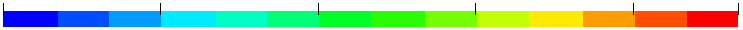
\includegraphics[width=0.26\textwidth]{\myImages/res/k_scale.png}};
	% 	% \node [name = k, anchor = east,at={(osak.north west)},yshift=-0.1cm,xshift=-0.1cm] {\scriptsize{$k$ [-]}};
	% 	% \node [name = psi0, anchor = south,at={(osak.north)},yshift=-0.2cm,xshift=-1.49cm] {\scriptsize{0.00}};
	% 	% \node [name = psi0, anchor = west,at={(psi0.east)},xshift=-0.085cm] {\scriptsize{0.06}};
	% 	% \node [name = psi0, anchor = west,at={(psi0.east)},xshift=-0.08cm] {\scriptsize{0.12}};
	% 	% \node [name = psi0, anchor = west,at={(psi0.east)},xshift=-0.08cm] {\scriptsize{0.18}};
	% 	% \node [name = psi0, anchor = west,at={(psi0.east)},xshift=-0.15cm] {\scriptsize{0.24}};
	% 	% \node [name = psi0, anchor = west,at={(psi0.east)},xshift=-0.2cm] {\scriptsize{0.28}};
	% 	% \node [name = psi0, anchor = west,at={(psi0.east)},xshift=0.06cm] {\scriptsize{}};
	% 	% \node [name = psi0, anchor = west,at={(psi0.east)},xshift=0.06cm] {\scriptsize{0.6}};
	% 	% \node [name = psi0, anchor = west,at={(psi0.east)},xshift=0.06cm] {\scriptsize{0.6}};
	% 	% \node [name = psi0, anchor = west,at={(psi0.east)},xshift=0.228cm] {\scriptsize{0.6}};
	% 	% \node [name = psi0, anchor = west,at={(psi0.east)},xshift=0.228cm] {\scriptsize{1.0}};
	% 	% \node [name = psi0, anchor = west,at={(psi0.east)},xshift=0.02cm] {\scriptsize{1.3}};

	\end{tikzpicture}
}
\newcommand{\compModePoMJednaVDva}[8]{
	\begin{tikzpicture}
		\savebox\mygraphic{\includegraphics[trim = 0px 0px 0px 0px,clip,height=0.237\textwidth,width = 0.41\textwidth]{#1}}
		\begin{axis}[
			name = plot1,
			xlabel={$x_r$ [-]},
			ylabel={$y_r$ [-]},
			font = \scriptsize,
			xtick distance=1,ytick distance=1,
			width=\wd\mygraphic,
			height=\ht\mygraphic, %height= 5/3*0.5
			enlargelimits=false,
			scale only axis=true,
			tick align=outside,
			% x label style = {at={(axis cs:3.5,-2.7)}},
			% y label style = {at={(axis cs:-1,0)}},
			ytick pos=left,
			xtick pos=top,
			line width = 1.7pt
			]
			\addplot graphics[xmin=0, xmax=7, ymin=-2, ymax=2,includegraphics={trim = 0px 0px 0px 0px,clip}] {#1};
			\fill [white] (axis cs:0.001,-1.997) rectangle (axis cs:0.5,1.997);
			\fill [black!70](axis cs:0,0) circle [radius=0.5];
			% \draw [black,dashdotted,line width = 1pt] (axis cs:0,0) -- (axis cs:7,0);
			% \node at (axis cs:6.5,1.7) {\scriptsize{PIV}};
			% \node at (axis cs:6.5,-1.7) {\scriptsize{CFD}};
			% \draw [black!70,dashed,line width = 1pt] (axis cs:3.83,2) -- (axis cs:3.83,-2);
			% \node [black!70] at (axis cs:4.1,1.7) {\scriptsize{$\zeta$}};
			% \node  at (axis cs:6.7,0.3) {\scriptsize{$\sigma$}};
			% \fill [black](axis cs:4,0) circle [radius=0.1];
			% \node  at (axis cs:4.2,-0.3) {\scriptsize{p1}};
			% \fill [black](axis cs:4.53,1.15) circle [radius=0.1];
			% \node  at (axis cs:5,1.15) {\scriptsize{p2}};
		\end{axis}


		\node [name = osaUx,anchor = north,at={(plot1.south)},yshift=-0.0cm] {
\includegraphics[width=0.26\textwidth]{\myImages/res/vorZ_scale.png}};
		\node [name = vorZ, anchor = east,at={(osaUx.north west)},yshift=-0.3cm,xshift=0.0cm] {\scriptsize{$\omega_z$ [-]}};
		\node [name = psi0, anchor = south,at={(osaUx.north)},yshift=-0.6cm,xshift=-1.05cm] {\scriptsize{negative}};
		\node [name = psi0, anchor = west,at={(psi0.east)},yshift=-0.0cm,xshift=0.9cm] {\scriptsize{positive}};
		% \node [name = psi0, anchor = west,at={(psi0.east)},xshift=0.22cm] {\scriptsize{0.2}};
		% \node [name = psi0, anchor = west,at={(psi0.east)},xshift=0.228cm] {\scriptsize{0.6}};
		% \node [name = psi0, anchor = west,at={(psi0.east)},xshift=0.228cm] {\scriptsize{1.0}};
		% \node [name = psi0, anchor = west,at={(psi0.east)},xshift=0.02cm] {\scriptsize{1.3}};
		% \node [name = psiM05, anchor = north west,at={(osaPsix.south west)},yshift=0.2cm] {\scriptsize{-0.1 \%}};
		% \node [name = psiM05, anchor = north east,at={(osaPsix.south east)},yshift=0.2cm] {\scriptsize{0.1 \%}};

		\savebox\mygraphic{\includegraphics[trim = 0px 0px 0px 0px,clip,height=0.237\textwidth,width = 0.41\textwidth]{#2}}
		\begin{axis}[
			name = plot2,
			anchor = north east,
			at = {(plot1.south east)},
			yshift = -0.6cm,
			% xlabel={$x_r$ [-]},
			ylabel={$y_r$ [-]},
			% x label style = {at={(axis cs:3.5,-2.7)}},
			% y label style = {at={(axis cs:7.8,0)}},
			font = \scriptsize,
			xtick distance=1,ytick distance=1,
			width=\wd\mygraphic,
			height=\ht\mygraphic, %height= 5/3*0.5
			enlargelimits=false,
			scale only axis=true,
			ytick pos=left,
			% xtick pos=bottom,
			xticklabels={,,}
			tick align=outside,
			line width = 1.7pt
			]
			\addplot graphics[xmin=0, xmax=7, ymin=-2, ymax=2,includegraphics={trim = 0px 0px 0px 0px,clip}] {#2};
			\fill [white] (axis cs:0.001,-1.997) rectangle (axis cs:0.5,1.997);
			\fill [black!70](axis cs:0,0) circle [radius=0.5];
			% \draw [black,dashdotted,line width = 1.0pt] (axis cs:0,0) -- (axis cs:7,0);
			% \node  at (axis cs:6.7,0.3) {\scriptsize{$\sigma$}};
			% \node [color=black] at (axis cs:6.5,1.7) {\scriptsize{CFD}};
			% \node [color=white] at (axis cs:6.5,-1.7) {\scriptsize{CFD}};
		\end{axis}

		\begin{axis}[
			width=0.41\textwidth,
			% width=0.37\textwidth,
			height = 0.3\textwidth,
			scale only axis,
			name=plot3,
			anchor = north west,
			% xshift=0.3cm,
			yshift=-0.3cm,
			at = {(plot2.south west)},
			xlabel=frequency (Hz),
			tick align=outside,
			ylabel=S.P (a.u),
			ymode=log,
			xmode=log,
			ymax = 200,
			xmin = 1,
			ymin = 1e-2,
			xmax=1e3,
			xtick pos=bottom,
			% ytick pos=right,
			ytick pos=left,
			font=\scriptsize,
			mark size=4pt,    
			% legend style={at={(axis cs:1.5,2e-1)},anchor=north west},
			legend style={anchor=south west},
			legend pos=south west,
			smooth,
			% xtick pos=top,
			line width = 0.85pt,
		]
		\addplot [color = blue,mark =none]table [col sep=comma,y expr=(\thisrow{etaU}/10)^2,x=t]{#3};
		\addlegendentry{PIV}
		\addplot [color = green!70!black,mark =none,each nth point=1]table [col sep=comma,y expr=(\thisrow{etaU}/10)^2,x=t]{#4};
		\addlegendentry{CFD}
		\addplot [color=red,mark=none] coordinates {
			(213,13.16337723958297)
			(1e3,0.9999999999999994 )
		};
		\addlegendentry{Kolm.}
		\addplot [color=black,mark=none,solid] coordinates {
			(71, 1e-4)
			(71, 1e3)
		};
		\addplot [color=black,mark=none,dashed] coordinates {
			(142, 1e-4)
			(142, 1e3)
		};
		\addplot [color=black,mark=none,dashdotted] coordinates {
			(213, 1e-4)
			(213, 1e3)
		};
		\node[above left,anchor=east,black] at (axis cs:71,3e-2) {$f_{1}$};
		\node[above left,anchor=east,black] at (axis cs:162,3e-2) {$f_{2}$};
		\node[above right,anchor=west,black] at (axis cs:213,3e-2) {$f_{3}$};
	\end{axis}
	% \end{tikzpicture}
	% \begin{tikzpicture}
		\savebox\mygraphic{\includegraphics[trim = 0px 0px 0px 0px,clip,height=0.237\textwidth,width = 0.334\textwidth]{#5}}
		\begin{axis}[
			name = plot4,
			at={(plot1.north east)},
			anchor=north west,
			xshift=0.2cm,
			xlabel={$z_r$ [-]},
			ylabel={$y_r$ [-]},
			font = \scriptsize,
			xtick distance=1,ytick distance=1,
			width=\wd\mygraphic,
			height=\ht\mygraphic, %height= 5/3*0.5
			enlargelimits=false,
			scale only axis=true,
			tick align=outside,
			% x label style = {at={(axis cs:3.5,-2.7)}},
			% y label style = {at={(axis cs:-1,0)}},
			ytick pos=right,
			xtick pos=top,
			line width = 1.7pt
			]
			\addplot graphics[xmin=-3, xmax=3, ymin=-2, ymax=2,includegraphics={trim = 0px 0px 0px 0px,clip}] {#5};
			% \fill [white] (axis cs:0.001,-1.997) rectangle (axis cs:0.5,1.997);
			% \fill [black!70](axis cs:0,0) circle [radius=0.5];
			% \draw [black,dashdotted,line width = 1pt] (axis cs:0,0) -- (axis cs:7,0);
			% \node at (axis cs:2.6,1.7) {\scriptsize{PIV}};
			% \node at (axis cs:6.5,-1.7) {\scriptsize{CFD}};
			% \draw [black!70,dashed,line width = 1pt] (axis cs:3.83,2) -- (axis cs:3.83,-2);
			% \node [black!70] at (axis cs:4.1,1.7) {\scriptsize{$\zeta$}};
			% \node  at (axis cs:6.7,0.3) {\scriptsize{$\sigma$}};
			% \fill [black](axis cs:4,0) circle [radius=0.1];
			% \node  at (axis cs:4.2,-0.3) {\scriptsize{p1}};
			% \fill [black](axis cs:4.53,1.15) circle [radius=0.1];
			% \node  at (axis cs:5,1.15) {\scriptsize{p2}};
		\end{axis}


		\node [name = osaUx,anchor = north east,at={(plot4.south east)},yshift=-0.0cm] {
\includegraphics[width=0.26\textwidth]{\myImages/res/vorZ_scale.png}};
		\node [name = vorZ, anchor = east,at={(osaUx.north west)},yshift=-0.3cm,xshift=0.0cm] {\scriptsize{$\psi_{1,x}$ [-]}};
		\node [name = psi0, anchor = south,at={(osaUx.north)},yshift=-0.6cm,xshift=-1.05cm] {\scriptsize{negative}};
		\node [name = psi0, anchor = west,at={(psi0.east)},yshift=-0.0cm,xshift=0.9cm] {\scriptsize{positive}};
		% \node [name = psi0, anchor = west,at={(psi0.east)},xshift=0.22cm] {\scriptsize{0.2}};
		% \node [name = psi0, anchor = west,at={(psi0.east)},xshift=0.228cm] {\scriptsize{0.6}};
		% \node [name = psi0, anchor = west,at={(psi0.east)},xshift=0.228cm] {\scriptsize{1.0}};
		% \node [name = psi0, anchor = west,at={(psi0.east)},xshift=0.02cm] {\scriptsize{1.3}};
		% \node [name = psiM05, anchor = north west,at={(osaPsix.south west)},yshift=0.2cm] {\scriptsize{-0.1 \%}};
		% \node [name = psiM05, anchor = north east,at={(osaPsix.south east)},yshift=0.2cm] {\scriptsize{0.1 \%}};

		\savebox\mygraphic{\includegraphics[trim = 0px 0px 0px 0px,clip,height=0.237\textwidth,width = 0.334\textwidth]{#6}}
		\begin{axis}[
			name = plot5,
			anchor = north east,
			at = {(plot4.south east)},
			yshift = -0.6cm,
			% xlabel={$z_r$ [-]},
			ylabel={$y_r$ [-]},
			% x label style = {at={(axis cs:3.5,-2.7)}},
			% y label style = {at={(axis cs:7.8,0)}},
			font = \scriptsize,
			xtick distance=1,ytick distance=1,
			width=\wd\mygraphic,
			height=\ht\mygraphic, %height= 5/3*0.5
			enlargelimits=false,
			scale only axis=true,
			ytick pos=right,
			xticklabels={,,}
			% xtick pos=bottom,
			tick align=outside,
			line width = 1.7pt
			]
			\addplot graphics[xmin=-3, xmax=3, ymin=-2, ymax=2,includegraphics={trim = 0px 0px 0px 0px,clip}] {#6};
			% \fill [white] (axis cs:0.001,-1.997) rectangle (axis cs:0.5,1.997);
			% \fill [black!70](axis cs:0,0) circle [radius=0.5];
			% \draw [black,dashdotted,line width = 1.0pt] (axis cs:0,0) -- (axis cs:7,0);
			% \node  at (axis cs:6.7,0.3) {\scriptsize{$\sigma$}};
			% \node [color=black] at (axis cs:2.6,1.7) {\scriptsize{CFD}};
			% \node [color=white] at (axis cs:6.5,-1.7) {\scriptsize{CFD}};
		\end{axis}

		\begin{axis}[
			width=0.334\textwidth,
			height = 0.3\textwidth,
			scale only axis,
			name=plot6,
			anchor = north west,
			yshift=-0.3cm,
			at = {(plot5.south west)},
			xlabel=frequency (Hz),
			tick align=outside,
			ylabel=S.P (a.u),
			ymode=log,
			xmode=log,
			ymax = 200,
			xmin = 1,
			ymin = 1e-2,
			xmax=1e3,
			ytick pos=right,
			font=\scriptsize,
			mark size=4pt,   
			legend style={anchor=south west},
			legend pos=south west, 
			% legend style={at={(axis cs:1.5,2e-1)},anchor=north west},
			smooth,
			% xtick pos=top,
			xtick pos=bottom,
			line width = 0.85pt,
		]
		\addplot [color = blue,mark =none]table [col sep=comma,y expr=(\thisrow{etaU}),x=t]{#7};
		\addlegendentry{PIV}
		\addplot [color = green!70!black,mark =none,each nth point=1]table [col sep=comma,y expr=(\thisrow{etaU}),x=t]{#8};
		\addlegendentry{CFD}
		\addplot [color=red,mark=none] coordinates {
			(213,13.16337723958297)
			(1e3,0.9999999999999994 )
		};
		\addlegendentry{Kolm.}
		\addplot [color=black,mark=none,solid] coordinates {
			(71, 1e-4)
			(71, 1e3)
		};
		\addplot [color=black,mark=none,dashed] coordinates {
			(142, 1e-4)
			(142, 1e3)
		};
		\addplot [color=black,mark=none,dashdotted] coordinates {
			(213, 1e-4)
			(213, 1e3)
		};
		\node[above left,anchor=east,black] at (axis cs:71,3e-2) {$f_{1}$};
		\node[above left,anchor=east,black] at (axis cs:162,3e-2) {$f_{2}$};
		\node[above right,anchor=west,black] at (axis cs:213,3e-2) {$f_{3}$};
	\end{axis}
	\node [color=black,anchor=north east,at={(plot1.north east)}] {\scriptsize{PIV}};
	\node [color=black,anchor=north east,at={(plot2.north east)}] {\scriptsize{CFD}};
	\node [color=black,anchor=north east,at={(plot4.north east)}] {\scriptsize{PIV}};
	\node [color=black,anchor=north east,at={(plot5.north east)}] {\scriptsize{CFD}};

	% 	% \node [name = osak,anchor = south east,at={(plot2.south east)},yshift=-0.7cm,xshift=-0.1cm] {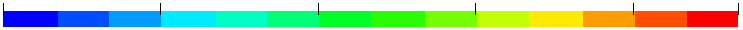
\includegraphics[width=0.26\textwidth]{\myImages/res/k_scale.png}};
	% 	% \node [name = k, anchor = east,at={(osak.north west)},yshift=-0.1cm,xshift=-0.1cm] {\scriptsize{$k$ [-]}};
	% 	% \node [name = psi0, anchor = south,at={(osak.north)},yshift=-0.2cm,xshift=-1.49cm] {\scriptsize{0.00}};
	% 	% \node [name = psi0, anchor = west,at={(psi0.east)},xshift=-0.085cm] {\scriptsize{0.06}};
	% 	% \node [name = psi0, anchor = west,at={(psi0.east)},xshift=-0.08cm] {\scriptsize{0.12}};
	% 	% \node [name = psi0, anchor = west,at={(psi0.east)},xshift=-0.08cm] {\scriptsize{0.18}};
	% 	% \node [name = psi0, anchor = west,at={(psi0.east)},xshift=-0.15cm] {\scriptsize{0.24}};
	% 	% \node [name = psi0, anchor = west,at={(psi0.east)},xshift=-0.2cm] {\scriptsize{0.28}};
	% 	% \node [name = psi0, anchor = west,at={(psi0.east)},xshift=0.06cm] {\scriptsize{}};
	% 	% \node [name = psi0, anchor = west,at={(psi0.east)},xshift=0.06cm] {\scriptsize{0.6}};
	% 	% \node [name = psi0, anchor = west,at={(psi0.east)},xshift=0.06cm] {\scriptsize{0.6}};
	% 	% \node [name = psi0, anchor = west,at={(psi0.east)},xshift=0.228cm] {\scriptsize{0.6}};
	% 	% \node [name = psi0, anchor = west,at={(psi0.east)},xshift=0.228cm] {\scriptsize{1.0}};
	% 	% \node [name = psi0, anchor = west,at={(psi0.east)},xshift=0.02cm] {\scriptsize{1.3}};

	\end{tikzpicture}
}
\newcommand{\compModePoMJednaVTri}[4]{
	\begin{tikzpicture}
		\savebox\mygraphic{\includegraphics[trim = 0px 0px 0px 0px,clip,width = 0.39\textwidth]{#1}}
		\begin{axis}[
			name = plot1,
			xlabel={$x_r$ [-]},
			ylabel={$y_r$ [-]},
			font = \scriptsize,
			xtick distance=1,ytick distance=1,
			width=\wd\mygraphic,
			height=\ht\mygraphic, %height= 5/3*0.5
			enlargelimits=false,
			scale only axis=true,
			tick align=outside,
			% x label style = {at={(axis cs:3.5,-2.7)}},
			% y label style = {at={(axis cs:-1,0)}},
			ytick pos=left,
			xtick pos=top,
			line width = 1.8pt
			]
			\addplot graphics[xmin=0, xmax=7, ymin=-2, ymax=2,includegraphics={trim = 0px 0px 0px 0px,clip}] {#1};
			\fill [white] (axis cs:0.001,-1.997) rectangle (axis cs:0.5,1.997);
			\fill [black!70](axis cs:0,0) circle [radius=0.5];
			% \draw [black,dashdotted,line width = 1pt] (axis cs:0,0) -- (axis cs:7,0);
			% \node at (axis cs:6.5,1.7) {\scriptsize{PIV}};
			% \node at (axis cs:6.5,-1.7) {\scriptsize{CFD}};
			% \draw [black!70,dashed,line width = 1pt] (axis cs:3.83,2) -- (axis cs:3.83,-2);
			% \node [black!70] at (axis cs:4.1,1.7) {\scriptsize{$\zeta$}};
			% \node  at (axis cs:6.7,0.3) {\scriptsize{$\sigma$}};
			% \fill [black](axis cs:4,0) circle [radius=0.1];
			% \node  at (axis cs:4.2,-0.3) {\scriptsize{p1}};
			% \fill [black](axis cs:4.53,1.15) circle [radius=0.1];
			% \node  at (axis cs:5,1.15) {\scriptsize{p2}};
		\end{axis}


		\node [name = osaUx,anchor = north,at={(plot1.south)},yshift=-0.0cm] {
\includegraphics[width=0.26\textwidth]{\myImages/res/vorZ_scale.png}};
		\node [name = vorZ, anchor = east,at={(osaUx.north west)},yshift=-0.3cm,xshift=0.0cm] {\scriptsize{$\omega_z$ [-]}};
		\node [name = psi0, anchor = south,at={(osaUx.north)},yshift=-0.6cm,xshift=-1.05cm] {\scriptsize{negative}};
		\node [name = psi0, anchor = west,at={(psi0.east)},yshift=-0.0cm,xshift=0.9cm] {\scriptsize{positive}};
		% \node [name = psi0, anchor = west,at={(psi0.east)},xshift=0.22cm] {\scriptsize{0.2}};
		% \node [name = psi0, anchor = west,at={(psi0.east)},xshift=0.228cm] {\scriptsize{0.6}};
		% \node [name = psi0, anchor = west,at={(psi0.east)},xshift=0.228cm] {\scriptsize{1.0}};
		% \node [name = psi0, anchor = west,at={(psi0.east)},xshift=0.02cm] {\scriptsize{1.3}};
		% \node [name = psiM05, anchor = north west,at={(osaPsix.south west)},yshift=0.2cm] {\scriptsize{-0.1 \%}};
		% \node [name = psiM05, anchor = north east,at={(osaPsix.south east)},yshift=0.2cm] {\scriptsize{0.1 \%}};

		\savebox\mygraphic{\includegraphics[trim = 0px 0px 0px 0px,clip,width = 0.39\textwidth]{#2}}
		\begin{axis}[
			name = plot2,
			anchor = north west,
			at = {(plot1.north east)},
			xshift = 0.03\textwidth,
			xlabel={$x_r$ [-]},
			ylabel={$y_r$ [-]},
			% x label style = {at={(axis cs:3.5,-2.7)}},
			% y label style = {at={(axis cs:7.8,0)}},
			font = \scriptsize,
			xtick distance=1,ytick distance=1,
			width=\wd\mygraphic,
			height=\ht\mygraphic, %height= 5/3*0.5
			enlargelimits=false,
			scale only axis=true,
			ytick pos=right,
			xtick pos=top,
			% xticklabels={,,}
			tick align=outside,
			line width = 1.8pt
			]
			\addplot graphics[xmin=0, xmax=7, ymin=-2, ymax=2,includegraphics={trim = 0px 0px 0px 0px,clip}] {#2};
			\fill [white] (axis cs:0.001,-1.997) rectangle (axis cs:0.5,1.997);
			\fill [black!70](axis cs:0,0) circle [radius=0.5];
			% \draw [black,dashdotted,line width = 1.0pt] (axis cs:0,0) -- (axis cs:7,0);
			% \node  at (axis cs:6.7,0.3) {\scriptsize{$\sigma$}};
			% \node [color=black] at (axis cs:6.5,1.7) {\scriptsize{CFD}};
			% \node [color=white] at (axis cs:6.5,-1.7) {\scriptsize{CFD}};
		\end{axis}

		\begin{axis}[
			width=0.39\textwidth,
			% width=0.37\textwidth,
			height = 0.28\textwidth,
			scale only axis,
			name=plot3,
			anchor = north west,
			% xshift=0.3cm,
			yshift=-0.4cm,
			at = {(plot2.south west)},
			xlabel=frequency (Hz),
			tick align=outside,
			ylabel=S.P (a.u),
			ymode=log,
			xmode=log,
			ymax = 200,
			xmin = 1,
			ymin = 1e-2,
			xmax=1e3,
			xtick pos=bottom,
			ytick pos=right,
			% ytick pos=left,
			font=\scriptsize,
			mark size=4pt,    
			% legend style={at={(axis cs:1.5,2e-1)},anchor=north west},
			legend style={anchor=south west},
			legend pos=south west,
			smooth,
			% xtick pos=top,
			line width = 0.9pt,
		]
		\addplot [color = blue,mark =none]table [col sep=comma,y expr=(\thisrow{etaU}),x=t]{#3};
		\addlegendentry{PIV}
		\addplot [color = green!70!black,mark =none,each nth point=1]table [col sep=comma,y expr=(\thisrow{etaU}),x=t]{#4};
		\addlegendentry{CFD}
		\addplot [color=red,mark=none] coordinates {
			(213,13.16337723958297)
			(1e3,0.9999999999999994 )
		};
		\addlegendentry{Kolm.}
		\addplot [color=black,mark=none,solid] coordinates {
			(71, 1e-4)
			(71, 1e3)
		};
		\addplot [color=black,mark=none,dashed] coordinates {
			(142, 1e-4)
			(142, 1e3)
		};
		\addplot [color=black,mark=none,dashdotted] coordinates {
			(213, 1e-4)
			(213, 1e3)
		};
		\node[above left,anchor=east,black] at (axis cs:71,3e-2) {$f_{1}$};
		\node[above left,anchor=east,black] at (axis cs:162,3e-2) {$f_{2}$};
		\node[above right,anchor=west,black] at (axis cs:213,3e-2) {$f_{3}$};
	\end{axis}
\end{tikzpicture}
}

\newcommand{\compModePoMDva}[4]{
	\begin{tikzpicture}
		\savebox\mygraphic{\includegraphics[trim = 0px 0px 0px 0px,clip,width = 0.39\textwidth]{#1}}
		\begin{axis}[
			name = plot1,
			xlabel={$z_r$ [--]},
			ylabel={$y_r$ [--]},
			font = \scriptsize,
			xtick distance=1,ytick distance=1,
			width=\wd\mygraphic,
			height=\ht\mygraphic, %height= 5/3*0.5
			enlargelimits=false,
			scale only axis=true,
			tick align=outside,
			% x label style = {at={(axis cs:3.5,-2.7)}},
			% y label style = {at={(axis cs:-1,0)}},
			ytick pos=left,
			% xticklabels=\empty,
			xtick pos=top,
			line width = 1.7pt
			]
			\addplot graphics[xmin=-3, xmax=3, ymin=-2, ymax=2,includegraphics={trim = 0px 0px 0px 0px,clip}] {#1};
			% \fill [white] (axis cs:0.001,-1.997) rectangle (axis cs:0.5,1.997);
			% \fill [black!70](axis cs:0,0) circle [radius=0.5];
			% \draw [black,dashdotted,line width = 1pt] (axis cs:0,0) -- (axis cs:7,0);
			\node at (axis cs:2.6,1.7) {\scriptsize{PIV}};
			% \node at (axis cs:6.5,-1.7) {\scriptsize{CFD}};
			% \draw [black!70,dashed,line width = 1pt] (axis cs:3.83,2) -- (axis cs:3.83,-2);
			% \node [black!70] at (axis cs:4.1,1.7) {\scriptsize{$\zeta$}};
			% \node  at (axis cs:6.7,0.3) {\scriptsize{$\sigma$}};
			% \fill [black](axis cs:4,0) circle [radius=0.1];
			% \node  at (axis cs:4.2,-0.3) {\scriptsize{p1}};
			% \fill [black](axis cs:4.53,1.15) circle [radius=0.1];
			% \node  at (axis cs:5,1.15) {\scriptsize{p2}};
		\end{axis}


		\node [name = osaUx,anchor = south east,at={(plot1.south east)},yshift=-0.35cm] {
\includegraphics[width=0.3\textwidth]{\myImages/res/vorZ_scale.png}};
		\node [name = vorZ, anchor = east,at={(osaUx.north west)},yshift=-0.3cm,xshift=0.0cm] {\scriptsize{$\psi_x$ [--]}};
		\node [name = psi0, anchor = south,at={(osaUx.north)},yshift=-0.6cm,xshift=-1.3cm] {\scriptsize{negative}};
		\node [name = psi0, anchor = west,at={(psi0.east)},yshift=-0.0cm,xshift=1.4cm] {\scriptsize{positive}};
		% \node [name = psi0, anchor = west,at={(psi0.east)},xshift=0.22cm] {\scriptsize{0.2}};
		% \node [name = psi0, anchor = west,at={(psi0.east)},xshift=0.228cm] {\scriptsize{0.6}};
		% \node [name = psi0, anchor = west,at={(psi0.east)},xshift=0.228cm] {\scriptsize{1.0}};
		% \node [name = psi0, anchor = west,at={(psi0.east)},xshift=0.02cm] {\scriptsize{1.3}};
		% \node [name = psiM05, anchor = north west,at={(osaPsix.south west)},yshift=0.2cm] {\scriptsize{-0.1 \%}};
		% \node [name = psiM05, anchor = north east,at={(osaPsix.south east)},yshift=0.2cm] {\scriptsize{0.1 \%}};

		\savebox\mygraphic{\includegraphics[trim = 0px 0px 0px 0px,clip,width = 0.39\textwidth]{#2}}
		\begin{axis}[
			name = plot2,
			anchor = north east,
			at = {(plot1.south east)},
			yshift = -0.65cm,
			% xlabel={$z_r$ [--]},
			ylabel={$y_r$ [--]},
			% x label style = {at={(axis cs:3.5,-2.7)}},
			% y label style = {at={(axis cs:7.8,0)}},
			font = \scriptsize,
			xtick distance=1,ytick distance=1,
			width=\wd\mygraphic,
			height=\ht\mygraphic, %height= 5/3*0.5
			enlargelimits=false,
			scale only axis=true,
			xticklabels=\empty,
			ytick pos=left,
			xtick pos=bottom,
			tick align=outside,
			line width = 0.85pt
			]
			\addplot graphics[xmin=-3, xmax=3, ymin=-2, ymax=2,includegraphics={trim = 0px 0px 0px 0px,clip}] {#2};
			% \fill [white] (axis cs:0.001,-1.997) rectangle (axis cs:0.5,1.997);
			% \fill [black!70](axis cs:0,0) circle [radius=0.5];
			% \draw [black,dashdotted,line width = 1.0pt] (axis cs:0,0) -- (axis cs:7,0);
			% \node  at (axis cs:6.7,0.3) {\scriptsize{$\sigma$}};
			\node [color=black] at (axis cs:2.6,1.7) {\scriptsize{CFD}};
			% \node [color=white] at (axis cs:6.5,-1.7) {\scriptsize{CFD}};
		\end{axis}
		\node [name=a, anchor=north west, at={(plot1.north west)}] {\scriptsize{a)}};
		\node [name=b, anchor=north west, at={(plot2.north west)}] {\scriptsize{b)}};

		\begin{axis}[
			width=0.37\textwidth,
			height = 0.59\textwidth,
			scale only axis,
			name=plot3,
			anchor = north west,
			xshift=0.3cm,
			at = {(plot1.north east)},
			xlabel={$f$ [Hz]},
			ylabel={$E$ [a.u]},
			tick align=outside,
			% ylabel=S.P (a.u),
			ymode=log,
			xmode=log,
			ymax = 200,
			xmin = 1,
			ymin = 1e-5,
			% ymax = 1e4,
			% ymax = 1e-3,
			xmax=1e3,
			ytick pos=right,
			font=\scriptsize,
			mark size=4pt,    
			% legend style={at={(axis cs:1.5,2e-1)},anchor=north west},
			legend style={anchor=south west},
			legend pos=south west,
			smooth,
			xtick pos=top,
			line width = 0.85pt,
		]
		\addplot [color = blue,mark =none]table [col sep=comma,y expr=(\thisrow{etaU}/10)^2,x=t]{#3};
		\addlegendentry{PIV}
		\addplot [color = green!70!black,mark =none,each nth point=1]table [col sep=comma,y expr=(\thisrow{etaU}/10)^2,x=t]{#4};
		\addlegendentry{CFD}
		% \addplot [color=red,mark=none] coordinates {
		% 	(213,13.16337723958297)
		% 	(1e3,0.9999999999999994 )
		% };
		% \addlegendentry{Kolm.}
		% \addplot [color=black,mark=none,solid] coordinates {
		% 	(71, 1e-4)
		% 	(71, 1e3)
		% };
		% \addplot [color=black,mark=none,dashed] coordinates {
		% 	(142, 1e-4)
		% 	(142, 1e3)
		% };
		% \addplot [color=black,mark=none,dashdotted] coordinates {
		% 	(213, 1e-4)
		% 	(213, 1e3)
		% };
		\addplot [color=red,mark=none] coordinates {
			(71,26.282891182634373)
			(333,2 )
		};
		\addlegendentry{Kolm.}
		\addplot [color=orange,mark=none] coordinates {
			(333,2)
			(1e3,0.07385207399999995)
		};
		\addlegendentry{Kraich.}
		\addplot [color=black,mark=none,solid] coordinates {
			(71, 1e-5)
			(71, 1e3)
		};
		\addplot [color=black,mark=none,dashed] coordinates {
			(142, 1e-5)
			(142, 1e3)
		};
		\addplot [color=black,mark=none,dashdotted] coordinates {
			(213, 1e-5)
			(213, 1e3)
		};
		\node[above left,anchor=east,black] at (axis cs:71,3e-5) {$f_{1}$};
		\node[above left,anchor=east,black] at (axis cs:162,3e-5) {$f_{2}$};
		\node[above right,anchor=west,black] at (axis cs:213,3e-5) {$f_{3}$};
		% \node[above left,anchor=east,black] at (axis cs:71,3e-2) {$f_{1}$};
		% \node[above left,anchor=east,black] at (axis cs:162,3e-2) {$f_{2}$};
		% \node[above right,anchor=west,black] at (axis cs:213,3e-2) {$f_{3}$};
	\end{axis}

	\node [name=c, anchor=north west, at={(plot3.north west)}] {\scriptsize{c)}};

	% 	% \node [name = osak,anchor = south east,at={(plot2.south east)},yshift=-0.7cm,xshift=-0.1cm] {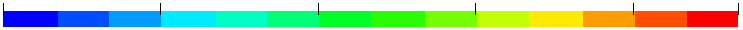
\includegraphics[width=0.26\textwidth]{\myImages/res/k_scale.png}};
	% 	% \node [name = k, anchor = east,at={(osak.north west)},yshift=-0.1cm,xshift=-0.1cm] {\scriptsize{$k$ [-]}};
	% 	% \node [name = psi0, anchor = south,at={(osak.north)},yshift=-0.2cm,xshift=-1.49cm] {\scriptsize{0.00}};
	% 	% \node [name = psi0, anchor = west,at={(psi0.east)},xshift=-0.085cm] {\scriptsize{0.06}};
	% 	% \node [name = psi0, anchor = west,at={(psi0.east)},xshift=-0.08cm] {\scriptsize{0.12}};
	% 	% \node [name = psi0, anchor = west,at={(psi0.east)},xshift=-0.08cm] {\scriptsize{0.18}};
	% 	% \node [name = psi0, anchor = west,at={(psi0.east)},xshift=-0.15cm] {\scriptsize{0.24}};
	% 	% \node [name = psi0, anchor = west,at={(psi0.east)},xshift=-0.2cm] {\scriptsize{0.28}};
	% 	% \node [name = psi0, anchor = west,at={(psi0.east)},xshift=0.06cm] {\scriptsize{}};
	% 	% \node [name = psi0, anchor = west,at={(psi0.east)},xshift=0.06cm] {\scriptsize{0.6}};
	% 	% \node [name = psi0, anchor = west,at={(psi0.east)},xshift=0.06cm] {\scriptsize{0.6}};
	% 	% \node [name = psi0, anchor = west,at={(psi0.east)},xshift=0.228cm] {\scriptsize{0.6}};
	% 	% \node [name = psi0, anchor = west,at={(psi0.east)},xshift=0.228cm] {\scriptsize{1.0}};
	% 	% \node [name = psi0, anchor = west,at={(psi0.east)},xshift=0.02cm] {\scriptsize{1.3}};

	\end{tikzpicture}
}
\newcommand{\compModeTriD}[3]{
	\begin{tikzpicture}
		% \node [name = left,anchor = north,yshift=-0.0cm] {\includegraphics[width=1\textwidth]{#1}};
		\node [name = left,anchor = north,yshift=-0.0cm] {\includegraphics[width=0.94\textwidth]{#1}};
		\node [name = a, anchor=north west,at={(left.north west)}] {\scriptsize{a)}};
-		\node [name = POM1, color=red, anchor = south,at={(left.north)},yshift=-0.07\textwidth,xshift=-0.15\textwidth,rotate=6] {{PoM1}};
		\node [name = POM1, color=green, anchor = south,at={(left.north)},yshift=-0.04\textwidth,xshift=-0.0\textwidth,rotate=-23] {{PoM2}};
		% \node [rotate = 90,name = osaUx,anchor = north,at={(left.west)},xshift=-0.cm] {
\includegraphics[width=0.5\textwidth]{\myImages/res/vorZ_scale.png}};
		\node [rotate = 90,name = osaUx,anchor = north west,at={(left.south west)},yshift=0.5cm] {
\includegraphics[width=0.4\textwidth]{\myImages/res/vorZ_scale.png}};
		\node [name = vorZ, anchor = west,at={(osaUx.south)},yshift=0.15cm,xshift=-0.0cm] {\scriptsize{$\omega_z$ [--]}};
		% \node [name = vorZ, anchor = west,at={(osaUx.south)},yshift=0.15cm,xshift=-0.cm] {\scriptsize{$\omega_z$ [--]}};
		\node [rotate = 90,name = psi0, anchor = north west,at={(osaUx.south west)},yshift=0.15cm,xshift=0cm] {\scriptsize{negative}};
		\node [rotate = 90,name = psi0, anchor = north east,at={(osaUx.south east)},yshift=0.15cm,xshift=0cm] {\scriptsize{positive}};

		\savebox\mygraphic{\includegraphics[trim = 0px 0px 0px 0px,clip,width = 0.39\textwidth]{#2}}
		\begin{axis}[
			name = plot1,
			xlabel={$x_r$ [--]},
			ylabel={$y_r$ [--]},
			font = \scriptsize,
			anchor = north west,
			at = {(left.south west)},
			yshift=-0.2cm,
			xshift=0.9cm,
			xtick distance=1,ytick distance=1,
			width=\wd\mygraphic,
			height = 0.225\textwidth,, %height= 5/3*0.5
			enlargelimits=false,
			scale only axis=true,
			tick align=outside,
			% x label style = {at={(axis cs:3.5,-2.7)}},
			% y label style = {at={(axis cs:-1,0)}},
			ytick pos=left,
			% xtick pos=top,
			xtick pos=bottom,
			line width = 1.7pt,
			% ytick={100,1,0.01,0.0001},
			]
			\addplot graphics[xmin=0, xmax=7, ymin=-2, ymax=2,includegraphics={trim = 0px 0px 0px 0px,clip}] {#2};
			\fill [white] (axis cs:0.001,-1.997) rectangle (axis cs:0.5,1.997);
			\fill [black!70](axis cs:0,0) circle [radius=0.5];
			% \draw [black,dashdotted,line width = 1pt] (axis cs:0,0) -- (axis cs:7,0);
			
			% \node at (axis cs:6.5,-1.7) {\scriptsize{CFD}};
			% \draw [black!70,dashed,line width = 1pt] (axis cs:3.83,2) -- (axis cs:3.83,-2);
			% \node [black!70,anchor=west] at (axis cs:3.83,1.7) {\scriptsize{PoM2}};
			% \node  at (axis cs:6.7,0.3) {\scriptsize{$\sigma$}};
			% \fill [black](axis cs:4,0) circle [radius=0.1];
			% \node  at (axis cs:4.2,-0.3) {\scriptsize{p1}};
			% \fill [black](axis cs:4.53,1.15) circle [radius=0.1];
			% \node  at (axis cs:5,1.15) {\scriptsize{p2}};
		\end{axis}

		\node[anchor=north east] at (plot1.north east) {\scriptsize{PoM1 3D mode slice}};
		\node[anchor=north west] at (plot1.north west) {\scriptsize{b)}};
		
		\begin{axis}[
			width=0.37\textwidth,
			height = 0.225\textwidth,
			scale only axis,
			name=plot4,
			anchor = north west ,
			xshift=0.3cm,
			at = {(plot1.north east)},
			% xlabel=frequency (Hz),
			tick align=outside,
			% ylabel=S.P (a.u),
			xlabel={$f$ [Hz]},
			ylabel={$E$ [a.u]},
			ymode=log,
			xmode=log,
			ymax = 200,
			xmin = 1,
			ymin = 1e-5,
			xmax=1e3,
			ytick pos=right,
			font=\scriptsize,
			mark size=4pt,    
			% legend style={at={(axis cs:1.5,2e-1)},anchor=north west},
			legend style={anchor=south west},
			legend pos=south west,
			smooth,
			xtick pos=bottom,
			line width = 0.85pt,
		]
		\addplot [color = blue,mark =none]table [col sep=comma,y expr=(\thisrow{etaU}/10)^2,x=t]{#3};
		\addlegendentry{3D CFD}
		\addplot [color=red,mark=none] coordinates {
			(71,26.282891182634373)
			(333,2 )
		};
		\addlegendentry{Kolm.}
		\addplot [color=orange,mark=none] coordinates {
			(333,2)
			(1e3,0.07385207399999995)
		};
		\addlegendentry{Kraich.}
		\addplot [color=black,mark=none,solid] coordinates {
			(71, 1e-5)
			(71, 1e3)
		};
		\addplot [color=black,mark=none,dashed] coordinates {
			(142, 1e-5)
			(142, 1e3)
		};
		\addplot [color=black,mark=none,dashdotted] coordinates {
			(213, 1e-5)
			(213, 1e3)
		};
		\node[above left,anchor=east,black] at (axis cs:71,3e-5) {$f_{1}$};
		\node[above left,anchor=east,black] at (axis cs:162,3e-5) {$f_{2}$};
		\node[above right,anchor=west,black] at (axis cs:213,3e-5) {$f_{3}$};
		\end{axis}
		\node[anchor=north west] at (plot4.north west) {\scriptsize{c)}};
	\end{tikzpicture}
}


\newcommand{\reconTwo}[2]{
	\begin{tikzpicture}
		\savebox\mygraphic{\includegraphics[trim = 0px 0px 0px 0px,clip,width = 0.39\textwidth]{#1}}
		\begin{axis}[
			name = plot1,
			xlabel={$x_r$ [--]},
			ylabel={$y_r$ [--]},
			font = \scriptsize,
			anchor = north west,
			%~ at = {(left.south west)},
			yshift=-0.2cm,
			xshift=0.9cm,
			xtick distance=1,ytick distance=1,
			width=\wd\mygraphic,
			height = 0.225\textwidth,, %height= 5/3*0.5
			enlargelimits=false,
			scale only axis=true,
			tick align=outside,
			% x label style = {at={(axis cs:3.5,-2.7)}},
			% y label style = {at={(axis cs:-1,0)}},
			ytick pos=left,
			% xtick pos=top,
			xtick pos=bottom,
			line width = 1.7pt,
			% ytick={100,1,0.01,0.0001},
			]
			\addplot graphics[xmin=0, xmax=7, ymin=-2, ymax=2,includegraphics={trim = 0px 0px 0px 0px,clip}] {#1};
			\fill [white] (axis cs:0.001,-1.997) rectangle (axis cs:0.5,1.997);
			\fill [black!70](axis cs:0,0) circle [radius=0.5];
            
            \node[anchor=north west] at (rel axis cs:0.01,0.99) {a)};
			% \draw [black,dashdotted,line width = 1pt] (axis cs:0,0) -- (axis cs:7,0);
			
			% \node at (axis cs:6.5,-1.7) {\scriptsize{CFD}};
			% \draw [black!70,dashed,line width = 1pt] (axis cs:3.83,2) -- (axis cs:3.83,-2);
			% \node [black!70,anchor=west] at (axis cs:3.83,1.7) {\scriptsize{PoM2}};
			% \node  at (axis cs:6.7,0.3) {\scriptsize{$\sigma$}};
			% \fill [black](axis cs:4,0) circle [radius=0.1];
			% \node  at (axis cs:4.2,-0.3) {\scriptsize{p1}};
			% \fill [black](axis cs:4.53,1.15) circle [radius=0.1];
			% \node  at (axis cs:5,1.15) {\scriptsize{p2}};
		\end{axis}

		% \node[anchor=north east] at (plot1.north east) {\scriptsize{PoM1 3D mode slice}};
		% \node[anchor=north west] at (plot1.north west) {\scriptsize{b)}};
		
		% \node [name = left,anchor = north,yshift=-0.0cm] {\includegraphics[width=1\textwidth]{#1}};
		\node [at={(plot1.east)},name = left,anchor = west,xshift=0.05\textwidth] {\includegraphics[width=0.5\textwidth]{#2}};
        \node[anchor=south west,font=\scriptsize] at (left.south west) {b)};
		% \node [name = a, anchor=north west,at={(left.north west)}] {\scriptsize{a)}};
% -		\node [name = POM1, color=red, anchor = south,at={(left.north)},yshift=-0.07\textwidth,xshift=-0.15\textwidth,rotate=6] {{PoM1}};
		% \node [name = POM1, color=green, anchor = south,at={(left.north)},yshift=-0.04\textwidth,xshift=-0.0\textwidth,rotate=-23] {{PoM2}};
		\node [name = osaUx,anchor = south west,at={(plot1.north)},yshift=0.1cm] {
\includegraphics[width=0.4\textwidth]{\myImages/res/vorZ_scale.png}};
		% \node [rotate = 90,name = osaUx,anchor = north west,at={(left.south west)},yshift=0.5cm] {
\includegraphics[width=0.4\textwidth]{\myImages/res/vorZ_scale.png}};
		\node [name = vorZ, anchor = east,at={(osaUx.west)},yshift=0.cm,xshift=-0.0cm] {\scriptsize{$\omega_z$ [--]}};
		% \node [name = vorZ, anchor = west,at={(osaUx.south)},yshift=0.15cm,xshift=-0.cm] {\scriptsize{$\omega_z$ [--]}};
		\node [name = psi0, anchor = south west,at={(osaUx.north west)},yshift=-0.18cm,xshift=0cm] {\scriptsize{negative}};
		\node [name = psi0, anchor = south east,at={(osaUx.north east)},yshift=-0.18cm,xshift=0cm] {\scriptsize{positive}};
	\end{tikzpicture}
}
\newcommand{\reconFourDvaD}[4]{
	\begin{tikzpicture}
		\savebox\mygraphic{\includegraphics[trim = 0px 0px 0px 0px,clip,width = 0.39\textwidth]{#1}}
		\begin{axis}[
			name = plot1,
			xlabel={$x_r$ [--]},
			ylabel={$y_r$ [--]},
			font = \scriptsize,
			anchor = north west,
			%~ at = {(left.south west)},
			yshift=-0.2cm,
			xshift=0.9cm,
			xtick distance=1,ytick distance=1,
			width=\wd\mygraphic,
			height = 0.225\textwidth,, %height= 5/3*0.5
			enlargelimits=false,
			scale only axis=true,
			tick align=outside,
			% x label style = {at={(axis cs:3.5,-2.7)}},
			% y label style = {at={(axis cs:-1,0)}},
			ytick pos=left,
			xtick pos=top,
			% xtick pos=bottom,
			line width = 1.7pt,
			% ytick={100,1,0.01,0.0001},
			]
			\addplot graphics[xmin=0, xmax=7, ymin=-2, ymax=2,includegraphics={trim = 0px 0px 0px 0px,clip}] {#1};
			\fill [white] (axis cs:0.001,-1.997) rectangle (axis cs:0.5,1.997);
			\fill [black!70](axis cs:0,0) circle [radius=0.5];
            \node[anchor=north west] at (rel axis cs:0.01,0.99) {a)};
		\end{axis}

		\savebox\mygraphic{\includegraphics[trim = 0px 0px 0px 0px,clip,width = 0.39\textwidth]{#2}}
		\begin{axis}[
			name = plot2,
			xlabel={$x_r$ [--]},
			ylabel={$y_r$ [--]},
			font = \scriptsize,
			anchor = north west,
			at = {(plot1.north east)},
			yshift=-0.0cm,
			xshift=0.2cm,
			xtick distance=1,ytick distance=1,
			width=\wd\mygraphic,
			height = 0.225\textwidth,, %height= 5/3*0.5
			enlargelimits=false,
			scale only axis=true,
			tick align=outside,
			% x label style = {at={(axis cs:3.5,-2.7)}},
			% y label style = {at={(axis cs:-1,0)}},
			ytick pos=right,
			% ytick pos=left,
			xtick pos=top,
			% xtick pos=bottom,
			line width = 1.7pt,
			% ytick={100,1,0.01,0.0001},
			]
			\addplot graphics[xmin=0, xmax=7, ymin=-2, ymax=2,includegraphics={trim = 0px 0px 0px 0px,clip}] {#2};
			\fill [white] (axis cs:0.001,-1.997) rectangle (axis cs:0.5,1.997);
			\fill [black!70](axis cs:0,0) circle [radius=0.5];
            \node[anchor=north west] at (rel axis cs:0.01,0.99) {b)};
		\end{axis}

		\savebox\mygraphic{\includegraphics[trim = 0px 0px 0px 0px,clip,width = 0.39\textwidth]{#3}}
		\begin{axis}[
			name = plot3,
			% xlabel={$x_r$ [--]},
			ylabel={$y_r$ [--]},
			font = \scriptsize,
			anchor = north west,
			at = {(plot1.south west)},
			yshift=-0.2cm,
			% xshift=0.9cm,
			xtick distance=1,ytick distance=1,
			width=\wd\mygraphic,
			height = 0.225\textwidth,, %height= 5/3*0.5
			enlargelimits=false,
			scale only axis=true,
			tick align=outside,
			% x label style = {at={(axis cs:3.5,-2.7)}},
			% y label style = {at={(axis cs:-1,0)}},
			ytick pos=left,
			% xtick pos=top,
			xtick pos=bottom,
			xticklabels=\empty,
			line width = 1.7pt,
			% ytick={100,1,0.01,0.0001},
			]
			\addplot graphics[xmin=0, xmax=7, ymin=-2, ymax=2,includegraphics={trim = 0px 0px 0px 0px,clip}] {#3};
			\fill [white] (axis cs:0.001,-1.997) rectangle (axis cs:0.5,1.997);
			\fill [black!70](axis cs:0,0) circle [radius=0.5];
            \node[anchor=north west] at (rel axis cs:0.01,0.99) {c)};
		\end{axis}
		\node [name = osaUx,anchor = north west,at={(plot3.south)},yshift=-0.15cm] {
\includegraphics[width=0.4\textwidth]{\myImages/res/vorZ_scale.png}};
		% \node [rotate = 90,name = osaUx,anchor = north west,at={(left.south west)},yshift=0.5cm] {
\includegraphics[width=0.4\textwidth]{\myImages/res/vorZ_scale.png}};
		\node [name = vorZ, anchor = east,at={(osaUx.west)},yshift=0.cm,xshift=-0.0cm] {\scriptsize{$\omega_z$ [--]}};
		% \node [name = vorZ, anchor = west,at={(osaUx.south)},yshift=0.15cm,xshift=-0.cm] {\scriptsize{$\omega_z$ [--]}};
		\node [name = psi0, anchor = north west,at={(osaUx.south west)},yshift=0.18cm,xshift=0cm] {\scriptsize{negative}};
		\node [name = psi0, anchor = north east,at={(osaUx.south east)},yshift=0.18cm,xshift=0cm] {\scriptsize{positive}};

		\savebox\mygraphic{\includegraphics[trim = 0px 0px 0px 0px,clip,width = 0.39\textwidth]{#4}}
		\begin{axis}[
			name = plot4,
			% xlabel={$x_r$ [--]},
			ylabel={$y_r$ [--]},
			font = \scriptsize,
			anchor = north west,
			at = {(plot3.north east)},
			% yshift=-0.2cm,
			xshift=0.2cm,
			xtick distance=1,ytick distance=1,
			width=\wd\mygraphic,
			height = 0.225\textwidth,, %height= 5/3*0.5
			enlargelimits=false,
			scale only axis=true,
			xticklabels=\empty,
			tick align=outside,
			% x label style = {at={(axis cs:3.5,-2.7)}},
			% y label style = {at={(axis cs:-1,0)}},
			% ytick pos=left,
			ytick pos=right,
			% xtick pos=top,
			xtick pos=bottom,
			line width = 1.7pt,
			% ytick={100,1,0.01,0.0001},
			]
			\addplot graphics[xmin=0, xmax=7, ymin=-2, ymax=2,includegraphics={trim = 0px 0px 0px 0px,clip}] {#4};
			\fill [white] (axis cs:0.001,-1.997) rectangle (axis cs:0.5,1.997);
			\fill [black!70](axis cs:0,0) circle [radius=0.5];
            \node[anchor=north west] at (rel axis cs:0.01,0.99) {d)};
		\end{axis}
		% \node [at={(plot1.east)},name = left,anchor = west,xshift=0.05\textwidth] {\includegraphics[width=0.5\textwidth]{#2}};
	\end{tikzpicture}
}

\newcommand{\reconFourTriD}[4]{
	\begin{tikzpicture}
		\node [name=plot1] {\includegraphics[width=0.48\textwidth]{#1}};
		\node [at={(plot1.north east)},name = plot2,anchor = north west,xshift=0.2cm] {\includegraphics[width=0.48\textwidth]{#2}};
		\node [at={(plot1.south west)},name = plot3,anchor = north west,yshift=-0.2cm] {\includegraphics[width=0.48\textwidth]{#3}};
		\node [at={(plot3.north east)},name = plot4,anchor = north west,xshift=0.2cm] {\includegraphics[width=0.48\textwidth]{#4}};
		\node [name = osaUx,anchor = south west,at={(plot1.north)},xshift=0.3cm,yshift=0.1cm] {
\includegraphics[width=0.4\textwidth]{\myImages/res/vorZ_scale.png}};
        \node[anchor=south west,font=\scriptsize] at (plot1.south west) {a)};
        \node[anchor=south west,font=\scriptsize] at (plot2.south west) {b)};
        \node[anchor=south west,font=\scriptsize] at (plot3.south west) {c)};
        \node[anchor=south west,font=\scriptsize] at (plot4.south west) {d)};
		% \node [rotate = 90,name = osaUx,anchor = north west,at={(left.south west)},yshift=0.5cm] {
\includegraphics[width=0.4\textwidth]{\myImages/res/vorZ_scale.png}};
		\node [name = vorZ, anchor = east,at={(osaUx.west)},yshift=0.cm,xshift=-0.0cm] {\scriptsize{$\omega_z$ [--]}};
		% \node [name = vorZ, anchor = west,at={(osaUx.south)},yshift=0.15cm,xshift=-0.cm] {\scriptsize{$\omega_z$ [--]}};
		\node [name = psi0, anchor = south west,at={(osaUx.north west)},yshift=-0.18cm,xshift=0cm] {\scriptsize{negative}};
		\node [name = psi0, anchor = south east,at={(osaUx.north east)},yshift=-0.18cm,xshift=0cm] {\scriptsize{positive}};
	\end{tikzpicture}
}



% - math operators
\newcommand{\norm}[1]{\left\lVert#1\right\rVert}
\DeclareMathOperator*{\argmin}{arg\,min}
\DeclareMathOperator*{\argmax}{arg\,max}
\DeclareRobustCommand\myTikzDot{\tikz \node[mark size=2pt,color=black!50!white] at (1ex,2ex) {\pgfuseplotmark{*}};}
\DeclareRobustCommand\myTikzTriangle{\tikz \node[mark size=2pt,color=black] at (1ex,2ex) {\pgfuseplotmark{triangle*}};}

% - math symbols
\newcommand{\OmegaS}{\Omega_{\mathrm{s}}}                               %solid domain
\newcommand{\OmegaF}{\Omega_{\mathrm{f}}}                               %fluid domain
\newcommand{\transp}{\mathrm{T}}
% - flow symbols
\newcommand{\Rey}{\mathrm{Re}}                                          %reynolds number
\newcommand{\Strou}{\mathrm{Sr}}                                        %strouhal number
\newcommand{\Drag}{\mathrm{C_{D}}}                                      %drag coefficient
\newcommand{\Lift}{\mathrm{C_{L}}}                                      %lift coefficient
\newcommand{\filtU}{\overline{\bm{u}}}
\newcommand{\filtP}{\overline{\bm{p}}}
\newcommand{\filtT}{\overline{\bm{\sigma}}}
\newcommand{\sgsT}{\bm{\tau}}
% - units
\newcommand{\mUnit}{[\mathrm{M}]}                                       %mass
\newcommand{\vUnit}{[\mathrm{L\,T^{-1}}]}                               %velocity
\newcommand{\vAngUnit}{[\mathrm{rad\,T^{-1}}]}                          %velocity
\newcommand{\aUnit}{[\mathrm{L\,T^{-2}}]}                               %acceleration
\newcommand{\aAngUnit}{[\mathrm{rad\,T^{-2}}]}                          %acceleration - angular
\newcommand{\lUnit}{[\mathrm{L}]}                                       %length
\newcommand{\lAngUnit}{[\mathrm{rad}]}                                  %unit
\newcommand{\fUnit}{[\mathrm{M\,L\,T^{-2}}]}                            %force
\newcommand{\pUnit}{[\mathrm{M\,L^{-1}T^{-2}}]}                         %pressure
\newcommand{\kPUnit}{[\mathrm{L^{2}T^{-2}}]}                            %kinematic pressure
\newcommand{\volUnit}{[\mathrm{L^{3}}]}                                 %volume
\newcommand{\dUnit}{[\mathrm{M\,L^{3}}]}                                %density
\newcommand{\ndUnit}{[\mathrm{-}]}                                      %dimensionless
\newcommand{\kViscUnit}{[\mathrm{L^{2}T^{-1}}]}                         %kinematic viscosity
% - additional symbols

% - auxiliaries (to be removed before submission)
%~ \newcommand{\noteMI}[1]{\textcolor{red}{#1}} 
%~ \newcommand{\noteTH}[1]{\textcolor{green}{#1}} 
\newcommand{\noteMI}[1]{\textcolor{green}{#1}} 
\newcommand{\noteTH}[1]{\textcolor{red}{#1}} 

\newlength{\auxWidth}
\setlength{\auxWidth}{16.5cm}%


\makeatother
%%%%%%%%%%%%%%%%%%%%%%%%%%%%%%%%%%%%%%%%%%%%%%%%%%%%%%%%%%%%%%%%%%%%%%%%

\hypersetup{
    colorlinks=true,       % false: boxed links; true: colored links
    linkcolor=black,          % color of internal links
    citecolor=black,        % color of links to bibliography
    filecolor=black,      % color of file links
    urlcolor=black,           % color of external links
    allcolors=black
}

\begin{document}

\begin{frontmatter}

\title
{
 Validated mathematical modeling of wake dynamics behind a circular cylinder using Proper Orthogonal Decomposition
}

\address[ITCAS]
{
 Institute of Thermomechanics of the Czech Academy of Sciences,
 Dolej\v{s}kova 5, Prague 182~00, Czech Republic
}

\address[CTU]
{
 Czech Technical University in Prague,
 Department of Technical Mathematics,
 Jugoslávských partyzánů 1580, Prague 160 00, Czech Republic
}

\address[VSCHTDM]
{
 University of~Chemistry and Technology, Prague,
 Department of~Mathematics,
 Technick\'{a}~5, Prague 166~28, Czech Republic
}

% \address[VSCHT]
% {
%  University of~Chemistry and Technology, Prague,
%  Department of~Chemical Engineering,
%  Technick\'{a}~5, Prague 166~28, Czech Republic
% }



\address[ZCU]
{
 University of~West Bohemia, Pilsen,
 Department of Power System Engineering,
 Universitn\'{i}~8, Pilsen 301~00, Czech Republic
}


%% Group authors per affiliation:
\author[ITCAS,CTU]{Tom\'{a}\v{s} Hlavat\'{y}}
\author[ITCAS,VSCHTDM]{Martin Isoz\corref{cor}}
\cortext[cor]{Corresponding author,
tel: \mbox{+420 26605 3441}.}
\ead{isozm@it.cas.cz}
\ead[url]{https://www.it.cas.cz/en/d4/}
\author[ITCAS,ZCU]{V\'{a}clav Uruba}
\author[ITCAS]{Pavel Proch\'{a}zka}


\begin{abstract}
{Turbulent flow in the wake behind a circular cylinder in a cross-flow at Reynolds number of $4815$ was investigated both experimentally, utilizing a time-resolved variant of the Particle Image Velocimetry (PIV) and stereo-PIV methods, and via $k$-$\omega$\textsubscript{SST} Detached-Eddy Simulation (DES) mathematical modeling. The simulated flow statistical properties were validated via a comparison of the time-averaged measured and computed velocity and vorticity fields. To validate the flow dynamical behavior, the agreeement between the measured and computed velocity spectra was evaluated and results of the Proper Orthogonal Decomposition (POD) of experimental and simulated spatio-temporal velocity data were analyzed. All the performed validations have shown an acceptable agreement between the experiment and the simulation enabling a fully 3D POD analysis of the wake flow numerical data.}
\end{abstract}

\begin{keyword}
3D turbulent flow\sep
LES\sep
DES\sep 
proper orthogonal decomposition
\end{keyword}

\end{frontmatter}

\linenumbers

\clearpage
\section{Introduction}
\label{sec:intro}
%The flow in the wake behind a circular cylinder in a cross-flow is one of the canonical cases of fluid mechanics. Thus, extensive amount of information on it may be found from the experimental \citep{kovasznay1949,roshko1953,roshko1955,tritton1959,tyler1931,relf1925,relf1921,norberg1994,wieselsberger1921,lienhard1966,jordan1972,williamson1989,williamson1996,prasad1997}, theoretical \citep{schatzmann1981,saffman1982,crowdy2017,williamson1996} and computational \citep{braza1986,sirisup2004,henderson1995,fiabane2011} point of view. \noteTH{Too many citations here, reduce to the most important.} 
Understanding the flow behind a circular cylinder, or a bluff body in general, poses a great challenge. The complexity of bluff body wakes arises from the fact that they are governed by interactions of three shear layers
\begin{inparaenum}[(i)]
        \item a boundary layer,
        \item a separating free shear layer, and
        \item a wake \citep{williamson1996}. 
\end{inparaenum}

\noteTH{These interactions result in a famous von Karman vortex shedding behind the bluff body occurring over a wide range of the Reynolds numbers. Clear insight into this phenomenon is very important from the engineering point of view as it 
\begin{inparaenum}[(i)]
        \item significantly increases mean drag and lift fluctuations~\cite{chu21}, and
        \item can be used in both passive and active flow controls~\cite{choi08}.
\end{inparaenum}
}

The ongoing developments in numerical methods, available computing power and experimental techniques enable more and more detailed studies of the phenomenon in question. For example, \noteTH{\citet{}} studied... However, modern methods such as particle image velocimetry (PIV) or computational fluid dynamics (CFD) generate vast and complex high-dimensional data. The abundance of raw information on the studied problem provokes the need for a methodology allowing to sort the data in {such} a manner {that} the experimental or numerical results may be interpreted in a way shedding light on the studied problem principles.

One of the purely data-based techniques for flow field analysis is the proper orthogonal decomposition (POD). For a given dataset, POD provides an orthonormal basis that is, in the least squares sense, optimally ordered with respect to the amount of variance in the original data it represents \citep{isoz2019}. Furthermore, if the studied data correspond to the velocity fluctuations, POD optimally captures the flow turbulence kinetic energy ($k$) and the generated basis vectors are ordered by the amount of $k$ they capture \citep{taira2020}. POD was first introduced by \citet{Pearson1901} more than a century ago. However, due to its importance in a variety of fields, it was reinvented multiple times as, e.g., 
\begin{inparaenum}[(i)]
        \item principal component analysis \citep{hoetelling1935,jollife2014} and total least squares estimation in statistics \citep{vanHuffel2013,schaffrin2006,leyang2012},
        \item empirical orthogonal functions in meteorology \citep{lorenzxy}, or
        \item or Karhunen-Loeve decomposition in signal processing \citep{karhunen1946,loeve1946}. 
\end{inparaenum}

Besides being able to effectively identify dominant flow features, POD has been proven to be an effective method for compressing and summarizing large datasets in a way that the most useful information on the physical processes may be extracted \citep{kostas2005,feng2010}. Consequently, POD has been applied to analyze many problems of fluid mechanics, e.g. flow past a backward-facing step \citep{kostas2005,kostas2002}, flow over different bottom-mounted ribs \citep{fraga2021}, flow behind a fixed circular cylinder \citep{venturi2006,ma2000,ma2003,feng2010} or a circular cylinder undergoing vortex-induced vibrations \citep{riches2018}.

\noteTH{Any coupled experimental and numerical studies at similar Re?}
\noteTH{How often is 3D POD analysis of validated CFD DES/LES data?}

In the present paper, we concentrate on the case of the flow in the wake behind a {fixed} circular cylinder in a cross-flow at Reynolds number of $4815$. An experimental and numerical investigations of the problem are coupled in order to enable a detailed study of the flow dynamics via a validated proper orthogonal decomposition analysis of the fully three-dimensional numerical data. The experiment is similar as published in \citep{uruba2020,uruba2020a}, i.e. it is based on the particle image velocimetry (PIV) and designed to bring detailed data on flow dynamics. In particular, the time-resolved PIV and stereo-PIV are used to provide information on flow on selected planes inside the experimental test-section. The simulation corresponds as well as possible to the employed experimental set up. The approach of choice for the turbulence modeling is the $k-\omega$ shear stress transport (SST) detached eddy simulation (DES) model based on the work {of} \citet{strelets2001}. Although the used turbulence model is a hybrid large eddy simulation (LES)-Reynolds-averaged Navier-Stokes (RANS) model, the computational mesh is prepared in a way that the selected modeling approach provides high-resolution data in the zone of interest corresponding to the measured region.

The main contribution of the present work lies in {the} availability of directly comparable experimental and numerical data for both the statistical and dynamic flow properties. First, the simulation is, similarly to \citep{jie2016,gonzalez2019}, validated against the experimental data with respect to
\begin{inparaenum}[(i)]
        \item time-averaged quantities, and
        \item spectra of velocity components at given locations.
\end{inparaenum}
Next, the results of POD analysis of numerical and experimental data on the measured planes were compared to each other. Such a comparison allowed us to validate the predicted coherent flow structures and their energies, leading to {a} validated fully three-dimensional (3D) numerical POD results. Finally, the 3D POD data are used to draw conclusions on the studied flow behavior.
% Note (MI): I think this remains usable even with the small change in the article structure


\section{Problem geometry and experimental setup}
\label{sec:experiments}

\begin{figure}[htbp]
    \centering
    % \begin{tikzpicture}[
    % axPic/.pic={
    %         \draw[->,-triangle 45] (0,0) -- (-0.15,1)  node (ysign) [pos=1,right] {$y$};
    %         \draw[->,-triangle 45] (0,0) -- (0.9,0.27) node (xsign) [pos=1,right] {$x$};
    %         \draw[->,-triangle 45] (0,0) -- (0.6,-0.2) node (zsign) [pos=1,right] {$z$};
    %         \node[font=\scriptsize,xshift=0.4cm]  at (ysign.north) {{(transverse)}};
    %         \node[font=\scriptsize,xshift=0.48cm] at (xsign.south) {{(streamwise)}};
    %         \node[font=\scriptsize,xshift=0.4cm]  at (zsign.south) {{(spanwise)}};
    %      }
    % ]
    %     \node (0,0) (geomFig) {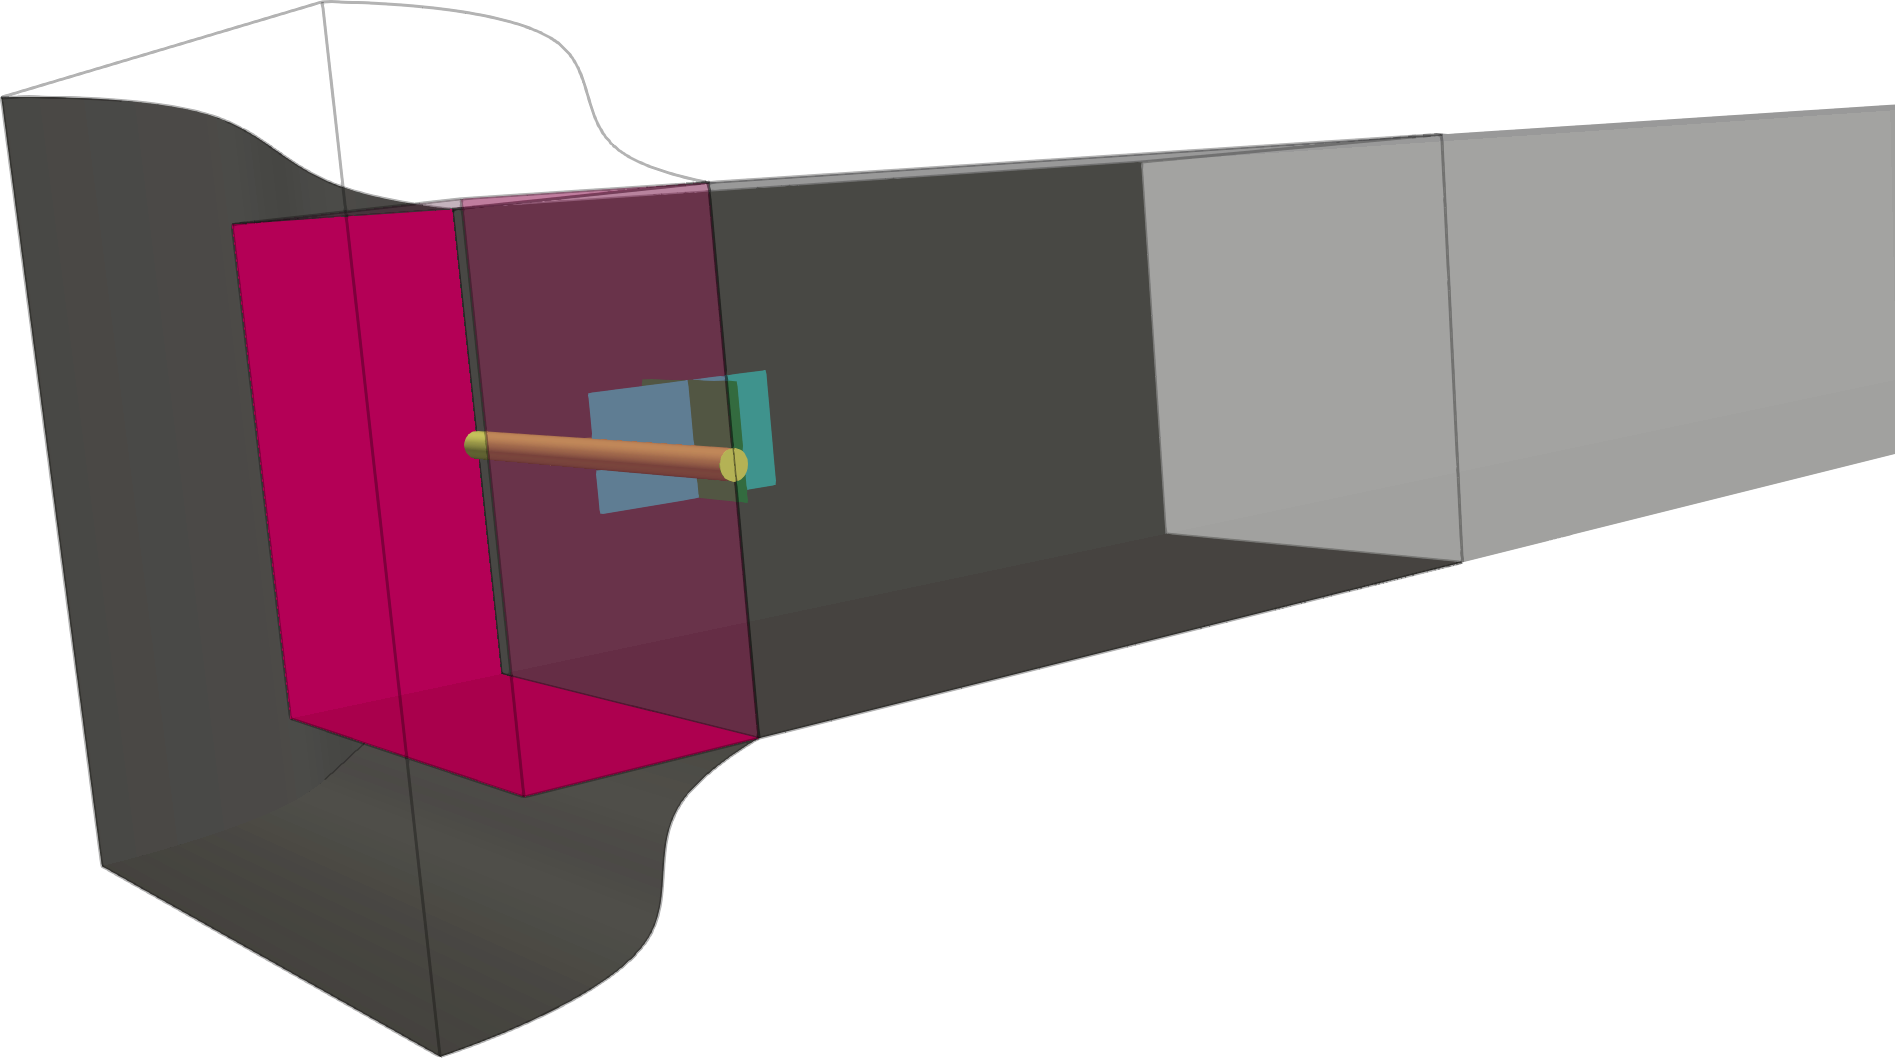
\includegraphics[width=0.9\textwidth]{\myImages/windTunnelFullV2.png}};
    %     \node[anchor=south east] (cylFig) at (geomFig.south east) {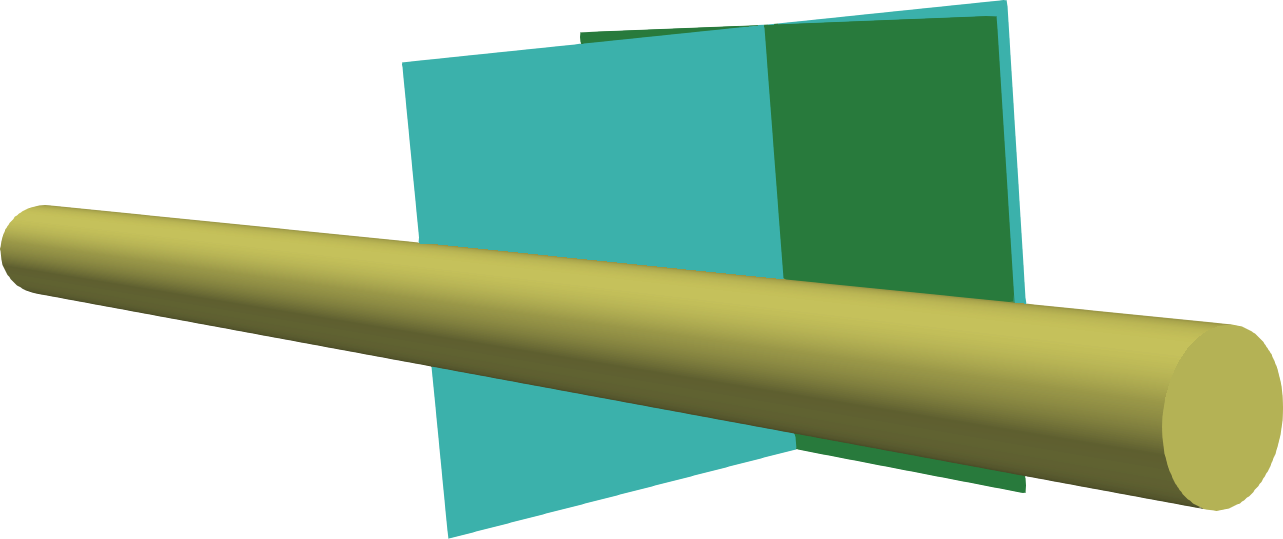
\includegraphics[width=0.45\textwidth]{\myImages/cyllAndPoMsV3.png}};
    %     \node[anchor=north,below left=0.3cm and 1cm] at (geomFig.north) {a)};
    %     \node[anchor=north west,below right=0.3 and 0.3cm] at (cylFig.north west) {b)};
    %     \draw (-1.3,-3) pic[solid] {axPic};
    %     \draw[->,-triangle 45,thick, red!80!black] (-0.5,-2.5) -- (1.1,-2.05) node[pos=0.2,above]{$\bm{u}_{\mathrm{in}}$};
    %     \draw[->,teal!70!white,thick] (1,-1.1) -- (1.7,-1.5) node[pos=0.2,above]{PoM1};
    %     \draw[->,green!70!black,thick] (5,-1.1) -- (4,-1.5) node[pos=0.0,above]{PoM2};
    % \end{tikzpicture}
    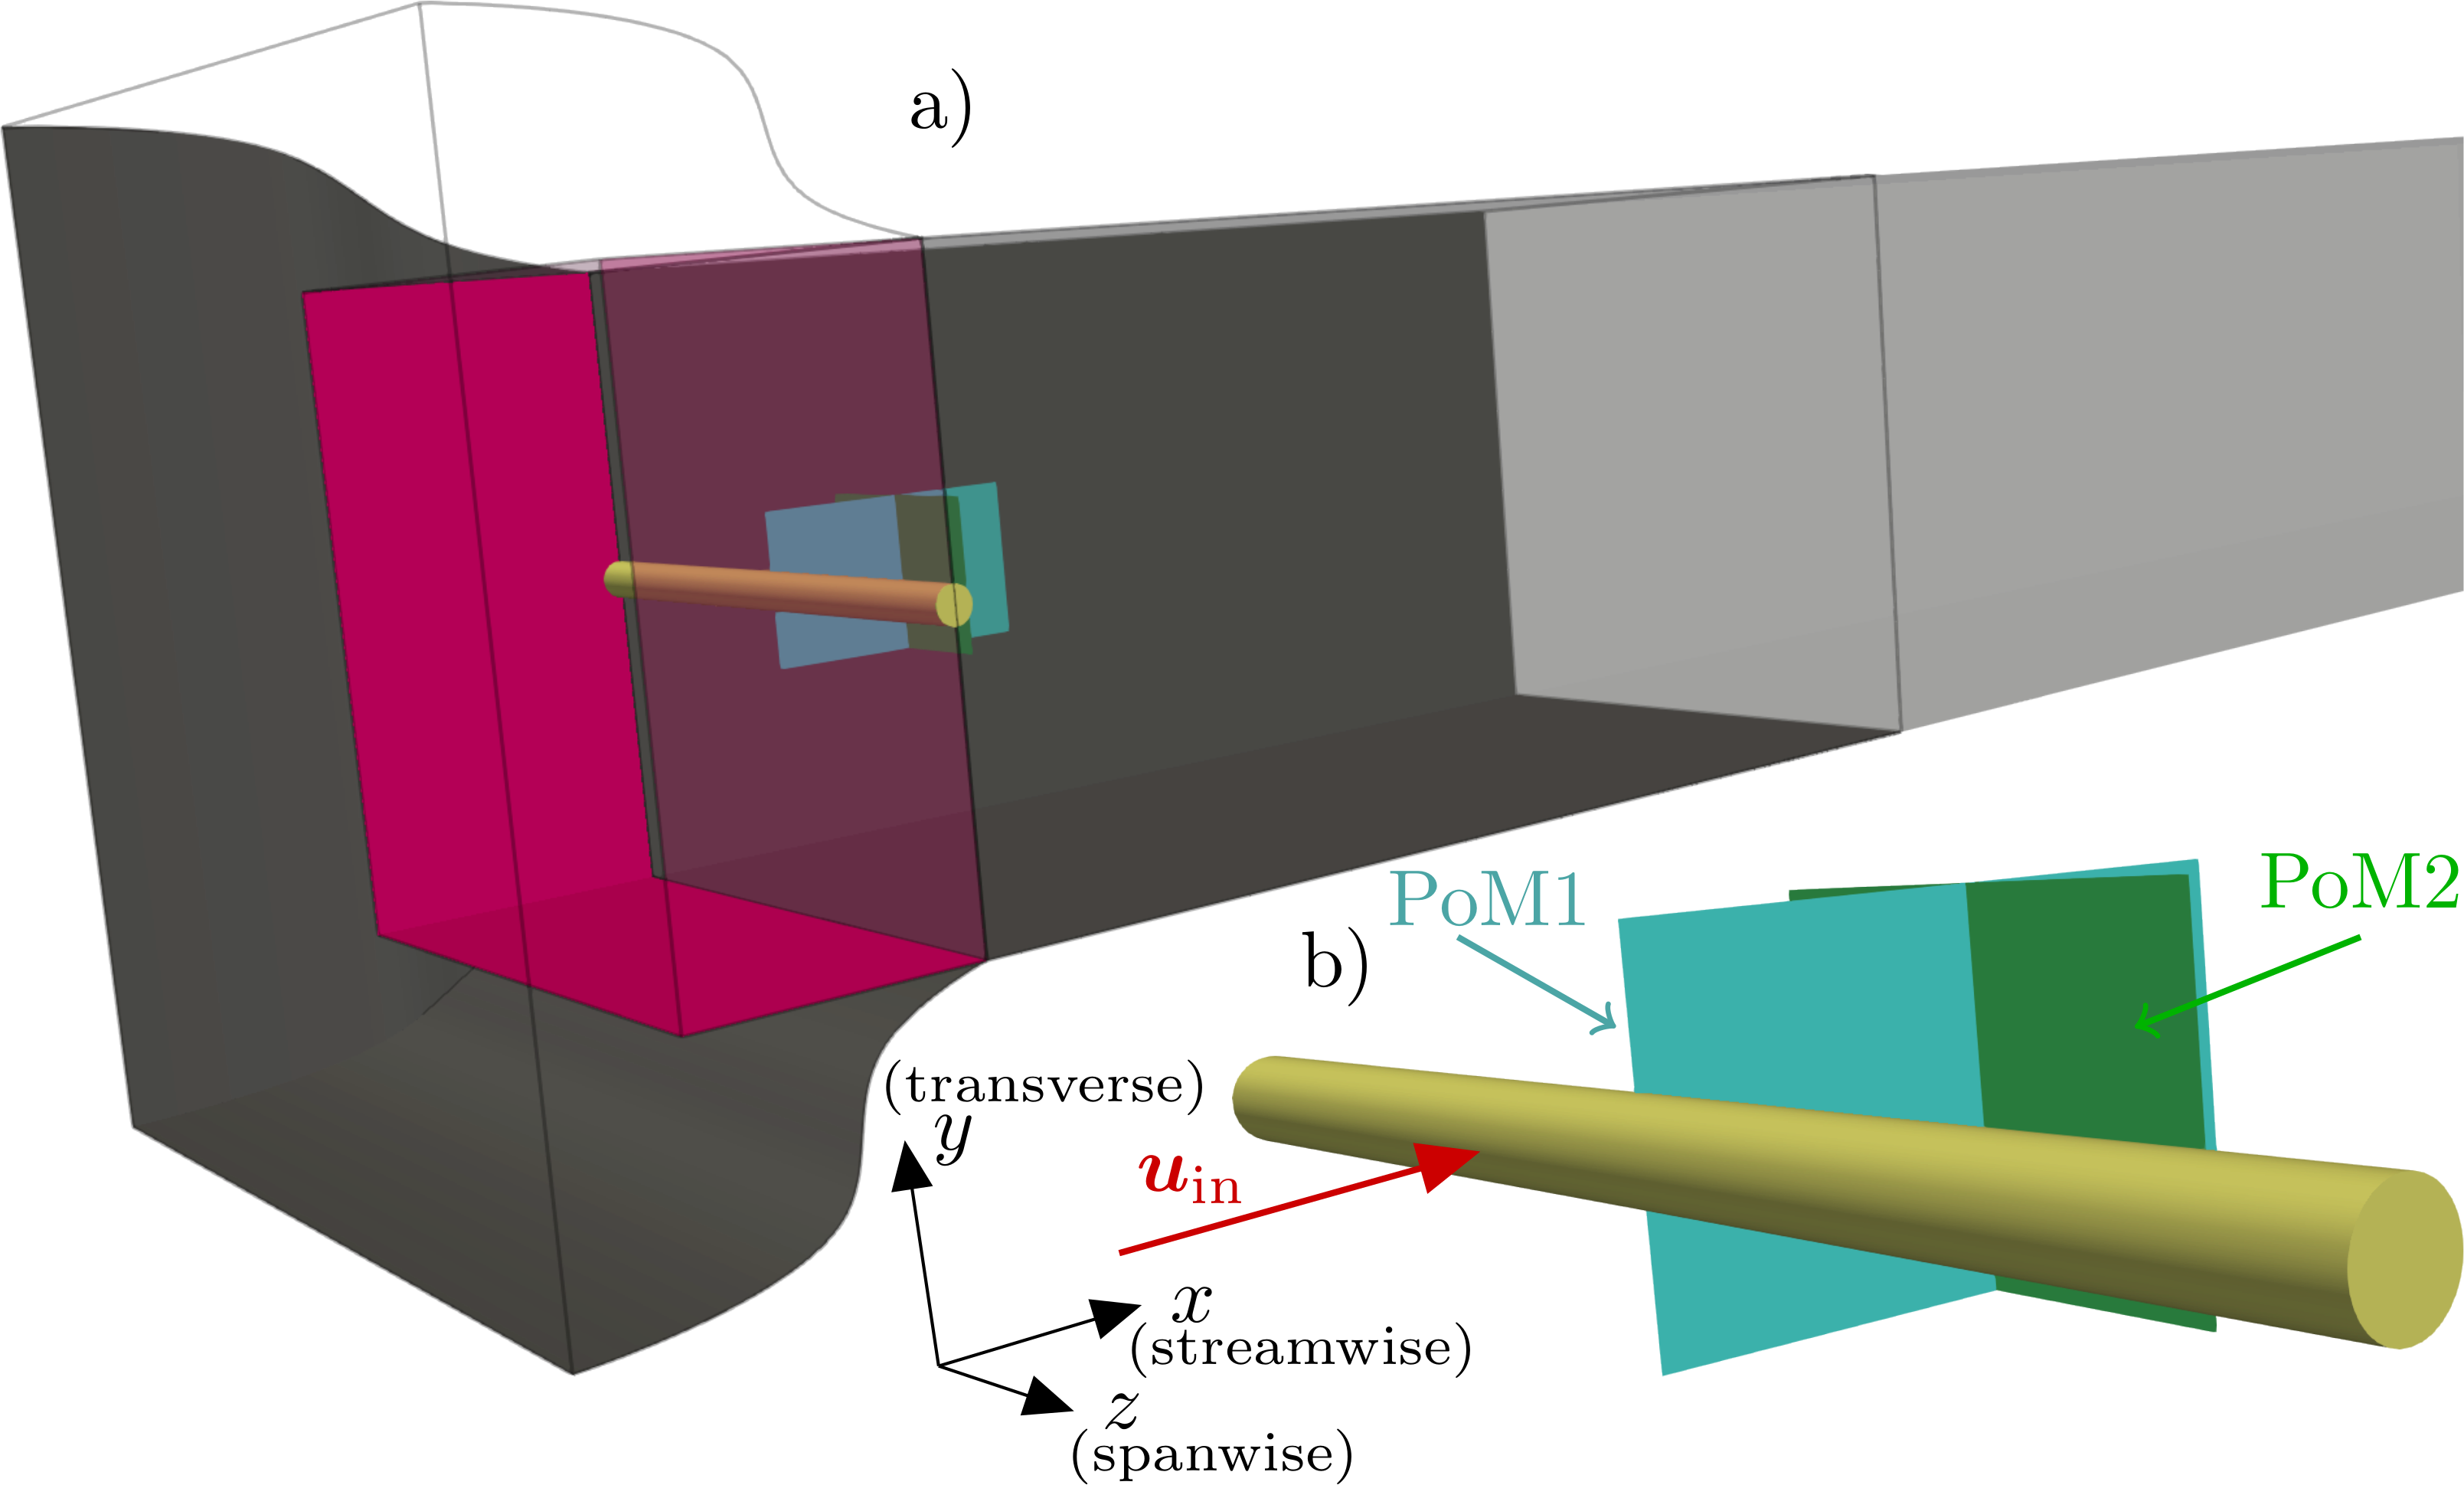
\includegraphics[width=0.98\textwidth]{02_images/00_export/figure1.png}
    \caption{(a) Sketch of the experimental set up and of the corresponding computational domain. Geometrical discrepancy between the two is highlighted in red. The planes of measurement used in experiment are shown in teal (PoM1) and green (PoM2). (b) Detail of the cylinder and planes of measurement.}
    \label{fig:geom}
\end{figure}
The problem at hand consists of the cross-flow around a circular cylinder. The experimental data were measured at a blown-down facility with a closed test section of $250\times 250\,\mathrm{mm}^{2}$. The cylinder model of diameter $d = 15 \,\mathrm{mm}$ and spanning the whole test section was placed at the test section center and oriented transversely with respect to the main flow direction as indicated in Figure~\ref{fig:geom}a. The cross-section blockage caused by the cylinder model was about $6\,\%$.{}

The experimental data on the flow field were obtained via the time-resolved Particle Image Velocimetry (PIV). The measurement apparatus comprises a laser and CMOS cameras by the Dantec company. The used laser is the New Wave Pegasus, Nd:YLF double head with wavelength of $527\, \mathrm{nm}$, maximal frequency $10\, \mathrm{kHz}$, shot energy of $10\, \mathrm{mJ}$ (for $1\, \mathrm{kHz}$) and the corresponding power of $10\, \mathrm{W}$ per one head. The cameras are the Phantom V611 and SpeedSense VEO 410 with the resolution of $1 280 \times 800$ pixels able of acquiring double snaps with frequency up to $3\, \mathrm{kHz}$ (at full resolution). The flow was visualized utilizing the SAFEX particles, i.e. oil droplets $1\,\mu \mathrm{m}$ in diameter. The data were collected and postprocessed in the DynamicStudio software \cite{dynamicsStudio}.

The flow velocity ($\bm{u} = (u,v,w)^{\transp}$) data were sampled for $2\,\mathrm{s}$ with the acquisition frequency of $2\,\mathrm{kHz}$. The data were collected on two planes of measurements (PoM) as depicted in Figure~\ref{fig:geom}b. The stream-wise oriented PoM (PoM1) lies in the $x-y$ plane. Fixing the origin of the problem cartesian coordinate system at the cylinder center of gravity {and scaling the distances by cylinder diameter $d$ as $\bm{x}_{r} = (x_r,y_{r},z_{r}) = (x,y,z)/d = \bm{x}/d$}, PoM1 is defined as 
\begin{equation}
    \label{eq:POM1}
    {\mathrm{PoM1} = \{(x_r,y_r,z_r)\in\mathbb{R}^{3}:x_r\in [0.5,7],\,y_r\in[-2,2],z_r=0\}}\,.
\end{equation}
The PoM2 lies in the $y-z$ plane in the distance of {$x_r = 3.83$} behind the cylinder, i.e. 
\begin{equation}
    \label{eq:POM1}
    {\mathrm{PoM2} = \{(x_r,y_r,z_r)\in\mathbb{R}^{3}:x_r = 3.83,\,y_r\in[-2,2],z_r\in[-3,3]\}}\,.
\end{equation}
In the PoM1, the classical variant of PIV with a single Phantom camera able to evaluate two velocity components ($u$ and $v$) was applied. In the PoM2, the stereo-PIV version with two VEO cameras was utilized and all the three velocity components ($u$, $v$ and $w$) were acquired. The velocities in PoM1 were evaluated in the mesh of {{$159\times 99$}} points in the $x$ and $y$ axis direction, respectively. The measurement mesh resolution in PoM2 was {{$61\times 91$}} points with respect to the $y$ and $z$ axis directions. A detailed description of the applied PIV system may be found in \cite{prochazka2019}.


The CFD model geometry was as close to the experimental apparatus as possible. In both the experiment and the simulation, the cylinder comes in contact with an almost uniform flow field of mean velocity $\bm{u}_{\mathrm{in}} = (u_{\mathrm{in}},0,0)^{\transp}\,\mathrm{m\,s^{-1}}$, where $u_{\mathrm{in}} = 5\,\mathrm{m\,s^{-1}}$ resulting in the aforementioned Reynolds number of $\Rey = u_{\mathrm{in}}\,d/\nu = 4815$, with $\nu$ being the fluid (air) kinematic viscosity. In the experiment, a flow field with a low turbulence of intensity $I\approx 0.2\,\%$ and a good regularity with departures below $1\,\%$ is provided by an inlet nozzle. The region inside the inlet nozzle has been modeled by a test section extension in the upstream direction to capture the cylinder effect on the upstream flow-field. The modeled test section walls in front of the cylinder were considered as impermeable but not posing any tangential resistance to the flow. As a result, the simulated flow field at the contact with the cylinder was almost uniform, similarly to the experiment. The situation is illustrated in Figure~\ref{fig:geom}a, where the special \textit{virtual walls} of the computational domain are shown in red.


\section{Mathematical model}
\label{sec:model}
A numerical CFD model of the cross flow around a circular cylinder was prepared utilizing the OpenFOAM open-source CFD library \citep{OpenFOAM2007}, which is based on the finite volume method (FVM). In the following, we first list the flow governing equations and discuss the selected approach to the turbulence modeling. Next, we concentrate on the used computational mesh and problem boundary conditions. The section is concluded by listing the applied numerical methods and by a discussion of the solution independence with respect to the selected mesh resolution.

\subsection{Flow governing equations, turbulence modeling and boundary conditions}
\label{sub:flowEqs}
Let us denote the spatial domain corresponding to the geometry shown in Figure~\ref{fig:geom} as $\Omega$ and its boundary as $\partial\Omega$. Next, let $Q = (0,T]\times \Omega$ be the complete spatio-temporal computational domain. The flow in $Q$ is assumed to be governed by the standard set of the Navier-Stokes equations for an incompressible and isothermal flow of a Newtonian fluid, i.e.
\begin{equation}
\label{eq:nsEqs}
    \begin{array}{*1{>{\displaystyle}c}}
        \frac{\partial \bm{u}}{\partial t} + \nabla \cdot \left( \bm{u} \otimes \bm{u}\right) - \nabla \cdot \bm{T} = -\nabla \tilde{p} \\[0.2cm]
        \nabla \cdot \bm{u} = 0
    \end{array}\quad \forall (t,\bm{x})\in Q
\end{equation}
where $\bm{u}$ is the fluid velocity, $\tilde{p} = p/\rho$ is the kinematic pressure obtained by dividing the pressure $p$ by the fluid density $\rho$, which is assumed to be constant in $Q$. Finally, $\bm{T}$ is the viscous stress tensor.

Due to the computational costs, not all the flow scales in $Q$ are directly simulated. Instead, the turbulent flow is solved within the large eddy simulation (LES) framework in which $\bm{u}$ and $\tilde{p}$ are replaced by their filtered counterparts $\filtU$ and $\filtP$ and the stress tensor $\bm{T}$ is decomposed as 
\begin{equation}
\label{eq:stress}
    \bm{T} = \filtT + \sgsT\,,
\end{equation}
where $\filtT$ is the filtered, or resolved scale, strain rate tensor and $\sgsT$ is the unknown subgrid scale (SGS) stress tensor that represents the effects of SGS motion on the resolved LES fields \citep{yang2015}.

Furthermore, in order to correctly and efficiently account for the spatial computational domain $\Omega$ being relatively large compared to the region of interest containing the two planes of measurement, we use a hybrid LES-RANS turbulence model introduced by \citet{strelets2001}. Within this approach, known as the detached eddy simulation (DES), a single turbulence model is used that acts as a subgrid scale model where the grid resolution is high enough and as a RANS model in the regions where it is not \citep{strelets2001}.

In the particular DES formulation used in the present work the applied turbulence model is the $k-\omega$ shear stress transport (SST) model by \citet{menter1992} as reformulated by \citet{hellsten1997} and summarized in \citep{menter2003}. The closure of the problem~\eqref{eq:stress} is based on a solution of two additional transport equations for the unknown modeled turbulence kinetic energy ($k$) and the specific dissipation rate ($\omega$). The model equations for incompressible flow are
\begin{equation}
\label{eq:kOmegaSSTDES}
    \begin{array}{*1{>{\displaystyle}c}}
        \frac{\partial {k}}{\partial t} + \nabla \cdot \left( \bm{u}\, k\right) = \tilde{P}_{k} - \beta^{*}k\,\omega\,F_{\mathrm{DES}} + \nabla \cdot \left(\left(\nu + \sigma_{k}\nu_{t}\right)\nabla k\right)\\[0.2cm]
        \frac{\partial {\omega}}{\partial t} + \nabla \cdot \left( \bm{u}\, \omega\right) = \alpha\,S^{2} - \beta\,\omega^{2} + \nabla \cdot \left(\left(\nu + \sigma_{\omega}\nu_{t}\right)\nabla \omega\right) + 2\left(1-F_{1}\right)\sigma_{w2}\frac{1}{\omega}\nabla k \cdot \nabla \omega\\[0.2cm]
        \quad \forall (t,\bm{x})\in Q
    \end{array}
\end{equation}
where the constants and parameters $\tilde{P}_{k},\,\beta^{*},\,\sigma_{k},\,\alpha,\,S,\,\beta,\,F_{1}$ and $\sigma_{w2}$ may be found for example in \citep{hellsten1997} or \citep{menter2003}. The function $F_{\mathrm{DES}}$ accounts for the DES modification to the standard $k-\omega$ SST model and is defined as
\begin{equation}
\label{eq:FDES}
    F_{\mathrm{DES}} = \max\left\{\frac{\ell_{t}}{C_{\mathrm{DES}}\Delta},1 \right\},\,\ell_{t} = \frac{\sqrt{k}}{\beta^{*}\omega},\,\Delta = \max\{\Delta_{x},\Delta_{y},\Delta_{z}\},\,C_{\mathrm{DES}} = 0.61
\end{equation}
with $\ell_{t}$ being the local turbulent length, $\Delta$ the local maximum grid spacing for a cartesian mesh and $C_{\mathrm{DES}}$ the model calibration constant. Note that the model as listed in~\eqref{eq:kOmegaSSTDES} and~\eqref{eq:FDES} may be used even on unstructured non-cartesian meshes. The only modification required lies in correctly estimating $\Delta$ on such meshes.

% Note (MI): we might have to check this and make it consistent with the OpenFOAM formulation
% https://www.openfoam.com/documentation/guides/latest/doc/guide-turbulence-des-k-omega-sst-des.html
% or it even might be already consistent... I just didn't check it

\begin{table}[htbp]
\hspace*{-2.0cm}
{
\begin{tabular}{lclclc}
\toprule
    Boundary & Conditions & Boundary & Conditions & Boundary & Conditions \\
\midrule
    \multirow{4}{*}{inlet}
    &
    $\bm{u} = (u_{\mathrm{in}},0,0)^{\mathrm{T}}$ & \multirow{4}{*}{outlet} &  $\bm{n} \cdot \bm{u} = (0,0,0)^{\mathrm{T}}$ & \multirow{4}{*}{cylinder} & $\bm{u} = (0,0,0)^{\transp}\leftarrow$ \textit{no-slip}\\
    &
    $\bm{n}\cdot\nabla p = 0$ & & $p = 0$ & & $\bm{n}\cdot\nabla p = 0$\\
    &
    $k = k_{0} \leftarrow I = 0.2\,\%$ & & $\bm{n}\cdot\nabla k = 0$ & & $k = 0$\\
    &
    $\omega = \omega_{0} \leftarrow I = 0.2\,\% $ & & $\bm{n}\cdot \nabla\omega = 0$ & & $\bm{n}\cdot \nabla\omega = 0$\\
\midrule
    \multirow{4}{*}{virtual walls}
    &
    $\bm{u}\leftarrow$ \textit{slip} & \multirow{4}{*}{walls} & $\bm{u} = (0,0,0)^{\transp}\leftarrow$ \textit{no-slip}\\
    &
    $\bm{n}\cdot\nabla p = 0$ & & $\bm{n}\cdot\nabla p = 0$\\
    &
    $\bm{n}\cdot\nabla k = 0$ & & $k \leftarrow$ wall function\\
    &
    $\bm{n}\cdot\nabla \omega = 0$ & & $\omega \leftarrow$ wall function\\
\bottomrule
\end{tabular}
}
\caption{Applied boundary conditions. The \textit{virtual walls} are shown in red in Figure~\ref{fig:geom}.}
\label{tab:BC}
\end{table}

The used boundary conditions are mostly standard and are summarized in Table~\ref{tab:BC}. However, it was necessary to resolve the geometric discrepancy between the experiment and simulation, shown in Figure~\ref{fig:geom}. The flow field at the inlet is well defined with $u_{\mathrm{in}} = 5\,\mathrm{m\,s^{-1}}$ and $I =  0.2\,\%$. Still, in the simulation, the inlet needed to be moved upstream, see the red (\textit{virtual}) walls in Figure~\ref{fig:geom}a. To keep the flow uniformity at the contact with the cylinder, the \textit{slip} boundary condition,
\begin{equation}
\label{eq:slipBC}
    \bm{u}\cdot \bm{n} = 0\quad \text{ and }\quad \bm{t}_{\mathrm{w},t} = \bm{t}_{\mathrm{w}} - \left(\bm{n}\cdot \bm{t}_{\mathrm{w}} \right)\bm{n} = 0\,,
\end{equation}
where $\bm{t}_{\mathrm{w}}$ is the wall stress vector, is applied at the \textit{virtual walls}. Finally, note that although the wall functions are used for the turbulence variables at the test section walls, the mesh resolution is such that they are effectively turned-off for most of the test-section and affect the flow solution only downstream from the region of interest.

\subsection{Computational mesh}
\label{sub:meshAndBC}
Let $\Omega^{h}$ mark the finite volume spatial discretization of $\Omega$, i.e. the computational mesh. The mesh was constructed such that the region of interest
\begin{equation}
    \label{eq:RoI}
    {\mathrm{RoI} = \{(x_r,y_r,z_r)\in\mathbb{R}^{3}:x_r\in [0,7],\,y_r\in[-2,2],z_r=\in[-3,3]\}}
\end{equation}
as well as the parts of $\Omega$ directly affecting the flow in RoI comprise a structured hex-dominant grid with the resolution sufficient to fully simulate all the relevant flow scales. On the other hand, the main purpose of the computational domain outside of RoI is to provide physically correct boundary conditions at the RoI boundaries. Thus, the mesh in these regions is coarsened and the flow there is simulated using the $k-\omega_{\mathrm{SST}}$ unsteady RANS model.

\begin{figure}[htbp]
    \hspace*{-1.5cm}
    % \begin{tikzpicture}
    %     \node (mesh) at (0,0) {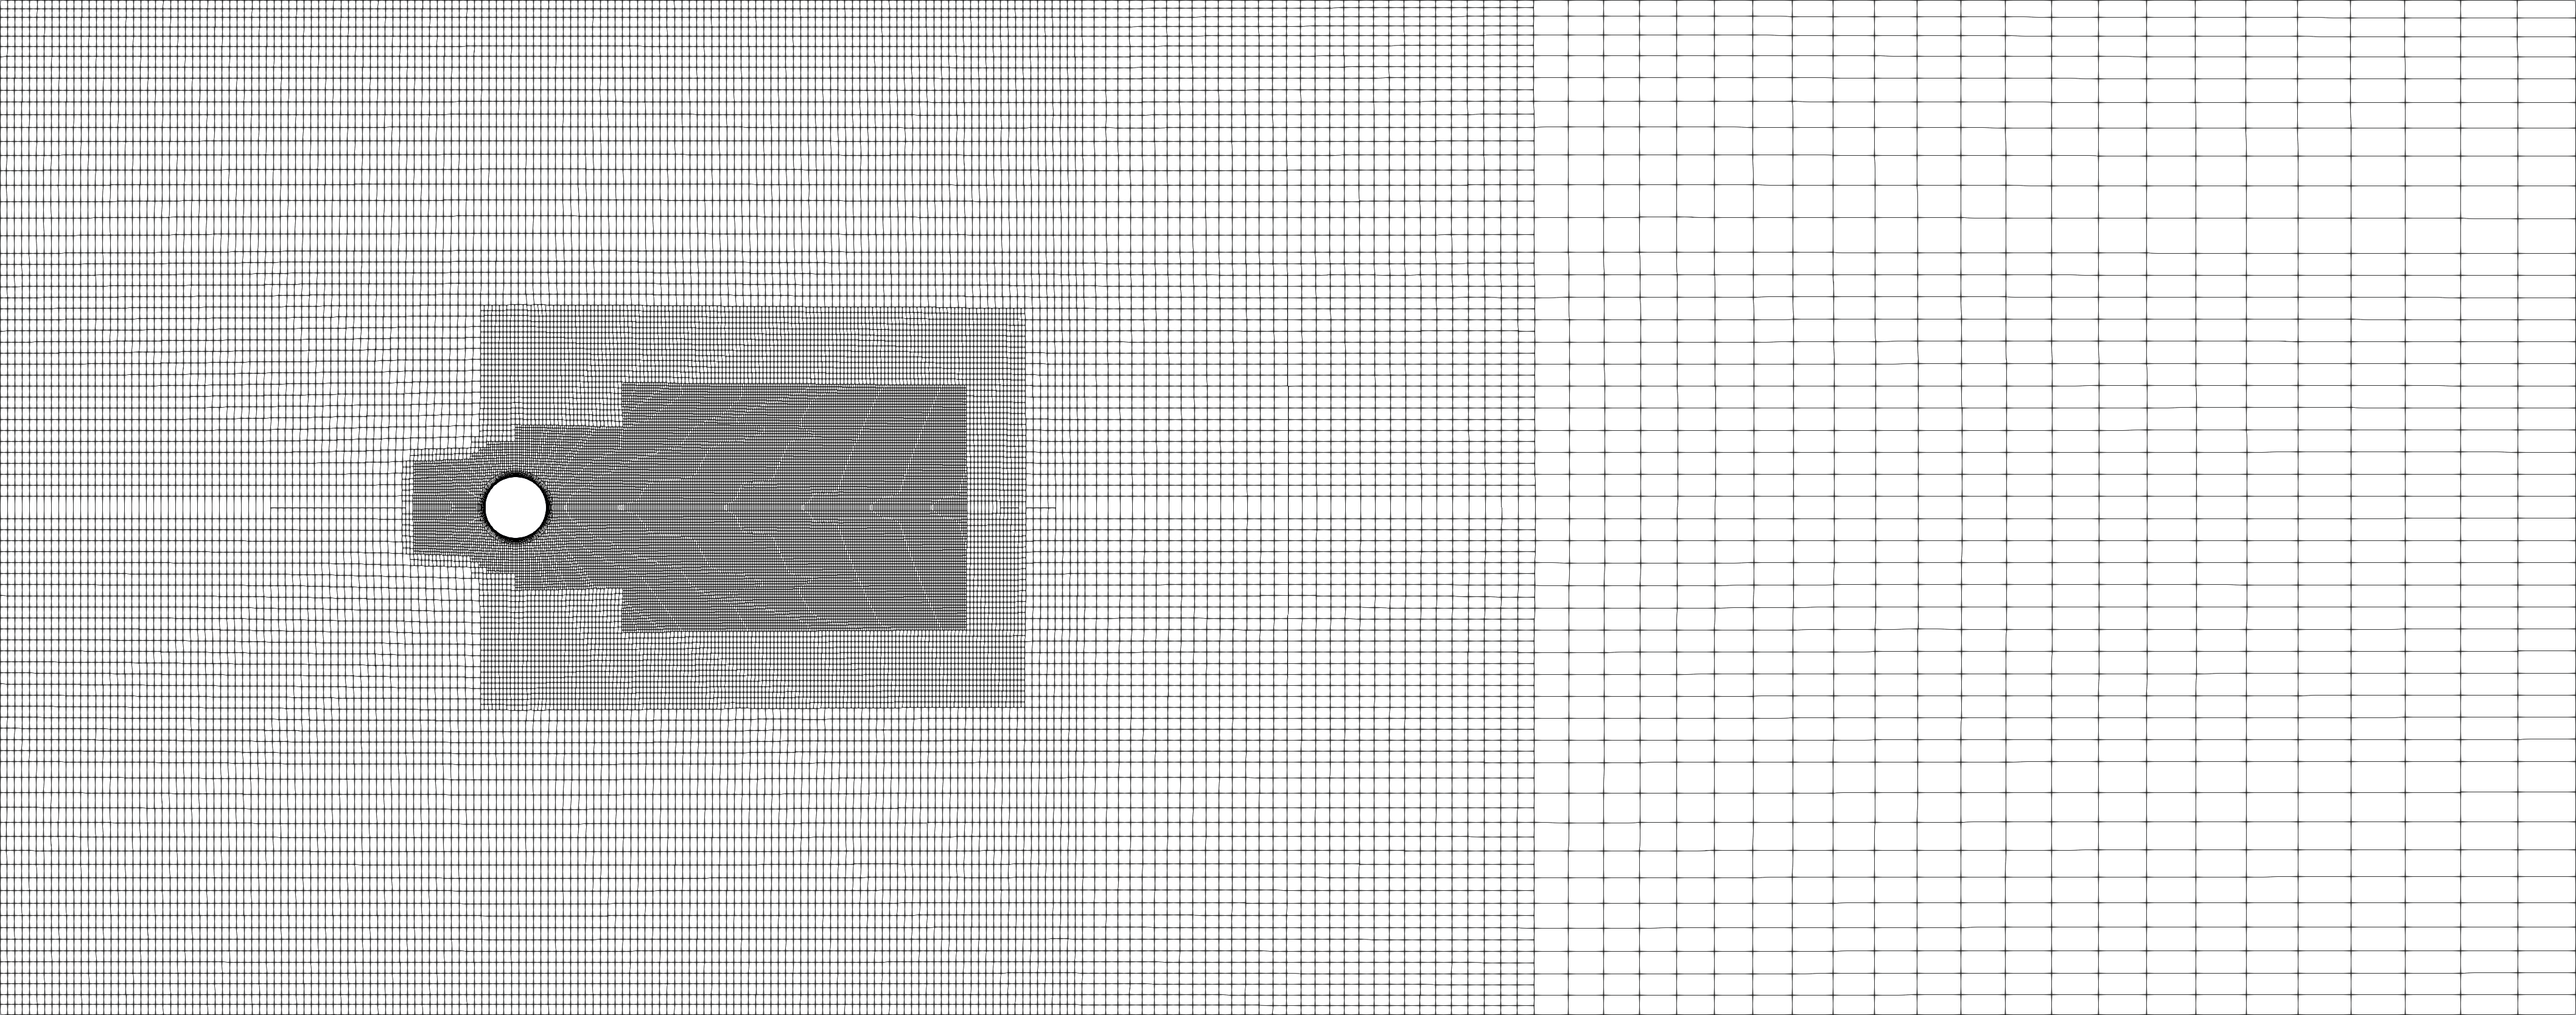
\includegraphics[width=0.9\auxWidth]{\myImages/meshSideViewV3Trp.png}};
        
    %     \draw[thick,red] (-4.63,-1.0) rectangle (-2.0,1.0);
        
    %     DNS regions
    %     \draw[thick,blue] (-5.0,-0.2) -- (-1.8,-0.9) -- (-1.8,0.9) -- (-5.0,0.2) -- cycle;
    %     \draw[thick,blue]   (-0.45\auxWidth,2.9) -- (-1.5,2.7) -- (-1.5,2.9) -- cycle;
    %     \draw[thick,blue]   (-0.45\auxWidth,-2.9) -- (-1.5,-2.7) -- (-1.5,-2.9) -- cycle;
    %     \node[blue,fill=white,draw=blue] at (-2.7,-0.34) {DNS};
        
    %     LES regions
    %     %~ \draw[thick,green!70!black] (-1.5,2.7) -- (0.45\auxWidth,2.5) -- (0.45\auxWidth,1.5) -- cycle;
    %     \draw[thick,green!70!black] (-1.5,2.7) -- (1.4,2.5) -- (1.4,-2.5) -- (-1.5,-2.7);
    %     \draw[thick,green!70!black] (-0.45\auxWidth,-2.9) -- (-0.45\auxWidth,2.9);{}
    %     \node[green!70!black,fill=white,draw=green!70!black] at (0.9,-2.25) {LES};
        
    %     RANS/URANS regions
    %     \draw[thick,brown]  (-1.5,2.9) -- (0.45\auxWidth,2.9) -- (0.45\auxWidth,-2.9) -- (-1.5,-2.9);
    %     \node[brown,fill=white,draw=brown] at (0.365\auxWidth,-2.55) {RANS/URANS};
        
    %     plane of symmetry
    %     \draw[thick,dashdotted] (-0.45\auxWidth,0) -- (0.45\auxWidth,0) node[above=-0.07cm,midway] {plane of symmetry};
        
    %     layers
    %     \node[above left=0.5cm and 0.3cm,fill=white,draw=black,anchor=east] (layers) at (mesh.east) {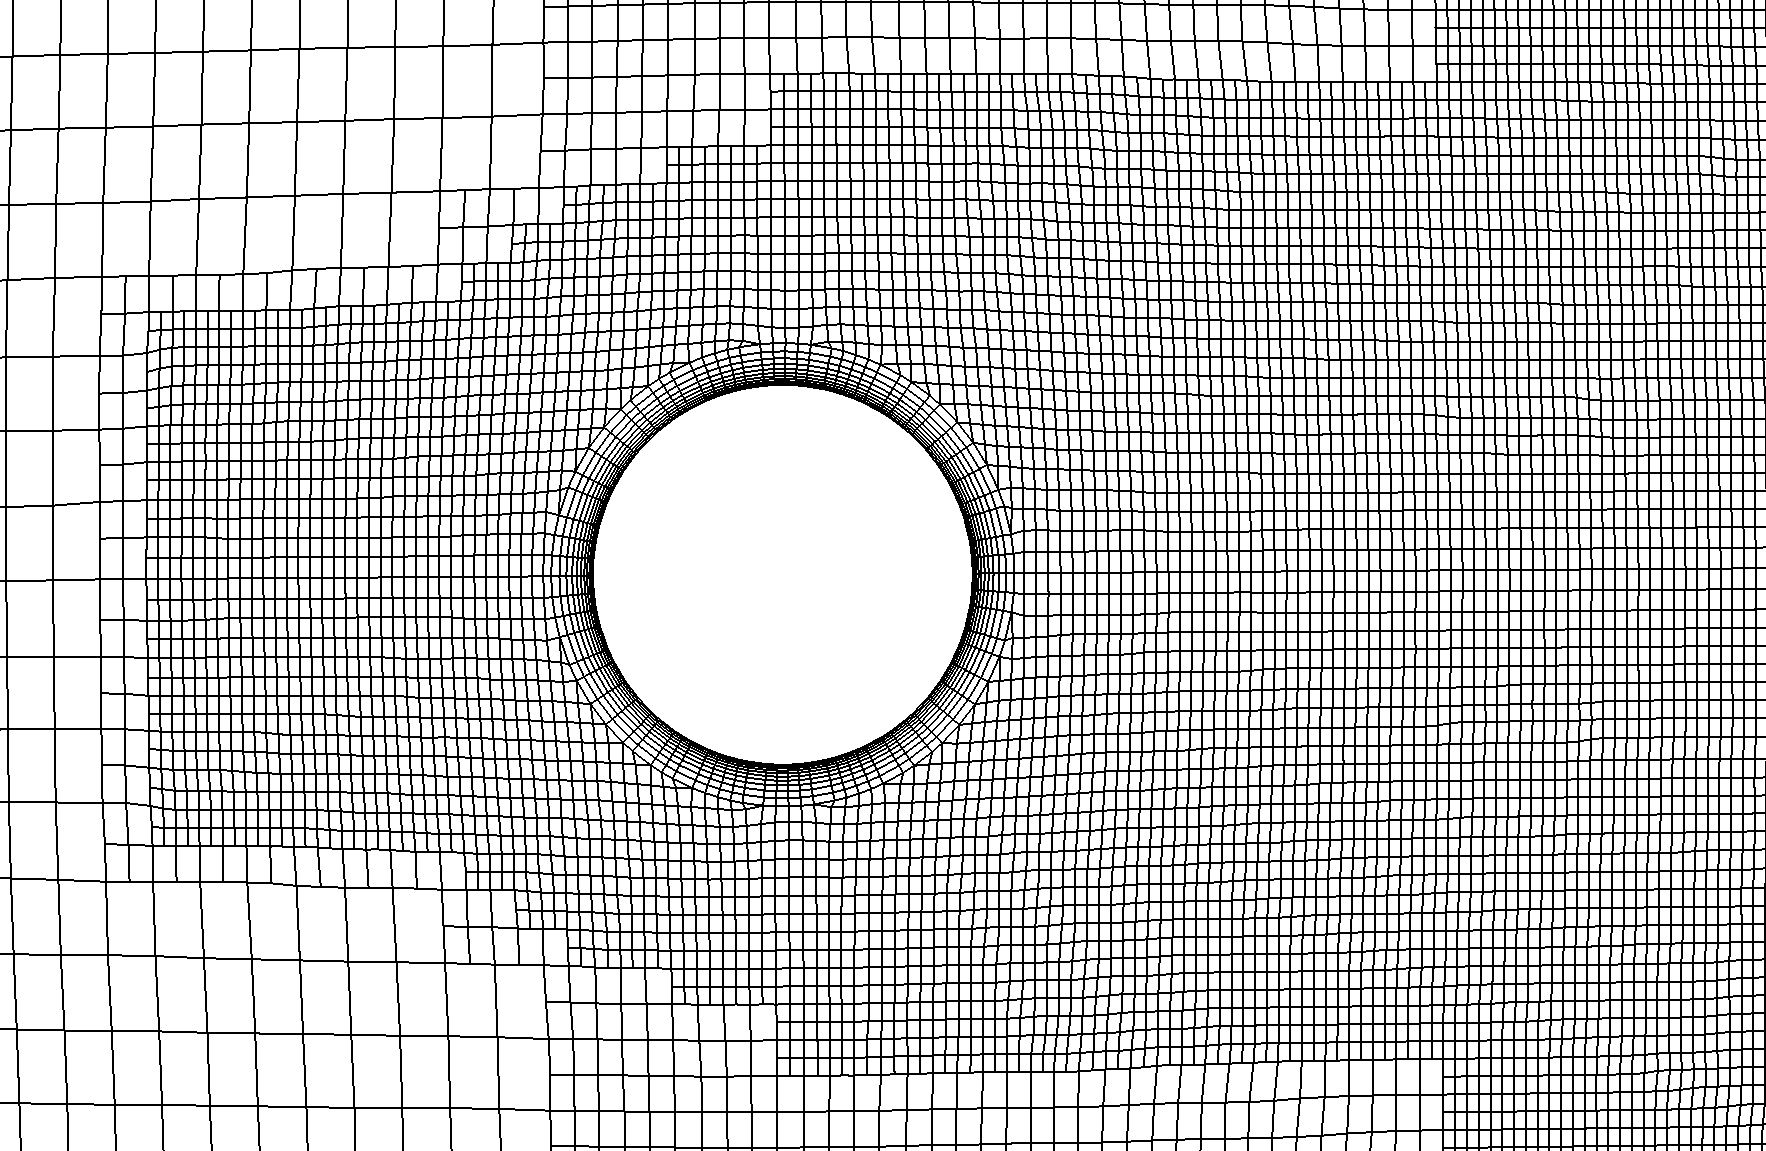
\includegraphics[width=0.31\auxWidth]{\myImages/meshSideViewDetCylV3Trp.png}};
    %     \node[anchor=south,above=0.05cm,fill=white] at (layers.south) {detail of $\Omega^{h}$ close to the cylinder};
        
    %     dimensions
    %     \draw[<->] (-0.45\auxWidth,3.3) -- (0.45\auxWidth,3.3) node[above,midway] {$L = 42.0 \,d$}; 
    %     \draw[<->] (-0.45\auxWidth,-3.3) -- (-4.63,-3.3) node[below,midway] {$L_{\mathrm{in}} = 8.5 \,d$}; 
    %     \draw[<->] (-4.63,-3.3) -- (0.45\auxWidth,-3.3) node[below,midway] {$L_{\mathrm{w}} = 33.5 \,d$}; 
    %     \draw[<->] (0.45\auxWidth,-2.9) -- (0.45\auxWidth,2.9) node[below,midway,rotate=90] {$W = 16.7 \,d = 25\,\mathrm{cm}$};
        
    % \end{tikzpicture}
    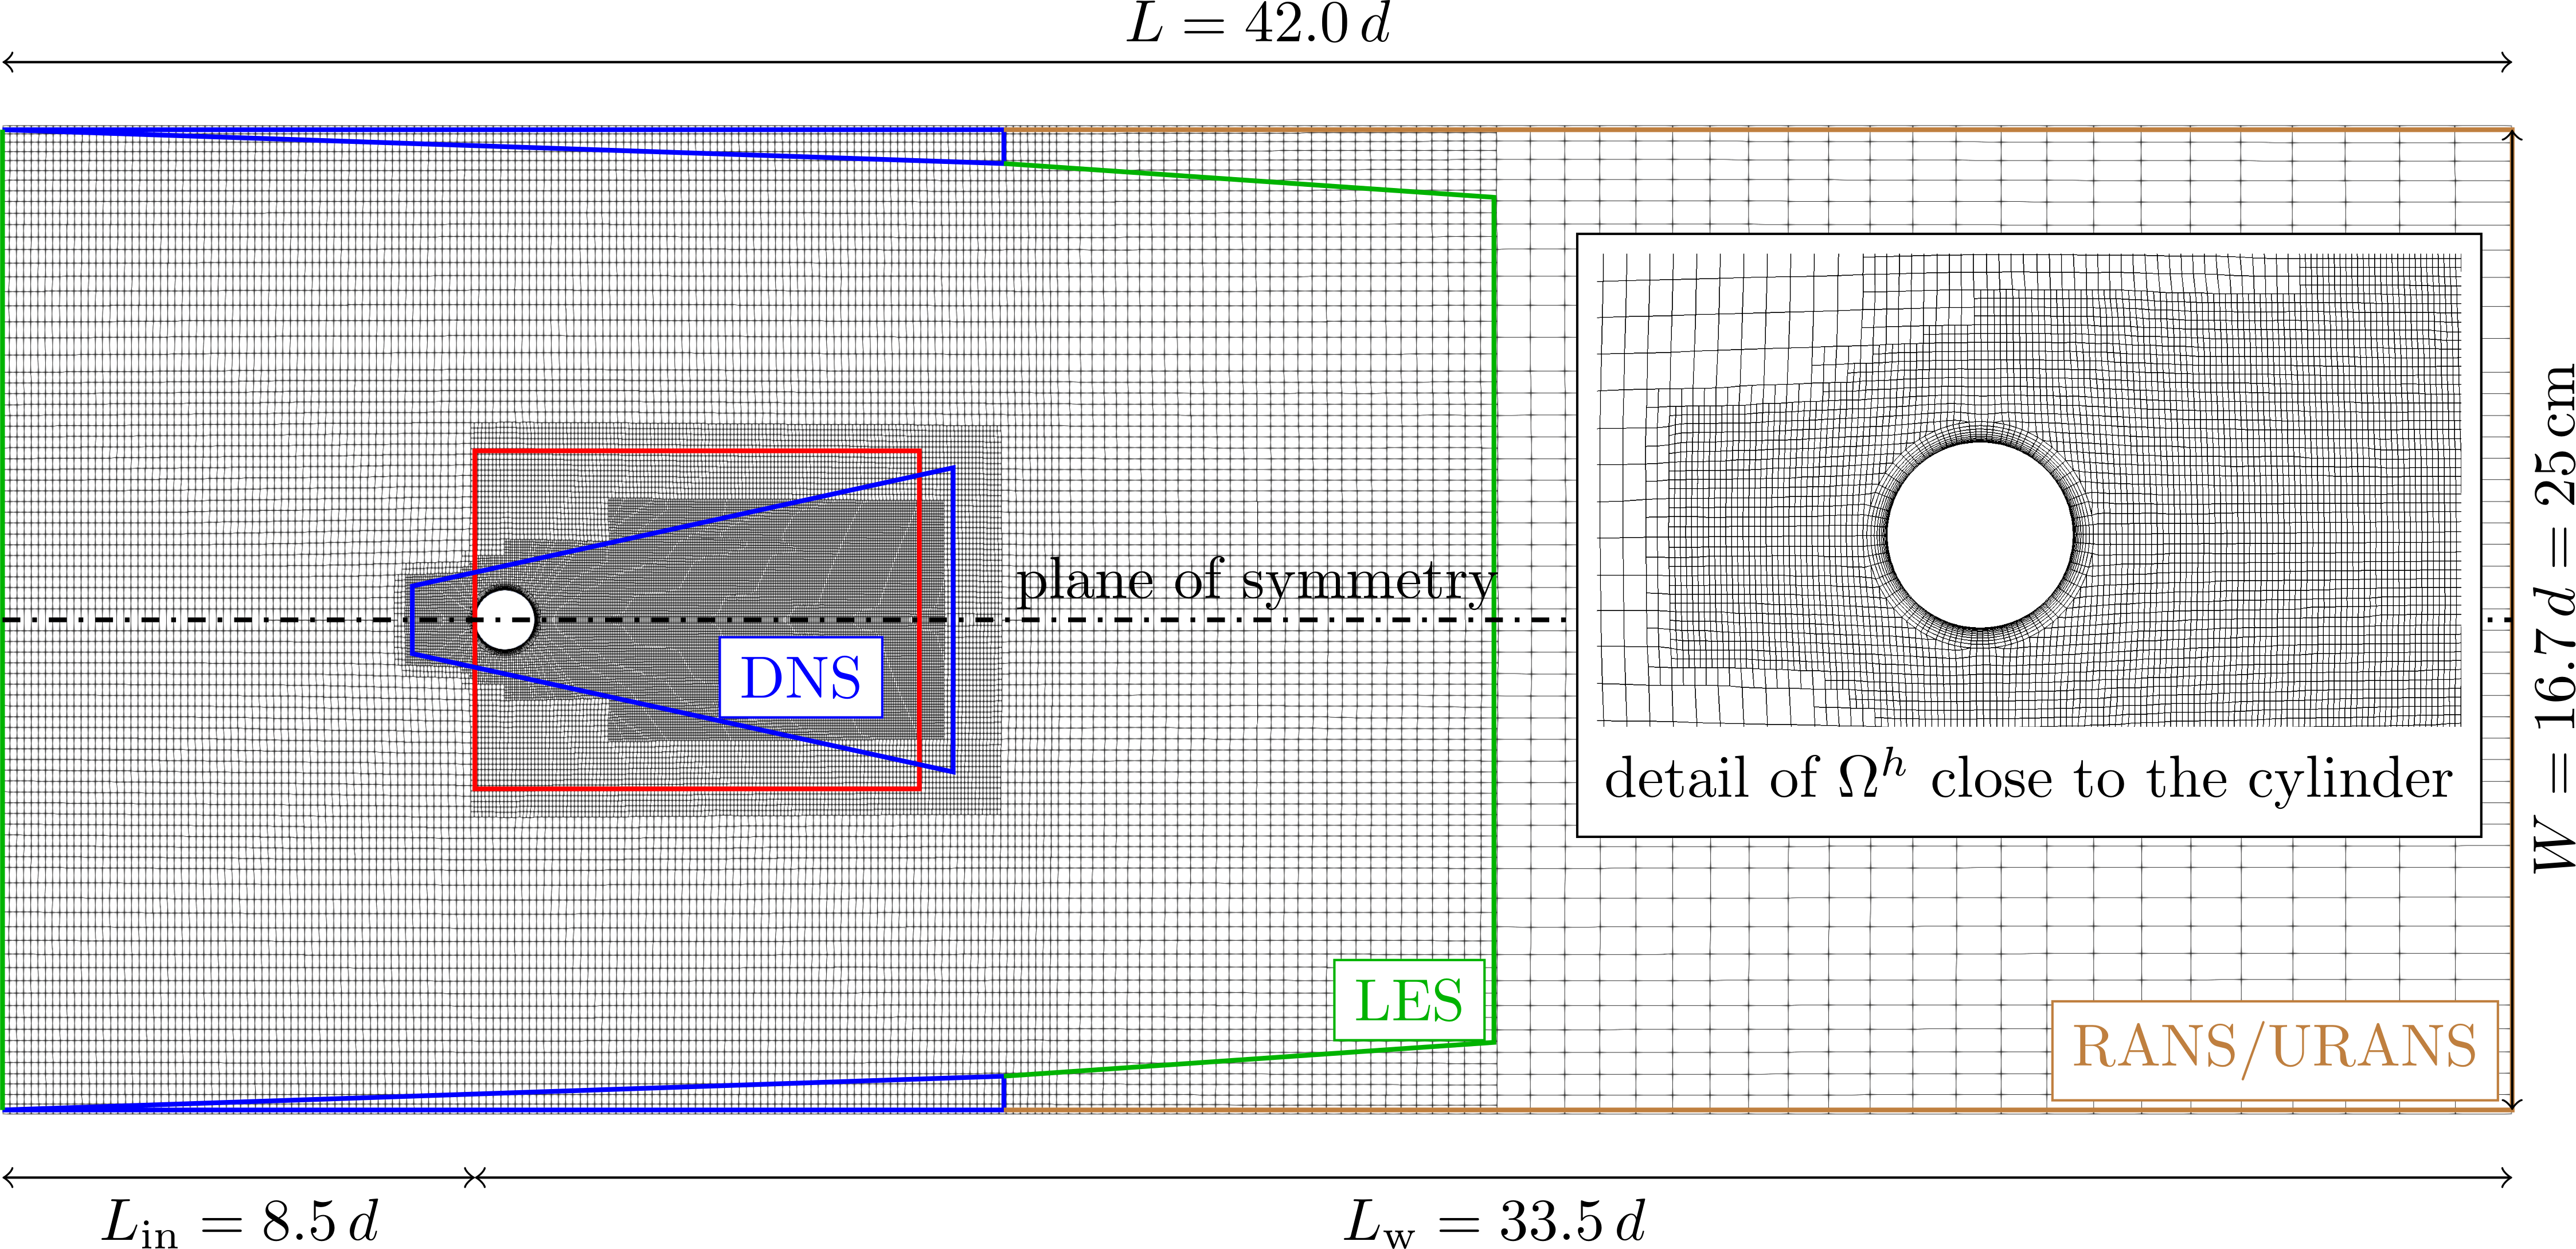
\includegraphics[width=0.98\textwidth]{02_images/00_export/figure2.png}
    \caption{Cut through the computational mesh ($\Omega^{h}$) in $x-y$ plane, which contains the streamwise plane of measurement (PoM1). Regions of activity for different turbulence models are highlighted. The region of interest (RoI) is outlined in red.}
    \label{fig:compMesh}
\end{figure}

The overall mesh structure in the $x-y$ plane is shown in Figure~\ref{fig:compMesh}. Note the high mesh resolution directly in front of the cylinder and the grid refinement towards the test section walls as indicated by the blue regions in Figure~\ref{fig:compMesh}. The high-resolution mesh in front of the bluff body is necessary to correctly resolve the pressure field, which affects the flow separation. As for the regions close to the test section walls, let us recall that at $x = 0$;
\begin{inparaenum}[(i)]
 \item in experiment, there is a transition between the inlet nozzle and the test section walls, and
 \item in simulation, there is a transition between the \textit{virtual wall} posing no tangential resistance to the flow and a standard wall.
\end{inparaenum}
Consequently, close to $x = 0$, there is a boundary layer separation on walls both in the experiment and simulation. At the studied $\Rey = 4185$, this so-called wall effect influences the wake behind the cylinder already towards the end of the region of interest and as such, it needs to be correctly resolved.

The mesh structure with respect to the $z$ axis direction is simpler than the one in the $x-y$ plane. Once more, the mesh is refined towards the test section walls. The most refined (DNS) region, which is shown in blue in Figure~\ref{fig:compMesh}, stretches between $z_{r} > -2$ and $z_{r} < 2$ and is encapsulated within the one level less refined region visible in Figure~\ref{fig:compMesh} in a way that this encapsulating region is roughly {$15\,\%$} wider than the region of interest. Finally, as shown in the detail of the mesh close to the cylinder in Figure~\ref{fig:compMesh}, ten surface layers, with the thickness increasing with the distance from the cylinder, were added onto the cylinder model in order to catch the flow separation as correctly as possible, \noteTH{resulting in an average value of yPlus $y^+_{\mathrm{avg}}\,=\,3.0\cdot10^{-6}$ and maximum at $y^+_{\mathrm{max}}\,=\,3.4\cdot10^{-5}$.}


\subsection{Numerical methods and mesh size independence}
\label{sub:numerics}
The flow governing equations were solved within {via} the finite volume method (FVM) {variant implemented in the OpenFOAM C++ library \citep{OpenFOAM2007}}. In the ideal case, FVM is second order accurate in space. However, application of the second order accurate discretization to convection terms in~\eqref{eq:nsEqs} and in~\eqref{eq:kOmegaSSTDES} leads to numerical instability even at low $\Rey$~\citep{moukalled2016}. Thus, {high-resolution} schemes switching between second and first order accuracy have been applied to the terms $\nabla \cdot \left( \bm{u} \otimes \bm{u}\right)$, $\nabla \cdot \left( \bm{u}\, k\right)$ and $\nabla \cdot \left( \bm{u}\, \omega\right)$ in~\eqref{eq:nsEqs} and~\eqref{eq:kOmegaSSTDES}, respectively. In particular, a variant of a second order upwind scheme with an explicit correction based the local gradient was used for the velocity term. For the turbulence terms, the self-filtered central differencing scheme \citep{zhu1991} was applied. The remaining spatial discretization terms were treated with the second order accuracy. Finally, the temporal integration was performed utilizing an off-centered variant of the Crank-Nicolson method \citep{crankNicolson1947}, which is close to second order accurate with respect to time.

The simulation was carried out utilizing adaptive time-stepping with the time step limited by the maximal allowed Courant number of $0.5$. The overall solution method of equations~\eqref{eq:nsEqs} and~\eqref{eq:kOmegaSSTDES} was based on the PIMPLE algorithm as implemented in OpenFOAM \citep{OpenFOAM2007}. On each time level, the system was iteratively solved until the relative residual in pressure fell under $10^{-4}$.

\begin{figure}[htbp]
    \centering
    % \begin{tikzpicture}
	\begin{axis}[
			width=0.75\linewidth,
			height = 4cm,
			scale only axis,
			name=plot1,
			xlabel=$x_r$,
			ylabel={$u_r$ [-]},
			%~ ymode=log,
			%~ xmode=log,
			ymax = 0.8,
			xmin = 0.5,
			ymin = -0.5,
			xmax = 7,
			ytick pos=left,
			mark size=4pt,    
			line width = 0.9pt,
			%~ legend style={at={(axis cs:6,2)},anchor=south west},				
		]
		% \addplot [color = black!50,mark =none]table [y=u_x,x =x]{\myGraphs/msIndData/expLineResV1.dat};\label{uxExp}
		\addplot [color = blue,mark =none]table [col sep=comma, y expr=(\thisrow{U:0})/5,x expr = {(\thisrow{Points:0})/0.015}]{\myGraphs/msIndData/mS_40p_U.csv};\label{mesh40U}
		\addplot [color = red,mark =none]table [col sep=comma, y expr=(\thisrow{U:0})/5,x expr = {(\thisrow{Points:0})/0.015}]{\myGraphs/msIndData/mS_50p_U.csv};\label{mesh50U}
		\addplot [color = green,mark =none]table [col sep=comma, y expr=(\thisrow{U:0})/5,x expr = {(\thisrow{Points:0})/0.015}]{\myGraphs/msIndData/mS_75p_U.csv};\label{mesh70U}
		\addplot [color = black,mark =none]table [col sep=comma, y expr=(\thisrow{U:0})/5,x expr = {(\thisrow{Points:0})/0.015}]{\myGraphs/msIndData/bCyl_l_3_U.csv};\label{mesh100U}
		% \addplot [color = magenta,mark =none]table [col sep=comma, y expr=(\thisrow{U:0})/5,x expr = {(\thisrow{Points:0})/0.015}]{\myGraphs/msIndData/bCyl_l_3V2_U.csv};\label{mesh110U}
		% \addplot [color = orange,mark =none]table [col sep=comma, y expr=(\thisrow{U:0})/5,x expr = {(\thisrow{Points:0})/0.015}]{\myGraphs/msIndData/mS_120p_U.csv};\label{mesh120U}
		%~ \addplot [color = red,mark =none]table [y=U_x_ms_50_U,x =z_ms_50_U]{\myGraphs/onLineMSV2.dat};\label{mesh50U}
		%~ \addplot [color = green,mark =none]table [y=U_x_ms_70_U,x =z_ms_70_U]{\myGraphs/onLineMSV2.dat};\label{mesh70U}
		%~ \addplot [color = black,mark =none]table [y=U_x_ms_100_U,x =z_ms_100_U]{\myGraphs/onLineMSV2.dat};\label{mesh100U}
		%~ \addplot [color = black,mark =none]table [y=U_x_ms_100_U,x =z_ms_120_U]{\myGraphs/onLineMSV2.dat};\label{mesh100U}
		\coordinate (top) at (rel axis cs:0,1);
		\end{axis}
    \begin{axis}[
			width=0.75\linewidth,
			height = 4cm,
			scale only axis,
			xlabel=$x_r$,
			%~ ylabel={\textcolor{red}{TKE}},
			ylabel={$k$ [-]},
			%~height=\figHeight,
			scale only axis,
			%~ xmin=0,
			%~ xmax=600,
			xmin=0.5,
			xmax=7,
			ymin=0,
			ymax = 0.3,
			%~ ymax=1000,
			hide x axis,
			line width = 0.9pt,
			axis y line*=right,
			%~ axis line style={red},
			%~ axis y label/.append style ={red},
			%~ ytick label/.append style = {red},
			%~ ylabel={$y_{\mathrm{NO}},\,y_{\mathrm{N_{2}O}} \mathrm{\,[ppm]}$},
			mark size=2.5pt, 
        ]
		% \addplot [color = black!50,mark =none,dashed]table [y=k,x =x]{\myGraphs/msIndData/expLineResKV1.dat};\label{kExp}
        \addplot [color = blue,mark =none,dashed]table [col sep=comma, y expr=(\thisrow{k}),x expr = {(\thisrow{Points:0})/0.015}]{\myGraphs/msIndData/mS_40p_k.csv};\label{mesh40k}
        \addplot [color = red,mark =none,dashed]table [col sep=comma, y expr=(\thisrow{k}),x expr = {(\thisrow{Points:0})/0.015}]{\myGraphs/msIndData/mS_50p_k.csv};\label{mesh50k}
        \addplot [color = green,mark =none,dashed]table [col sep=comma, y expr=(\thisrow{k}),x expr = {(\thisrow{Points:0})/0.015}]{\myGraphs/msIndData/mS_75p_k.csv};\label{mesh70k}
        \addplot [color = black,mark =none,dashed]table [col sep=comma, y expr=(\thisrow{k}),x expr = {(\thisrow{Points:0})/0.015}]{\myGraphs/msIndData/bCyl_l_3_k.csv};\label{mesh100k}
		% \addplot [color = magenta,mark =none,dashed]table [col sep=comma, y expr=(\thisrow{k}),x expr = {(\thisrow{Points:0})/0.015}]{\myGraphs/msIndData/bCyl_l_3V2_k.csv};\label{mesh110k}
        % \addplot [color = orange,mark =none,dashed]table [col sep=comma, y expr=(\thisrow{k}),x expr = {(\thisrow{Points:0})/0.015}]{\myGraphs/msIndData/mS_120p_k.csv};\label{mesh120k}

		\coordinate (bot) at (rel axis cs:1,0);
\end{axis}

    \matrix[
        matrix of nodes,
        anchor=south,
        draw,
        inner sep=0.2em,
        %~ thick,
        fill=white,
      ]at([xshift=0,yshift=0.2cm]plot1.south)
      {
        %~ \ref{100}& CFD old &[5pt]\\
        %~ \ref{60}& XPF - reac, wall&[5pt]\\
		% \ref{uxExp}& exp U &
        % \ref{mesh100U}& $u$ &
        \ref{mesh40U}& 3.5M cells &
        % \ref{uxExp}& $U$ exp &[5pt]\\
        \ref{mesh50U}& 5.0M cells & \\
        \ref{mesh70U}& 7.4M cells &
        \ref{mesh100U}& 8.3M cells & 
		% \ref{mesh110U}& 110 U &
        % \ref{mesh120U}& 120 U\\
		% \ref{kExp}& exp k &
        % \ref{mesh100k}& $k$ &
        % \ref{mesh40k}& 40 k &
        % % \ref{uxExp}& $U$ exp &[5pt]\\
        % \ref{mesh50k}& 50 k &
        % \ref{mesh70k}& 75 k &
        % \ref{mesh100k}& 100 k &
		% \ref{mesh110k}& 110 k &
        % \ref{mesh120k}& 120 k
		\\
%        \ref{legendNoReact}& $\mathrm{thermic\ no\ reaction\ heat}$&[5pt]
        \\};
	\matrix[
        matrix of nodes,
        anchor=east,
        draw,
        inner sep=0.2em,
        %~ thick,
        fill=white,
      ]at([xshift=-0.2cm,yshift=0cm]plot1.east)
      {
        %~ \ref{100}& CFD old &[5pt]\\
        %~ \ref{60}& XPF - reac, wall&[5pt]\\
		% \ref{uxExp}& exp U
		
        \ref{mesh100U}& $u_r$ \\
		% \ref{mesh110U}& 110 U &
        % \ref{mesh120U}& 120 U\\
		% \ref{kExp}& exp k &
        \ref{mesh100k}& $k$ &
        % \ref{mesh40k}& 40 k &
        % % \ref{uxExp}& $U$ exp &[5pt]\\
        % \ref{mesh50k}& 50 k &
        % \ref{mesh70k}& 75 k &
        % \ref{mesh100k}& 100 k &
		% \ref{mesh110k}& 110 k &
        % \ref{mesh120k}& 120 k
		\\
%        \ref{legendNoReact}& $\mathrm{thermic\ no\ reaction\ heat}$&[5pt]
        \\};
	\end{tikzpicture}

    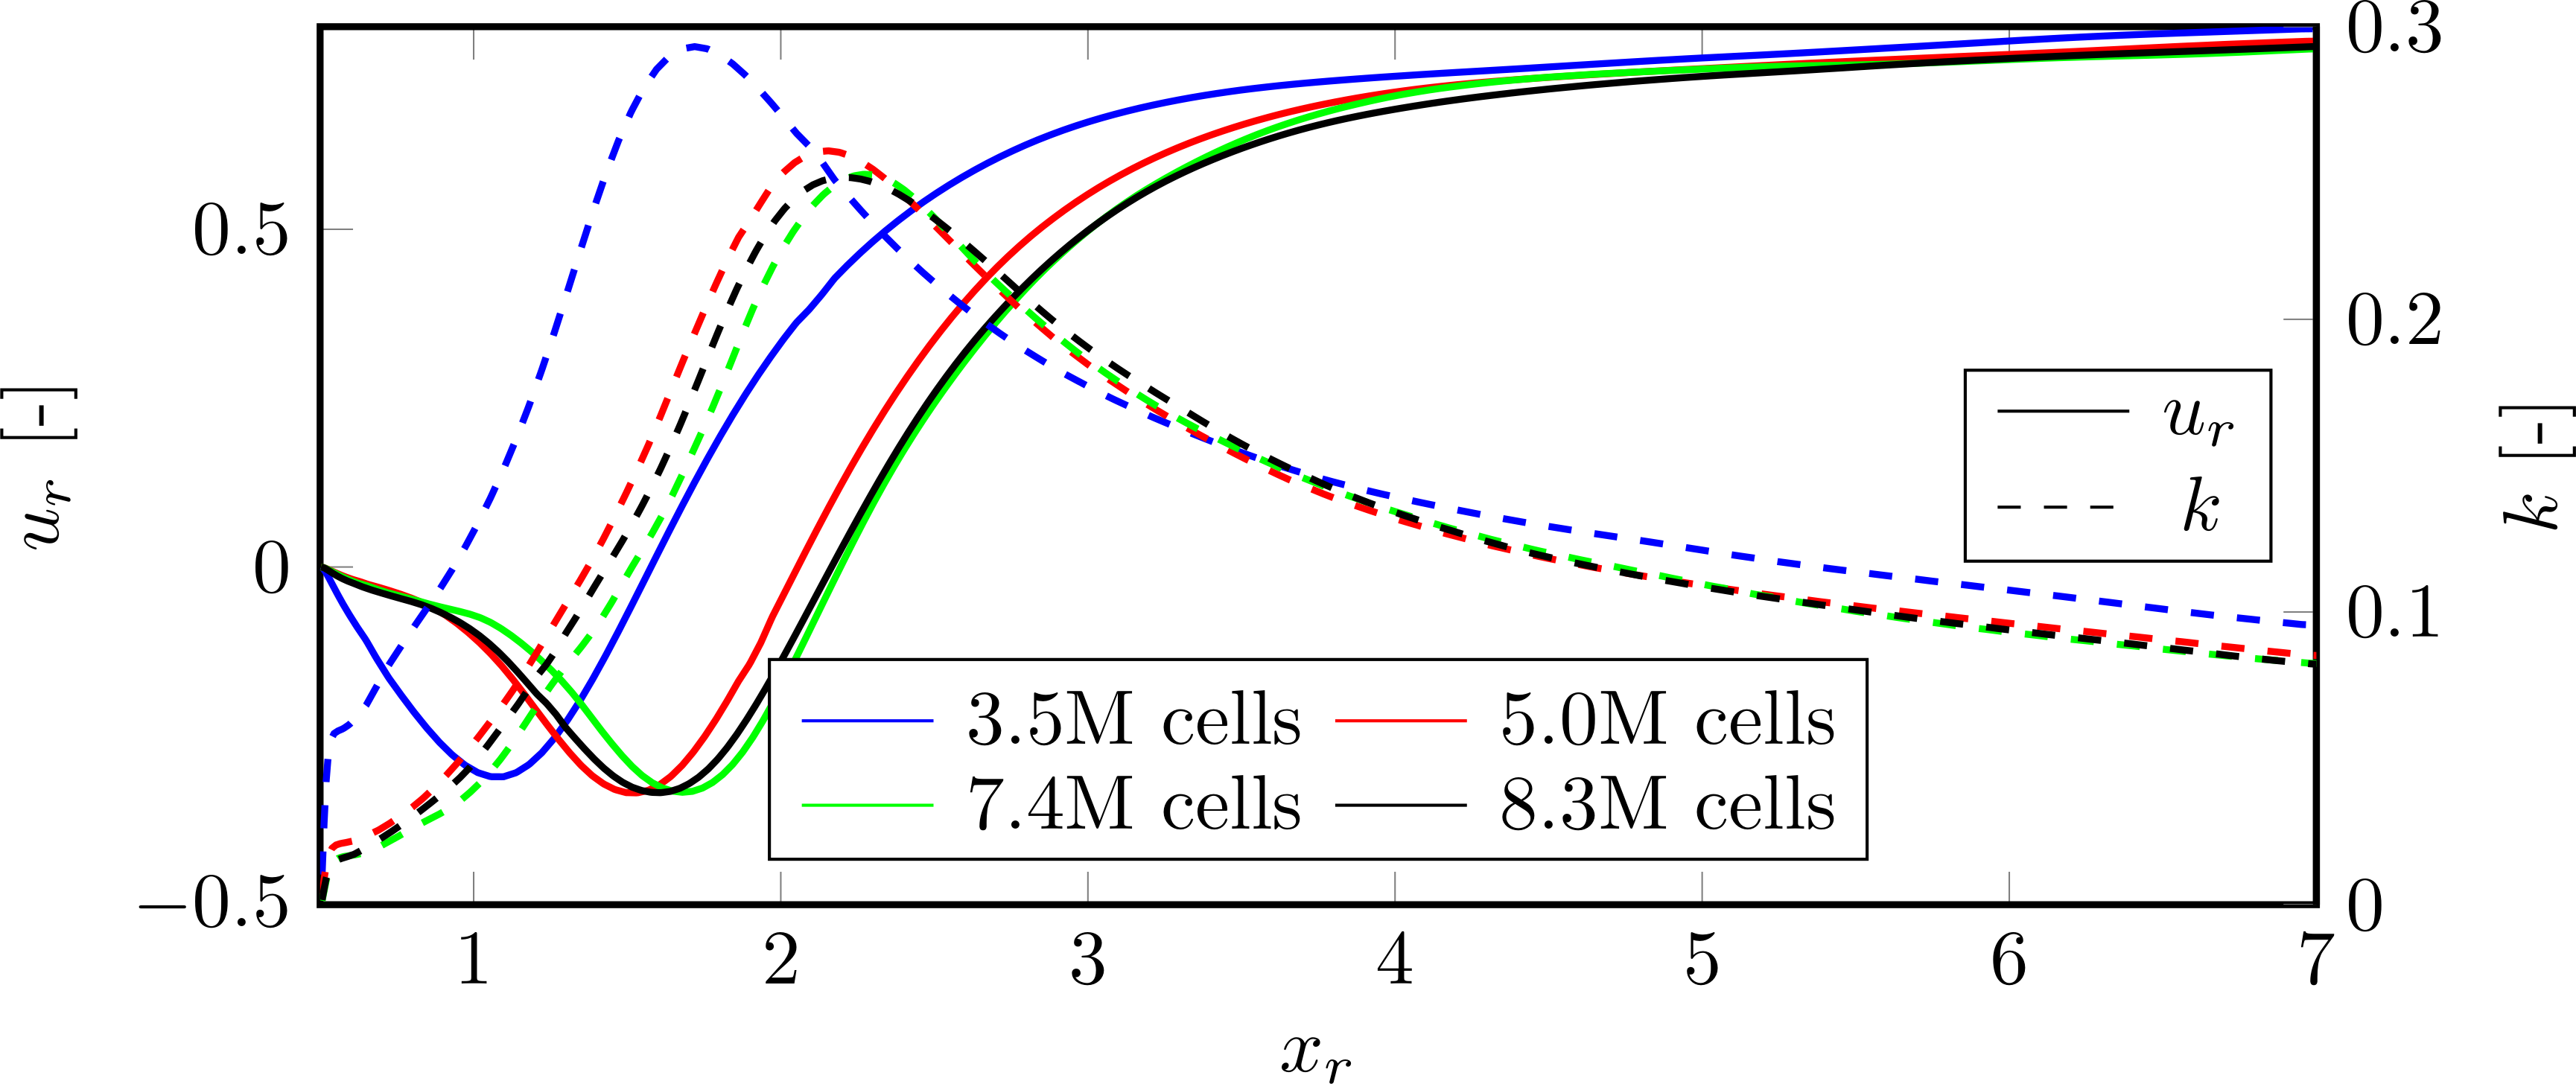
\includegraphics[width=0.98\textwidth]{02_images/00_export/figure3.png}
    \caption{Comparison of the scaled mean flow stream-wise velocity $u_r$ and turbulence kinetic energy $k$ profiles on line $\sigma$ in PoM1 for computational meshes comprising 3.5, 5.0, 7.4 and 8.3 million FV cells.}
    \label{fig:meshIndep}
\end{figure}
In order to obtain mesh resolution independent results, the simulation of flow around a cylinder was repeated four times on four different meshes with varying cell size. In Figure~\ref{fig:meshIndep}, a comparison of the {scaled} mean stream-wise velocity component, $u_r = u/u_{\mathrm{in}}$, and turbulence kinetic energy $k$ profiles on line
\begin{equation}
    {\sigma = \{(x_r,y_r,z_r)\in\mathbb{R}^{3}:x_r\in [0.5,7],\,y_r = 0,z_r=0\}}
\end{equation}
are given for meshes comprising $3.5$, $5.0$, $7.4$ and $8.3$ million{s of} finite volume cells. Increasing number of cells in computational mesh and consequent shrinking of the cell size gradually leads to more similar results. {The mesh with 7.4 million of cells was selected as the one providing a suitable trade-off between the simulation accuracy and overal computational costs. Thus, } all the results presented in \nameref{sec:resultsAndDisc} section are computed on {this mesh}.





\section{Proper orthogonal decomposition}
\label{sec:POD}

{The proper orthogonal decomposition (POD) is a robust method identifying high-energy coherent structures in spatio-temporal data. Consequently, POD is often applied in the fields of turbulence analysis \citep{uruba2020,taira2020} and modeling \citep{gatski1991,shinde2020}. As a purely data-driven technique, it can be readily used to analyze both experimental and numerical data.}

%~ One of the possible applications of the proper orthogonal decomposition (POD) lies in identification of high-energy coherent structures in spatio-temporal data. Consequently, POD is often applied in the fields of turbulence analysis \citep{uruba2020,taira2020} and modeling \citep{gatski1991,shinde2020}. Simultaneously, POD is a purely data-driven and robust method and as such, it can be readily used to analyze both experimental and numerical data.


% {====ONLY COPY-PASTE=====}

Both the experimental and simulation data are generated by sampling the studied system at given times,
\begin{equation}
\label{eq:snapshots}
    \bm{S} = \left\{\bm{y}_{j}:=\bm{y}(t_{j}) \right\}_{j=1}^{n}\,,\quad t_{j}\in (0,T]\,,
\end{equation}
where $\bm{S}$ is a set of system \textit{snapshots} and $\bm{y}_{j}$ is the vector of data at time $t_{j}$.

If all the system snapshots have the same dimension, i.e. $\bm{y}_{j}\in\mathbb{R}^{m}\,,j=1,\dots,n$, the set $\bm{S}$ may be rearranged into the matrix of snapshots
\begin{equation}
\label{eq:matrixOfSnapshots}
    Y = \left[\bm{y}_{1},\dots,\bm{y}_{n}\right] \in \mathbb{R}^{m\times n}\,,\quad \mathrm{rank}\,(Y) = n\,\,
\end{equation}
where we assumed that the number of system snapshots $n$ is lower than the data dimension $m$, which is commonly true for both the experimental and numerical data.

The standard POD algorithms are based on the singular value decomposition (SVD) of the matrix $Y$. 
\begin{equation}
\label{eq:svdY}
\begin{array}{*1{>{\displaystyle}c}}
    Y = \Psi \Sigma \Phi^{\transp}\,,\Psi \in \mathbb{R}^{m\times m}, \Phi\in\mathbb{R}^{n\times n}, \Sigma = \mathrm{diag}\,(\sigma_{1},\dots,\sigma_{m}) \in \mathbb{R}^{m\times n}\\[0.3cm]
    \Psi\Psi^{\transp} = E_{m}\,,\,\Phi\Phi^{T} = E_{n}\,,\,\sigma_{1}\geq\sigma_{2}\geq\dots\geq\sigma_{n} > 0 = \sigma_{n+1} = \dots = \sigma_{m}
\end{array}    
\end{equation}
where $E_{m}$ and $E_{n}$ are identity matrices in $\mathbb{R}^{m\times m}$ and $\mathbb{R}^{n\times n}$, respectively, and the first $n$ columns of the matrix $\Psi$ form an orthonormal basis of the column space of the matrix $Y$, i.e.
\begin{equation}
\label{eq:chronosTopos}
    \bm{y}_{j} = \Psi_{n}\bm{\eta}_{j}\,,\quad H = \left[\bm{\eta}_{1},\dots,\bm{\eta}_{n}\right]:= \Psi_{n}^{\transp} Y\,,\,\Psi_{n} = \left[\bm{\psi}_{1},\dots,\bm{\psi}_{n} \right]\in\mathbb{R}^{m\times n}\,.
\end{equation}
In~\eqref{eq:chronosTopos}, each column $\bm{\psi}_{j},\,j=1,\dots,n$ of the matrix $\Psi_{n}$ represents a temporally coherent spatial structure, \textit{topos}. Furthermore, at any time $t_{j}$, the corresponding data vector $\bm{y}_{j}$ may be reconstructed as a linear combination of toposes, utilizing the coefficients $\bm{\eta}_{j}$. Thus, each row $j$ of the matrix $H\in\mathbb{R}^{n\times n}$ represents the temporal evolution of the contribution of the topos $\bm{\psi}_{j}$ to the reconstruction of the vector $\bm{y}_{j}$, \textit{chronos}.

Finally, let us note that given the SVD properties, the toposes are sorted in descending order by the amount of variance in the original data they represent. In particular, if the data $\bm{y}_{j},\,j=1,\dots,n$ correspond to the flow velocity field fluctuations $\bm{u}' = \bm{u} - \mathrm{mean}(\bm{u})$, the POD modes are ordered by the amount of the total turbulent kinetic energy they hold. The importance of each topos $\bm{\psi}_{j}$ is proportional to the corresponding singular value $\sigma_{j}$.

\paragraph{Computational remark:} The standard approach to POD analysis is to first compute the full matrix $\Psi_{n}$ and to subsequently truncate {it} as $\Psi_{\ell} = [\bm{\psi}_{1},\dots,\bm{\psi}_{\ell}]\in\mathbb{R}^{m\times \ell},\,{\ell < n,}$ based on a cut-off energy level, i.e. the error in the Frobenius norm in the $Y$ matrix reconstruction \citep{isoz2019,volkwein2013}.  However, such a task usually requires the matrix $Y$ to be loaded into the computer memory, which may prove {to be} a problem when processing a fully three-dimensional LES simulation data \citep{kabir2017}.

\begin{algorithm}[H]
    \centering
    \caption{Out-of-memory randomized POD modes computation}
    \label{alg:randPOD}
    \begin{algorithmic}[1]
    	\Require{matrix of snapshots $Y$, POD rank $\ell$, number of power iterations $r$}
        \State Generate Gaussian random $P\in\mathbb{R}^{n\times \ell}$
        \State Compute $\tilde{Y} := YP \in\mathbb{R}^{m\times \ell}$\label{alg:tildeYComp}
        \For{$k = 1 \, \mathbf{to} \, r$}
        \State update $\tilde{Y}:= Y (Y^{\transp}\tilde{Y})$\label{alg:tildeYUpdate}
        \EndFor
        \State Decompose $\tilde{Y} = QR\rightarrow Q\in\mathbb{R}^{m\times \ell}$
        \State Compute $B = Q^{\transp}Y\in\mathbb{R}^{\ell\times n}$\label{alg:BComp}
        \State Compute $\tilde{\Psi}_{\ell},\Sigma_{\ell},\Phi_{\ell} = \mathrm{svd}\,(B)$
        \Statex\Return $\Psi_{\ell} = Q\tilde{\Psi}_{\ell},\Sigma_{\ell},\Phi_{\ell}$
    \end{algorithmic}
\end{algorithm}
In order to limit the memory demands of POD modes computation, we employed an out-of-memory randomized SVD algorithm stemming from the works \citep{rokhlin2009,halko2011,gu2015}. Utilizing this approach, the number of modes of interest $\ell \ll n = \mathrm{rank}\,(Y)$ needs to be known a-priori. The POD modes computation is based on a generation of a Gaussian random matrix $P\in\mathbb{R}^{n\times \ell}$ and summarized in Algorithm~\ref{alg:randPOD}. Note that all the computations involving the original matrix $Y$, i.e. the lines~\ref{alg:tildeYComp}, \ref{alg:tildeYUpdate} and~\ref{alg:BComp} of Algorithm~\ref{alg:randPOD} may be decomposed into a series of outer vector products and the matrix $Y$ does not have to be fully loaded into the computer memory.

% {====ONLY COPY-PASTE(END)=====}

\begin{figure}[htbp]
    \centering
    % \includegraphics[width=1.0\textwidth]{example-image-golden}
    % \begin{tikzpicture}
	\savebox\mygraphic{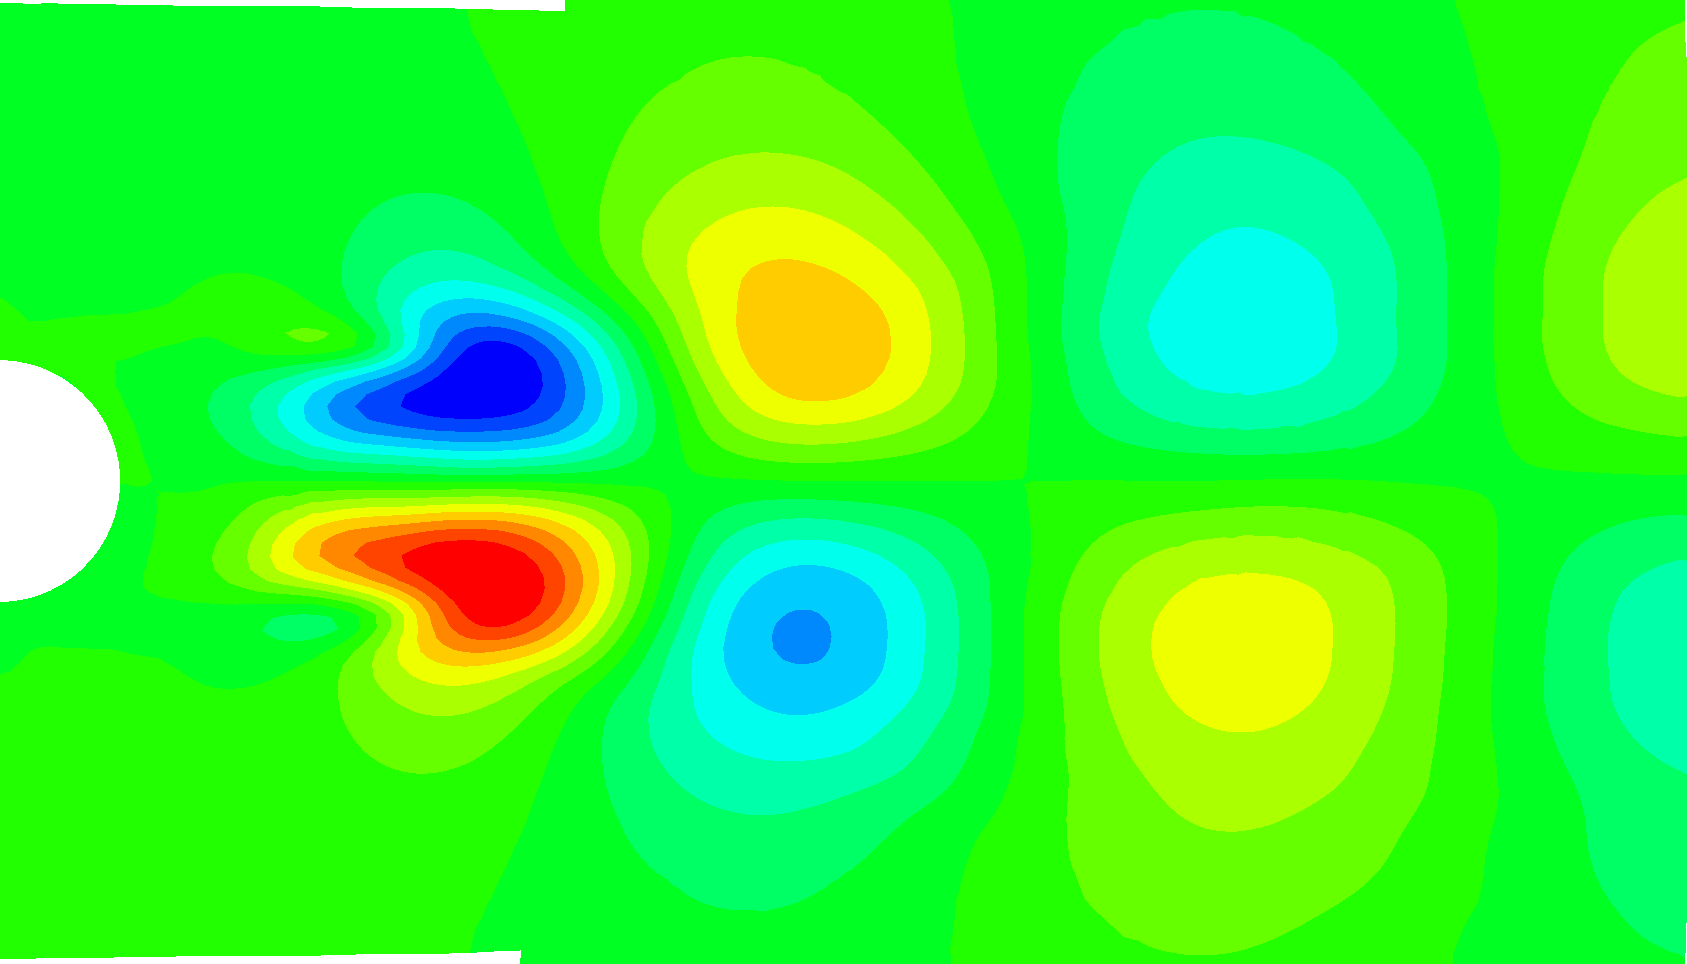
\includegraphics[trim = 0px 0px 0px 0px,clip,width = 0.39\textwidth]{\myImages/res/pom1top1numUx.png}}
	\begin{axis}[
		name = plot1,
		xlabel={$x_r$ [--]},
		ylabel={$y_r$ [--]},
		font = \scriptsize,
		xtick distance=1,ytick distance=1,
		width=\wd\mygraphic,
		height=\ht\mygraphic, %height= 5/3*0.5
		enlargelimits=false,
		scale only axis=true,
		tick align=outside,
		ytick pos=left,
		xtick pos=top,
		% x label style = {at={(axis description cs:3.5,2.5)}},
		x label style = {at={(axis cs:3.5,2.7)}},
		y label style = {at={(axis cs:-1,0)}},
		line width = 1.7pt
		]
		\addplot graphics[xmin=0, xmax=7, ymin=-2, ymax=2,includegraphics={trim = 0px 0px 0px 0px,clip}] {\myImages/res/pom1top1numUx.png};
		\fill [white] (axis cs:0.001,-1.997) rectangle (axis cs:0.5,1.997);
		\fill [black!70](axis cs:0,0) circle [radius=0.5];
		\node at (axis cs:0.22,1.7) {\scriptsize{a)}};
		% \draw [black,dashdotted,line width = 1.3pt] (axis cs:0,0) -- (axis cs:7,0);
		% \node at (axis cs:6.5,1.7) {\scriptsize{PIV}};
		% \node at (axis cs:6.5,-1.7) {\scriptsize{CFD}};
	\end{axis}

	\node [name = osaPsix,anchor = north,at={(plot1.south)},yshift=-0.1cm] {\includegraphics[width=0.39\textwidth]{\myImages/res/psi1_x_scale.png}};
	\node [name = psi0, anchor = north,at={(osaPsix.south)},yshift=0.2cm] {\scriptsize{0}};
	\node [name = psi, anchor = north,at={(psi0.south)},yshift=0.1cm] {\scriptsize{$\bm{\psi}_{1,x},\,_{\mathrm{r}}\bm{\psi}_{1,x}$}};
	\node [name = psiM05, anchor = north west,at={(osaPsix.south west)},yshift=0.2cm] {\scriptsize{negative}};
	\node [name = psiM05, anchor = north east,at={(osaPsix.south east)},yshift=0.2cm] {\scriptsize{positive}};

	% \node [name = psiM05, anchor = center,at={(psi0.center)},xshift=-1.2cm] {positive}};

	\savebox\mygraphic{\includegraphics[trim = 0px 0px 0px 0px,clip,width = 0.39\textwidth]{\myImages/res/pom1top1numRNDpodUx.png}}
	\begin{axis}[
		name = plot2,
		anchor = north,
		at = {(psi.south)},
		yshift = -0.18cm,
		xlabel={$x_r$ [--]},
		ylabel={$y_r$ [--]},
		font = \scriptsize,
		xtick distance=1,ytick distance=1,
		x label style = {at={(axis cs:3.5,-2.7)}},
		y label style = {at={(axis cs:-1,0)}},
		width=\wd\mygraphic,
		height=\ht\mygraphic, %height= 5/3*0.5
		enlargelimits=false,
		scale only axis=true,
		ytick pos=left,
		xtick pos=bottom,
		tick align=outside,
		line width = 1.7pt
		]
		\addplot graphics[xmin=0, xmax=7, ymin=-2, ymax=2,includegraphics={trim = 0px 0px 0px 0px,clip}] {\myImages/res/pom1top1numRNDpodUx.png};
		\fill [white] (axis cs:0.001,-1.997) rectangle (axis cs:0.5,1.997);
		\fill [black!70](axis cs:0,0) circle [radius=0.5];
		\node at (axis cs:0.22,1.7) {\scriptsize{c)}};
		% \draw [black,dashdotted,line width = 1.3pt] (axis cs:0,0) -- (axis cs:7,0);
		% \node [color=white] at (axis cs:6.5,1.7) {\scriptsize{PIV}};
		% \node [color=white] at (axis cs:6.5,-1.7) {\scriptsize{CFD}};
	\end{axis}

	\savebox\mygraphic{\includegraphics[trim = 0px 0px 0px 0px,clip,width = 0.39\textwidth]{\myImages/res/relDiffpodRNDpod.png}}
	\begin{axis}[
		name = plot3,
		xshift = 0.4cm,
		anchor = west,
		at = {(plot1.east)},
		xlabel={$x_r$ [--]},
		ylabel={$y_r$ [--]},
		font = \scriptsize,
		x label style = {at={(axis cs:3.5,2.7)}},
		y label style = {at={(axis cs:8,0)}},
		xtick distance=1,ytick distance=1,
		width=\wd\mygraphic,
		height=\ht\mygraphic, %height= 5/3*0.5
		enlargelimits=false,
		scale only axis=true,
		ytick pos=right,
		xtick pos=top,
		tick align=outside,
		line width = 1.7pt
		]
		\addplot graphics[xmin=0, xmax=7, ymin=-2, ymax=2,includegraphics={trim = 0px 0px 0px 0px,clip}] {\myImages/res/relDiffpodRNDpod.png};
		\fill [white] (axis cs:0.001,-1.997) rectangle (axis cs:0.5,1.997);
		\fill [black!70](axis cs:0,0) circle [radius=0.5];
		\node at (axis cs:0.22,1.7) {\scriptsize{b)}};
		% \draw [black,dashdotted,line width = 1.3pt] (axis cs:0,0) -- (axis cs:7,0);
		% \node [color=white] at (axis cs:6.5,1.7) {\scriptsize{PIV}};
		% \node [color=white] at (axis cs:6.5,-1.7) {\scriptsize{CFD}};
	\end{axis}
	
	\node [name = osaPsix,anchor = north,at={(plot3.south)},yshift=-0.1cm] {\includegraphics[width=0.39\textwidth]{\myImages/res/relDiff_x_scale.png}};
	\node [name = psi0, anchor = north,at={(osaPsix.south)},yshift=0.2cm] {\scriptsize{0 \%}};
	\node [name = psi, anchor = north,at={(psi0.south)},yshift=0.1cm] {\scriptsize{$(\bm{\psi}_{1,x}-\,_{\mathrm{r}}\bm{\psi}_{1,x})/\bm{\psi}_{1,x}$}};
	\node [name = psiM05, anchor = north west,at={(osaPsix.south west)},yshift=0.2cm] {\scriptsize{-0.1 \%}};
	\node [name = psiM05, anchor = north east,at={(osaPsix.south east)},yshift=0.2cm] {\scriptsize{0.1 \%}};

	\begin{axis}[
		name = plot4,
		anchor = west,
		at = {(plot2.east)},
		xshift = 0.4cm,
		xlabel={mode number $j$},
		ylabel={$|\sigma_j - _{\mathrm{r}}\sigma_j|/\sigma_1$ [--]},
		font = \scriptsize,
		% xtick distance=1,ytick distance=1,
		width=\wd\mygraphic,
		height=\ht\mygraphic, %height= 5/3*0.5
		% x label style = {at={(axis cs:3.5,-2.7)}},
		% y label style = {at={(axis cs:-1,0)}},
		enlargelimits=false,
		scale only axis=true,
		ytick pos=right,
		xtick pos=bottom,
		ymode=log,
		line width = 0.85pt,
		xmax=30,
		xmin=0,
		ymin=1e-14,
		ymax=0.1,
		ytick={1e-1,1e-5,1e-10,1e-14}
		% tick align=outside,
		]
		\addplot [color = black,mark =triangle,only marks] table [x expr=\thisrow{x}+1, y expr = \thisrow{scaledWRTSigma1}]{\myGraphs/singValsData/singValsRND_U.dat};
		
		% \addplot [color = red,mark =x,only marks] table [x expr=\thisrow{x}+1, y expr = \thisrow{singVal}]{\myGraphs/singValsData/singValsRND_U.dat};
		% \addplot graphics[xmin=0, xmax=7, ymin=-2, ymax=2,includegraphics={trim = 0px 0px 0px 0px,clip}] {\myImages/res/relDiffpodRNDpod.png};
		% \fill [white] (axis cs:0.001,-1.997) rectangle (axis cs:0.5,1.997);
		% \fill [black!70](axis cs:0,0) circle [radius=0.5];
		% \draw [black,dashdotted,line width = 1.3pt] (axis cs:0,0) -- (axis cs:7,0);
		% \node [color=white] at (axis cs:6.5,1.7) {\scriptsize{PIV}};
		% \node [color=white] at (axis cs:6.5,-1.7) {\scriptsize{CFD}};
	\end{axis}
	\node[anchor=north west] at (plot4.north west) {\scriptsize{d)}};
\end{tikzpicture}

    \includegraphics[width=0.98\textwidth]{02_images/00_export/figure4.png}
    \caption{POD and randomized POD (rPOD) results for simulated velocity field sampled on PoM1. (a) $\bm{\psi}_{1,x}$ computed via POD, (b) relative difference between the POD and rPOD toposes, (c) $_{\mathrm{r}}\bm{\psi}_{1,x}$ computed via rPOD, (d) relative difference between the first 30 POD and rPOD singular values.}
    \label{fig:podRandPODComp}
\end{figure}
In Figures~\ref{fig:podRandPODComp}a and~\ref{fig:podRandPODComp}c, we show the most energetic modes obtained via POD and randomized POD (rPOD) analysis of the simulated velocity data on PoM1, respectively. In Figure~\ref{fig:podRandPODComp}b, the relative error between the two datasets is depicted. Finally, note that the randomized POD variant was performed with $\ell = 30$. In Figure~\ref{fig:podRandPODComp}d, we compare the $\ell$ singular values $\sigma_{\ell}$ obtained via the standard and the randomized POD variant. Altogether, the data depicted in Figure~\ref{fig:podRandPODComp} show that from the point of view of the simulated system analysis, there is no perceivable difference between POD and rPOD.

\section{Results and discussion}
\label{sec:resultsAndDisc}

{In order to statistically validate the numerical model, we first compare time-averaged (mean) velocity and turbulence kinetic energy ($k$) fields as obtained from PIV and CFD.} Next, the turbulence spectra of streamwise and \noteMI{transverse} velocity components in two probe points are compared. At last, the measured and computed data {processed via POD} are analyzed. For each studied mode, the PIV and CFD topos structures and chronos spectra are examined to validate the simulation. {Afterwards, } the results are extended by fully 3D modes obtained by {randomized} POD analysis of the whole numerical dataset from RoI.

\subsection{Mean quantities}
\label{sub:meanData}
The first results to be compared are the mean measured and computed quantities. To obtain the time-averaged data, the equations~\eqref{eq:nsEqs} and~\eqref{eq:kOmegaSSTDES} were first integrated from the initial condition for 10 mean residence times $\tau = (L_{\mathrm{in}} + L_{\mathrm{w}})/u_{\mathrm{in}} \approx {0.13}$ s. Afterwards, the developed flow was simulated for another three seconds while being sampled with the frequency $2\,\mathrm{kHz}$, which is the same frequency, with which the experimental data for POD analysis {have} been sampled. However, in the experiment the mean values {have} been obtained by averaging data from 10 seconds long interval sampled with {the} frequency {of} 100\,Hz.

In the following, we concentrate on the scaled streamwise velocity component $u_r=u/u_{\mathrm{in}}$ and the turbulence kinetic energy $k$ on the planes of measurement PoM1 and PoM2. As in the previous sections, all the spatial coordinates are scaled by the cylinder diameter as $\bm{x}_{r} = (x_{r},y_{r},z_{r}) = \bm{x}/d$. Note that all the spatial coordinates are scaled by the cylinder diameter $d$. Furthermore, corresponding data in all figures are colored utilizing the same scales. {Also, the} {averaged} measured (PIV) and computed (CFD) {data exhibit symmetries with respect to lines}
\begin{equation}
\label{eq:sigmaZeta}
    \begin{array}{rcl}
        \displaystyle \sigma &=& \displaystyle \{(x_{r},y_{r},z_{r})\in\mathbb{R}^{3}:x_{r}\in [0,7],\,y_{r} = 0,z_{r}=0\}\,,\\[0.2cm]
        \displaystyle \zeta  &=& \displaystyle \{(x_{r},y_{r},z_{r})\in\mathbb{R}^{3}:x_{r} = 3.83,\,y_{r}\in [-2,2],z_{r}=0\}\,,
    \end{array}
\end{equation}
depicted in Figure~\ref{fig:meansPom1}a. {To facilitate a qualitative comparison of PIV and simulation, the data in Figures~\ref{fig:meansPom1}~and~\ref{fig:meansPom2} are split, in order, by the lines $\sigma$ and $\zeta$ and the PIV and CFD results are shown side by side.}

\begin{figure}[htbp]
    % \begin{tikzpicture}
	\savebox\mygraphic{\includegraphics[trim = 0px 0px 0px 0px,clip,width = 0.39\textwidth]{\myImages/res/uXMeanComp.png}}
	\begin{axis}[
		name = plot1,
		xlabel={$x_r$ [--]},
		ylabel={$y_r$ [--]},
		font = \scriptsize,
		xtick distance=1,ytick distance=1,
		width=\wd\mygraphic,
		height=\ht\mygraphic, %height= 5/3*0.5
		enlargelimits=false,
		scale only axis=true,
		tick align=outside,
		% x label style = {at={(axis cs:3.5,-2.7)}},
		y label style = {at={(axis cs:-1,0)}},
		ytick pos=left,
		xtick pos=top,
		line width = 1.7pt,
		]
		\addplot graphics[xmin=0, xmax=7, ymin=-2, ymax=2,includegraphics={trim = 0px 0px 0px 0px,clip}] {\myImages/res/uXMeanComp.png};
		\fill [white] (axis cs:0.001,-1.997) rectangle (axis cs:0.5,1.997);
		\fill [black!70](axis cs:0,0) circle [radius=0.5];
		\draw [black,dashdotted,line width = 1pt] (axis cs:0,0) -- (axis cs:7,0);
		\node at (axis cs:6.5,1.7) {\scriptsize{PIV}};
		\node at (axis cs:6.5,-1.7) {\scriptsize{CFD}};
		\draw [black!70,dashed,line width = 1pt] (axis cs:3.83,2) -- (axis cs:3.83,-2);
		\node [black!70] at (axis cs:4.1,1.7) {\scriptsize{$\zeta$}};
		\node  at (axis cs:6.7,0.3) {\scriptsize{$\sigma$}};
		\fill [black](axis cs:4,0) circle [radius=0.1];
		\node  at (axis cs:4.2,-0.3) {\scriptsize{$p_{1}$}};
		\fill [black](axis cs:4.53,1.15) circle [radius=0.1];
		\node  at (axis cs:5,1.15) {\scriptsize{$p_{2}$}};
		\node  at (axis cs:0.25,1.7) {\scriptsize{a)}};
	\end{axis}


	\node [name = osaUx,anchor = south east,at={(plot1.south east)},yshift=-0.7cm] {\includegraphics[width=0.26\textwidth]{\myImages/res/U_x_scale.png}};
	\node [name = ux, anchor = east,at={(osaUx.north west)},yshift=-0.1cm,xshift=-0.1cm] {\scriptsize{$u_r$ [--]}};
	\node [name = psi0, anchor = south,at={(osaUx.north)},yshift=-0.2cm,xshift=-1.61cm] {\scriptsize{-0.2}};
	\node [name = psi0, anchor = west,at={(psi0.east)},xshift=0.22cm] {\scriptsize{0.2}};
	\node [name = psi0, anchor = west,at={(psi0.east)},xshift=0.228cm] {\scriptsize{0.6}};
	\node [name = psi0, anchor = west,at={(psi0.east)},xshift=0.228cm] {\scriptsize{1.0}};
	\node [name = psi0, anchor = west,at={(psi0.east)},xshift=0.02cm] {\scriptsize{1.3}};
	% \node [name = psiM05, anchor = north west,at={(osaPsix.south west)},yshift=0.2cm] {\scriptsize{-0.1 \%}};
	% \node [name = psiM05, anchor = north east,at={(osaPsix.south east)},yshift=0.2cm] {\scriptsize{0.1 \%}};

	\savebox\mygraphic{\includegraphics[trim = 0px 0px 0px 0px,clip,width = 0.39\textwidth]{\myImages/res/kMeanCompV2.png}}
	\begin{axis}[
		name = plot2,
		anchor = west,
		at = {(plot1.east)},
		xshift = 0.3cm,
		xlabel={$x_r$ [--]},
		ylabel={$y_r$ [--]},
		% x label style = {at={(axis cs:3.5,-2.7)}},
		y label style = {at={(axis cs:7.8,0)}},
		font = \scriptsize,
		xtick distance=1,ytick distance=1,
		width=\wd\mygraphic,
		height=\ht\mygraphic, %height= 5/3*0.5
		enlargelimits=false,
		scale only axis=true,
		ytick pos=right,
		xtick pos=top,
		tick align=outside,
		line width = 1.7pt,
		]
		\addplot graphics[xmin=0, xmax=7, ymin=-2, ymax=2,includegraphics={trim = 0px 0px 0px 0px,clip}] {\myImages/res/kMeanCompV2.png};
		\fill [white] (axis cs:0.001,-1.997) rectangle (axis cs:0.5,1.997);
		\fill [black!70](axis cs:0,0) circle [radius=0.5];
		\draw [black,dashdotted,line width = 1.0pt] (axis cs:0,0) -- (axis cs:7,0);
		\node  at (axis cs:6.7,0.3) {\scriptsize{$\sigma$}};
		\node [color=white] at (axis cs:6.5,1.7) {\scriptsize{PIV}};
		\node [color=white] at (axis cs:6.5,-1.7) {\scriptsize{CFD}};
		\node  at (axis cs:0.25,1.7) {\scriptsize{b)}};
	\end{axis}

	\node [name = osak,anchor = south east,at={(plot2.south east)},yshift=-0.7cm,xshift=-0.1cm] {\includegraphics[width=0.26\textwidth]{\myImages/res/k_scale.png}};
	\node [name = k, anchor = east,at={(osak.north west)},yshift=-0.1cm,xshift=-0.1cm] {\scriptsize{$k$ [--]}};
	\node [name = psi0, anchor = south,at={(osak.north)},yshift=-0.2cm,xshift=-1.49cm] {\scriptsize{0.00}};
	\node [name = psi0, anchor = west,at={(psi0.east)},xshift=-0.085cm] {\scriptsize{0.06}};
	\node [name = psi0, anchor = west,at={(psi0.east)},xshift=-0.08cm] {\scriptsize{0.12}};
	\node [name = psi0, anchor = west,at={(psi0.east)},xshift=-0.08cm] {\scriptsize{0.18}};
	\node [name = psi0, anchor = west,at={(psi0.east)},xshift=-0.15cm] {\scriptsize{0.24}};
	\node [name = psi0, anchor = west,at={(psi0.east)},xshift=-0.2cm] {\scriptsize{0.28}};
	% \node [name = psi0, anchor = west,at={(psi0.east)},xshift=0.06cm] {\scriptsize{}};
	% \node [name = psi0, anchor = west,at={(psi0.east)},xshift=0.06cm] {\scriptsize{0.6}};
	% \node [name = psi0, anchor = west,at={(psi0.east)},xshift=0.06cm] {\scriptsize{0.6}};
	% \node [name = psi0, anchor = west,at={(psi0.east)},xshift=0.228cm] {\scriptsize{0.6}};
	% \node [name = psi0, anchor = west,at={(psi0.east)},xshift=0.228cm] {\scriptsize{1.0}};
	% \node [name = psi0, anchor = west,at={(psi0.east)},xshift=0.02cm] {\scriptsize{1.3}};

	\begin{axis}[
		width=0.805\linewidth,
		height = 3cm,
		scale only axis,
		name=plot3,
		anchor = north west,
		at = {(plot1.south west)},
		yshift = -0.8cm,
		xlabel=$x_{r,\sigma}$,
		ylabel={$u_r$ [--]},
		%~ ymode=log,
		%~ xmode=log,
		ymax = 0.8,
		xmin = 0.5,
		ymin = -0.5,
		xmax = 7,
		ytick pos=left,
		font = \scriptsize,
		mark size=4pt,    
		line width = 0.85pt,
		%~ legend style={at={(axis cs:6,2)},anchor=south west},				
	]
	\addplot [color = black,mark =none]table [y=u_x,x =x]{\myGraphs/msIndData/expLineResV1.dat};\label{ux_sigma}
	\addplot [color = red,mark =none]table [y=u_x,x =x]{\myGraphs/msIndData/expLineResV1.dat};\label{expSigm}
	% \addplot [color = blue,mark =none]table [col sep=comma, y expr=(\thisrow{U:0})/5,x expr = {(\thisrow{Points:0})/0.015}]{\myGraphs/msIndData/mS_40p_U.csv};\label{mesh40U}
	% \addplot [color = red,mark =none]table [col sep=comma, y expr=(\thisrow{U:0})/5,x expr = {(\thisrow{Points:0})/0.015}]{\myGraphs/msIndData/mS_50p_U.csv};\label{mesh50U}
	% \addplot [color = green,mark =none]table [col sep=comma, y expr=(\thisrow{U:0})/5,x expr = {(\thisrow{Points:0})/0.015}]{\myGraphs/msIndData/mS_75p_U.csv};\label{mesh70U}
	\addplot [color = blue,mark =none]table [col sep=comma, y expr=(\thisrow{U:0})/5,x expr = {(\thisrow{Points:0})/0.015}]{\myGraphs/msIndData/bCyl_l_3_U.csv};\label{numSigm}
	% \addplot [color = blue,mark =none]table [col sep=comma, y expr=(\thisrow{U:0})/5,x expr = {(\thisrow{Points:0})/0.015}]{\myGraphs/msIndData/u_xprofPOM1.csv};\label{numSigm}
	% \addplot [color = orange,mark =none]table [col sep=comma, y expr=(\thisrow{U:0})/5,x expr = {(\thisrow{Points:0})/0.015}]{\myGraphs/msIndData/mS_120p_U.csv};\label{mesh120U}
	%~ \addplot [color = red,mark =none]table [y=U_x_ms_50_U,x =z_ms_50_U]{\myGraphs/onLineMSV2.dat};\label{mesh50U}
	%~ \addplot [color = green,mark =none]table [y=U_x_ms_70_U,x =z_ms_70_U]{\myGraphs/onLineMSV2.dat};\label{mesh70U}
	%~ \addplot [color = black,mark =none]table [y=U_x_ms_100_U,x =z_ms_100_U]{\myGraphs/onLineMSV2.dat};\label{mesh100U}
	%~ \addplot [color = black,mark =none]table [y=U_x_ms_100_U,x =z_ms_120_U]{\myGraphs/onLineMSV2.dat};\label{mesh100U}
	\coordinate (top) at (rel axis cs:0,1);
	\node  at (axis cs:0.7,0.65) {\scriptsize{c)}};
	\end{axis}
\begin{axis}[
		at = (plot3.north west),
		anchor = north west,
		width=0.805\linewidth,
		height = 3cm,
		scale only axis,
		xlabel=$x_\sigma$,
		%~ ylabel={\textcolor{red}{TKE}},
		ylabel={$k$ [--]},
		%~height=\figHeight,
		scale only axis,
		font = \scriptsize,
		%~ xmin=0,
		%~ xmax=600,
		xmin=0.5,
		xmax=7,
		ymin=0,
		ymax = 0.3,
		%~ ymax=1000,
		hide x axis,
		axis y line*=right,
		line width = 0.85pt,
		%~ axis line style={red},
		%~ axis y label/.append style ={red},
		%~ ytick label/.append style = {red},
		%~ ylabel={$y_{\mathrm{NO}},\,y_{\mathrm{N_{2}O}} \mathrm{\,[ppm]}$},
		mark size=2.5pt, 
	]
	\addplot [color = black,mark =none,dashed]table [y=k,x =x]{\myGraphs/msIndData/expLineResKV1.dat};\label{k_sigma}
	\addplot [color = red,mark =none,dashed]table [y=k,x =x]{\myGraphs/msIndData/expLineResKV1.dat};
	% \addplot [color = blue,mark =none,dashed]table [col sep=comma, y expr=(\thisrow{k}),x expr = {(\thisrow{Points:0})/0.015}]{\myGraphs/msIndData/mS_40p_k.csv};\label{mesh40k}
	% \addplot [color = red,mark =none,dashed]table [col sep=comma, y expr=(\thisrow{k}),x expr = {(\thisrow{Points:0})/0.015}]{\myGraphs/msIndData/mS_50p_k.csv};\label{mesh50k}
	% \addplot [color = green,mark =none,dashed]table [col sep=comma, y expr=(\thisrow{k}),x expr = {(\thisrow{Points:0})/0.015}]{\myGraphs/msIndData/mS_75p_k.csv};\label{mesh70k}
	% \addplot [color = blue,mark =none,dashed]table [col sep=comma, y expr=(\thisrow{k}),x expr = {(\thisrow{Points:0})/0.015}]{\myGraphs/msIndData/bCyl_l_3_k.csv};
	\addplot [color = blue,mark =none,dashed]table [col sep=comma, y expr=(\thisrow{"k"}),x expr = {(\thisrow{"Points:0"})/0.015}]{\myGraphs/msIndData/Znorm_kMean.csv};
	% \addplot [color = orange,mark =none,dashed]table [col sep=comma, y expr=(\thisrow{k}),x expr = {(\thisrow{Points:0})/0.015}]{\myGraphs/msIndData/mS_120p_k.csv};\label{mesh120k}

	\coordinate (bot) at (rel axis cs:1,0);
\end{axis}

\matrix[
	matrix of nodes,
	anchor=north east,
	draw,
	inner sep=0.2em,
	font = \scriptsize,
	%~ thick,
	fill=white,
  ]at([xshift=-0.2cm,yshift=-0.4cm]plot3.north east)
  {
	%~ \ref{100}& CFD old &[5pt]\\
	%~ \ref{60}& XPF - reac, wall&[5pt]\\
	\ref{expSigm}& PIV &
	% \ref{mesh40U}& 40 U &
	% \ref{uxExp}& $U$ exp &[5pt]\\
	% \ref{mesh50U}& 50 U &
	% \ref{mesh70U}& 75 U &
	\ref{ux_sigma}& $u_{r}$ &
	% \ref{mesh120U}& 120 U
	\\
	\ref{numSigm}& CFD &
	% \ref{mesh40k}& 40 k &
	% \ref{uxExp}& $U$ exp &[5pt]\\
	% \ref{mesh50k}& 50 k &
	% \ref{mesh70k}& 75 k &
	\ref{k_sigma}& $k$ &
	% \ref{mesh120k}& 120 k
	\\
%        \ref{legendNoReact}& $\mathrm{thermic\ no\ reaction\ heat}$&[5pt]
	\\};
\end{tikzpicture}
    \includegraphics[width=0.98\textwidth]{02_images/00_export/figure5.png}
    \caption{Measured and computed mean a) streamwise velocity component $u_r$, and b) turbulence kinetic energy $k$ contours on PoM1 with reference points $p_{1}$ and $p_{2}$ for turbulence spectra analysis, c) streamwise velocity component $u_r$ and turbulence kinetic energy $k$ profiles on line $\sigma$.}
    \label{fig:meansPom1}
\end{figure}

\paragraph{PoM1}
As depicted in Figure~\ref{fig:meansPom1}a, there is a good qualitative agreement between the experiment and simulation comparing mean measured and calculated velocity contours on the PoM1. Both PIV and CFD velocity fields comprise recirculation zone in the near-wake directly behind the cylinder and ending approximately at $x_{{r}} = 2$. Furthermore, the simulated and the measured wake dimensions are roughly equal. However, compared to the measured mean velocity field, the simulation estimates a slightly more pronounced recirculation zone and a slightly bigger wake, albeit with a less apparent velocity deficiency.

A similar information as from the comparison of {the} streamwise velocity may be gathered from the {$k$} distribution {shown} in Figure~\ref{fig:meansPom1}b. Namely, in both the experiment and simulation, there is a region of low turbulence kinetic energy right behind the cylinder and a local {$k$} maximum close to the {$\sigma$ line (test-section plane of symmetry)} at $x_r \approx 2.5$. Still, the simulated $k$ is lower than the measured one. Moreover, the computed low-$k$ region right behind the cylinder is smaller and not bounded by high-$k$ bands, cf. {top and bottom parts of} Figure~\ref{fig:meansPom1}b at $x_r\approx 1$. 

Finally to compare {the} measured and simulated results quantitatively, {in Figure~\ref{fig:meansPom1}c,} we plot the streamwise velocity component $u_r$ and the turbulence kinetic energy $k$ along the line $\sigma$. The local measured mean velocity minimum is placed at $x_r\doteq 1.57$ and has the value of $\mathrm{min}(u_{r,\mathrm{exp}}^{\sigma})\doteq -0.18$. The computed local velocity minimum is $\mathrm{min}(u_{\mathrm{sim}}^{\sigma})\doteq -0.33$ and it is placed at $x_r\doteq 1.61$. With respect to the ranges of the measured data, the relative difference between the experiment and simulation is $\Delta u_{r,\mathrm{min}}^{\sigma} = 16\,\%$ and $\Delta x_{r,\mathrm{min}} = 0.6\,\%$. %The average relative error in $u_r$ on $\sigma$ is $1.2\,\%$.

The situation with the turbulence kinetic energy {quantitative} mean results on line $\sigma$ is similar to the streamwise velocity component. Overall, the simulation under-estimates the amount of $k$ in the system. % by approximately $12\,\%$.At the same time, for $x_r\in [0.5,1.5]$, the computed $k$ seems to be actually over-estimated by roughly $27\,\%$, which is observable even via a comparison of the qualitative results in Figure~\ref{fig:meansPom1}. 
Also, similarly to the case of $u_{{r}}$, the biggest discrepancy in the data is encountered for the local $k$ maximum observed at $x_r\doteq 2.28$ in experiment and at $x_r\doteq 2.22$ in simulation (relative error of $2.6\,\%$) with the respective $k$ values of $0.28$ and $0.24$ (relative error of $14\,\%$).

\begin{figure}[htbp]
    % \begin{tikzpicture}
	\savebox\mygraphic{\includegraphics[trim = 0px 0px 0px 0px,clip,width = 0.39\textwidth]{\myImages/res/uXMeanCompPOM2V2.png}}
	\begin{axis}[
		name = plot1,
		xlabel={$z_r$ [--]},
		ylabel={$y_r$ [--]},
		font = \scriptsize,
		xtick distance=1,ytick distance=1,
		width=\wd\mygraphic,
		height=\ht\mygraphic, %height= 5/3*0.5
		enlargelimits=false,
		scale only axis=true,
		tick align=outside,
		ytick pos=left,
		xtick pos=top,
		y label style = {at={(axis cs:-3.6,0)}},
		% x label style = {at={(axis cs:0,-2.7)}},
		line width = 1.7pt
		]
		\addplot graphics[xmin=-3, xmax=3, ymin=-2, ymax=2,includegraphics={trim = 0px 0px 0px 0px,clip}] {\myImages/res/uXMeanCompPOM2V2.png};
		% \fill [white] (axis cs:0.001,-1.997) rectangle (axis cs:0.5,1.997);
		% \fill [black!70](axis cs:0,0) circle [radius=0.5];
		% \draw [black,dashdotted,line width = 1.0pt] (axis cs:-2,0) -- (axis cs:2,0);
		\draw [black!70,dashed,line width = 1.0pt] (axis cs:0,2) -- (axis cs:0,-2);
		\node [white] at (axis cs:0.2,1.7) {\scriptsize{$\zeta$}};
		\node [white] at (axis cs:-2.55,1.75) {\scriptsize{PIV}};
		\node [white] at (axis cs:-2.7,0) {\scriptsize{a)}};
		\node [white] at (axis cs:2.55,1.75) {\scriptsize{CFD}};
	\end{axis}
	\node [name = osaUx,anchor = south east,at={(plot1.south east)},yshift=-0.7cm] {\includegraphics[width=0.26\textwidth]{\myImages/res/U_x_scale2.png}};
	\node [name = ux, anchor = east,at={(osaUx.north west)},yshift=-0.1cm,xshift=-0.1cm] {\scriptsize{$u_r$ [--]}};
	\node [name = psi0, anchor = south,at={(osaUx.north)},yshift=-0.2cm,xshift=-1.6cm] {\scriptsize{\ 0.7}};
	\node [name = psi0, anchor = west,at={(psi0.east)},xshift=0.45cm] {\scriptsize{0.8}};
	\node [name = psi0, anchor = west,at={(psi0.east)},xshift=0.45cm] {\scriptsize{0.9}};
	\node [name = psi0, anchor = west,at={(psi0.east)},xshift=0.45cm] {\scriptsize{1.0}};
	% \node [name = psi0, anchor = west,at={(psi0.east)},xshift=-0.11cm] {\scriptsize{0.98}};
	% \node [name = psi0, anchor = west,at={(psi0.east)},xshift=-0.14cm] {\scriptsize{1.02}};

	\savebox\mygraphic{\includegraphics[trim = 0px 0px 0px 0px,clip,width = 0.39\textwidth]{\myImages/res/kMeanCompPOM2.png}}
	\begin{axis}[
		name = plot2,
		anchor = west,
		at = {(plot1.east)},
		xshift = 0.4cm,
		xlabel={$z_r$ [--]},
		ylabel={$y_r$ [--]},
		% x label style = {at={(axis cs:0,-2.7)}},
		y label style = {at={(axis cs:3.5,0)}},
		font = \scriptsize,
		xtick distance=1,ytick distance=1,
		width=\wd\mygraphic,
		height=\ht\mygraphic, %height= 5/3*0.5
		enlargelimits=false,
		scale only axis=true,
		tick align=outside,
		ytick pos=right,
		xtick pos=top,
		line width = 1.7pt
		]
		\addplot graphics[xmin=-3, xmax=3, ymin=-2, ymax=2,includegraphics={trim = 0px 0px 0px 0px,clip}] {\myImages/res/kMeanCompPOM2.png};
		% \fill [white] (axis cs:0.001,-1.997) rectangle (axis cs:0.5,1.997);
		% \fill [black!70](axis cs:0,0) circle [radius=0.5];
		% \draw [black,dashdotted,line width = 1.0pt] (axis cs:-2,0) -- (axis cs:2,0);
		\draw [black!70,dashed,line width = 1.0pt] (axis cs:0,2) -- (axis cs:0,-2);
		\node [white] at (axis cs:0.2,1.7) {\scriptsize{$\zeta$}};
		\node [white] at (axis cs:-2.55,1.75) {\scriptsize{PIV}};
		\node [white] at (axis cs:2.55,1.75) {\scriptsize{CFD}};
		\node [black] at (axis cs:-2.7,0) {\scriptsize{b)}};
	\end{axis}
	\node [name = osak,anchor = south east,at={(plot2.south east)},yshift=-0.7cm,xshift=0.1cm] {\includegraphics[width=0.26\textwidth]{\myImages/res/k_scale2.png}};
	\node [name = k, anchor = east,at={(osak.north west)},yshift=-0.1cm,xshift=-0.1cm] {\scriptsize{$k$ [--]}};
	\node [name = psi0, anchor = south,at={(osak.north)},yshift=-0.2cm,xshift=-1.49cm] {\scriptsize{0.00}};
	\node [name = psi0, anchor = west,at={(psi0.east)},xshift=0.03cm] {\scriptsize{0.04}};
	\node [name = psi0, anchor = west,at={(psi0.east)},xshift=0.03cm] {\scriptsize{0.08}};
	\node [name = psi0, anchor = west,at={(psi0.east)},xshift=0.03cm] {\scriptsize{0.12}};
	\node [name = psi0, anchor = west,at={(psi0.east)},xshift=0.03cm] {\scriptsize{0.15}};
	% \node [name = psi0, anchor = west,at={(psi0.east)},xshift=-0.2cm] {\scriptsize{0.28}};

	\begin{axis}[
		width=0.815\linewidth,
		height = 3cm,
		yshift = -0.8cm,
		scale only axis,
		name=plot3,
		at = (plot1.south west),
		anchor = north west,
		font = \scriptsize,
		xlabel={$y_{r,\zeta}$ [--]},
		ylabel={$u_r$ [--]},
		% yticklabels={0,0.05,0.1,0.15},
		% yticklabel style={
		% 	/pgf/number format/.cd, fixed, fixed zerofill,
		% 	/pgf/number format/precision=2,
		% 	/pgf/number format/fixed},
		%~ ymode=log,
		%~ xmode=log,
		% ymax = 0.8,
		xmin = -2,
		% ymin = -0.5,
		xmax = 2,
		ytick pos=left,
		mark size=4pt,    
		line width = 0.85pt,
		%~ legend style={at={(axis cs:6,2)},anchor=south west},				
	]
	% \addplot [color = black!50,mark =none]table [y=u_x,x =x]{\myGraphs/msIndData/expLineResV1.dat};\label{expSigm}
	% \addplot [color = blue,mark =none]table [col sep=comma, y expr=(\thisrow{U:0})/5,x expr = {(\thisrow{Points:0})/0.015}]{\myGraphs/msIndData/mS_40p_U.csv};\label{mesh40U}
	% \addplot [color = red,mark =none]table [col sep=comma, y expr=(\thisrow{U:0})/5,x expr = {(\thisrow{Points:0})/0.015}]{\myGraphs/msIndData/mS_50p_U.csv};\label{mesh50U}
	% \addplot [color = green,mark =none]table [col sep=comma, y expr=(\thisrow{U:0})/5,x expr = {(\thisrow{Points:0})/0.015}]{\myGraphs/msIndData/mS_75p_U.csv};\label{mesh70U}
	\addplot [color = blue,mark =none]table [col sep=comma, y expr=(\thisrow{U:0})/5,x expr = {(\thisrow{Points:1})/0.015}]{\myGraphs/msIndData/bCyl_l_3Ver_U.csv};
	\addplot [color = red,mark =none]table [col sep=comma, y expr=(\thisrow{W[m_s]})/5,x expr = {(\thisrow{Points:1}-30.0)/15}]{\myGraphs/msIndData/POM2.csv};
	% \addplot [color = orange,mark =none]table [col sep=comma, y expr=(\thisrow{U:0})/5,x expr = {(\thisrow{Points:0})/0.015}]{\myGraphs/msIndData/mS_120p_U.csv};\label{mesh120U}
	%~ \addplot [color = red,mark =none]table [y=U_x_ms_50_U,x =z_ms_50_U]{\myGraphs/onLineMSV2.dat};\label{mesh50U}
	%~ \addplot [color = green,mark =none]table [y=U_x_ms_70_U,x =z_ms_70_U]{\myGraphs/onLineMSV2.dat};\label{mesh70U}
	%~ \addplot [color = black,mark =none]table [y=U_x_ms_100_U,x =z_ms_100_U]{\myGraphs/onLineMSV2.dat};\label{mesh100U}
	%~ \addplot [color = black,mark =none]table [y=U_x_ms_100_U,x =z_ms_120_U]{\myGraphs/onLineMSV2.dat};\label{mesh100U}
	\coordinate (top) at (rel axis cs:0,1);
	\end{axis}
	\node [name = c, anchor = west,at={(plot3.west)},yshift=-0.0cm,xshift=-0.0cm] {\scriptsize{c)}};
\begin{axis}[
		at = (plot3.north west),
		anchor = north west,
		width=0.815\linewidth,
		height = 3cm,
		scale only axis,
		xlabel={$x_\sigma$ [--]},
		%~ ylabel={\textcolor{red}{TKE}},
		ylabel={$k$ [--]},
		%~height=\figHeight,
		scale only axis,
		%~ xmin=0,
		%~ xmax=600,
		% yticklabels={0,0.05,0.1,0.15},
					yticklabel style={
			/pgf/number format/.cd, fixed, fixed zerofill,
			/pgf/number format/precision=2,
			/pgf/number format/fixed},
		xmin=-2,
		xmax=2,
		ymin=0,
		% ymax = 0.3,
		%~ ymax=1000,
		hide x axis,
		axis y line*=right,
		font=\scriptsize,
		line width = 0.85pt,
		%~ axis line style={red},
		%~ axis y label/.append style ={red},
		%~ ytick label/.append style = {red},
		%~ ylabel={$y_{\mathrm{NO}},\,y_{\mathrm{N_{2}O}} \mathrm{\,[ppm]}$},
		mark size=2.5pt, 
	]
	% \addplot [color = black!50,mark =none,dashed]table [y=k,x =x]{\myGraphs/msIndData/expLineResKV1.dat};\label{1expSigmK}
	% \addplot [color = blue,mark =none,dashed]table [col sep=comma, y expr=(\thisrow{k}),x expr = {(\thisrow{Points:0})/0.015}]{\myGraphs/msIndData/mS_40p_k.csv};\label{mesh40k}
	% \addplot [color = red,mark =none,dashed]table [col sep=comma, y expr=(\thisrow{k}),x expr = {(\thisrow{Points:0})/0.015}]{\myGraphs/msIndData/mS_50p_k.csv};\label{mesh50k}
	% \addplot [color = green,mark =none,dashed]table [col sep=comma, y expr=(\thisrow{k}),x expr = {(\thisrow{Points:0})/0.015}]{\myGraphs/msIndData/mS_75p_k.csv};\label{mesh70k}
	\addplot [color = red,mark =none,dashed]table [col sep=comma, y expr=(\thisrow{Result})*10,x expr = {(\thisrow{Points:1}-30.0)/15}]{\myGraphs/msIndData/POM2.csv};
	\addplot [color = blue,mark =none,dashed]table [col sep=comma, y expr=(\thisrow{k}),x expr = {(\thisrow{Points:1})/0.015}]{\myGraphs/msIndData/bCyl_l_3Ver_k.csv};
	% \addplot [color = orange,mark =none,dashed]table [col sep=comma, y expr=(\thisrow{k}),x expr = {(\thisrow{Points:0})/0.015}]{\myGraphs/msIndData/mS_120p_k.csv};\label{mesh120k}

	\coordinate (bot) at (rel axis cs:1,0);
\end{axis}
\matrix[
	matrix of nodes,
	anchor=south east,
	draw,
	inner sep=0.2em,
	font = \scriptsize,
	%~ thick,
	fill=white,
  ]at([xshift=-0.2cm,yshift=0.2cm]plot3.south east)
  {
	%~ \ref{100}& CFD old &[5pt]\\
	%~ \ref{60}& XPF - reac, wall&[5pt]\\
	\ref{expSigm}& PIV &
	% \ref{mesh40U}& 40 U &
	% \ref{uxExp}& $U$ exp &[5pt]\\
	% \ref{mesh50U}& 50 U &
	% \ref{mesh70U}& 75 U &
	\ref{ux_sigma}& $u_{x,r}$ &
	% \ref{mesh120U}& 120 U
	\\
	\ref{numSigm}& CFD &
	% \ref{mesh40k}& 40 k &
	% \ref{uxExp}& $U$ exp &[5pt]\\
	% \ref{mesh50k}& 50 k &
	% \ref{mesh70k}& 75 k &
	\ref{k_sigma}& $k$ &
	% \ref{mesh120k}& 120 k
	\\
%        \ref{legendNoReact}& $\mathrm{thermic\ no\ reaction\ heat}$&[5pt]
	\\};
%     \matrix[
%         matrix of nodes,
%         anchor=center,
%         draw,
% 		font = \scriptsize,
%         inner sep=0.2em,
%         %~ thick,
%         fill=white,
%       ]at([xshift=-0.2cm,yshift=-0.0cm]plot2.center)
%       {
%         %~ \ref{100}& CFD old &[5pt]\\
%         %~ \ref{60}& XPF - reac, wall&[5pt]\\
% 		\ref{expSigm}& PIV &
%         % \ref{mesh40U}& 40 U &
%         % \ref{uxExp}& $U$ exp &[5pt]\\
%         % \ref{mesh50U}& 50 U &
%         % \ref{mesh70U}& 75 U &
%         \ref{numSigm}& $u_{x,r}$ &
%         % \ref{mesh120U}& 120 U
% 		\\
% 		\ref{numSigm}& CFD &
%         % \ref{mesh40k}& 40 k &
%         % \ref{uxExp}& $U$ exp &[5pt]\\
%         % \ref{mesh50k}& 50 k &
%         % \ref{mesh70k}& 75 k &
%         \ref{expSigmK}& $k$ &
%         % \ref{mesh120k}& 120 k
% 		\\
% %        \ref{legendNoReact}& $\mathrm{thermic\ no\ reaction\ heat}$&[5pt]
%         \\};

\end{tikzpicture}
    \includegraphics[width=0.98\textwidth]{02_images/00_export/figure6.png}
    \caption{Measured and computed time-averaged a) stream-wise velocity component, and b) turbulence kinetic energy contours on PoM2, c) stream-wise velocity component and turbulence kinetic energy profile on line $\zeta$.}
    \label{fig:meansPom2}
\end{figure}

\paragraph{PoM2}
As shown in Figure~\ref{fig:meansPom2}a-b, the measured and computed streamwise velocity component $u_r$ and turbulence kinetic energy $k$ contours provide {a} relatively good compliance {also on the PoM2}. Similarly as in the case of the PoM1, the simulated wake dimension is under-estimated in comparison with the experiment. Particularly, the measured and computed wakes are, in order, approximately $W_{\mathrm{exp}}^{y_{r}} \doteq$ 1.5 and $W_{\mathrm{num}}^{y_{r}} \doteq$ 1.25 wide. Additionally, considering {the} streamwise velocity component profile on line $\zeta$ {plotted} in Figure~\ref{fig:meansPom2}c, note that the minimum is located directly behind the cylinder and its value is almost {the} same for both {the} PIV and CFD data, $\mathrm{min}(u_{r,\mathrm{exp}}^{\zeta}) \doteq \mathrm{min}(u_{r,\mathrm{num}}^{\zeta})\doteq 0.17 $.

On the other hand, {upon comparison of} PIV and CFD {$k$} profiles on {the} $\zeta$ line {given} in Figure~\ref{fig:meansPom2}c, {it may be noted} that the simulated $k$ profile {is, in the vicinity of its} maximum ($y_r\in$ [-0.5, 0.5]){,} {flatter than its measured counterpart}. Consequently, the measured maximal value of $k$ is $\mathrm{max}(k_{\mathrm{exp}}^{\zeta})\doteq 0.17$, while the simulation {estimates} $\mathrm{max}(k_{\mathrm{num}}^{\zeta})\doteq 0.14$ (relative error of $18\,\%$).

Despite the quantitative discrepancies in the data, all the qualitative trends in the time-averaged variables are in agreement. Furthermore, the quantitative discrepancies between the PIV and CFD data are similar or lower than the ones reported {in the relevant literature, see }for example \citep{wen2016,gonzalez2019} or \citep{mustafa2021}.

\begin{figure}[htbp]
    \centering
    % \begin{tikzpicture}
	\begin{axis}[
			width=0.37\textwidth,
			height = 0.27\textwidth,
			scale only axis,
			name=plot1,
			xlabel={$f$ [Hz]},
			ylabel={$E$ [a.u]},
			ymode=log,
			xmode=log,
			ymax = 100,
			xmin = 1,
			ymin = 1e-4,
			xmax=1e3,
			ytick pos=left,
			font=\scriptsize,
			mark size=4pt,    
			ytick={100,1,0.01,0.0001},
			% legend style={at={(axis cs:1.5,1e-1)},anchor=north west},
			legend style={anchor=south west},
			legend pos=south west,
			smooth,
			xtick pos=top,			
			line width = 0.85pt
		]
		\addplot [color = blue,mark =none]table [y expr=(\thisrow{ux}),x=x]{\myGraphs/spctraData/point0_probeSpectraExp.dat};
		\addlegendentry{$u$}
		\addplot [color = green!70!black,mark =none]table [y expr=(\thisrow{uy})*1,x=x]{\myGraphs/spctraData/point0_probeSpectraExp.dat};
		\addlegendentry{$v$}
		\addplot [color=red,mark=none] coordinates {
			(71,26.282891182634373)
			(333,2 )
		};
		\addlegendentry{Kolm.}
		\addplot [color=orange,mark=none] coordinates {
			(333,2)
			(1e3,0.07385207399999995)
		};
		\addlegendentry{Kraich.}
		\addplot [color=black,mark=none,solid] coordinates {
			(71, 1e-4)
			(71, 1e2)
		};
		\addplot [color=black,mark=none,dashed] coordinates {
			(142, 1e-4)
			(142, 1e2)
		};
		\addplot [color=black,mark=none,dashdotted] coordinates {
			(213, 1e-4)
			(213, 1e2)
		};
		\node[above left,anchor=east,black] at (axis cs:71,5e-4) {$f_{1}$};
		\node[above left,anchor=east,black] at (axis cs:162,5e-4) {$f_{2}$};
		\node[above right,anchor=west,black] at (axis cs:213,5e-4) {$f_{3}$};
		\draw (axis cs:250,3.225054343350042) -- (axis cs:300,3.225054343350042)--(axis cs:300,2.379952523639248);
		\node[above,xshift=0.2cm,yshift=-0.1cm] at (axis cs:300,3.225054343350042) {\scriptsize{-5/3}};

		\draw (axis cs:600,0.34190775000000023) -- (axis cs:720,0.34190775000000023)--(axis cs:720,0.19786328124999977);
		\node[above] at (axis cs:720,0.34190775000000023) {\scriptsize{-3}};
	\end{axis}
	\node[at={(plot1.north west)},anchor=north west] {\small{PIV $p_{1}$}};
	\begin{axis}[
			width=0.37\textwidth,
			height = 0.27\textwidth,
			scale only axis,
			xshift=0.4cm,
			font=\scriptsize,
			name=plot2,
			at={(plot1.east)},
			anchor=west,
			xlabel={$f$ [Hz]},
			ylabel={$E$ [a.u]},
			ymode=log,
			xmode=log,
			ymax = 100,
			xmin = 1,
			ytick pos=right,
			xtick pos=top,
			ymin = 1e-4,
			ytick={100,1,0.01,0.0001},
			xmax=1e3,
			% ytick pos=left,
			mark size=4pt,    
			legend style={anchor=south west},
			legend pos=south west,
			smooth,
			line width = 0.85pt
		]
		\addplot [color = blue,mark =none]table [y expr=(\thisrow{ux}),x=x]{\myGraphs/spctraData/point1_probeSpectraExp.dat};
		\addlegendentry{$u$}
		\addplot [color = green!70!black,mark =none]table [y expr=(\thisrow{uy})*1,x=x]{\myGraphs/spctraData/point1_probeSpectraExp.dat};
		\addlegendentry{$v$}
		% \addplot [color=red,mark=none] coordinates {
		% 	(213,13.16337723958297)
		% 	(1e3,0.9999999999999994 )
		% };
		% \addlegendentry{Kolm.}
		% \addplot [color=orange,mark=none] coordinates {
		% 	(213,13.16337723958297)
		% 	(1e3,0.12717293651999992 )
		% };
		% \addlegendentry{Kraich.}
		\addplot [color=red,mark=none] coordinates {
			(71,26.282891182634373)
			(333,2 )
		};
		\addlegendentry{Kolm.}
		\addplot [color=orange,mark=none] coordinates {
			(333,2)
			(1e3,0.07385207399999995)
		};
		\addlegendentry{Kraich.}
		\addplot [color=black,mark=none,solid] coordinates {
			(71, 1e-4)
			(71, 1e2)
		};
		\addplot [color=black,mark=none,dashed] coordinates {
			(142, 1e-4)
			(142, 1e2)
		};
		\addplot [color=black,mark=none,dashdotted] coordinates {
			(213, 1e-4)
			(213, 1e2)
		};
		\node[above left,anchor=east,black] at (axis cs:71,5e-4) {$f_{1}$};
		\node[above left,anchor=east,black] at (axis cs:162,5e-4) {$f_{2}$};
		\node[above right,anchor=west,black] at (axis cs:213,5e-4) {$f_{3}$};

		% \draw (axis cs:400,1.9870771331249972 ) -- (axis cs:400,1.39)--(axis cs:450,1.39);
		% \node[below] at (axis cs:400,1.39) {\scriptsize{-3}};

		% \draw (axis cs:450,3.783) -- (axis cs:530,3.783)--(axis cs:530,2.880240673477308);
		% \node[above] at (axis cs:500,3.783) {\scriptsize{-5/3}};
		\draw (axis cs:250,3.225054343350042) -- (axis cs:300,3.225054343350042)--(axis cs:300,2.379952523639248);
		\node[above,xshift=0.2cm,yshift=-0.1cm] at (axis cs:300,3.225054343350042) {\scriptsize{-5/3}};

		\draw (axis cs:600,0.34190775000000023) -- (axis cs:720,0.34190775000000023)--(axis cs:720,0.19786328124999977);
		\node[above] at (axis cs:720,0.34190775000000023) {\scriptsize{-3}};
	\end{axis}
	\node[at={(plot2.north west)},anchor=north west] {\small{PIV $p_{2}$}};

	\begin{axis}[
			width=0.37\textwidth,
			height = 0.27\textwidth,
			scale only axis,
			yshift=-0.3cm,
			font=\scriptsize,
			name=plot3,
			at={(plot1.south)},
			anchor=north,
			xlabel={$f$ [Hz]},
			ylabel={$E$ [a.u]},
			ymode=log,
			xmode=log,
			ymax = 100,
			ytick={100,1,0.01,0.0001},
			xmin = 1,
			ytick pos=left,
			xtick pos=bottom,
			ymin = 1e-4,
			xmax=1e3,
			% ytick pos=left,
			mark size=4pt,    
			legend style={anchor=south west},
			legend pos=south west,
			smooth,
			line width = 0.85pt
		]
		\addplot [color = blue,mark =none]table [y expr=\thisrow{ux}^2,x=x]{\myGraphs/spctraData/point0_probeSpectra.dat};
		\addlegendentry{$u$}
		\addplot [color = green!70!black,mark =none]table [y expr=\thisrow{uy}^2,x=x]{\myGraphs/spctraData/point0_probeSpectra.dat};
		\addlegendentry{$v$}
		\addplot [color=red,mark=none] coordinates {
			(71,26.282891182634373)
			(333,2 )
		};
		\addlegendentry{Kolm.}
		\addplot [color=orange,mark=none] coordinates {
			(333,2)
			(1e3,0.07385207399999995)
		};
		\addlegendentry{Kraich.}
		\addplot [color=black,mark=none,solid] coordinates {
			(71, 1e-4)
			(71, 1e2)
		};
		\addplot [color=black,mark=none,dashed] coordinates {
			(142, 1e-4)
			(142, 1e2)
		};
		\addplot [color=black,mark=none,dashdotted] coordinates {
			(213, 1e-4)
			(213, 1e2)
		};
		\node[above left,anchor=east,black] at (axis cs:71,5e-4) {$f_{1}$};
		\node[above left,anchor=east,black] at (axis cs:162,5e-4) {$f_{2}$};
		\node[above right,anchor=west,black] at (axis cs:213,5e-4) {$f_{3}$};


		\draw (axis cs:250,3.225054343350042) -- (axis cs:300,3.225054343350042)--(axis cs:300,2.379952523639248);
		\node[above,xshift=0.2cm,yshift=-0.1cm] at (axis cs:300,3.225054343350042) {\scriptsize{-5/3}};

		\draw (axis cs:600,0.34190775000000023) -- (axis cs:720,0.34190775000000023)--(axis cs:720,0.19786328124999977);
		\node[above] at (axis cs:720,0.34190775000000023) {\scriptsize{-3}};
	\end{axis}
	\node[at={(plot3.north west)},anchor=north west] {\small{CFD $p_{1}$}};

	\begin{axis}[
			width=0.37\textwidth,
			height = 0.27\textwidth,
			scale only axis,
			xshift=0.4cm,
			font=\scriptsize,
			name=plot4,
			at={(plot3.east)},
			anchor=west,
			xlabel={$f$ [Hz]},
			ylabel={$E$ [a.u]},
			ytick={100,1,0.01,0.0001},
			ymode=log,
			xmode=log,
			ymax = 100,
			xmin = 1,
			ytick pos=right,
			xtick pos=bottom,
			ymin = 1e-4,
			xmax=1e3,
			% ytick pos=left,
			mark size=4pt,    
			legend style={anchor=south west},
			legend pos=south west,
			smooth,
			line width = 0.85pt
		]
		\addplot [color = blue,mark =none]table [y expr=\thisrow{ux}^2,x=x]{\myGraphs/spctraData/point1_probeSpectra.dat};
		\addlegendentry{$u$}
		\addplot [color = green!70!black,mark =none]table [y expr=\thisrow{uy}^2,x=x]{\myGraphs/spctraData/point1_probeSpectra.dat};
		\addlegendentry{$v$}
		\addplot [color=red,mark=none] coordinates {
			(71,26.282891182634373)
			(333,2 )
		};
		\addlegendentry{Kolm.}
		\addplot [color=orange,mark=none] coordinates {
			(333,2)
			(1e3,0.07385207399999995)
		};
		\addlegendentry{Kraich.}
		\addplot [color=black,mark=none,solid] coordinates {
			(71, 1e-4)
			(71, 1e2)
		};
		\addplot [color=black,mark=none,dashed] coordinates {
			(142, 1e-4)
			(142, 1e2)
		};
		\addplot [color=black,mark=none,dashdotted] coordinates {
			(213, 1e-4)
			(213, 1e2)
		};
		\node[above left,anchor=east,black] at (axis cs:71,5e-4) {$f_{1}$};
		\node[above left,anchor=east,black] at (axis cs:162,5e-4) {$f_{2}$};
		\node[above right,anchor=west,black] at (axis cs:213,5e-4) {$f_{3}$};

		\draw (axis cs:250,3.225054343350042) -- (axis cs:300,3.225054343350042)--(axis cs:300,2.379952523639248);
		\node[above,xshift=0.2cm,yshift=-0.1cm] at (axis cs:300,3.225054343350042) {\scriptsize{-5/3}};

		\draw (axis cs:600,0.34190775000000023) -- (axis cs:720,0.34190775000000023)--(axis cs:720,0.19786328124999977);
		\node[above] at (axis cs:720,0.34190775000000023) {\scriptsize{-3}};
	\end{axis}
	\node[at={(plot4.north west)},anchor=north west] {\small{CFD $p_{2}$}};
\end{tikzpicture}
    \includegraphics[width=0.98\textwidth]{02_images/00_export/figure7.png}
    \caption{Comparison of measured and computed turbulence spectra in probe points $p_{1}$ and $p_{2}$.}
    \label{fig:turbSpectraPts}
\end{figure}

\subsection{Turbulence spectra}
\label{sub:turbSpectra}

The initial comparison of measured and computed flow dynamics is performed utilizing the spectra of streamwise and \noteMI{transverse} velocity components evaluated in the points $p_{1}$ and $p_{2}$ depicted in Figure~\ref{fig:meansPom1} and located at $(4,0,0)$ and $(4.53,1.15,0)$, respectively. The measured and computed spectra are shown in Figure~\ref{fig:turbSpectraPts}. Similarly to \citep{uruba2020a}, all the results were processed using {a} standard method with the Hamming window.

In all the graphs in Figure~\ref{fig:turbSpectraPts}, we added vertical lines representing the frequencies of the three most important {flow} harmonics. All the shown vertical lines, i.e. for both the experiment and simulation, are placed at the same positions. Namely, the fundamental harmonic $f_{1} = 71\,\mathrm{Hz}$ corresponds to the Strouhal number $\Strou = f_{1}\,d/u_{\mathrm{in}} = 0.21\approx 0.2$, which is a typical value of $\Strou$ in the broad range of Reynolds numbers starting with $\Rey \gtrapprox 200$, see e.g. \citep{lienhard1966} and references therein.

The higher harmonics are located at $f_{2} = 142\,\mathrm{Hz}$ and $f_{3} = 213\,\mathrm{Hz}$, respectively. All the three harmonics may be identified in both the measured and computed spectra. Furthermore, all the spectra contain an observable decay in turbulent energy \noteMI{that consists of two parts with slopes $-5/3$ and $-3$, respectively. This type of spectra can be identified according to the two-dimensional turbulence theory, see \citep{kraichnan1967,rutgers1998}. \noteMI{The $E(f)\sim f^{-5/3}$ part of the spectrum represents the inverse energy cascade towards bigger scales with zero enstrophy flow, while the $E(f)\sim f^{-3}$ part represents the upward enstrophy flow with zero-energy flow \citep{kraichnan1967,rose1978}}. The two regions are separated by the scale on \noteMI{which the energy and enstrophy are injected into the system} \citep{rose1978}. For the studied flow, the energy-injection scale approximately corresponds to $f_{\mathrm{in}} = u_{\mathrm{in}}/d = 333\,$Hz.}

% URUBA: This energy-injection scale corresponds to $f_{2}$ and $f_{3}$ for $u$ and $v$, respectively. <- MI: I am not sure that I agree with this. the change in slope is substantially later that at f_{2} or f_{3}

\begin{figure}[htbp]
    \centering
    % \begin{tikzpicture}
	\begin{axis}[
			width=0.8\linewidth,
			height = 4cm,
			scale only axis,
			name=plot1,
			xlabel=$\tilde{t}$,
			ylabel={$\tilde{E} \,, \tilde{Z}$},
			xmin = 0,
			xmax = 60,
			ytick pos=left,
			font = \scriptsize,
			mark size=4pt,    
            legend style ={
                at={(0.99,0.01)}, 
                anchor=south east,
                draw=black, 
                fill=white,
                align=right,
                legend columns=6,
                font=\scriptsize
            },		
            line width = 0.55pt,	
		]
        % laminar
        \addplot [color = blue,mark =none,smooth,dotted] table [y=enScaled,x =tSc]{\myGraphs/spctraData/energConsLamV1.dat};
        \addlegendentry{$\tilde{E}_{\text{lam.}}$}
        \addplot [color = red,mark =none,smooth,dotted] table [y=ensScaled,x =tSc]{\myGraphs/spctraData/ensConsLamV1.dat};
        \addlegendentry{$\tilde{Z}_{\text{lam.}}$}
        % PoM1
		\addplot [color = blue,mark =none,dashed]table [y=enScaled,x =tSc]{\myGraphs/spctraData/enEnsPoM1ConsV1.dat};
        \addlegendentry{$\tilde{E}_{\text{PoM1}}$}
		\addplot [color = red, mark =none,dashed]table [y=ensScaled,x =tSc]{\myGraphs/spctraData/enEnsPoM1ConsV1.dat};
        \addlegendentry{$\tilde{Z}_{\text{PoM1}}$}
        % RoI
		\addplot [color = blue,mark =none,solid]table [y=enScaled,x =tSc]{\myGraphs/spctraData/energCons3DRoIV1.dat};
        \addlegendentry{$\tilde{E}_{\text{RoI}}$}
		\addplot [color = red, mark =none,solid]table [y=ensScaled,x =tSc]{\myGraphs/spctraData/enstropyCons3DRoIV1.dat};
        \addlegendentry{$\tilde{Z}_{\text{RoI}}$}
		\end{axis}
	\end{tikzpicture}

    \includegraphics[width=0.98\textwidth]{02_images/00_export/figure8.png}
    \caption{Scaled energy ($\tilde{E} := E_{D}/\mathrm{mean}\,(E_{D})$) and enstrophy ($\tilde{Z} := Z_{D}/\mathrm{mean}\,(Z_{D})$) conservation in $D = \text{PoM1},\text{RoI}$, where $D$ in the subscript denotes integration over the domain of interest. A purely 2D case of a laminar von Karman vortex street at $\Rey = 115$ (lam.) is shown for reference.}
    \label{fig:engEnsConserv}
\end{figure}
\noteMI{The hypothesis of a predominantly 2D behavior of the observed turbulence is further supported by analysis of evolution of the simulated flow kinetic energy and enstrophy on PoM1 and in RoI shown in Figure~\ref{fig:engEnsConserv}. In particular, a turbulent flow in two dimensions has both the kinetic energy ($E$) and enstrophy ($Z$) as constants of motion. For a three-dimensional flow, only the kinetic energy is conserved, see e.g. \citep{kraichnan1967,rose1978,chorin1994}. While both the flow energy and enstrophy of a purely two-dimensional laminar flow are, up to minor oscillations caused be the numerics, constant on PoM1, the turbulent flow energy and enstrophy fluctuate both $\pm 10\,\%$ of their respective ranges both on PoM1 and in RoI. The fluctuations in the turbulent $\tilde{E}$ and $\tilde{Z}$ may be attributed to the intermittency effects \cite{rose1978} of the flow at the still relatively low $\Rey = 4815$. Nevertheless, both the quantities oscillate in the same manner and can be taken to be more-or less constants of motion.}

\noteMI{Note that the observed energy cascades that seem to correspond to the 2D turbulence are not in contradiction to the results of \citet{garcia2019} who found out that at a similar $\Rey = 10000$, the 3D turbulence is present even for highly constricted cases in which the physical domain span-wise width was in fractions of the cylinder diameter. Our data do not contradict the existence of the 3D turbulence in the studied cases. The present results merely suggest the possibility that most of the flow energy is constrained in 2D structures and the overall turbulence resembles the 2D behavior. In other words, the observed turbulence seems to be $n$-dimensional with $2 \lesssim n < 3$, $n < n_{c}$, where $n_{c}$ is a critical dimension for which the region of $E(f)\sim f^{-5/3}$ extends towards infinite frequencies \cite{rose1978}.}

%~ %% Furthermore, all the spectra contain {an observable decay in turbulent energy ($E(f)$) with increasing frequency, which seems to be in agreement with the Kolmogorov and Kraichnan hypotheses.} The Kolmogorov power law predicts the slope of the turbulence decay as $E(f)\sim f^{-5/3}$, which is depicted {in red} in all {the} plots in Figure~\ref{fig:turbSpectraPts}. The Kolmogorov power law turbulence decrease is observed for frequencies ranging from $f_1$ to $f_{\mathrm{in}} = u_{\mathrm{in}}/d = 333\,$Hz. For higher frequencies {($f \gtrsim f_{\mathrm{in}}$),} the slope of the energy decay corresponds to {the} \citet{kraichnan1967} 2D turbulence power law, $E(f)\sim f^{-3}$ (orange), which is in {a} good agreement with {the observations of} \citet{rutgers1998}.

Finally, both the simulation and experiment provide considerably different spectra in $p_{1}$ and $p_{2}${ while }the {PIV and CFD} spectra corresponding to the same point {are} qualitatively similar. For example, the peak at $f_{1}$ is missing in both the $u$-spectra in {the} point $p_{1}$ and it is present in all the remaining data, i.e. in the $v$-spectra in $p_{1}$ and in $u$ and $v$-spectra in $p_{2}$. Furthermore, the $u$-spectra in {the} point $p_{1}$, which is located on the $\sigma$ line and inside the cylinder wake{,} show identifiable peaks at $f_{2}$ and the $v$-spectra at the same location demonstrate peaks at $f_{1}$ and $f_{3}$. The spectra in $p_{2}$, placed close to the wake border, exhibit a distinct peak at the fundamental frequency only.

\subsection{POD analysis on PoM1 and PoM2}
\label{sub:2DPOD}

% Note (MI): PoM1 -> streamwise + TRANSVERSE -> u, v (williamson1996)
%            PoM2 -> streamwise only -> u

The system dynamics is also studied using the proper orthogonal decomposition. Again a comparison is performed on the both planes of measurement (PoM1 and PoM2). On PoM1, the streamwise and \noteMI{transverse} velocity components ($u$ and $v$) are utilized. {On} PoM2, {only} the streamwise velocity component is analyzed. The main idea of utilizing the POD analysis for dynamic simulation validation is based on the following. First, the topological structure of the POD mode \textit{toposes} should be similar between the modes representing similar fraction of the system total kinetic energy. Second, the power spectra of \textit{chronoses} corresponding to similar \textit{toposes} should exhibit the same peaks or lack of them. After such a validation, the simulated 3D velocity data can be used for fully 3D POD analysis.  \noteMI{Fundamentals of our approach to analysis and interpretation of POD chronos spectra and their connection to the system dynamics are given in~\ref{app:fourier}.}

In both the experiment and the simulation, $4000$ system velocity snapshots sampled at the frequency of $2\,\mathrm{kHz}$ were decomposed using POD. The experimental data were processed via a standard POD procedure{, as} implemented in the DynamicStudio software \cite{dynamicsStudio}. The 2D simulation data {sampled on PoM1 and PoM2} were processed using {the} standard python library numpy~\cite{numpy}. {The} 3D simulation data {sampled in the region of interest \noteMI{(RoI)} containing both the PoM1 and PoM2} had to be handled using {the custom} {out-of-memory} randomized POD approach described in Algorithm~\ref{alg:randPOD}.

\begin{figure}[htbp]
    \centering
    % \begin{tikzpicture}
	\begin{axis}[
		name=plot1,
		xlabel={mode number $j$},
		% ylabel={$\sigma_k^2/\sum_{i=1}^{2000}\,\sigma_i^2$},
		ylabel={$E_j$},
		font = \scriptsize,
		% xtick distance=1,ytick distance=1,
		width=0.48\textwidth,
		height=0.35\textwidth, %height= 5/3*0.5
		% x label style = {at={(axis cs:3.5,-2.7)}},
		% y label style = {at={(axis cs:-1,0)}},
		% enlargelimits=false,
		% scale only axis=true,
		ytick pos=left,
		xtick pos=bottom,
		ymode=log,
		xmode=log,
		line width = 0.85pt,
		xmax=2000,
		xmin=1,
		ymax=1,
		ymin=1e-5,
		%  tick align=outside,
		]
		% \addplot [color = blue,mark =none] table [x expr=\thisrow{x}+1, y expr = \thisrow{singValsqLomSumasingValsq}]{\myGraphs/singValsData/singVals_U.dat};
		\addplot [color = blue,mark =none] table [x expr=\thisrow{x}+1, y expr = \thisrow{singValsqLomSumasingValsq}]{\myGraphs/singValsData/singVals_U_onlyXY.dat};
		\addplot [color = red,mark =none] table [x expr=\thisrow{x}, y expr = \thisrow{singValsqLomSumasingValsq}]{\myGraphs/singValsData/singVals_U_exp.dat};
	\end{axis}
	\matrix[
			matrix of nodes,
			anchor=north east,
			draw,
			inner sep=0.2em,
			font = \scriptsize,
			%~ thick,
			fill=white,
		]at([xshift=-0.2cm,yshift=-0.2cm]plot1.north east)
		{
			%~ \ref{100}& CFD old &[5pt]\\
			%~ \ref{60}& XPF - reac, wall&[5pt]\\
			\ref{expSigm}& PIV &
			% \ref{mesh40U}& 40 U &
			% \ref{uxExp}& $U$ exp &[5pt]\\
			% \ref{mesh50U}& 50 U &
			% \ref{mesh70U}& 75 U &
			% \ref{ux_sigma}& $u_{r}$ &
			% \ref{mesh120U}& 120 U
			\\
			\ref{numSigm}& CFD &
			% \ref{mesh40k}& 40 k &
			% \ref{uxExp}& $U$ exp &[5pt]\\
			% \ref{mesh50k}& 50 k &
			% \ref{mesh70k}& 75 k &
			% \ref{k_sigma}& $k$ &
			% \ref{mesh120k}& 120 k
			\\
		%        \ref{legendNoReact}& $\mathrm{thermic\ no\ reaction\ heat}$&[5pt]
			\\};
	\begin{axis}[
		anchor = north west,
		at = {(plot1.north east)},
		xlabel={mode number $j$},
		% ylabel={$\sigma_k^2/\sum_{i=1}^{2000}\,\sigma_i^2$},
		ylabel={$E_j$},
		font = \scriptsize,
		% xtick distance=1,ytick distance=1,
		width=0.48\textwidth,
		height=0.35\textwidth, %height= 5/3*0.5
		xshift=0.4cm,
		% x label style = {at={(axis cs:3.5,-2.7)}},
		% y label style = {at={(axis cs:-1,0)}},
		% enlargelimits=false,
		% scale only axis=true,
		ytick pos=right,
		xtick pos=bottom,
		ymode=log,
		xmode=log,
		line width = 0.85pt,
		xmax=2000,
		xmin=1,
		ymax=1,
		ymin=1e-5,
		%  tick align=outside,
		]
		\addplot [color = blue,mark =none] table [x expr=\thisrow{x}+1, y expr = \thisrow{singValsqLomSumasingValsq}]{\myGraphs/singValsData/singVals_U_ver.dat};
		\addplot [color = red,mark =none] table [x expr=\thisrow{x}, y expr = \thisrow{singValsqLomSumasingValsq}]{\myGraphs/singValsData/singVals_U_exp_ver.dat};
	\end{axis}
\end{tikzpicture}

    \includegraphics[width=0.98\textwidth]{02_images/00_export/figure9.png}
    \caption{Comparison of the measured (PIV) and computed (CFD) squared singular values of the POD decomposition of the data from PoM1 (left) and PoM2 (right).}
    \label{fig:singVals}
\end{figure}

\paragraph{Singular values}
Before a detailed description of the POD toposes \noteMI{($\bm{\psi}_{j}$)} and chronoses \noteMI{energy} spectra, we compare squared singular values of the matrix $Y$ defined in~\eqref{eq:matrixOfSnapshots}, which characterize the turbulence kinetic energy of the system captured by {the} corresponding mode for both the measured and computed data. In Figure~\ref{fig:singVals}, the turbulence kinetic energy captured by {the} $j$-mode, \noteMI{$E_j = \sigma^2_j/\sum_{i=1}^{4000}\,\sigma^2_i$}, is compared for PIV and CFD results from both {the} planes of measurement{,} PoM1 (left) and PoM2 (right). Observe the good agreement between the turbulence kinetic energy captured by the first ten PIV and CFD modes {for both the PoM1 and PoM2}. However, $E_{j}^{\mathrm{exp}} \gtrsim E_{j}^{\mathrm{num}}$ for low $j$ (mode number) and $E_{j}^{\mathrm{exp}}$ decreases faster than $E_{j}^{\mathrm{num}}$ with increasing $j$. In other words, the energy rich low modes from PIV capture more turbulence kinetic energy then those from CFD, while the contribution to $k$ from higher modes is more pronounced in CFD.
% Note (MI): changed i->j and j->i, agreement with App. A, And for some reason I like it more

\begin{figure}[htbp]
    \centering
    % \begin{tikzpicture}
	\begin{axis}[
		name=plot1,
		xlabel={$\eta_1$},
		ylabel={$\eta_2$},
		font = \scriptsize,
		width=0.5\textwidth,
		height=0.35\textwidth, %height= 5/3*0.5
		ytick pos=left,
		xtick pos=top,
		line width = 0.85pt,
		]
		% \addplot [color = blue,mark =x,only marks] table [x expr=\thisrow{eta1}, y expr = \thisrow{eta2}]{\myGraphs/etaData/eta_num/eta_0.csv};
		\addplot [color = blue,mark =none] table [x expr=\thisrow{eta1}, y expr = \thisrow{eta2}]{\myGraphs/etaData/eta_num/eta_1.csv};
		% \addplot [color = red,mark =x,only marks] table [x expr=\thisrow{eta1}*100, y expr = \thisrow{eta2}*100]{\myGraphs/etaData/eta_num/eta_exp/eta_0.dat};
		\addplot [color = red,mark =none] table [x expr=\thisrow{eta1exp}, y expr = \thisrow{eta2exp}]{\myGraphs/etaData/eta_num/eta_1.csv};
		% \addplot [color = red,mark =none] table [x expr=\thisrow{x}, y expr = \thisrow{singValsqLomSumasingValsq}]{\myGraphs/singValsData/singVals_U_exp.dat};
	\end{axis}

	\matrix[
		matrix of nodes,
		anchor=south,
		draw,
		inner sep=0.2em,
		font = \scriptsize,
		%~ thick,
		fill=white,
	]at([xshift=0.2cm,yshift=0.4cm]plot1.north east)
	{
		%~ \ref{100}& CFD old &[5pt]\\
		%~ \ref{60}& XPF - reac, wall&[5pt]\\
		\ref{expSigm}& PIV &
		\ref{numSigm}& CFD &
		\\
	%        \ref{legendNoReact}& $\mathrm{thermic\ no\ reaction\ heat}$&[5pt]
		\\};
	\begin{axis}[
		anchor = north west,
		at = {(plot1.north east)},
		xlabel={$\eta_{15}$},
		ylabel={$\eta_{16}$},
		font = \scriptsize,
		name=plot2,
		% xtick distance=1,ytick distance=1,
		width=0.5\textwidth,
		height=0.35\textwidth, %height= 5/3*0.5
		xshift=0.03\textwidth,
		% x label style = {at={(axis cs:3.5,-2.7)}},
		% y label style = {at={(axis cs:-1,0)}},
		% enlargelimits=false,
		% scale only axis=true,
		ytick pos=right,
		xtick pos=top,
		% ymode=log,
		% xmode=log,
		line width = 0.85pt,
		% xmax=2000,
		% xmin=1,
		% ymax=1,
		% ymin=1e-5,
		%  tick align=outside,
		]
		\addplot [color = blue,mark =none] table [x expr=\thisrow{eta15}, y expr = \thisrow{eta16}]{\myGraphs/etaData/eta_num/eta_1.csv};
		\addplot [color = red,mark =none] table [x expr=\thisrow{eta9exp}, y expr = \thisrow{eta10exp}]{\myGraphs/etaData/eta_num/eta_1.csv};
		% \addplot [color = red,mark =none] table [x expr=\thisrow{eta15exp}*1000, y expr = \thisrow{eta16exp}*1000]{\myGraphs/etaData/eta_num/eta_1.csv};
		% \addplot [color = red,mark =none] table [x expr=\thisrow{eta3}*100, y expr = \thisrow{eta4}*100]{\myGraphs/etaData/eta_num/eta_exp/eta_0.dat};
	\end{axis}

	\savebox\mygraphic{\includegraphics[trim = 0px 0px 0px 0px,clip,width = 0.37\textwidth]{\myImages/mods/exp/mod1mod2.png}}
	\begin{axis}[
		at = {(plot1.south west)},
		anchor=north west,
		name = plot3,
		yshift=-0.03\textwidth,
		xlabel={$x_r$ [-]},
		ylabel={$y_r$ [-]},
		font = \scriptsize,
		xtick distance=1,ytick distance=1,
		width=\wd\mygraphic,
		height=\ht\mygraphic, %height= 5/3*0.5
		enlargelimits=false,
		scale only axis=true,
		tick align=outside,
		ytick pos=left,
		xtick pos=bottom,
		x label style = {at={(axis cs:1,-2.7)}},
		line width = 1.7pt
		]
		\addplot graphics[xmin=0, xmax=7, ymin=-2, ymax=2,includegraphics={trim = 0px 0px 0px 0px,clip}] {\myImages/mods/exp/mod1mod2.png};
		\fill [white] (axis cs:0.001,-1.997) rectangle (axis cs:0.5,1.997);
		\fill [black!70](axis cs:0,0) circle [radius=0.5];
		\draw [black,dashdotted,line width = 1pt] (axis cs:0,0) -- (axis cs:7,0);

		% \node at (axis cs:6.5,-1.7) {\scriptsize{CFD}};
		% \draw [black!70,dashed,line width = 1pt] (axis cs:3.83,2) -- (axis cs:3.83,-2);
		% \node [black!70] at (axis cs:4.1,1.7) {\scriptsize{$\zeta$}};
	\end{axis}
	\node[anchor=north east] at (plot3.north east) {\scriptsize{mode 1}};
	\node[anchor=south east] at (plot3.south east) {\scriptsize{mode 2}};

	\savebox\mygraphic{\includegraphics[trim = 0px 0px 0px 0px,clip,width = 0.37\textwidth]{\myImages/mods/exp/mod15mod16.png}}
	\begin{axis}[
		at = {(plot2.south west)},
		anchor=north west,
		name = plot4,
		yshift=-0.03\textwidth,
		xlabel={$x_r$ [-]},
		ylabel={$y_r$ [-]},
		font = \scriptsize,
		xtick distance=1,ytick distance=1,
		width=\wd\mygraphic,
		height=\ht\mygraphic, %height= 5/3*0.5
		enlargelimits=false,
		scale only axis=true,
		tick align=outside,
		ytick pos=right,
		xtick pos=bottom,
		line width = 1.7pt,
		x label style = {at={(axis cs:6,-2.7)}},
		]
		\addplot graphics[xmin=0, xmax=7, ymin=-2, ymax=2,includegraphics={trim = 0px 0px 0px 0px,clip}] {\myImages/mods/exp/mod15mod16.png};
		\fill [white] (axis cs:0.001,-1.997) rectangle (axis cs:0.5,1.997);
		\fill [black!70](axis cs:0,0) circle [radius=0.5];
		\draw [black,dashdotted,line width = 1pt] (axis cs:0,0) -- (axis cs:7,0);
		% \node at (axis cs:6.5,-1.7) {\scriptsize{CFD}};
		% \draw [black!70,dashed,line width = 1pt] (axis cs:3.83,2) -- (axis cs:3.83,-2);
		% \node [black!70] at (axis cs:4.1,1.7) {\scriptsize{$\zeta$}};
	\end{axis}
	\node[anchor=north east] at (plot4.north east) {\scriptsize{mode 15}};
	\node[anchor=south east] at (plot4.south east) {\scriptsize{mode 16}};
	\node [name = osaUx,anchor = south east,at={(plot3.south east)},yshift=-0.8cm,xshift=0.2\textwidth] {\includegraphics[width=0.3\textwidth]{\myImages/res/vorZ_scale.png}};
	\node [name = vorZ, anchor = east,at={(osaUx.north west)},yshift=-0.3cm,xshift=0.0cm] {\scriptsize{$\omega_z$ [-]}};
	\node [name = psi0, anchor = south,at={(osaUx.north)},yshift=-0.6cm,xshift=-1.3cm] {\scriptsize{negative}};
	\node [name = psi0, anchor = west,at={(psi0.east)},yshift=-0.0cm,xshift=1.4cm] {\scriptsize{positive}};
\end{tikzpicture}
    \includegraphics[width=0.98\textwidth]{02_images/00_export/figure10.png}
    \caption{Comparison of the measured and computed $\eta-\eta$ diagrams for pairs of the modes 1-2 and 15-16 (upper row), spatial shift of measured toposes 1-2 and 15-16 (lower row).}
    \label{fig:etaVsEta}
\end{figure}

{From} Figure~\ref{fig:singVals}, {it can be noted} that {the} rich energy modes come in pairs with similar captured energy{, see, e.g., the first four modes computed from PoM1 data}. Furthermore, {the} toposes and chronoses {of these mode pairs} have similar structure, while {within} the pair, {there is a phase shift in both the chronos and topos.} {Such a } behavior is typical for the {modes obtained from the} laminar von Karman vortex street, i.e., from a periodic shedding of vortices, \noteMI{see \citep{taira2020,isoz2018} and Figures~\ref{fig:appEtasLam} and~\ref{fig:appEtasLamInt} in \ref{app:fourier}}. In the studied case {of flow at $\Rey = 4815$, the flow is quasi-periodic. Most of the flow energy is still contained in the periodically behaving low modes. However, for the higher modes, the turbulence causes a transfer from periodicity to a chaotic behavior in the modes chronoses. The situation \noteMI{for the studied flow} is illustrated in Figure~\ref{fig:etaVsEta}, where we show chronoses of mode pairs $\{1,2\}$ and $\{15,16\}$ from PoM1 in $\eta-\eta$ diagrams\noteMI{, i.e. trajectories in the space of system chronoses $\bm{\eta}(t)$ as defined in~\eqref{eq:chronosTopos}}, and the corresponding spatially shifted toposes.}

Because of the similar structure of the {coupled} modes, we analyze and compare only one mode from the pair. In particular, we concentrate on the modes 1, 3{, 5,} and 7. For each studied mode, the POD results obtained from PIV and CFD data on PoM1 and PoM2 are compared. {Focusing on the first eight POD modes allows us to analyze the above discussed gradual loss of periodicity in the mode chronoses.} 
\begin{figure}[htpb]
    \centering
    % \begin{tikzpicture}
	\begin{axis}[
			width=0.37\textwidth,
			height = 0.27\textwidth,
			scale only axis,
			name=plot1,
			xlabel={$f$ [Hz]},
			ylabel={$E$ [a.u]},
			ymode=log,
			xmode=log,
			ymax = 100,
			xmin = 1,
			ymin = 1e-4,
			xmax=1e3,
			ytick pos=left,
			font=\scriptsize,
			mark size=4pt,    
			ytick={100,1,0.01,0.0001},
			% legend style={at={(axis cs:1.5,1e-1)},anchor=north west},
			legend style={anchor=south west},
			legend pos=south west,
			smooth,
			xtick pos=top,			
			line width = 0.85pt
		]
		\addplot [color = blue,mark =none]table [y expr=(\thisrow{ux}),x=x]{\myGraphs/spctraData/point0_probeSpectraExp.dat};
		\addlegendentry{$u$}
		\addplot [color = green!70!black,mark =none]table [y expr=(\thisrow{uy})*1,x=x]{\myGraphs/spctraData/point0_probeSpectraExp.dat};
		\addlegendentry{$v$}
		\addplot [color=red,mark=none] coordinates {
			(71,26.282891182634373)
			(333,2 )
		};
		\addlegendentry{Kolm.}
		\addplot [color=orange,mark=none] coordinates {
			(333,2)
			(1e3,0.07385207399999995)
		};
		\addlegendentry{Kraich.}
		\addplot [color=black,mark=none,solid] coordinates {
			(71, 1e-4)
			(71, 1e2)
		};
		\addplot [color=black,mark=none,dashed] coordinates {
			(142, 1e-4)
			(142, 1e2)
		};
		\addplot [color=black,mark=none,dashdotted] coordinates {
			(213, 1e-4)
			(213, 1e2)
		};
		\node[above left,anchor=east,black] at (axis cs:71,5e-4) {$f_{1}$};
		\node[above left,anchor=east,black] at (axis cs:162,5e-4) {$f_{2}$};
		\node[above right,anchor=west,black] at (axis cs:213,5e-4) {$f_{3}$};
		\draw (axis cs:250,3.225054343350042) -- (axis cs:300,3.225054343350042)--(axis cs:300,2.379952523639248);
		\node[above,xshift=0.2cm,yshift=-0.1cm] at (axis cs:300,3.225054343350042) {\scriptsize{-5/3}};

		\draw (axis cs:600,0.34190775000000023) -- (axis cs:720,0.34190775000000023)--(axis cs:720,0.19786328124999977);
		\node[above] at (axis cs:720,0.34190775000000023) {\scriptsize{-3}};
	\end{axis}
	\node[at={(plot1.north west)},anchor=north west] {\small{PIV $p_{1}$}};
	\begin{axis}[
			width=0.37\textwidth,
			height = 0.27\textwidth,
			scale only axis,
			xshift=0.4cm,
			font=\scriptsize,
			name=plot2,
			at={(plot1.east)},
			anchor=west,
			xlabel={$f$ [Hz]},
			ylabel={$E$ [a.u]},
			ymode=log,
			xmode=log,
			ymax = 100,
			xmin = 1,
			ytick pos=right,
			xtick pos=top,
			ymin = 1e-4,
			ytick={100,1,0.01,0.0001},
			xmax=1e3,
			% ytick pos=left,
			mark size=4pt,    
			legend style={anchor=south west},
			legend pos=south west,
			smooth,
			line width = 0.85pt
		]
		\addplot [color = blue,mark =none]table [y expr=(\thisrow{ux}),x=x]{\myGraphs/spctraData/point1_probeSpectraExp.dat};
		\addlegendentry{$u$}
		\addplot [color = green!70!black,mark =none]table [y expr=(\thisrow{uy})*1,x=x]{\myGraphs/spctraData/point1_probeSpectraExp.dat};
		\addlegendentry{$v$}
		% \addplot [color=red,mark=none] coordinates {
		% 	(213,13.16337723958297)
		% 	(1e3,0.9999999999999994 )
		% };
		% \addlegendentry{Kolm.}
		% \addplot [color=orange,mark=none] coordinates {
		% 	(213,13.16337723958297)
		% 	(1e3,0.12717293651999992 )
		% };
		% \addlegendentry{Kraich.}
		\addplot [color=red,mark=none] coordinates {
			(71,26.282891182634373)
			(333,2 )
		};
		\addlegendentry{Kolm.}
		\addplot [color=orange,mark=none] coordinates {
			(333,2)
			(1e3,0.07385207399999995)
		};
		\addlegendentry{Kraich.}
		\addplot [color=black,mark=none,solid] coordinates {
			(71, 1e-4)
			(71, 1e2)
		};
		\addplot [color=black,mark=none,dashed] coordinates {
			(142, 1e-4)
			(142, 1e2)
		};
		\addplot [color=black,mark=none,dashdotted] coordinates {
			(213, 1e-4)
			(213, 1e2)
		};
		\node[above left,anchor=east,black] at (axis cs:71,5e-4) {$f_{1}$};
		\node[above left,anchor=east,black] at (axis cs:162,5e-4) {$f_{2}$};
		\node[above right,anchor=west,black] at (axis cs:213,5e-4) {$f_{3}$};

		% \draw (axis cs:400,1.9870771331249972 ) -- (axis cs:400,1.39)--(axis cs:450,1.39);
		% \node[below] at (axis cs:400,1.39) {\scriptsize{-3}};

		% \draw (axis cs:450,3.783) -- (axis cs:530,3.783)--(axis cs:530,2.880240673477308);
		% \node[above] at (axis cs:500,3.783) {\scriptsize{-5/3}};
		\draw (axis cs:250,3.225054343350042) -- (axis cs:300,3.225054343350042)--(axis cs:300,2.379952523639248);
		\node[above,xshift=0.2cm,yshift=-0.1cm] at (axis cs:300,3.225054343350042) {\scriptsize{-5/3}};

		\draw (axis cs:600,0.34190775000000023) -- (axis cs:720,0.34190775000000023)--(axis cs:720,0.19786328124999977);
		\node[above] at (axis cs:720,0.34190775000000023) {\scriptsize{-3}};
	\end{axis}
	\node[at={(plot2.north west)},anchor=north west] {\small{PIV $p_{2}$}};

	\begin{axis}[
			width=0.37\textwidth,
			height = 0.27\textwidth,
			scale only axis,
			yshift=-0.3cm,
			font=\scriptsize,
			name=plot3,
			at={(plot1.south)},
			anchor=north,
			xlabel={$f$ [Hz]},
			ylabel={$E$ [a.u]},
			ymode=log,
			xmode=log,
			ymax = 100,
			ytick={100,1,0.01,0.0001},
			xmin = 1,
			ytick pos=left,
			xtick pos=bottom,
			ymin = 1e-4,
			xmax=1e3,
			% ytick pos=left,
			mark size=4pt,    
			legend style={anchor=south west},
			legend pos=south west,
			smooth,
			line width = 0.85pt
		]
		\addplot [color = blue,mark =none]table [y expr=\thisrow{ux}^2,x=x]{\myGraphs/spctraData/point0_probeSpectra.dat};
		\addlegendentry{$u$}
		\addplot [color = green!70!black,mark =none]table [y expr=\thisrow{uy}^2,x=x]{\myGraphs/spctraData/point0_probeSpectra.dat};
		\addlegendentry{$v$}
		\addplot [color=red,mark=none] coordinates {
			(71,26.282891182634373)
			(333,2 )
		};
		\addlegendentry{Kolm.}
		\addplot [color=orange,mark=none] coordinates {
			(333,2)
			(1e3,0.07385207399999995)
		};
		\addlegendentry{Kraich.}
		\addplot [color=black,mark=none,solid] coordinates {
			(71, 1e-4)
			(71, 1e2)
		};
		\addplot [color=black,mark=none,dashed] coordinates {
			(142, 1e-4)
			(142, 1e2)
		};
		\addplot [color=black,mark=none,dashdotted] coordinates {
			(213, 1e-4)
			(213, 1e2)
		};
		\node[above left,anchor=east,black] at (axis cs:71,5e-4) {$f_{1}$};
		\node[above left,anchor=east,black] at (axis cs:162,5e-4) {$f_{2}$};
		\node[above right,anchor=west,black] at (axis cs:213,5e-4) {$f_{3}$};


		\draw (axis cs:250,3.225054343350042) -- (axis cs:300,3.225054343350042)--(axis cs:300,2.379952523639248);
		\node[above,xshift=0.2cm,yshift=-0.1cm] at (axis cs:300,3.225054343350042) {\scriptsize{-5/3}};

		\draw (axis cs:600,0.34190775000000023) -- (axis cs:720,0.34190775000000023)--(axis cs:720,0.19786328124999977);
		\node[above] at (axis cs:720,0.34190775000000023) {\scriptsize{-3}};
	\end{axis}
	\node[at={(plot3.north west)},anchor=north west] {\small{CFD $p_{1}$}};

	\begin{axis}[
			width=0.37\textwidth,
			height = 0.27\textwidth,
			scale only axis,
			xshift=0.4cm,
			font=\scriptsize,
			name=plot4,
			at={(plot3.east)},
			anchor=west,
			xlabel={$f$ [Hz]},
			ylabel={$E$ [a.u]},
			ytick={100,1,0.01,0.0001},
			ymode=log,
			xmode=log,
			ymax = 100,
			xmin = 1,
			ytick pos=right,
			xtick pos=bottom,
			ymin = 1e-4,
			xmax=1e3,
			% ytick pos=left,
			mark size=4pt,    
			legend style={anchor=south west},
			legend pos=south west,
			smooth,
			line width = 0.85pt
		]
		\addplot [color = blue,mark =none]table [y expr=\thisrow{ux}^2,x=x]{\myGraphs/spctraData/point1_probeSpectra.dat};
		\addlegendentry{$u$}
		\addplot [color = green!70!black,mark =none]table [y expr=\thisrow{uy}^2,x=x]{\myGraphs/spctraData/point1_probeSpectra.dat};
		\addlegendentry{$v$}
		\addplot [color=red,mark=none] coordinates {
			(71,26.282891182634373)
			(333,2 )
		};
		\addlegendentry{Kolm.}
		\addplot [color=orange,mark=none] coordinates {
			(333,2)
			(1e3,0.07385207399999995)
		};
		\addlegendentry{Kraich.}
		\addplot [color=black,mark=none,solid] coordinates {
			(71, 1e-4)
			(71, 1e2)
		};
		\addplot [color=black,mark=none,dashed] coordinates {
			(142, 1e-4)
			(142, 1e2)
		};
		\addplot [color=black,mark=none,dashdotted] coordinates {
			(213, 1e-4)
			(213, 1e2)
		};
		\node[above left,anchor=east,black] at (axis cs:71,5e-4) {$f_{1}$};
		\node[above left,anchor=east,black] at (axis cs:162,5e-4) {$f_{2}$};
		\node[above right,anchor=west,black] at (axis cs:213,5e-4) {$f_{3}$};

		\draw (axis cs:250,3.225054343350042) -- (axis cs:300,3.225054343350042)--(axis cs:300,2.379952523639248);
		\node[above,xshift=0.2cm,yshift=-0.1cm] at (axis cs:300,3.225054343350042) {\scriptsize{-5/3}};

		\draw (axis cs:600,0.34190775000000023) -- (axis cs:720,0.34190775000000023)--(axis cs:720,0.19786328124999977);
		\node[above] at (axis cs:720,0.34190775000000023) {\scriptsize{-3}};
	\end{axis}
	\node[at={(plot4.north west)},anchor=north west] {\small{CFD $p_{2}$}};
\end{tikzpicture}
    % \compModePoMJedna{\myImages/mods/exp/mod1.png}
    %                  {\myImages/mods/num/mod1V2.png}
    %                  {\myGraphs/spctraData/modes/spectra/spctraTop1.csv}
    %                  {\myGraphs/spctraData/modes/spectraEta_U/spctraTop0.csv}
    \includegraphics[width=0.98\textwidth]{02_images/00_export/figure11.png}
    \caption{{First mode, PoM1.} Comparison of the a) measured and b) computed toposes, and c) the chronos spectra.}
    \label{fig:pom1mod1}
\end{figure}
%  and completed by an analysis of the fully 3D POD modes acquired from the simulation


\paragraph{Mode 1}
To start, the first \noteMI{POD} mode{s} obtained from PoM1 data are compared. {In Figures~\ref{fig:pom1mod1}a-b, the measured (a) and computed (b) toposes colored by the } \noteMI{spanwise} vorticity component contours \noteMI{($\omega_z$)} are depicted. {Note the agreement between the corresponding vortex structures, which are placed at similar location and have comparable dimensions. Also, both the PIV and CFD toposes of mode 1 correspond} to the classical laminar case of the von Karman vortex street, {see, e.g.}~\cite{taira2020}. 

Moreover, in Figure~\ref{fig:pom1mod1}{c}, the measured (blue) and the computed (green) first PoM1 chronos energy spectra are compared. Note the significant peak at the flow dominant {harmonics} $f_1$. The peak distinctiveness confirms the hypothesis of almost periodic oscillations in the first mode chronos. \noteMI{By the argument given in~\ref{app:fourier}, such a behavior further supports the above mentioned laminar-like behavior of the first mode pair.} Furthermore, note that there is no physical reason for the energy spectrum of the mode chronos to preserve the standard turbulence energy cascade. \noteTH{Still, both Kolmogorov (-5/3) and Kraichnan (-3) slopes are presented in Figure~\ref{fig:pom1mod1}c for comparison with PoM2 chronos spectra shown in Figure~\ref{fig:pom2mod1}c, and 3D chronos spectra shown in Figure~\ref{fig:3Dmod1}c.}
%In Figure~\ref{fig:pom1mod1}c, it can be seen that \noteMI{neither} the PIV, \noteMI{nor the} CFD spectrum follows the Kraichnan energy \noteMI{cascade}. 

% explained by the fact that the POD-extracted most energy-rich modes for the given problem correspond to purely 2D turbulence for which the energy cascade observed in energy spectrum of the corresponding chronos cannot be simplified via pair-interaction cascade at all as the direction of the cascade cannot be assumed, see~\citep{kraichnan1967}.} 

\begin{figure}[htpb]
    \centering
    % \begin{tikzpicture}
	\begin{axis}[
			width=0.37\textwidth,
			height = 0.27\textwidth,
			scale only axis,
			name=plot1,
			xlabel={$f$ [Hz]},
			ylabel={$E$ [a.u]},
			ymode=log,
			xmode=log,
			ymax = 100,
			xmin = 1,
			ymin = 1e-4,
			xmax=1e3,
			ytick pos=left,
			font=\scriptsize,
			mark size=4pt,    
			ytick={100,1,0.01,0.0001},
			% legend style={at={(axis cs:1.5,1e-1)},anchor=north west},
			legend style={anchor=south west},
			legend pos=south west,
			smooth,
			xtick pos=top,			
			line width = 0.85pt
		]
		\addplot [color = blue,mark =none]table [y expr=(\thisrow{ux}),x=x]{\myGraphs/spctraData/point0_probeSpectraExp.dat};
		\addlegendentry{$u$}
		\addplot [color = green!70!black,mark =none]table [y expr=(\thisrow{uy})*1,x=x]{\myGraphs/spctraData/point0_probeSpectraExp.dat};
		\addlegendentry{$v$}
		\addplot [color=red,mark=none] coordinates {
			(71,26.282891182634373)
			(333,2 )
		};
		\addlegendentry{Kolm.}
		\addplot [color=orange,mark=none] coordinates {
			(333,2)
			(1e3,0.07385207399999995)
		};
		\addlegendentry{Kraich.}
		\addplot [color=black,mark=none,solid] coordinates {
			(71, 1e-4)
			(71, 1e2)
		};
		\addplot [color=black,mark=none,dashed] coordinates {
			(142, 1e-4)
			(142, 1e2)
		};
		\addplot [color=black,mark=none,dashdotted] coordinates {
			(213, 1e-4)
			(213, 1e2)
		};
		\node[above left,anchor=east,black] at (axis cs:71,5e-4) {$f_{1}$};
		\node[above left,anchor=east,black] at (axis cs:162,5e-4) {$f_{2}$};
		\node[above right,anchor=west,black] at (axis cs:213,5e-4) {$f_{3}$};
		\draw (axis cs:250,3.225054343350042) -- (axis cs:300,3.225054343350042)--(axis cs:300,2.379952523639248);
		\node[above,xshift=0.2cm,yshift=-0.1cm] at (axis cs:300,3.225054343350042) {\scriptsize{-5/3}};

		\draw (axis cs:600,0.34190775000000023) -- (axis cs:720,0.34190775000000023)--(axis cs:720,0.19786328124999977);
		\node[above] at (axis cs:720,0.34190775000000023) {\scriptsize{-3}};
	\end{axis}
	\node[at={(plot1.north west)},anchor=north west] {\small{PIV $p_{1}$}};
	\begin{axis}[
			width=0.37\textwidth,
			height = 0.27\textwidth,
			scale only axis,
			xshift=0.4cm,
			font=\scriptsize,
			name=plot2,
			at={(plot1.east)},
			anchor=west,
			xlabel={$f$ [Hz]},
			ylabel={$E$ [a.u]},
			ymode=log,
			xmode=log,
			ymax = 100,
			xmin = 1,
			ytick pos=right,
			xtick pos=top,
			ymin = 1e-4,
			ytick={100,1,0.01,0.0001},
			xmax=1e3,
			% ytick pos=left,
			mark size=4pt,    
			legend style={anchor=south west},
			legend pos=south west,
			smooth,
			line width = 0.85pt
		]
		\addplot [color = blue,mark =none]table [y expr=(\thisrow{ux}),x=x]{\myGraphs/spctraData/point1_probeSpectraExp.dat};
		\addlegendentry{$u$}
		\addplot [color = green!70!black,mark =none]table [y expr=(\thisrow{uy})*1,x=x]{\myGraphs/spctraData/point1_probeSpectraExp.dat};
		\addlegendentry{$v$}
		% \addplot [color=red,mark=none] coordinates {
		% 	(213,13.16337723958297)
		% 	(1e3,0.9999999999999994 )
		% };
		% \addlegendentry{Kolm.}
		% \addplot [color=orange,mark=none] coordinates {
		% 	(213,13.16337723958297)
		% 	(1e3,0.12717293651999992 )
		% };
		% \addlegendentry{Kraich.}
		\addplot [color=red,mark=none] coordinates {
			(71,26.282891182634373)
			(333,2 )
		};
		\addlegendentry{Kolm.}
		\addplot [color=orange,mark=none] coordinates {
			(333,2)
			(1e3,0.07385207399999995)
		};
		\addlegendentry{Kraich.}
		\addplot [color=black,mark=none,solid] coordinates {
			(71, 1e-4)
			(71, 1e2)
		};
		\addplot [color=black,mark=none,dashed] coordinates {
			(142, 1e-4)
			(142, 1e2)
		};
		\addplot [color=black,mark=none,dashdotted] coordinates {
			(213, 1e-4)
			(213, 1e2)
		};
		\node[above left,anchor=east,black] at (axis cs:71,5e-4) {$f_{1}$};
		\node[above left,anchor=east,black] at (axis cs:162,5e-4) {$f_{2}$};
		\node[above right,anchor=west,black] at (axis cs:213,5e-4) {$f_{3}$};

		% \draw (axis cs:400,1.9870771331249972 ) -- (axis cs:400,1.39)--(axis cs:450,1.39);
		% \node[below] at (axis cs:400,1.39) {\scriptsize{-3}};

		% \draw (axis cs:450,3.783) -- (axis cs:530,3.783)--(axis cs:530,2.880240673477308);
		% \node[above] at (axis cs:500,3.783) {\scriptsize{-5/3}};
		\draw (axis cs:250,3.225054343350042) -- (axis cs:300,3.225054343350042)--(axis cs:300,2.379952523639248);
		\node[above,xshift=0.2cm,yshift=-0.1cm] at (axis cs:300,3.225054343350042) {\scriptsize{-5/3}};

		\draw (axis cs:600,0.34190775000000023) -- (axis cs:720,0.34190775000000023)--(axis cs:720,0.19786328124999977);
		\node[above] at (axis cs:720,0.34190775000000023) {\scriptsize{-3}};
	\end{axis}
	\node[at={(plot2.north west)},anchor=north west] {\small{PIV $p_{2}$}};

	\begin{axis}[
			width=0.37\textwidth,
			height = 0.27\textwidth,
			scale only axis,
			yshift=-0.3cm,
			font=\scriptsize,
			name=plot3,
			at={(plot1.south)},
			anchor=north,
			xlabel={$f$ [Hz]},
			ylabel={$E$ [a.u]},
			ymode=log,
			xmode=log,
			ymax = 100,
			ytick={100,1,0.01,0.0001},
			xmin = 1,
			ytick pos=left,
			xtick pos=bottom,
			ymin = 1e-4,
			xmax=1e3,
			% ytick pos=left,
			mark size=4pt,    
			legend style={anchor=south west},
			legend pos=south west,
			smooth,
			line width = 0.85pt
		]
		\addplot [color = blue,mark =none]table [y expr=\thisrow{ux}^2,x=x]{\myGraphs/spctraData/point0_probeSpectra.dat};
		\addlegendentry{$u$}
		\addplot [color = green!70!black,mark =none]table [y expr=\thisrow{uy}^2,x=x]{\myGraphs/spctraData/point0_probeSpectra.dat};
		\addlegendentry{$v$}
		\addplot [color=red,mark=none] coordinates {
			(71,26.282891182634373)
			(333,2 )
		};
		\addlegendentry{Kolm.}
		\addplot [color=orange,mark=none] coordinates {
			(333,2)
			(1e3,0.07385207399999995)
		};
		\addlegendentry{Kraich.}
		\addplot [color=black,mark=none,solid] coordinates {
			(71, 1e-4)
			(71, 1e2)
		};
		\addplot [color=black,mark=none,dashed] coordinates {
			(142, 1e-4)
			(142, 1e2)
		};
		\addplot [color=black,mark=none,dashdotted] coordinates {
			(213, 1e-4)
			(213, 1e2)
		};
		\node[above left,anchor=east,black] at (axis cs:71,5e-4) {$f_{1}$};
		\node[above left,anchor=east,black] at (axis cs:162,5e-4) {$f_{2}$};
		\node[above right,anchor=west,black] at (axis cs:213,5e-4) {$f_{3}$};


		\draw (axis cs:250,3.225054343350042) -- (axis cs:300,3.225054343350042)--(axis cs:300,2.379952523639248);
		\node[above,xshift=0.2cm,yshift=-0.1cm] at (axis cs:300,3.225054343350042) {\scriptsize{-5/3}};

		\draw (axis cs:600,0.34190775000000023) -- (axis cs:720,0.34190775000000023)--(axis cs:720,0.19786328124999977);
		\node[above] at (axis cs:720,0.34190775000000023) {\scriptsize{-3}};
	\end{axis}
	\node[at={(plot3.north west)},anchor=north west] {\small{CFD $p_{1}$}};

	\begin{axis}[
			width=0.37\textwidth,
			height = 0.27\textwidth,
			scale only axis,
			xshift=0.4cm,
			font=\scriptsize,
			name=plot4,
			at={(plot3.east)},
			anchor=west,
			xlabel={$f$ [Hz]},
			ylabel={$E$ [a.u]},
			ytick={100,1,0.01,0.0001},
			ymode=log,
			xmode=log,
			ymax = 100,
			xmin = 1,
			ytick pos=right,
			xtick pos=bottom,
			ymin = 1e-4,
			xmax=1e3,
			% ytick pos=left,
			mark size=4pt,    
			legend style={anchor=south west},
			legend pos=south west,
			smooth,
			line width = 0.85pt
		]
		\addplot [color = blue,mark =none]table [y expr=\thisrow{ux}^2,x=x]{\myGraphs/spctraData/point1_probeSpectra.dat};
		\addlegendentry{$u$}
		\addplot [color = green!70!black,mark =none]table [y expr=\thisrow{uy}^2,x=x]{\myGraphs/spctraData/point1_probeSpectra.dat};
		\addlegendentry{$v$}
		\addplot [color=red,mark=none] coordinates {
			(71,26.282891182634373)
			(333,2 )
		};
		\addlegendentry{Kolm.}
		\addplot [color=orange,mark=none] coordinates {
			(333,2)
			(1e3,0.07385207399999995)
		};
		\addlegendentry{Kraich.}
		\addplot [color=black,mark=none,solid] coordinates {
			(71, 1e-4)
			(71, 1e2)
		};
		\addplot [color=black,mark=none,dashed] coordinates {
			(142, 1e-4)
			(142, 1e2)
		};
		\addplot [color=black,mark=none,dashdotted] coordinates {
			(213, 1e-4)
			(213, 1e2)
		};
		\node[above left,anchor=east,black] at (axis cs:71,5e-4) {$f_{1}$};
		\node[above left,anchor=east,black] at (axis cs:162,5e-4) {$f_{2}$};
		\node[above right,anchor=west,black] at (axis cs:213,5e-4) {$f_{3}$};

		\draw (axis cs:250,3.225054343350042) -- (axis cs:300,3.225054343350042)--(axis cs:300,2.379952523639248);
		\node[above,xshift=0.2cm,yshift=-0.1cm] at (axis cs:300,3.225054343350042) {\scriptsize{-5/3}};

		\draw (axis cs:600,0.34190775000000023) -- (axis cs:720,0.34190775000000023)--(axis cs:720,0.19786328124999977);
		\node[above] at (axis cs:720,0.34190775000000023) {\scriptsize{-3}};
	\end{axis}
	\node[at={(plot4.north west)},anchor=north west] {\small{CFD $p_{2}$}};
\end{tikzpicture}
    % \compModePoMDva{\myImages/mods/pom2/exp/mod3.png}
    %                {\myImages/mods/pom2/num/mod3V2.png}
    %                {\myGraphs/spctraData/modes/pom2/spectra/spctraTop1.csv}
    %                {\myGraphs/spctraData/modes/pom2/spectraEta_U/spctraTop2.csv}
    \includegraphics[width=0.98\textwidth]{02_images/00_export/figure12.png}
    \caption{{First mode, PoM2.} Comparison of the a) measured and b) computed toposes, and c) the chronos spectra.}
    \label{fig:pom2mod1}
\end{figure}
The PoM2 first POD mode results are analyzed in Figure~\ref{fig:pom2mod1}. Note that {similarly to PoM1,} the PoM2 measured and computed data provide {a} high compliance. In Figures~\ref{fig:pom2mod1}, the streamwise \noteMI{velocity-based topos} component ($\psi_x$) contours on PoM2 are compared for the measured (a) and the computed (b) data. The spatial structure of the first topos is similar for both {the} PIV and CFD. Furthermore, the results are consistent with the PoM1 results depicted in Figures~\ref{fig:pom1mod1}a-b, where the location of the PoM2 is marked by {a} dashed line. In particular, PoM2 is located at the end of {a} large vortex occurring in PoM1, which provides the streamwise velocity component contours on PoM2 such as are depicted in Figures~\ref{fig:pom2mod1}a-b.

Next, the first PoM2 chronos energy spectra are compared in Figure~\ref{fig:pom2mod1}c. Both {the} measured {(blue)} and the computed {(green)} spectra provide the same peaks {and the same overall trends}. Note that the {most prominent} peak is, similarly {to} {the} PoM1 {results,} observed at {the} frequency $f_1$, {cf. Figures~\ref{fig:pom1mod1}c and~\ref{fig:pom2mod1}c}. However, on PoM2{, the} spectra also peak at $f_3$ and {even at} $f_4=284\,$Hz. Overall, the first PoM2 chronos spectra are similar to the turbulence spectra {obtained from the probe point $p_{1}$} depicted in Figure~\ref{fig:turbSpectraPts}. \noteMI{According to~\ref{app:fourier}, such an observation may be attributed to the fact that already the most energy-rich modes obtained from PoM2 data exhibit a chaotic, turbulent-like, dynamics.}

% Note (MI): PoM1 -> strongly anisotropic (x >> y) and inhomogeneous turbulence
%            PoM2 -> isotropic?? (y ~ z) and homogeneous along the z-axis turbulence???

% TO DO (MI) 20220817:
% -> think on turbulence homogenity and isotropy on PoM2
% -> update the modes description. 3D modes cannot be related (structure-wise) to the 2D modes (at least, it seems so)
% -> add partial data reconstructions for 3D and 2D
% -> update conclusions, revise introduction and send to uruba

%{For} frequencies from $f_1$ to $f_{\mathrm{in}}$ the chronos spectra follows the Kolmogorov power law{, $E(f)\sim f^{-5/3}$}. {F}or the higher frequencies, the Kraichnan -3 slope is observed. {Thus,} the resulting spectra on PoM2 qualitatively differ from PoM1.

%~ %% {\noteMI{Let us elaborate on the} qualitative difference in the first chronos power spectra between PoM1 and PoM2.} \noteMI{It} can be explained by the fact, {that in the region of interest, the flow  is predominantly two-dimensional in the $x-y$ \noteMI{(streamwise-transverse)} plane with only a little pronounced variations along the $z$ axis \noteMI{(spanwise)} direction. Consequently, the flow fluctuations in the PoM2 placed in the $y-z$ plane, i.e., transversely to the main flow direction, do not exhibit the same quasi-periodic behavior as the flow sampled on the PoM1. As a result, POD can not extract the periodically oscillating energy-rich coherent structures observed in the PoM1 results, and even the low POD modes are affected by the turbulence and oscillations at higher frequencies.}

{\noteMI{Let us elaborate on the} qualitative difference in the first chronos power spectra between PoM1 and PoM2. In the region of interest (RoI), the flow  is predominantly two-dimensional in the $x-y$ \noteMI{(streamwise-transverse)} plane with only a little pronounced variations along the $z$ axis \noteMI{(spanwise)} direction. \noteMI{Simultaneously, the spanwise turbulent structures in RoI are homogeneous and, utilizing the vocabulary standard in analysis of stochastic processes, stationary. Analyzing the flow only through the PoM2 placed in the $y-z$ (transverse-spanwise) plane, it is not possible to extract the laminar-like spatially coherent structures lying the in the $x-y$ plane. However, the most energy-rich flow structures are still driven by the von Karman vortex shedding and the turbulence is both anisotropic and inhomogeneous along the $y$ axis. As a result, the first POD topos on PoM2 is regular and corresponds to the laminar-like vortex shedding. But, to take into account the flow characteristics along the $z$ axis, the mode dynamics needs to be similar to the full flow dynamics, i.e. driven by turbulence. Furthermore, it is to be expected that also all the higher modes on PoM2 will exhibit dynamics similar to the first mode as they add further layers of time-wise stationary perturbances to reconstruct the original flow spatial characteristics.}

%~ %% However, the low-energy perturbances in the flow spanwise direction are driven by the turbulence and as such, they are chaotic.}



%~ %% \noteMI{It} can be explained by the fact, {that in the region of interest, the flow  is predominantly two-dimensional in the $x-y$ \noteMI{(streamwise-transverse)} plane with only a little pronounced variations along the $z$ axis \noteMI{(spanwise)} direction. Consequently, the flow fluctuations in the PoM2 placed in the $y-z$ \noteMI{(transverse-spanwise)} plane do not exhibit the same quasi-periodic behavior as the flow sampled on the PoM1. As a result, POD can not extract the periodically oscillating energy-rich coherent structures observed in the PoM1 results, and even the low POD modes are affected by the turbulence and oscillations at higher frequencies.}



\paragraph{Mode 3}
\begin{figure}[htbp]
    \centering
    % \begin{tikzpicture}
	\begin{axis}[
			width=0.37\textwidth,
			height = 0.27\textwidth,
			scale only axis,
			name=plot1,
			xlabel={$f$ [Hz]},
			ylabel={$E$ [a.u]},
			ymode=log,
			xmode=log,
			ymax = 100,
			xmin = 1,
			ymin = 1e-4,
			xmax=1e3,
			ytick pos=left,
			font=\scriptsize,
			mark size=4pt,    
			ytick={100,1,0.01,0.0001},
			% legend style={at={(axis cs:1.5,1e-1)},anchor=north west},
			legend style={anchor=south west},
			legend pos=south west,
			smooth,
			xtick pos=top,			
			line width = 0.85pt
		]
		\addplot [color = blue,mark =none]table [y expr=(\thisrow{ux}),x=x]{\myGraphs/spctraData/point0_probeSpectraExp.dat};
		\addlegendentry{$u$}
		\addplot [color = green!70!black,mark =none]table [y expr=(\thisrow{uy})*1,x=x]{\myGraphs/spctraData/point0_probeSpectraExp.dat};
		\addlegendentry{$v$}
		\addplot [color=red,mark=none] coordinates {
			(71,26.282891182634373)
			(333,2 )
		};
		\addlegendentry{Kolm.}
		\addplot [color=orange,mark=none] coordinates {
			(333,2)
			(1e3,0.07385207399999995)
		};
		\addlegendentry{Kraich.}
		\addplot [color=black,mark=none,solid] coordinates {
			(71, 1e-4)
			(71, 1e2)
		};
		\addplot [color=black,mark=none,dashed] coordinates {
			(142, 1e-4)
			(142, 1e2)
		};
		\addplot [color=black,mark=none,dashdotted] coordinates {
			(213, 1e-4)
			(213, 1e2)
		};
		\node[above left,anchor=east,black] at (axis cs:71,5e-4) {$f_{1}$};
		\node[above left,anchor=east,black] at (axis cs:162,5e-4) {$f_{2}$};
		\node[above right,anchor=west,black] at (axis cs:213,5e-4) {$f_{3}$};
		\draw (axis cs:250,3.225054343350042) -- (axis cs:300,3.225054343350042)--(axis cs:300,2.379952523639248);
		\node[above,xshift=0.2cm,yshift=-0.1cm] at (axis cs:300,3.225054343350042) {\scriptsize{-5/3}};

		\draw (axis cs:600,0.34190775000000023) -- (axis cs:720,0.34190775000000023)--(axis cs:720,0.19786328124999977);
		\node[above] at (axis cs:720,0.34190775000000023) {\scriptsize{-3}};
	\end{axis}
	\node[at={(plot1.north west)},anchor=north west] {\small{PIV $p_{1}$}};
	\begin{axis}[
			width=0.37\textwidth,
			height = 0.27\textwidth,
			scale only axis,
			xshift=0.4cm,
			font=\scriptsize,
			name=plot2,
			at={(plot1.east)},
			anchor=west,
			xlabel={$f$ [Hz]},
			ylabel={$E$ [a.u]},
			ymode=log,
			xmode=log,
			ymax = 100,
			xmin = 1,
			ytick pos=right,
			xtick pos=top,
			ymin = 1e-4,
			ytick={100,1,0.01,0.0001},
			xmax=1e3,
			% ytick pos=left,
			mark size=4pt,    
			legend style={anchor=south west},
			legend pos=south west,
			smooth,
			line width = 0.85pt
		]
		\addplot [color = blue,mark =none]table [y expr=(\thisrow{ux}),x=x]{\myGraphs/spctraData/point1_probeSpectraExp.dat};
		\addlegendentry{$u$}
		\addplot [color = green!70!black,mark =none]table [y expr=(\thisrow{uy})*1,x=x]{\myGraphs/spctraData/point1_probeSpectraExp.dat};
		\addlegendentry{$v$}
		% \addplot [color=red,mark=none] coordinates {
		% 	(213,13.16337723958297)
		% 	(1e3,0.9999999999999994 )
		% };
		% \addlegendentry{Kolm.}
		% \addplot [color=orange,mark=none] coordinates {
		% 	(213,13.16337723958297)
		% 	(1e3,0.12717293651999992 )
		% };
		% \addlegendentry{Kraich.}
		\addplot [color=red,mark=none] coordinates {
			(71,26.282891182634373)
			(333,2 )
		};
		\addlegendentry{Kolm.}
		\addplot [color=orange,mark=none] coordinates {
			(333,2)
			(1e3,0.07385207399999995)
		};
		\addlegendentry{Kraich.}
		\addplot [color=black,mark=none,solid] coordinates {
			(71, 1e-4)
			(71, 1e2)
		};
		\addplot [color=black,mark=none,dashed] coordinates {
			(142, 1e-4)
			(142, 1e2)
		};
		\addplot [color=black,mark=none,dashdotted] coordinates {
			(213, 1e-4)
			(213, 1e2)
		};
		\node[above left,anchor=east,black] at (axis cs:71,5e-4) {$f_{1}$};
		\node[above left,anchor=east,black] at (axis cs:162,5e-4) {$f_{2}$};
		\node[above right,anchor=west,black] at (axis cs:213,5e-4) {$f_{3}$};

		% \draw (axis cs:400,1.9870771331249972 ) -- (axis cs:400,1.39)--(axis cs:450,1.39);
		% \node[below] at (axis cs:400,1.39) {\scriptsize{-3}};

		% \draw (axis cs:450,3.783) -- (axis cs:530,3.783)--(axis cs:530,2.880240673477308);
		% \node[above] at (axis cs:500,3.783) {\scriptsize{-5/3}};
		\draw (axis cs:250,3.225054343350042) -- (axis cs:300,3.225054343350042)--(axis cs:300,2.379952523639248);
		\node[above,xshift=0.2cm,yshift=-0.1cm] at (axis cs:300,3.225054343350042) {\scriptsize{-5/3}};

		\draw (axis cs:600,0.34190775000000023) -- (axis cs:720,0.34190775000000023)--(axis cs:720,0.19786328124999977);
		\node[above] at (axis cs:720,0.34190775000000023) {\scriptsize{-3}};
	\end{axis}
	\node[at={(plot2.north west)},anchor=north west] {\small{PIV $p_{2}$}};

	\begin{axis}[
			width=0.37\textwidth,
			height = 0.27\textwidth,
			scale only axis,
			yshift=-0.3cm,
			font=\scriptsize,
			name=plot3,
			at={(plot1.south)},
			anchor=north,
			xlabel={$f$ [Hz]},
			ylabel={$E$ [a.u]},
			ymode=log,
			xmode=log,
			ymax = 100,
			ytick={100,1,0.01,0.0001},
			xmin = 1,
			ytick pos=left,
			xtick pos=bottom,
			ymin = 1e-4,
			xmax=1e3,
			% ytick pos=left,
			mark size=4pt,    
			legend style={anchor=south west},
			legend pos=south west,
			smooth,
			line width = 0.85pt
		]
		\addplot [color = blue,mark =none]table [y expr=\thisrow{ux}^2,x=x]{\myGraphs/spctraData/point0_probeSpectra.dat};
		\addlegendentry{$u$}
		\addplot [color = green!70!black,mark =none]table [y expr=\thisrow{uy}^2,x=x]{\myGraphs/spctraData/point0_probeSpectra.dat};
		\addlegendentry{$v$}
		\addplot [color=red,mark=none] coordinates {
			(71,26.282891182634373)
			(333,2 )
		};
		\addlegendentry{Kolm.}
		\addplot [color=orange,mark=none] coordinates {
			(333,2)
			(1e3,0.07385207399999995)
		};
		\addlegendentry{Kraich.}
		\addplot [color=black,mark=none,solid] coordinates {
			(71, 1e-4)
			(71, 1e2)
		};
		\addplot [color=black,mark=none,dashed] coordinates {
			(142, 1e-4)
			(142, 1e2)
		};
		\addplot [color=black,mark=none,dashdotted] coordinates {
			(213, 1e-4)
			(213, 1e2)
		};
		\node[above left,anchor=east,black] at (axis cs:71,5e-4) {$f_{1}$};
		\node[above left,anchor=east,black] at (axis cs:162,5e-4) {$f_{2}$};
		\node[above right,anchor=west,black] at (axis cs:213,5e-4) {$f_{3}$};


		\draw (axis cs:250,3.225054343350042) -- (axis cs:300,3.225054343350042)--(axis cs:300,2.379952523639248);
		\node[above,xshift=0.2cm,yshift=-0.1cm] at (axis cs:300,3.225054343350042) {\scriptsize{-5/3}};

		\draw (axis cs:600,0.34190775000000023) -- (axis cs:720,0.34190775000000023)--(axis cs:720,0.19786328124999977);
		\node[above] at (axis cs:720,0.34190775000000023) {\scriptsize{-3}};
	\end{axis}
	\node[at={(plot3.north west)},anchor=north west] {\small{CFD $p_{1}$}};

	\begin{axis}[
			width=0.37\textwidth,
			height = 0.27\textwidth,
			scale only axis,
			xshift=0.4cm,
			font=\scriptsize,
			name=plot4,
			at={(plot3.east)},
			anchor=west,
			xlabel={$f$ [Hz]},
			ylabel={$E$ [a.u]},
			ytick={100,1,0.01,0.0001},
			ymode=log,
			xmode=log,
			ymax = 100,
			xmin = 1,
			ytick pos=right,
			xtick pos=bottom,
			ymin = 1e-4,
			xmax=1e3,
			% ytick pos=left,
			mark size=4pt,    
			legend style={anchor=south west},
			legend pos=south west,
			smooth,
			line width = 0.85pt
		]
		\addplot [color = blue,mark =none]table [y expr=\thisrow{ux}^2,x=x]{\myGraphs/spctraData/point1_probeSpectra.dat};
		\addlegendentry{$u$}
		\addplot [color = green!70!black,mark =none]table [y expr=\thisrow{uy}^2,x=x]{\myGraphs/spctraData/point1_probeSpectra.dat};
		\addlegendentry{$v$}
		\addplot [color=red,mark=none] coordinates {
			(71,26.282891182634373)
			(333,2 )
		};
		\addlegendentry{Kolm.}
		\addplot [color=orange,mark=none] coordinates {
			(333,2)
			(1e3,0.07385207399999995)
		};
		\addlegendentry{Kraich.}
		\addplot [color=black,mark=none,solid] coordinates {
			(71, 1e-4)
			(71, 1e2)
		};
		\addplot [color=black,mark=none,dashed] coordinates {
			(142, 1e-4)
			(142, 1e2)
		};
		\addplot [color=black,mark=none,dashdotted] coordinates {
			(213, 1e-4)
			(213, 1e2)
		};
		\node[above left,anchor=east,black] at (axis cs:71,5e-4) {$f_{1}$};
		\node[above left,anchor=east,black] at (axis cs:162,5e-4) {$f_{2}$};
		\node[above right,anchor=west,black] at (axis cs:213,5e-4) {$f_{3}$};

		\draw (axis cs:250,3.225054343350042) -- (axis cs:300,3.225054343350042)--(axis cs:300,2.379952523639248);
		\node[above,xshift=0.2cm,yshift=-0.1cm] at (axis cs:300,3.225054343350042) {\scriptsize{-5/3}};

		\draw (axis cs:600,0.34190775000000023) -- (axis cs:720,0.34190775000000023)--(axis cs:720,0.19786328124999977);
		\node[above] at (axis cs:720,0.34190775000000023) {\scriptsize{-3}};
	\end{axis}
	\node[at={(plot4.north west)},anchor=north west] {\small{CFD $p_{2}$}};
\end{tikzpicture}
    % \compModePoMJedna{\myImages/mods/exp/mod4.png}
    %                  {\myImages/mods/num/mod3V2.png}
    %                  {\myGraphs/spctraData/modes/spectra/spctraTop4.csv}
    %                  {\myGraphs/spctraData/modes/spectraEta_U/spctraTop3.csv}
    \includegraphics[width=0.98\textwidth]{02_images/00_export/figure13.png}
    \caption{{Third mode, PoM1.} Comparison of the a) measured and b) computed toposes, and c) the chronos spectra.}
    \label{fig:mod3}
\end{figure}
Looking on Figures~\ref{fig:mod3}a-b, {it can be seen that right behind the cylinder, } also the third mode vortex structures on PoM1 {toposes are} similar for both the measured (a) and the computed (b) data. However in the second half of PoM1, the simulated topos is less pronounced and the structures are less connected. \noteMI{Furthermore, no similar topos can be obtained via POD analysis of the laminar von Karman vortex street. Still, examining purely the two-dimensional data from PoM1, it is difficult to link the formations in the third mode topos to the specific behavior of the original flow.}

%~ \noteMI{Furthermore, no similar topos can be obtained via POD analysis of the laminar von Karman vortex street. Still, examining only the 2D data from PoM1, it is not possible to link the observed topos to the original flow field. \noteTH{I am not sure what is meant by that.}}

{Next}, in Figure~\ref{fig:mod3}c, the third PIV and CFD chronos energy spectra are depicted. Both the data provide {a} small peak at {the} frequency {of} $f_2 = 142\,$Hz \noteMI{meaning that some level of regular oscillations at the flow second harmonics is to be expected, cf. relations between the data shown in Figures~\ref{fig:turbVKStreetSpectra},~\ref{fig:appEtasLam}, and~\ref{fig:appEtasLamInt}. Nevertheless, no quasi-periodic behavior with only a single dominant frequency can be expected for the third PoM1 mode dynamics. Together, via the analysis of the third PoM1 mode  topos and chronos, it would seem that the extracted mode is related predominantly to the turbulent flow behavior. On the other hand, it may be assumed that the regular structures righ behind the cylinder might tend to oscillate mostly at $f_{2}$. Finally, note that } the measured spectra seems to be noised at high frequencies.


%~ {Also, once more the chronos energy spectra} relatively satisfy {the} $E(f) \sim f^{-3}$ turbulence decay{, which hints at the fact that even {in} these structures{, the energy cascade direction cannot be assumed and they} should behave almost periodically {in time}, i.e., similarly to the modes 1 and 2}. However, the measured spectra seems to be noised at high frequencies.

\begin{figure}[htbp]
    \centering
    % \begin{tikzpicture}
	\begin{axis}[
			width=0.37\textwidth,
			height = 0.27\textwidth,
			scale only axis,
			name=plot1,
			xlabel={$f$ [Hz]},
			ylabel={$E$ [a.u]},
			ymode=log,
			xmode=log,
			ymax = 100,
			xmin = 1,
			ymin = 1e-4,
			xmax=1e3,
			ytick pos=left,
			font=\scriptsize,
			mark size=4pt,    
			ytick={100,1,0.01,0.0001},
			% legend style={at={(axis cs:1.5,1e-1)},anchor=north west},
			legend style={anchor=south west},
			legend pos=south west,
			smooth,
			xtick pos=top,			
			line width = 0.85pt
		]
		\addplot [color = blue,mark =none]table [y expr=(\thisrow{ux}),x=x]{\myGraphs/spctraData/point0_probeSpectraExp.dat};
		\addlegendentry{$u$}
		\addplot [color = green!70!black,mark =none]table [y expr=(\thisrow{uy})*1,x=x]{\myGraphs/spctraData/point0_probeSpectraExp.dat};
		\addlegendentry{$v$}
		\addplot [color=red,mark=none] coordinates {
			(71,26.282891182634373)
			(333,2 )
		};
		\addlegendentry{Kolm.}
		\addplot [color=orange,mark=none] coordinates {
			(333,2)
			(1e3,0.07385207399999995)
		};
		\addlegendentry{Kraich.}
		\addplot [color=black,mark=none,solid] coordinates {
			(71, 1e-4)
			(71, 1e2)
		};
		\addplot [color=black,mark=none,dashed] coordinates {
			(142, 1e-4)
			(142, 1e2)
		};
		\addplot [color=black,mark=none,dashdotted] coordinates {
			(213, 1e-4)
			(213, 1e2)
		};
		\node[above left,anchor=east,black] at (axis cs:71,5e-4) {$f_{1}$};
		\node[above left,anchor=east,black] at (axis cs:162,5e-4) {$f_{2}$};
		\node[above right,anchor=west,black] at (axis cs:213,5e-4) {$f_{3}$};
		\draw (axis cs:250,3.225054343350042) -- (axis cs:300,3.225054343350042)--(axis cs:300,2.379952523639248);
		\node[above,xshift=0.2cm,yshift=-0.1cm] at (axis cs:300,3.225054343350042) {\scriptsize{-5/3}};

		\draw (axis cs:600,0.34190775000000023) -- (axis cs:720,0.34190775000000023)--(axis cs:720,0.19786328124999977);
		\node[above] at (axis cs:720,0.34190775000000023) {\scriptsize{-3}};
	\end{axis}
	\node[at={(plot1.north west)},anchor=north west] {\small{PIV $p_{1}$}};
	\begin{axis}[
			width=0.37\textwidth,
			height = 0.27\textwidth,
			scale only axis,
			xshift=0.4cm,
			font=\scriptsize,
			name=plot2,
			at={(plot1.east)},
			anchor=west,
			xlabel={$f$ [Hz]},
			ylabel={$E$ [a.u]},
			ymode=log,
			xmode=log,
			ymax = 100,
			xmin = 1,
			ytick pos=right,
			xtick pos=top,
			ymin = 1e-4,
			ytick={100,1,0.01,0.0001},
			xmax=1e3,
			% ytick pos=left,
			mark size=4pt,    
			legend style={anchor=south west},
			legend pos=south west,
			smooth,
			line width = 0.85pt
		]
		\addplot [color = blue,mark =none]table [y expr=(\thisrow{ux}),x=x]{\myGraphs/spctraData/point1_probeSpectraExp.dat};
		\addlegendentry{$u$}
		\addplot [color = green!70!black,mark =none]table [y expr=(\thisrow{uy})*1,x=x]{\myGraphs/spctraData/point1_probeSpectraExp.dat};
		\addlegendentry{$v$}
		% \addplot [color=red,mark=none] coordinates {
		% 	(213,13.16337723958297)
		% 	(1e3,0.9999999999999994 )
		% };
		% \addlegendentry{Kolm.}
		% \addplot [color=orange,mark=none] coordinates {
		% 	(213,13.16337723958297)
		% 	(1e3,0.12717293651999992 )
		% };
		% \addlegendentry{Kraich.}
		\addplot [color=red,mark=none] coordinates {
			(71,26.282891182634373)
			(333,2 )
		};
		\addlegendentry{Kolm.}
		\addplot [color=orange,mark=none] coordinates {
			(333,2)
			(1e3,0.07385207399999995)
		};
		\addlegendentry{Kraich.}
		\addplot [color=black,mark=none,solid] coordinates {
			(71, 1e-4)
			(71, 1e2)
		};
		\addplot [color=black,mark=none,dashed] coordinates {
			(142, 1e-4)
			(142, 1e2)
		};
		\addplot [color=black,mark=none,dashdotted] coordinates {
			(213, 1e-4)
			(213, 1e2)
		};
		\node[above left,anchor=east,black] at (axis cs:71,5e-4) {$f_{1}$};
		\node[above left,anchor=east,black] at (axis cs:162,5e-4) {$f_{2}$};
		\node[above right,anchor=west,black] at (axis cs:213,5e-4) {$f_{3}$};

		% \draw (axis cs:400,1.9870771331249972 ) -- (axis cs:400,1.39)--(axis cs:450,1.39);
		% \node[below] at (axis cs:400,1.39) {\scriptsize{-3}};

		% \draw (axis cs:450,3.783) -- (axis cs:530,3.783)--(axis cs:530,2.880240673477308);
		% \node[above] at (axis cs:500,3.783) {\scriptsize{-5/3}};
		\draw (axis cs:250,3.225054343350042) -- (axis cs:300,3.225054343350042)--(axis cs:300,2.379952523639248);
		\node[above,xshift=0.2cm,yshift=-0.1cm] at (axis cs:300,3.225054343350042) {\scriptsize{-5/3}};

		\draw (axis cs:600,0.34190775000000023) -- (axis cs:720,0.34190775000000023)--(axis cs:720,0.19786328124999977);
		\node[above] at (axis cs:720,0.34190775000000023) {\scriptsize{-3}};
	\end{axis}
	\node[at={(plot2.north west)},anchor=north west] {\small{PIV $p_{2}$}};

	\begin{axis}[
			width=0.37\textwidth,
			height = 0.27\textwidth,
			scale only axis,
			yshift=-0.3cm,
			font=\scriptsize,
			name=plot3,
			at={(plot1.south)},
			anchor=north,
			xlabel={$f$ [Hz]},
			ylabel={$E$ [a.u]},
			ymode=log,
			xmode=log,
			ymax = 100,
			ytick={100,1,0.01,0.0001},
			xmin = 1,
			ytick pos=left,
			xtick pos=bottom,
			ymin = 1e-4,
			xmax=1e3,
			% ytick pos=left,
			mark size=4pt,    
			legend style={anchor=south west},
			legend pos=south west,
			smooth,
			line width = 0.85pt
		]
		\addplot [color = blue,mark =none]table [y expr=\thisrow{ux}^2,x=x]{\myGraphs/spctraData/point0_probeSpectra.dat};
		\addlegendentry{$u$}
		\addplot [color = green!70!black,mark =none]table [y expr=\thisrow{uy}^2,x=x]{\myGraphs/spctraData/point0_probeSpectra.dat};
		\addlegendentry{$v$}
		\addplot [color=red,mark=none] coordinates {
			(71,26.282891182634373)
			(333,2 )
		};
		\addlegendentry{Kolm.}
		\addplot [color=orange,mark=none] coordinates {
			(333,2)
			(1e3,0.07385207399999995)
		};
		\addlegendentry{Kraich.}
		\addplot [color=black,mark=none,solid] coordinates {
			(71, 1e-4)
			(71, 1e2)
		};
		\addplot [color=black,mark=none,dashed] coordinates {
			(142, 1e-4)
			(142, 1e2)
		};
		\addplot [color=black,mark=none,dashdotted] coordinates {
			(213, 1e-4)
			(213, 1e2)
		};
		\node[above left,anchor=east,black] at (axis cs:71,5e-4) {$f_{1}$};
		\node[above left,anchor=east,black] at (axis cs:162,5e-4) {$f_{2}$};
		\node[above right,anchor=west,black] at (axis cs:213,5e-4) {$f_{3}$};


		\draw (axis cs:250,3.225054343350042) -- (axis cs:300,3.225054343350042)--(axis cs:300,2.379952523639248);
		\node[above,xshift=0.2cm,yshift=-0.1cm] at (axis cs:300,3.225054343350042) {\scriptsize{-5/3}};

		\draw (axis cs:600,0.34190775000000023) -- (axis cs:720,0.34190775000000023)--(axis cs:720,0.19786328124999977);
		\node[above] at (axis cs:720,0.34190775000000023) {\scriptsize{-3}};
	\end{axis}
	\node[at={(plot3.north west)},anchor=north west] {\small{CFD $p_{1}$}};

	\begin{axis}[
			width=0.37\textwidth,
			height = 0.27\textwidth,
			scale only axis,
			xshift=0.4cm,
			font=\scriptsize,
			name=plot4,
			at={(plot3.east)},
			anchor=west,
			xlabel={$f$ [Hz]},
			ylabel={$E$ [a.u]},
			ytick={100,1,0.01,0.0001},
			ymode=log,
			xmode=log,
			ymax = 100,
			xmin = 1,
			ytick pos=right,
			xtick pos=bottom,
			ymin = 1e-4,
			xmax=1e3,
			% ytick pos=left,
			mark size=4pt,    
			legend style={anchor=south west},
			legend pos=south west,
			smooth,
			line width = 0.85pt
		]
		\addplot [color = blue,mark =none]table [y expr=\thisrow{ux}^2,x=x]{\myGraphs/spctraData/point1_probeSpectra.dat};
		\addlegendentry{$u$}
		\addplot [color = green!70!black,mark =none]table [y expr=\thisrow{uy}^2,x=x]{\myGraphs/spctraData/point1_probeSpectra.dat};
		\addlegendentry{$v$}
		\addplot [color=red,mark=none] coordinates {
			(71,26.282891182634373)
			(333,2 )
		};
		\addlegendentry{Kolm.}
		\addplot [color=orange,mark=none] coordinates {
			(333,2)
			(1e3,0.07385207399999995)
		};
		\addlegendentry{Kraich.}
		\addplot [color=black,mark=none,solid] coordinates {
			(71, 1e-4)
			(71, 1e2)
		};
		\addplot [color=black,mark=none,dashed] coordinates {
			(142, 1e-4)
			(142, 1e2)
		};
		\addplot [color=black,mark=none,dashdotted] coordinates {
			(213, 1e-4)
			(213, 1e2)
		};
		\node[above left,anchor=east,black] at (axis cs:71,5e-4) {$f_{1}$};
		\node[above left,anchor=east,black] at (axis cs:162,5e-4) {$f_{2}$};
		\node[above right,anchor=west,black] at (axis cs:213,5e-4) {$f_{3}$};

		\draw (axis cs:250,3.225054343350042) -- (axis cs:300,3.225054343350042)--(axis cs:300,2.379952523639248);
		\node[above,xshift=0.2cm,yshift=-0.1cm] at (axis cs:300,3.225054343350042) {\scriptsize{-5/3}};

		\draw (axis cs:600,0.34190775000000023) -- (axis cs:720,0.34190775000000023)--(axis cs:720,0.19786328124999977);
		\node[above] at (axis cs:720,0.34190775000000023) {\scriptsize{-3}};
	\end{axis}
	\node[at={(plot4.north west)},anchor=north west] {\small{CFD $p_{2}$}};
\end{tikzpicture}
    % \compModePoMDva{\myImages/mods/pom2/exp/mod4.png}
    %                {\myImages/mods/pom2/num/mod4V2.png}
    %                {\myGraphs/spctraData/modes/pom2/spectra/spctraTop4.csv}
    %                {\myGraphs/spctraData/modes/pom2/spectraEta_U/spctraTop3.csv}
    \includegraphics[width=0.98\textwidth]{02_images/00_export/figure14.png}
    \caption{{Third mode, PoM2.} Comparison of the a) measured and b) computed toposes, and c) the chronos spectra.}
    \label{fig:pom2mod3}
\end{figure}
{Similarly to the analysis of the first POD mode}, the third PIV and CFD toposes are compared also on PoM2 {and the results are depicted} in Figures~\ref{fig:pom2mod3}a-b, respectively. Again, the {toposes are topologically} similar for both {the} PIV and CFD data. However, {compared to the PIV results,} the {CFD} topos is less smooth and it appears shifted by one cylinder diameter to the left. \noteMI{Note that the fact that already the third PoM2 mode topos is not symmetric with respect to the line $\zeta$, defined in~\eqref{eq:sigmaZeta}, might indicate that neither the experiment, nor the simulation resulted in a parallel vortex shedding. However, further discussion of the potential oblique shedding is postponed to section~\ref{sub:partRec}}. The comparison of the third chronos spectra is given in Figure~\ref{fig:pom2mod3}c. The {PIV} and {CFD} {based results} are {in a good agreement and both} peak at $f_1$ and $f_3$. {Also,} similarly {to} the first mode on PoM2, {the third mode chronos spectra correspond} to the velocity turbulence spectra from {the} probe point $p_1$.



\paragraph{Mode 5}
\begin{figure}[htbp]
    \centering
    % \begin{tikzpicture}
	\begin{axis}[
			width=0.37\textwidth,
			height = 0.27\textwidth,
			scale only axis,
			name=plot1,
			xlabel={$f$ [Hz]},
			ylabel={$E$ [a.u]},
			ymode=log,
			xmode=log,
			ymax = 100,
			xmin = 1,
			ymin = 1e-4,
			xmax=1e3,
			ytick pos=left,
			font=\scriptsize,
			mark size=4pt,    
			ytick={100,1,0.01,0.0001},
			% legend style={at={(axis cs:1.5,1e-1)},anchor=north west},
			legend style={anchor=south west},
			legend pos=south west,
			smooth,
			xtick pos=top,			
			line width = 0.85pt
		]
		\addplot [color = blue,mark =none]table [y expr=(\thisrow{ux}),x=x]{\myGraphs/spctraData/point0_probeSpectraExp.dat};
		\addlegendentry{$u$}
		\addplot [color = green!70!black,mark =none]table [y expr=(\thisrow{uy})*1,x=x]{\myGraphs/spctraData/point0_probeSpectraExp.dat};
		\addlegendentry{$v$}
		\addplot [color=red,mark=none] coordinates {
			(71,26.282891182634373)
			(333,2 )
		};
		\addlegendentry{Kolm.}
		\addplot [color=orange,mark=none] coordinates {
			(333,2)
			(1e3,0.07385207399999995)
		};
		\addlegendentry{Kraich.}
		\addplot [color=black,mark=none,solid] coordinates {
			(71, 1e-4)
			(71, 1e2)
		};
		\addplot [color=black,mark=none,dashed] coordinates {
			(142, 1e-4)
			(142, 1e2)
		};
		\addplot [color=black,mark=none,dashdotted] coordinates {
			(213, 1e-4)
			(213, 1e2)
		};
		\node[above left,anchor=east,black] at (axis cs:71,5e-4) {$f_{1}$};
		\node[above left,anchor=east,black] at (axis cs:162,5e-4) {$f_{2}$};
		\node[above right,anchor=west,black] at (axis cs:213,5e-4) {$f_{3}$};
		\draw (axis cs:250,3.225054343350042) -- (axis cs:300,3.225054343350042)--(axis cs:300,2.379952523639248);
		\node[above,xshift=0.2cm,yshift=-0.1cm] at (axis cs:300,3.225054343350042) {\scriptsize{-5/3}};

		\draw (axis cs:600,0.34190775000000023) -- (axis cs:720,0.34190775000000023)--(axis cs:720,0.19786328124999977);
		\node[above] at (axis cs:720,0.34190775000000023) {\scriptsize{-3}};
	\end{axis}
	\node[at={(plot1.north west)},anchor=north west] {\small{PIV $p_{1}$}};
	\begin{axis}[
			width=0.37\textwidth,
			height = 0.27\textwidth,
			scale only axis,
			xshift=0.4cm,
			font=\scriptsize,
			name=plot2,
			at={(plot1.east)},
			anchor=west,
			xlabel={$f$ [Hz]},
			ylabel={$E$ [a.u]},
			ymode=log,
			xmode=log,
			ymax = 100,
			xmin = 1,
			ytick pos=right,
			xtick pos=top,
			ymin = 1e-4,
			ytick={100,1,0.01,0.0001},
			xmax=1e3,
			% ytick pos=left,
			mark size=4pt,    
			legend style={anchor=south west},
			legend pos=south west,
			smooth,
			line width = 0.85pt
		]
		\addplot [color = blue,mark =none]table [y expr=(\thisrow{ux}),x=x]{\myGraphs/spctraData/point1_probeSpectraExp.dat};
		\addlegendentry{$u$}
		\addplot [color = green!70!black,mark =none]table [y expr=(\thisrow{uy})*1,x=x]{\myGraphs/spctraData/point1_probeSpectraExp.dat};
		\addlegendentry{$v$}
		% \addplot [color=red,mark=none] coordinates {
		% 	(213,13.16337723958297)
		% 	(1e3,0.9999999999999994 )
		% };
		% \addlegendentry{Kolm.}
		% \addplot [color=orange,mark=none] coordinates {
		% 	(213,13.16337723958297)
		% 	(1e3,0.12717293651999992 )
		% };
		% \addlegendentry{Kraich.}
		\addplot [color=red,mark=none] coordinates {
			(71,26.282891182634373)
			(333,2 )
		};
		\addlegendentry{Kolm.}
		\addplot [color=orange,mark=none] coordinates {
			(333,2)
			(1e3,0.07385207399999995)
		};
		\addlegendentry{Kraich.}
		\addplot [color=black,mark=none,solid] coordinates {
			(71, 1e-4)
			(71, 1e2)
		};
		\addplot [color=black,mark=none,dashed] coordinates {
			(142, 1e-4)
			(142, 1e2)
		};
		\addplot [color=black,mark=none,dashdotted] coordinates {
			(213, 1e-4)
			(213, 1e2)
		};
		\node[above left,anchor=east,black] at (axis cs:71,5e-4) {$f_{1}$};
		\node[above left,anchor=east,black] at (axis cs:162,5e-4) {$f_{2}$};
		\node[above right,anchor=west,black] at (axis cs:213,5e-4) {$f_{3}$};

		% \draw (axis cs:400,1.9870771331249972 ) -- (axis cs:400,1.39)--(axis cs:450,1.39);
		% \node[below] at (axis cs:400,1.39) {\scriptsize{-3}};

		% \draw (axis cs:450,3.783) -- (axis cs:530,3.783)--(axis cs:530,2.880240673477308);
		% \node[above] at (axis cs:500,3.783) {\scriptsize{-5/3}};
		\draw (axis cs:250,3.225054343350042) -- (axis cs:300,3.225054343350042)--(axis cs:300,2.379952523639248);
		\node[above,xshift=0.2cm,yshift=-0.1cm] at (axis cs:300,3.225054343350042) {\scriptsize{-5/3}};

		\draw (axis cs:600,0.34190775000000023) -- (axis cs:720,0.34190775000000023)--(axis cs:720,0.19786328124999977);
		\node[above] at (axis cs:720,0.34190775000000023) {\scriptsize{-3}};
	\end{axis}
	\node[at={(plot2.north west)},anchor=north west] {\small{PIV $p_{2}$}};

	\begin{axis}[
			width=0.37\textwidth,
			height = 0.27\textwidth,
			scale only axis,
			yshift=-0.3cm,
			font=\scriptsize,
			name=plot3,
			at={(plot1.south)},
			anchor=north,
			xlabel={$f$ [Hz]},
			ylabel={$E$ [a.u]},
			ymode=log,
			xmode=log,
			ymax = 100,
			ytick={100,1,0.01,0.0001},
			xmin = 1,
			ytick pos=left,
			xtick pos=bottom,
			ymin = 1e-4,
			xmax=1e3,
			% ytick pos=left,
			mark size=4pt,    
			legend style={anchor=south west},
			legend pos=south west,
			smooth,
			line width = 0.85pt
		]
		\addplot [color = blue,mark =none]table [y expr=\thisrow{ux}^2,x=x]{\myGraphs/spctraData/point0_probeSpectra.dat};
		\addlegendentry{$u$}
		\addplot [color = green!70!black,mark =none]table [y expr=\thisrow{uy}^2,x=x]{\myGraphs/spctraData/point0_probeSpectra.dat};
		\addlegendentry{$v$}
		\addplot [color=red,mark=none] coordinates {
			(71,26.282891182634373)
			(333,2 )
		};
		\addlegendentry{Kolm.}
		\addplot [color=orange,mark=none] coordinates {
			(333,2)
			(1e3,0.07385207399999995)
		};
		\addlegendentry{Kraich.}
		\addplot [color=black,mark=none,solid] coordinates {
			(71, 1e-4)
			(71, 1e2)
		};
		\addplot [color=black,mark=none,dashed] coordinates {
			(142, 1e-4)
			(142, 1e2)
		};
		\addplot [color=black,mark=none,dashdotted] coordinates {
			(213, 1e-4)
			(213, 1e2)
		};
		\node[above left,anchor=east,black] at (axis cs:71,5e-4) {$f_{1}$};
		\node[above left,anchor=east,black] at (axis cs:162,5e-4) {$f_{2}$};
		\node[above right,anchor=west,black] at (axis cs:213,5e-4) {$f_{3}$};


		\draw (axis cs:250,3.225054343350042) -- (axis cs:300,3.225054343350042)--(axis cs:300,2.379952523639248);
		\node[above,xshift=0.2cm,yshift=-0.1cm] at (axis cs:300,3.225054343350042) {\scriptsize{-5/3}};

		\draw (axis cs:600,0.34190775000000023) -- (axis cs:720,0.34190775000000023)--(axis cs:720,0.19786328124999977);
		\node[above] at (axis cs:720,0.34190775000000023) {\scriptsize{-3}};
	\end{axis}
	\node[at={(plot3.north west)},anchor=north west] {\small{CFD $p_{1}$}};

	\begin{axis}[
			width=0.37\textwidth,
			height = 0.27\textwidth,
			scale only axis,
			xshift=0.4cm,
			font=\scriptsize,
			name=plot4,
			at={(plot3.east)},
			anchor=west,
			xlabel={$f$ [Hz]},
			ylabel={$E$ [a.u]},
			ytick={100,1,0.01,0.0001},
			ymode=log,
			xmode=log,
			ymax = 100,
			xmin = 1,
			ytick pos=right,
			xtick pos=bottom,
			ymin = 1e-4,
			xmax=1e3,
			% ytick pos=left,
			mark size=4pt,    
			legend style={anchor=south west},
			legend pos=south west,
			smooth,
			line width = 0.85pt
		]
		\addplot [color = blue,mark =none]table [y expr=\thisrow{ux}^2,x=x]{\myGraphs/spctraData/point1_probeSpectra.dat};
		\addlegendentry{$u$}
		\addplot [color = green!70!black,mark =none]table [y expr=\thisrow{uy}^2,x=x]{\myGraphs/spctraData/point1_probeSpectra.dat};
		\addlegendentry{$v$}
		\addplot [color=red,mark=none] coordinates {
			(71,26.282891182634373)
			(333,2 )
		};
		\addlegendentry{Kolm.}
		\addplot [color=orange,mark=none] coordinates {
			(333,2)
			(1e3,0.07385207399999995)
		};
		\addlegendentry{Kraich.}
		\addplot [color=black,mark=none,solid] coordinates {
			(71, 1e-4)
			(71, 1e2)
		};
		\addplot [color=black,mark=none,dashed] coordinates {
			(142, 1e-4)
			(142, 1e2)
		};
		\addplot [color=black,mark=none,dashdotted] coordinates {
			(213, 1e-4)
			(213, 1e2)
		};
		\node[above left,anchor=east,black] at (axis cs:71,5e-4) {$f_{1}$};
		\node[above left,anchor=east,black] at (axis cs:162,5e-4) {$f_{2}$};
		\node[above right,anchor=west,black] at (axis cs:213,5e-4) {$f_{3}$};

		\draw (axis cs:250,3.225054343350042) -- (axis cs:300,3.225054343350042)--(axis cs:300,2.379952523639248);
		\node[above,xshift=0.2cm,yshift=-0.1cm] at (axis cs:300,3.225054343350042) {\scriptsize{-5/3}};

		\draw (axis cs:600,0.34190775000000023) -- (axis cs:720,0.34190775000000023)--(axis cs:720,0.19786328124999977);
		\node[above] at (axis cs:720,0.34190775000000023) {\scriptsize{-3}};
	\end{axis}
	\node[at={(plot4.north west)},anchor=north west] {\small{CFD $p_{2}$}};
\end{tikzpicture}
    % \compModePoMJedna{\myImages/mods/exp/mod6.png}
    %                  {\myImages/mods/num/mod6.png}
    %                  {\myGraphs/spctraData/modes/spectra/spctraTop6.csv}
    %                  {\myGraphs/spctraData/modes/spectraEta_U/spctraTop5.csv}
    \includegraphics[width=0.98\textwidth]{02_images/00_export/figure15.png}
    \caption{{Fifth mode, PoM1.} Comparison of the a) measured and b) computed toposes, and c) the chronos spectra.}
    \label{fig:mod6}
\end{figure}
{Based on the PoM1 data, }{a} relatively similar topology as in the third mode can be found in the {fifth} mode, {cf.} Figures~\ref{fig:mod3}a-b {and~\ref{fig:mod6}a-b}. As the energy of the mode is lower in comparison with the previous cases, the agreement between the measured and computed data is {worsened}. {S}till the main characteristic vortices are recognizable for both {the PIV and CFD} data. Also the {fifth PoM1} chronos spectra{, visualized in Figure~\ref{fig:mod6}c,} are similar to those obtained from mode 3, with {a slight} peak at frequency $f_2$ {but with an} even stronger noise in the PIV data.

\begin{figure}[htbp]
    \centering
    % \begin{tikzpicture}
	\begin{axis}[
			width=0.37\textwidth,
			height = 0.27\textwidth,
			scale only axis,
			name=plot1,
			xlabel={$f$ [Hz]},
			ylabel={$E$ [a.u]},
			ymode=log,
			xmode=log,
			ymax = 100,
			xmin = 1,
			ymin = 1e-4,
			xmax=1e3,
			ytick pos=left,
			font=\scriptsize,
			mark size=4pt,    
			ytick={100,1,0.01,0.0001},
			% legend style={at={(axis cs:1.5,1e-1)},anchor=north west},
			legend style={anchor=south west},
			legend pos=south west,
			smooth,
			xtick pos=top,			
			line width = 0.85pt
		]
		\addplot [color = blue,mark =none]table [y expr=(\thisrow{ux}),x=x]{\myGraphs/spctraData/point0_probeSpectraExp.dat};
		\addlegendentry{$u$}
		\addplot [color = green!70!black,mark =none]table [y expr=(\thisrow{uy})*1,x=x]{\myGraphs/spctraData/point0_probeSpectraExp.dat};
		\addlegendentry{$v$}
		\addplot [color=red,mark=none] coordinates {
			(71,26.282891182634373)
			(333,2 )
		};
		\addlegendentry{Kolm.}
		\addplot [color=orange,mark=none] coordinates {
			(333,2)
			(1e3,0.07385207399999995)
		};
		\addlegendentry{Kraich.}
		\addplot [color=black,mark=none,solid] coordinates {
			(71, 1e-4)
			(71, 1e2)
		};
		\addplot [color=black,mark=none,dashed] coordinates {
			(142, 1e-4)
			(142, 1e2)
		};
		\addplot [color=black,mark=none,dashdotted] coordinates {
			(213, 1e-4)
			(213, 1e2)
		};
		\node[above left,anchor=east,black] at (axis cs:71,5e-4) {$f_{1}$};
		\node[above left,anchor=east,black] at (axis cs:162,5e-4) {$f_{2}$};
		\node[above right,anchor=west,black] at (axis cs:213,5e-4) {$f_{3}$};
		\draw (axis cs:250,3.225054343350042) -- (axis cs:300,3.225054343350042)--(axis cs:300,2.379952523639248);
		\node[above,xshift=0.2cm,yshift=-0.1cm] at (axis cs:300,3.225054343350042) {\scriptsize{-5/3}};

		\draw (axis cs:600,0.34190775000000023) -- (axis cs:720,0.34190775000000023)--(axis cs:720,0.19786328124999977);
		\node[above] at (axis cs:720,0.34190775000000023) {\scriptsize{-3}};
	\end{axis}
	\node[at={(plot1.north west)},anchor=north west] {\small{PIV $p_{1}$}};
	\begin{axis}[
			width=0.37\textwidth,
			height = 0.27\textwidth,
			scale only axis,
			xshift=0.4cm,
			font=\scriptsize,
			name=plot2,
			at={(plot1.east)},
			anchor=west,
			xlabel={$f$ [Hz]},
			ylabel={$E$ [a.u]},
			ymode=log,
			xmode=log,
			ymax = 100,
			xmin = 1,
			ytick pos=right,
			xtick pos=top,
			ymin = 1e-4,
			ytick={100,1,0.01,0.0001},
			xmax=1e3,
			% ytick pos=left,
			mark size=4pt,    
			legend style={anchor=south west},
			legend pos=south west,
			smooth,
			line width = 0.85pt
		]
		\addplot [color = blue,mark =none]table [y expr=(\thisrow{ux}),x=x]{\myGraphs/spctraData/point1_probeSpectraExp.dat};
		\addlegendentry{$u$}
		\addplot [color = green!70!black,mark =none]table [y expr=(\thisrow{uy})*1,x=x]{\myGraphs/spctraData/point1_probeSpectraExp.dat};
		\addlegendentry{$v$}
		% \addplot [color=red,mark=none] coordinates {
		% 	(213,13.16337723958297)
		% 	(1e3,0.9999999999999994 )
		% };
		% \addlegendentry{Kolm.}
		% \addplot [color=orange,mark=none] coordinates {
		% 	(213,13.16337723958297)
		% 	(1e3,0.12717293651999992 )
		% };
		% \addlegendentry{Kraich.}
		\addplot [color=red,mark=none] coordinates {
			(71,26.282891182634373)
			(333,2 )
		};
		\addlegendentry{Kolm.}
		\addplot [color=orange,mark=none] coordinates {
			(333,2)
			(1e3,0.07385207399999995)
		};
		\addlegendentry{Kraich.}
		\addplot [color=black,mark=none,solid] coordinates {
			(71, 1e-4)
			(71, 1e2)
		};
		\addplot [color=black,mark=none,dashed] coordinates {
			(142, 1e-4)
			(142, 1e2)
		};
		\addplot [color=black,mark=none,dashdotted] coordinates {
			(213, 1e-4)
			(213, 1e2)
		};
		\node[above left,anchor=east,black] at (axis cs:71,5e-4) {$f_{1}$};
		\node[above left,anchor=east,black] at (axis cs:162,5e-4) {$f_{2}$};
		\node[above right,anchor=west,black] at (axis cs:213,5e-4) {$f_{3}$};

		% \draw (axis cs:400,1.9870771331249972 ) -- (axis cs:400,1.39)--(axis cs:450,1.39);
		% \node[below] at (axis cs:400,1.39) {\scriptsize{-3}};

		% \draw (axis cs:450,3.783) -- (axis cs:530,3.783)--(axis cs:530,2.880240673477308);
		% \node[above] at (axis cs:500,3.783) {\scriptsize{-5/3}};
		\draw (axis cs:250,3.225054343350042) -- (axis cs:300,3.225054343350042)--(axis cs:300,2.379952523639248);
		\node[above,xshift=0.2cm,yshift=-0.1cm] at (axis cs:300,3.225054343350042) {\scriptsize{-5/3}};

		\draw (axis cs:600,0.34190775000000023) -- (axis cs:720,0.34190775000000023)--(axis cs:720,0.19786328124999977);
		\node[above] at (axis cs:720,0.34190775000000023) {\scriptsize{-3}};
	\end{axis}
	\node[at={(plot2.north west)},anchor=north west] {\small{PIV $p_{2}$}};

	\begin{axis}[
			width=0.37\textwidth,
			height = 0.27\textwidth,
			scale only axis,
			yshift=-0.3cm,
			font=\scriptsize,
			name=plot3,
			at={(plot1.south)},
			anchor=north,
			xlabel={$f$ [Hz]},
			ylabel={$E$ [a.u]},
			ymode=log,
			xmode=log,
			ymax = 100,
			ytick={100,1,0.01,0.0001},
			xmin = 1,
			ytick pos=left,
			xtick pos=bottom,
			ymin = 1e-4,
			xmax=1e3,
			% ytick pos=left,
			mark size=4pt,    
			legend style={anchor=south west},
			legend pos=south west,
			smooth,
			line width = 0.85pt
		]
		\addplot [color = blue,mark =none]table [y expr=\thisrow{ux}^2,x=x]{\myGraphs/spctraData/point0_probeSpectra.dat};
		\addlegendentry{$u$}
		\addplot [color = green!70!black,mark =none]table [y expr=\thisrow{uy}^2,x=x]{\myGraphs/spctraData/point0_probeSpectra.dat};
		\addlegendentry{$v$}
		\addplot [color=red,mark=none] coordinates {
			(71,26.282891182634373)
			(333,2 )
		};
		\addlegendentry{Kolm.}
		\addplot [color=orange,mark=none] coordinates {
			(333,2)
			(1e3,0.07385207399999995)
		};
		\addlegendentry{Kraich.}
		\addplot [color=black,mark=none,solid] coordinates {
			(71, 1e-4)
			(71, 1e2)
		};
		\addplot [color=black,mark=none,dashed] coordinates {
			(142, 1e-4)
			(142, 1e2)
		};
		\addplot [color=black,mark=none,dashdotted] coordinates {
			(213, 1e-4)
			(213, 1e2)
		};
		\node[above left,anchor=east,black] at (axis cs:71,5e-4) {$f_{1}$};
		\node[above left,anchor=east,black] at (axis cs:162,5e-4) {$f_{2}$};
		\node[above right,anchor=west,black] at (axis cs:213,5e-4) {$f_{3}$};


		\draw (axis cs:250,3.225054343350042) -- (axis cs:300,3.225054343350042)--(axis cs:300,2.379952523639248);
		\node[above,xshift=0.2cm,yshift=-0.1cm] at (axis cs:300,3.225054343350042) {\scriptsize{-5/3}};

		\draw (axis cs:600,0.34190775000000023) -- (axis cs:720,0.34190775000000023)--(axis cs:720,0.19786328124999977);
		\node[above] at (axis cs:720,0.34190775000000023) {\scriptsize{-3}};
	\end{axis}
	\node[at={(plot3.north west)},anchor=north west] {\small{CFD $p_{1}$}};

	\begin{axis}[
			width=0.37\textwidth,
			height = 0.27\textwidth,
			scale only axis,
			xshift=0.4cm,
			font=\scriptsize,
			name=plot4,
			at={(plot3.east)},
			anchor=west,
			xlabel={$f$ [Hz]},
			ylabel={$E$ [a.u]},
			ytick={100,1,0.01,0.0001},
			ymode=log,
			xmode=log,
			ymax = 100,
			xmin = 1,
			ytick pos=right,
			xtick pos=bottom,
			ymin = 1e-4,
			xmax=1e3,
			% ytick pos=left,
			mark size=4pt,    
			legend style={anchor=south west},
			legend pos=south west,
			smooth,
			line width = 0.85pt
		]
		\addplot [color = blue,mark =none]table [y expr=\thisrow{ux}^2,x=x]{\myGraphs/spctraData/point1_probeSpectra.dat};
		\addlegendentry{$u$}
		\addplot [color = green!70!black,mark =none]table [y expr=\thisrow{uy}^2,x=x]{\myGraphs/spctraData/point1_probeSpectra.dat};
		\addlegendentry{$v$}
		\addplot [color=red,mark=none] coordinates {
			(71,26.282891182634373)
			(333,2 )
		};
		\addlegendentry{Kolm.}
		\addplot [color=orange,mark=none] coordinates {
			(333,2)
			(1e3,0.07385207399999995)
		};
		\addlegendentry{Kraich.}
		\addplot [color=black,mark=none,solid] coordinates {
			(71, 1e-4)
			(71, 1e2)
		};
		\addplot [color=black,mark=none,dashed] coordinates {
			(142, 1e-4)
			(142, 1e2)
		};
		\addplot [color=black,mark=none,dashdotted] coordinates {
			(213, 1e-4)
			(213, 1e2)
		};
		\node[above left,anchor=east,black] at (axis cs:71,5e-4) {$f_{1}$};
		\node[above left,anchor=east,black] at (axis cs:162,5e-4) {$f_{2}$};
		\node[above right,anchor=west,black] at (axis cs:213,5e-4) {$f_{3}$};

		\draw (axis cs:250,3.225054343350042) -- (axis cs:300,3.225054343350042)--(axis cs:300,2.379952523639248);
		\node[above,xshift=0.2cm,yshift=-0.1cm] at (axis cs:300,3.225054343350042) {\scriptsize{-5/3}};

		\draw (axis cs:600,0.34190775000000023) -- (axis cs:720,0.34190775000000023)--(axis cs:720,0.19786328124999977);
		\node[above] at (axis cs:720,0.34190775000000023) {\scriptsize{-3}};
	\end{axis}
	\node[at={(plot4.north west)},anchor=north west] {\small{CFD $p_{2}$}};
\end{tikzpicture}
    % \compModePoMDva{\myImages/mods/pom2/exp/mod6.png}
    %                {\myImages/mods/pom2/num/mod6.png}
    %                {\myGraphs/spctraData/modes/pom2/spectra/spctraTop6.csv}
    %                {\myGraphs/spctraData/modes/pom2/spectraEta_U/spctraTop5.csv}
    \includegraphics[width=0.98\textwidth]{02_images/00_export/figure16.png}
    \caption{{Fifth mode, PoM2.} Comparison of the a) measured and b) computed toposes, and c) the chronos spectra.}
    \label{fig:pom2mod6}
\end{figure}
The {fifth} mode obtained by POD analysis of the PoM2 data is depicted in Figure~\ref{fig:pom2mod6}a-b. Note the four relatively strong structures near {the PoM2} corners {observable in both the PIV and CFD-based data}. \noteMI{Both the PIV and CFD structures are slightly asymmetric with respect to $\zeta$.} \noteMI{Still}, in the {PIV} data we observe {a change in the mode topology in the vicinity of the center of the plane of measurement, which was not replicated in the CFD-based results. Regarding the fifth mode chronos spectra, both the PIV and CFD results are in a good agreement, significantly similar to the mode three, and exhibit} peaks at harmonics $f_1$ and $f_3$.

%~ %% \noteMI{
%~ %% As described in the previous paragraphs, the topological structure of the toposes and the chronos{es} spectra of the third and {fifth} modes for both {the PIV} and {CFD} data from both {the} planes of the measurement are {significantly} similar {to each other}. However, {the fifth 3D topos has a structure that is not derivable from PoM1 and PoM2 toposes. The situation is particularly apparent when comparing the PoM1 toposes and a slice through the 3D topos made at PoM1, cf. Figures~\ref{fig:mod6}a-b with Figure~\ref{fig:3Dmod6}b. No spatially periodic structures were identified in the fifth PoM1 topos, while the 3D topos contains distinctive vortices that (i) increase in size along the main flow direction, and (ii) are, with the increasing $x$ coordinate, more and more disturbed by longitudinal vortex structures, see the right hand side of Figure~\ref{fig:3Dmod6}a.}
%~ %% }


\paragraph{Mode 7}
\begin{figure}[htbp]
    \centering
    % \begin{tikzpicture}
	\begin{axis}[
			width=0.37\textwidth,
			height = 0.27\textwidth,
			scale only axis,
			name=plot1,
			xlabel={$f$ [Hz]},
			ylabel={$E$ [a.u]},
			ymode=log,
			xmode=log,
			ymax = 100,
			xmin = 1,
			ymin = 1e-4,
			xmax=1e3,
			ytick pos=left,
			font=\scriptsize,
			mark size=4pt,    
			ytick={100,1,0.01,0.0001},
			% legend style={at={(axis cs:1.5,1e-1)},anchor=north west},
			legend style={anchor=south west},
			legend pos=south west,
			smooth,
			xtick pos=top,			
			line width = 0.85pt
		]
		\addplot [color = blue,mark =none]table [y expr=(\thisrow{ux}),x=x]{\myGraphs/spctraData/point0_probeSpectraExp.dat};
		\addlegendentry{$u$}
		\addplot [color = green!70!black,mark =none]table [y expr=(\thisrow{uy})*1,x=x]{\myGraphs/spctraData/point0_probeSpectraExp.dat};
		\addlegendentry{$v$}
		\addplot [color=red,mark=none] coordinates {
			(71,26.282891182634373)
			(333,2 )
		};
		\addlegendentry{Kolm.}
		\addplot [color=orange,mark=none] coordinates {
			(333,2)
			(1e3,0.07385207399999995)
		};
		\addlegendentry{Kraich.}
		\addplot [color=black,mark=none,solid] coordinates {
			(71, 1e-4)
			(71, 1e2)
		};
		\addplot [color=black,mark=none,dashed] coordinates {
			(142, 1e-4)
			(142, 1e2)
		};
		\addplot [color=black,mark=none,dashdotted] coordinates {
			(213, 1e-4)
			(213, 1e2)
		};
		\node[above left,anchor=east,black] at (axis cs:71,5e-4) {$f_{1}$};
		\node[above left,anchor=east,black] at (axis cs:162,5e-4) {$f_{2}$};
		\node[above right,anchor=west,black] at (axis cs:213,5e-4) {$f_{3}$};
		\draw (axis cs:250,3.225054343350042) -- (axis cs:300,3.225054343350042)--(axis cs:300,2.379952523639248);
		\node[above,xshift=0.2cm,yshift=-0.1cm] at (axis cs:300,3.225054343350042) {\scriptsize{-5/3}};

		\draw (axis cs:600,0.34190775000000023) -- (axis cs:720,0.34190775000000023)--(axis cs:720,0.19786328124999977);
		\node[above] at (axis cs:720,0.34190775000000023) {\scriptsize{-3}};
	\end{axis}
	\node[at={(plot1.north west)},anchor=north west] {\small{PIV $p_{1}$}};
	\begin{axis}[
			width=0.37\textwidth,
			height = 0.27\textwidth,
			scale only axis,
			xshift=0.4cm,
			font=\scriptsize,
			name=plot2,
			at={(plot1.east)},
			anchor=west,
			xlabel={$f$ [Hz]},
			ylabel={$E$ [a.u]},
			ymode=log,
			xmode=log,
			ymax = 100,
			xmin = 1,
			ytick pos=right,
			xtick pos=top,
			ymin = 1e-4,
			ytick={100,1,0.01,0.0001},
			xmax=1e3,
			% ytick pos=left,
			mark size=4pt,    
			legend style={anchor=south west},
			legend pos=south west,
			smooth,
			line width = 0.85pt
		]
		\addplot [color = blue,mark =none]table [y expr=(\thisrow{ux}),x=x]{\myGraphs/spctraData/point1_probeSpectraExp.dat};
		\addlegendentry{$u$}
		\addplot [color = green!70!black,mark =none]table [y expr=(\thisrow{uy})*1,x=x]{\myGraphs/spctraData/point1_probeSpectraExp.dat};
		\addlegendentry{$v$}
		% \addplot [color=red,mark=none] coordinates {
		% 	(213,13.16337723958297)
		% 	(1e3,0.9999999999999994 )
		% };
		% \addlegendentry{Kolm.}
		% \addplot [color=orange,mark=none] coordinates {
		% 	(213,13.16337723958297)
		% 	(1e3,0.12717293651999992 )
		% };
		% \addlegendentry{Kraich.}
		\addplot [color=red,mark=none] coordinates {
			(71,26.282891182634373)
			(333,2 )
		};
		\addlegendentry{Kolm.}
		\addplot [color=orange,mark=none] coordinates {
			(333,2)
			(1e3,0.07385207399999995)
		};
		\addlegendentry{Kraich.}
		\addplot [color=black,mark=none,solid] coordinates {
			(71, 1e-4)
			(71, 1e2)
		};
		\addplot [color=black,mark=none,dashed] coordinates {
			(142, 1e-4)
			(142, 1e2)
		};
		\addplot [color=black,mark=none,dashdotted] coordinates {
			(213, 1e-4)
			(213, 1e2)
		};
		\node[above left,anchor=east,black] at (axis cs:71,5e-4) {$f_{1}$};
		\node[above left,anchor=east,black] at (axis cs:162,5e-4) {$f_{2}$};
		\node[above right,anchor=west,black] at (axis cs:213,5e-4) {$f_{3}$};

		% \draw (axis cs:400,1.9870771331249972 ) -- (axis cs:400,1.39)--(axis cs:450,1.39);
		% \node[below] at (axis cs:400,1.39) {\scriptsize{-3}};

		% \draw (axis cs:450,3.783) -- (axis cs:530,3.783)--(axis cs:530,2.880240673477308);
		% \node[above] at (axis cs:500,3.783) {\scriptsize{-5/3}};
		\draw (axis cs:250,3.225054343350042) -- (axis cs:300,3.225054343350042)--(axis cs:300,2.379952523639248);
		\node[above,xshift=0.2cm,yshift=-0.1cm] at (axis cs:300,3.225054343350042) {\scriptsize{-5/3}};

		\draw (axis cs:600,0.34190775000000023) -- (axis cs:720,0.34190775000000023)--(axis cs:720,0.19786328124999977);
		\node[above] at (axis cs:720,0.34190775000000023) {\scriptsize{-3}};
	\end{axis}
	\node[at={(plot2.north west)},anchor=north west] {\small{PIV $p_{2}$}};

	\begin{axis}[
			width=0.37\textwidth,
			height = 0.27\textwidth,
			scale only axis,
			yshift=-0.3cm,
			font=\scriptsize,
			name=plot3,
			at={(plot1.south)},
			anchor=north,
			xlabel={$f$ [Hz]},
			ylabel={$E$ [a.u]},
			ymode=log,
			xmode=log,
			ymax = 100,
			ytick={100,1,0.01,0.0001},
			xmin = 1,
			ytick pos=left,
			xtick pos=bottom,
			ymin = 1e-4,
			xmax=1e3,
			% ytick pos=left,
			mark size=4pt,    
			legend style={anchor=south west},
			legend pos=south west,
			smooth,
			line width = 0.85pt
		]
		\addplot [color = blue,mark =none]table [y expr=\thisrow{ux}^2,x=x]{\myGraphs/spctraData/point0_probeSpectra.dat};
		\addlegendentry{$u$}
		\addplot [color = green!70!black,mark =none]table [y expr=\thisrow{uy}^2,x=x]{\myGraphs/spctraData/point0_probeSpectra.dat};
		\addlegendentry{$v$}
		\addplot [color=red,mark=none] coordinates {
			(71,26.282891182634373)
			(333,2 )
		};
		\addlegendentry{Kolm.}
		\addplot [color=orange,mark=none] coordinates {
			(333,2)
			(1e3,0.07385207399999995)
		};
		\addlegendentry{Kraich.}
		\addplot [color=black,mark=none,solid] coordinates {
			(71, 1e-4)
			(71, 1e2)
		};
		\addplot [color=black,mark=none,dashed] coordinates {
			(142, 1e-4)
			(142, 1e2)
		};
		\addplot [color=black,mark=none,dashdotted] coordinates {
			(213, 1e-4)
			(213, 1e2)
		};
		\node[above left,anchor=east,black] at (axis cs:71,5e-4) {$f_{1}$};
		\node[above left,anchor=east,black] at (axis cs:162,5e-4) {$f_{2}$};
		\node[above right,anchor=west,black] at (axis cs:213,5e-4) {$f_{3}$};


		\draw (axis cs:250,3.225054343350042) -- (axis cs:300,3.225054343350042)--(axis cs:300,2.379952523639248);
		\node[above,xshift=0.2cm,yshift=-0.1cm] at (axis cs:300,3.225054343350042) {\scriptsize{-5/3}};

		\draw (axis cs:600,0.34190775000000023) -- (axis cs:720,0.34190775000000023)--(axis cs:720,0.19786328124999977);
		\node[above] at (axis cs:720,0.34190775000000023) {\scriptsize{-3}};
	\end{axis}
	\node[at={(plot3.north west)},anchor=north west] {\small{CFD $p_{1}$}};

	\begin{axis}[
			width=0.37\textwidth,
			height = 0.27\textwidth,
			scale only axis,
			xshift=0.4cm,
			font=\scriptsize,
			name=plot4,
			at={(plot3.east)},
			anchor=west,
			xlabel={$f$ [Hz]},
			ylabel={$E$ [a.u]},
			ytick={100,1,0.01,0.0001},
			ymode=log,
			xmode=log,
			ymax = 100,
			xmin = 1,
			ytick pos=right,
			xtick pos=bottom,
			ymin = 1e-4,
			xmax=1e3,
			% ytick pos=left,
			mark size=4pt,    
			legend style={anchor=south west},
			legend pos=south west,
			smooth,
			line width = 0.85pt
		]
		\addplot [color = blue,mark =none]table [y expr=\thisrow{ux}^2,x=x]{\myGraphs/spctraData/point1_probeSpectra.dat};
		\addlegendentry{$u$}
		\addplot [color = green!70!black,mark =none]table [y expr=\thisrow{uy}^2,x=x]{\myGraphs/spctraData/point1_probeSpectra.dat};
		\addlegendentry{$v$}
		\addplot [color=red,mark=none] coordinates {
			(71,26.282891182634373)
			(333,2 )
		};
		\addlegendentry{Kolm.}
		\addplot [color=orange,mark=none] coordinates {
			(333,2)
			(1e3,0.07385207399999995)
		};
		\addlegendentry{Kraich.}
		\addplot [color=black,mark=none,solid] coordinates {
			(71, 1e-4)
			(71, 1e2)
		};
		\addplot [color=black,mark=none,dashed] coordinates {
			(142, 1e-4)
			(142, 1e2)
		};
		\addplot [color=black,mark=none,dashdotted] coordinates {
			(213, 1e-4)
			(213, 1e2)
		};
		\node[above left,anchor=east,black] at (axis cs:71,5e-4) {$f_{1}$};
		\node[above left,anchor=east,black] at (axis cs:162,5e-4) {$f_{2}$};
		\node[above right,anchor=west,black] at (axis cs:213,5e-4) {$f_{3}$};

		\draw (axis cs:250,3.225054343350042) -- (axis cs:300,3.225054343350042)--(axis cs:300,2.379952523639248);
		\node[above,xshift=0.2cm,yshift=-0.1cm] at (axis cs:300,3.225054343350042) {\scriptsize{-5/3}};

		\draw (axis cs:600,0.34190775000000023) -- (axis cs:720,0.34190775000000023)--(axis cs:720,0.19786328124999977);
		\node[above] at (axis cs:720,0.34190775000000023) {\scriptsize{-3}};
	\end{axis}
	\node[at={(plot4.north west)},anchor=north west] {\small{CFD $p_{2}$}};
\end{tikzpicture}
    % \compModePoMJedna{\myImages/mods/exp/mod7.png}
    %                  {\myImages/mods/num/mod7.png}
    %                  {\myGraphs/spctraData/modes/spectra/spctraTop7.csv}
    %                  {\myGraphs/spctraData/modes/spectraEta_U/spctraTop6.csv}
    \includegraphics[width=0.98\textwidth]{02_images/00_export/figure17.png}
    \caption{{Seventh mode, PoM1.} Comparison of the a) measured and b) computed toposes, and c) the chronos spectra.}
    \label{fig:mod7}
\end{figure}
{Finally, the same analysis as before \noteMI{has} be repeated even for the seventh mode. The results are given in Figures~\ref{fig:mod7} and~\ref{fig:pom2mod7} for PoM1 and PoM2, respectively. Note that as the amount of flow fluctuations kinetic energy represented by the modes decreases, the agreement between PIV and CFD-based toposes deteriorates. In PoM1, a relatively structured topos may be identified from the PIV data, see Figure~\ref{fig:mod7}a.  In the CFD-based data, \noteMI{the regular structures in PoM1 topos depicted in Figure~\ref{fig:mod7}b are subtantially less pronounced. Also, interestingly, the seventh PoM1 mode topos seems somehow similar to the third 2D laminar POD mode, see \citep{taira2020}, i.e. to the one that oscillates predominantly at $f_{2}$. This behavior is observable even in the PIV and CFD chronoses spectra, which both have distinctive peaks at $f_{2}$.}}


\begin{figure}[htbp]
    \centering
    % \begin{tikzpicture}
	\begin{axis}[
			width=0.37\textwidth,
			height = 0.27\textwidth,
			scale only axis,
			name=plot1,
			xlabel={$f$ [Hz]},
			ylabel={$E$ [a.u]},
			ymode=log,
			xmode=log,
			ymax = 100,
			xmin = 1,
			ymin = 1e-4,
			xmax=1e3,
			ytick pos=left,
			font=\scriptsize,
			mark size=4pt,    
			ytick={100,1,0.01,0.0001},
			% legend style={at={(axis cs:1.5,1e-1)},anchor=north west},
			legend style={anchor=south west},
			legend pos=south west,
			smooth,
			xtick pos=top,			
			line width = 0.85pt
		]
		\addplot [color = blue,mark =none]table [y expr=(\thisrow{ux}),x=x]{\myGraphs/spctraData/point0_probeSpectraExp.dat};
		\addlegendentry{$u$}
		\addplot [color = green!70!black,mark =none]table [y expr=(\thisrow{uy})*1,x=x]{\myGraphs/spctraData/point0_probeSpectraExp.dat};
		\addlegendentry{$v$}
		\addplot [color=red,mark=none] coordinates {
			(71,26.282891182634373)
			(333,2 )
		};
		\addlegendentry{Kolm.}
		\addplot [color=orange,mark=none] coordinates {
			(333,2)
			(1e3,0.07385207399999995)
		};
		\addlegendentry{Kraich.}
		\addplot [color=black,mark=none,solid] coordinates {
			(71, 1e-4)
			(71, 1e2)
		};
		\addplot [color=black,mark=none,dashed] coordinates {
			(142, 1e-4)
			(142, 1e2)
		};
		\addplot [color=black,mark=none,dashdotted] coordinates {
			(213, 1e-4)
			(213, 1e2)
		};
		\node[above left,anchor=east,black] at (axis cs:71,5e-4) {$f_{1}$};
		\node[above left,anchor=east,black] at (axis cs:162,5e-4) {$f_{2}$};
		\node[above right,anchor=west,black] at (axis cs:213,5e-4) {$f_{3}$};
		\draw (axis cs:250,3.225054343350042) -- (axis cs:300,3.225054343350042)--(axis cs:300,2.379952523639248);
		\node[above,xshift=0.2cm,yshift=-0.1cm] at (axis cs:300,3.225054343350042) {\scriptsize{-5/3}};

		\draw (axis cs:600,0.34190775000000023) -- (axis cs:720,0.34190775000000023)--(axis cs:720,0.19786328124999977);
		\node[above] at (axis cs:720,0.34190775000000023) {\scriptsize{-3}};
	\end{axis}
	\node[at={(plot1.north west)},anchor=north west] {\small{PIV $p_{1}$}};
	\begin{axis}[
			width=0.37\textwidth,
			height = 0.27\textwidth,
			scale only axis,
			xshift=0.4cm,
			font=\scriptsize,
			name=plot2,
			at={(plot1.east)},
			anchor=west,
			xlabel={$f$ [Hz]},
			ylabel={$E$ [a.u]},
			ymode=log,
			xmode=log,
			ymax = 100,
			xmin = 1,
			ytick pos=right,
			xtick pos=top,
			ymin = 1e-4,
			ytick={100,1,0.01,0.0001},
			xmax=1e3,
			% ytick pos=left,
			mark size=4pt,    
			legend style={anchor=south west},
			legend pos=south west,
			smooth,
			line width = 0.85pt
		]
		\addplot [color = blue,mark =none]table [y expr=(\thisrow{ux}),x=x]{\myGraphs/spctraData/point1_probeSpectraExp.dat};
		\addlegendentry{$u$}
		\addplot [color = green!70!black,mark =none]table [y expr=(\thisrow{uy})*1,x=x]{\myGraphs/spctraData/point1_probeSpectraExp.dat};
		\addlegendentry{$v$}
		% \addplot [color=red,mark=none] coordinates {
		% 	(213,13.16337723958297)
		% 	(1e3,0.9999999999999994 )
		% };
		% \addlegendentry{Kolm.}
		% \addplot [color=orange,mark=none] coordinates {
		% 	(213,13.16337723958297)
		% 	(1e3,0.12717293651999992 )
		% };
		% \addlegendentry{Kraich.}
		\addplot [color=red,mark=none] coordinates {
			(71,26.282891182634373)
			(333,2 )
		};
		\addlegendentry{Kolm.}
		\addplot [color=orange,mark=none] coordinates {
			(333,2)
			(1e3,0.07385207399999995)
		};
		\addlegendentry{Kraich.}
		\addplot [color=black,mark=none,solid] coordinates {
			(71, 1e-4)
			(71, 1e2)
		};
		\addplot [color=black,mark=none,dashed] coordinates {
			(142, 1e-4)
			(142, 1e2)
		};
		\addplot [color=black,mark=none,dashdotted] coordinates {
			(213, 1e-4)
			(213, 1e2)
		};
		\node[above left,anchor=east,black] at (axis cs:71,5e-4) {$f_{1}$};
		\node[above left,anchor=east,black] at (axis cs:162,5e-4) {$f_{2}$};
		\node[above right,anchor=west,black] at (axis cs:213,5e-4) {$f_{3}$};

		% \draw (axis cs:400,1.9870771331249972 ) -- (axis cs:400,1.39)--(axis cs:450,1.39);
		% \node[below] at (axis cs:400,1.39) {\scriptsize{-3}};

		% \draw (axis cs:450,3.783) -- (axis cs:530,3.783)--(axis cs:530,2.880240673477308);
		% \node[above] at (axis cs:500,3.783) {\scriptsize{-5/3}};
		\draw (axis cs:250,3.225054343350042) -- (axis cs:300,3.225054343350042)--(axis cs:300,2.379952523639248);
		\node[above,xshift=0.2cm,yshift=-0.1cm] at (axis cs:300,3.225054343350042) {\scriptsize{-5/3}};

		\draw (axis cs:600,0.34190775000000023) -- (axis cs:720,0.34190775000000023)--(axis cs:720,0.19786328124999977);
		\node[above] at (axis cs:720,0.34190775000000023) {\scriptsize{-3}};
	\end{axis}
	\node[at={(plot2.north west)},anchor=north west] {\small{PIV $p_{2}$}};

	\begin{axis}[
			width=0.37\textwidth,
			height = 0.27\textwidth,
			scale only axis,
			yshift=-0.3cm,
			font=\scriptsize,
			name=plot3,
			at={(plot1.south)},
			anchor=north,
			xlabel={$f$ [Hz]},
			ylabel={$E$ [a.u]},
			ymode=log,
			xmode=log,
			ymax = 100,
			ytick={100,1,0.01,0.0001},
			xmin = 1,
			ytick pos=left,
			xtick pos=bottom,
			ymin = 1e-4,
			xmax=1e3,
			% ytick pos=left,
			mark size=4pt,    
			legend style={anchor=south west},
			legend pos=south west,
			smooth,
			line width = 0.85pt
		]
		\addplot [color = blue,mark =none]table [y expr=\thisrow{ux}^2,x=x]{\myGraphs/spctraData/point0_probeSpectra.dat};
		\addlegendentry{$u$}
		\addplot [color = green!70!black,mark =none]table [y expr=\thisrow{uy}^2,x=x]{\myGraphs/spctraData/point0_probeSpectra.dat};
		\addlegendentry{$v$}
		\addplot [color=red,mark=none] coordinates {
			(71,26.282891182634373)
			(333,2 )
		};
		\addlegendentry{Kolm.}
		\addplot [color=orange,mark=none] coordinates {
			(333,2)
			(1e3,0.07385207399999995)
		};
		\addlegendentry{Kraich.}
		\addplot [color=black,mark=none,solid] coordinates {
			(71, 1e-4)
			(71, 1e2)
		};
		\addplot [color=black,mark=none,dashed] coordinates {
			(142, 1e-4)
			(142, 1e2)
		};
		\addplot [color=black,mark=none,dashdotted] coordinates {
			(213, 1e-4)
			(213, 1e2)
		};
		\node[above left,anchor=east,black] at (axis cs:71,5e-4) {$f_{1}$};
		\node[above left,anchor=east,black] at (axis cs:162,5e-4) {$f_{2}$};
		\node[above right,anchor=west,black] at (axis cs:213,5e-4) {$f_{3}$};


		\draw (axis cs:250,3.225054343350042) -- (axis cs:300,3.225054343350042)--(axis cs:300,2.379952523639248);
		\node[above,xshift=0.2cm,yshift=-0.1cm] at (axis cs:300,3.225054343350042) {\scriptsize{-5/3}};

		\draw (axis cs:600,0.34190775000000023) -- (axis cs:720,0.34190775000000023)--(axis cs:720,0.19786328124999977);
		\node[above] at (axis cs:720,0.34190775000000023) {\scriptsize{-3}};
	\end{axis}
	\node[at={(plot3.north west)},anchor=north west] {\small{CFD $p_{1}$}};

	\begin{axis}[
			width=0.37\textwidth,
			height = 0.27\textwidth,
			scale only axis,
			xshift=0.4cm,
			font=\scriptsize,
			name=plot4,
			at={(plot3.east)},
			anchor=west,
			xlabel={$f$ [Hz]},
			ylabel={$E$ [a.u]},
			ytick={100,1,0.01,0.0001},
			ymode=log,
			xmode=log,
			ymax = 100,
			xmin = 1,
			ytick pos=right,
			xtick pos=bottom,
			ymin = 1e-4,
			xmax=1e3,
			% ytick pos=left,
			mark size=4pt,    
			legend style={anchor=south west},
			legend pos=south west,
			smooth,
			line width = 0.85pt
		]
		\addplot [color = blue,mark =none]table [y expr=\thisrow{ux}^2,x=x]{\myGraphs/spctraData/point1_probeSpectra.dat};
		\addlegendentry{$u$}
		\addplot [color = green!70!black,mark =none]table [y expr=\thisrow{uy}^2,x=x]{\myGraphs/spctraData/point1_probeSpectra.dat};
		\addlegendentry{$v$}
		\addplot [color=red,mark=none] coordinates {
			(71,26.282891182634373)
			(333,2 )
		};
		\addlegendentry{Kolm.}
		\addplot [color=orange,mark=none] coordinates {
			(333,2)
			(1e3,0.07385207399999995)
		};
		\addlegendentry{Kraich.}
		\addplot [color=black,mark=none,solid] coordinates {
			(71, 1e-4)
			(71, 1e2)
		};
		\addplot [color=black,mark=none,dashed] coordinates {
			(142, 1e-4)
			(142, 1e2)
		};
		\addplot [color=black,mark=none,dashdotted] coordinates {
			(213, 1e-4)
			(213, 1e2)
		};
		\node[above left,anchor=east,black] at (axis cs:71,5e-4) {$f_{1}$};
		\node[above left,anchor=east,black] at (axis cs:162,5e-4) {$f_{2}$};
		\node[above right,anchor=west,black] at (axis cs:213,5e-4) {$f_{3}$};

		\draw (axis cs:250,3.225054343350042) -- (axis cs:300,3.225054343350042)--(axis cs:300,2.379952523639248);
		\node[above,xshift=0.2cm,yshift=-0.1cm] at (axis cs:300,3.225054343350042) {\scriptsize{-5/3}};

		\draw (axis cs:600,0.34190775000000023) -- (axis cs:720,0.34190775000000023)--(axis cs:720,0.19786328124999977);
		\node[above] at (axis cs:720,0.34190775000000023) {\scriptsize{-3}};
	\end{axis}
	\node[at={(plot4.north west)},anchor=north west] {\small{CFD $p_{2}$}};
\end{tikzpicture}
    % \compModePoMDva{\myImages/mods/pom2/exp/mod7.png}
    %                {\myImages/mods/pom2/num/mod7.png}
    %                {\myGraphs/spctraData/modes/pom2/spectra/spctraTop7.csv}
    %                {\myGraphs/spctraData/modes/pom2/spectraEta_U/spctraTop6.csv}
    \includegraphics[width=0.98\textwidth]{02_images/00_export/figure18.png}
    \caption{{Seventh mode, PoM2.} Comparison of the a) measured and b) computed toposes, and c) the chronos spectra.}
    \label{fig:pom2mod7}
\end{figure}
{\noteMI{Even stronger} discrepancy between the seventh PIV and CFD-based toposes \noteMI{than} observed in PoM1 may be identified in PoM2 data. Comparing Figures~\ref{fig:pom2mod7}a-b, the found toposes seem topologicaly different. In particular, two distinctive structures may be identified in the central part of the PIV-based topos, while no corresponding structures can be found in the CFD-based data.}

{Still, apart from the noise in the PIV data for PoM1 and higher frequencies, there is a good agreement between the structures of the chronos energy spectra, see Figures~\ref{fig:mod7}c and~\ref{fig:pom2mod7}c. All the examined spectra exhibit the same energy decay for the comparable pairs, i.e. PoM1 PIV and CFD-based and PoM2 PIV and CFD-based. In the PoM1 chronos spectra, there are peaks at $f_{2}$ observed in both PIV and CFD data. On PoM2, the energy spectra peak at $f_{2}$ and $f_{3}$. The energy decay in the chronoses spectra is similar as observed for lower modes.}

\subsection{Three-dimensional POD analysis in RoI}
\label{sub:3DPOD}
\noteMI{We believe that the agreement between PIV and CFD obtained from the two-dimensional POD analysis of data from PoM1 and PoM2 is sufficient to state that the simulated system captures both the flow spatial features and temporal dynamics with a sufficient accuracy. Thus, in the following we leverage the fact that fully three-dimensional data in the region of interest (RoI) located in the wake behind the cylinder and containig both the PoM1 and PoM2 are available from the CFD computation and present a POD analysis of these results. The section is structured similarly to the previous one. The first, third, fifth and seventh 3D POD modes are analysed to comment on the flow behavior. For all the modes, we show 
\begin{inparaenum}[(a)]
 \item the mode topos $\bm{\psi}_{j}$ visuzalized via the Q-criterion contours,
 \item slice through the 3D topos in PoM1, and
 \item energy spectrum of the mode chronos.
\end{inparaenum}
Note that both the 3D POD mode and the slice in PoM1 are colored by the spanwise vorticity component {($\omega_z$)}, {i.e. the} same as in the case of the 2D modes obtained from PoM1 data.
}

\paragraph{Mode 1}
\begin{figure}[htpb]
    \centering
    % \compModeTriD{\myImages/screenshots3D/mod1V3.png}
    %              {\myImages/screenshots3D/mod1_POM1_sl.png}
    %              {\myGraphs/spctraData/spectra/sp_3D_1.csv}
    \includegraphics[width=0.98\textwidth]{02_images/00_export/figure19.png}
    \caption{{First 3D POD mode. a)} Topos {visualized via} Q-criterion contour structures in the wake behind the cylinder colored by $\omega_z$ with velocity field arrows on the red PoM1, and PoM2 depicted in green. {b) Slice through the topos in PoM1 corresponding to the data in Figure~\ref{fig:pom1mod1}b. c) chronos energy spectrum.}}
    \label{fig:3Dmod1}
\end{figure}

\noteMI{Let us recall that the first POD mode on PoM1 exhibited a strong laminar-like behavior, while the POD mode on PoM2 showed coherent and regular spatial structures, but manifested a turbulence-driven dynamics. The first 3D POD mode in RoI is shown in Figure~\ref{fig:3Dmod1}a and the corresponding slice trough the 3D topos made in PoM1 in Figure~\ref{fig:3Dmod1}b. The obtained 3D coherent structures are} planarly symmetrical {with respect to} PoM1 {and with respect to the plane $y=0$}. Consequently, the 2D data on the PoM1 are capable of capturing the overall mode structure, and the PoM1 corresponding slice through the 3D topos gives the same result as {the topos} obtained by {the} direct POD analysis of the 2D data on PoM1, c.f. Figures~\ref{fig:pom1mod1}a-b and Figure~\ref{fig:3Dmod1}b.

%~ Summarizing the previous paragraphs, the first mode{s} calculated via POD analysis of the PoM1 and PoM2 {PIV and CFD} data {are in a good agreement}. Furthermore, the simulation data {are fully three-dimensional and as such} allow for a 3D POD analysis of the flow in {the region of interest located in} the wake behind the cylinder. The resulting first {POD} mode {topos} is depicted in Figure~\ref{fig:3Dmod1}a using contours of the Q-criterion colored by the PoM1 out-of-plane vorticity component {($\omega_z$)}, {i.e., the} same as in the case of the 2D mode {shown in} Figure{s}~\ref{fig:pom1mod1}{a-b}. The resulting 3D structures are planarly symmetrical {with respect to} PoM1 {and with respect to the plane $y=0$}. Consequently, the 2D data on the PoM1 are capable of capturing the overall mode structure, and the PoM1 corresponding slice through the 3D topos gives the same result as {the topos} obtained by {the} direct POD analysis of the 2D data on PoM1, c.f. Figures~\ref{fig:pom1mod1}a-b and Figure~\ref{fig:3Dmod1}b. 

{Moreover, the first 3D POD mode chronos \noteTH{energy} spectrum depicted in Figure~\ref{fig:3Dmod1}c exhibits a strong similarity to the power spectrum obtained for the 2D PoM1 first mode chronos. Once more, there is a single distinctive peak at $f_{1}$ and for the frequencies $\gtrsim f_{1}$, \noteMI{the spectrum shows a fast, laminar-like decay. Based on the spectrum shown in Figure~\ref{fig:3Dmod1}c and on the corresponding mode integral curve given in Figure~\ref{fig:appEtasLamInt}, it can be stated that at $\Rey = 4815$, roughly $70\,\%$ of the flow kinetic energy} in the region of interest is contained within quasi-periodically oscillating and highly ordered two-dimensional structures corresponding to $\bm{\psi}_{1}$ and $\bm{\psi}_{2}$. Such a result would suggest that the flow has an overall character corresponding to the two-dimensional turbulence, which is in a good agreement with the  Kraichnan decay in the turbulence energy observed in the turbulence spectra measured in the probe points $p_{1}$ and $p_{2}$.


%~ the energy decay follows the Kraichnan's $-3$ law \noteTH{This is old I guess.}. Based on the performed examination of the complete first 3D mode, it can be stated that even at $\Rey = 4815$, the vast majority of the flow energy in the region of interest is contained within periodically oscillating and highly ordered two-dimensional structures. Such a result would suggest that the flow has an overall character corresponding to the two-dimensional turbulence, which is in a good agreement with the  Kraichnan decay in the turbulence energy observed in the turbulence spectra measured in the probe points $p_{1}$ and $p_{2}$. \noteTH{Also old}}

\paragraph{Mode 3}
\begin{figure}[htbp]
    \centering
    % \compModeTriD{\myImages/screenshots3D/mod3V3.png}
    %              {\myImages/screenshots3D/mod3_POM1_sl.png}
    %              {\myGraphs/spctraData/spectra/sp_3D_3.csv}
    \includegraphics[width=0.98\textwidth]{02_images/00_export/figure20.png}
    \caption{{Third 3D POD mode. a)} Topos {visualized via} Q-criterion contour structures in the wake behind the cylinder colored by $\omega_z$ with velocity field arrows on the red PoM1, and PoM2 depicted in green. {b) Slice through the topos in PoM1 corresponding to the data in Figure~\ref{fig:mod3}b. c) chronos energy spectrum.}}
    \label{fig:3Dmod3}
\end{figure}
The third 3D mode that, combined with the fourth mode, represents approximately $5.5\,\%$ of the system kinetic energy, is depicted in Figure~\ref{fig:3Dmod3}. {Concentrating on the topos shown in Figure~\ref{fig:3Dmod3}a, it may be seen that }{the vorticity $z$-axis component $\omega_{z}$ changes sign when crossing PoM1 and the} {POD topos} vortices behind the cylinder {are no longer symmetrical with respect to PoM1}. {Also, the vortex structures on both sides of PoM1 are shifted against each other by approximately half of the vortex diameter in the \noteMI{flow transverse} direction. All of the prominent spatial structures lie out of PoM1, which result in the lack of discernible data in Figure~\ref{fig:3Dmod3}b.} \noteMI{At the same time, the third 3D mode chronos power spectrum is, apart from the noise-induced increase at high frequencies, qualitatively similar to the first 3D mode power spectrum. Hence, also the third and four three-dimensional POD modes are expected to show laminar-like behavior.}

\noteMI{The third 3D POD mode shows qualitatively different characteristics than can be observed from both the PoM1 and PoM2 data. In fact, there seems to be highly regular anti-symmetric three-dimensional structure that manifests the same dynamic behavior as the first two 3D POD modes. Furthermore, the fourth mode is, once more, a third mode counterpart shifted along the flow streamwise direction. This would suggest that there is a quasi-periodic purely three-dimensional component to the flow that cannot be captured via PoM1 data and may be responsible for the observed skewed symmetry in PoM2 results. Such a behavior may be, similarly to the results of the third PoM2 mode, attributed to the potential oblique shedding in the cylinder wake further commented in section~\ref{sub:partRec}.}

%~ Consequently, {no prevalent coherent structures are detected on PoM1 corresponding slice of the 3D topos {depicted in Figure~\ref{fig:3Dmod3}b}, which is in a good agreement with the observed irregular PoM1 toposes {given} in Figures~\ref{fig:mod3}a-b and with the resulting topos structure on PoM2 in Figures~\ref{fig:pom2mod3}a-b.}

%~ {The third 3D mode chronos spectrum is qualitatively different from the chronos spectra obtained for both the PoM1 and PoM2, cf. Figure~\ref{fig:3Dmod3}c and Figures~\ref{fig:mod3}c and~\ref{fig:pom2mod3}c. In particular, the third 3D chronos is similar to the first 3D chronos as it exhibits both a distinctive peak at $f_{1}$ and a sharp energy decay $E(f) \sim f^{-3}$ for $f\gtrsim f_{1}$ hinting again the \noteTH{maybe here it can be possible to relate it to obligue shadding? same frequency as the first two modes, because it "curves" the main vortices, so it has to come at same times?}. On the other hand, the spectrum computed for the third PoM1 chronos exhibits the same turbulence decay, but contains only an unpronounced peak at $f_{2}$. The third PoM2 chronos has peaks at $f_{1}$ and $f_{3}$ and a different decay rate. Finally, a turbulence energy increase for $f\gtrsim 300\,\mathrm{Hz}$ may be observed in Figure~\ref{fig:3Dmod3}c. However, this increase is unphysical and caused by using the randomized POD approach to process the data.}

\paragraph{Mode 5}
\begin{figure}[htbp]
    \centering
    % \begin{tikzpicture}
	\begin{axis}[
			width=0.37\textwidth,
			height = 0.27\textwidth,
			scale only axis,
			name=plot1,
			xlabel={$f$ [Hz]},
			ylabel={$E$ [a.u]},
			ymode=log,
			xmode=log,
			ymax = 100,
			xmin = 1,
			ymin = 1e-4,
			xmax=1e3,
			ytick pos=left,
			font=\scriptsize,
			mark size=4pt,    
			ytick={100,1,0.01,0.0001},
			% legend style={at={(axis cs:1.5,1e-1)},anchor=north west},
			legend style={anchor=south west},
			legend pos=south west,
			smooth,
			xtick pos=top,			
			line width = 0.85pt
		]
		\addplot [color = blue,mark =none]table [y expr=(\thisrow{ux}),x=x]{\myGraphs/spctraData/point0_probeSpectraExp.dat};
		\addlegendentry{$u$}
		\addplot [color = green!70!black,mark =none]table [y expr=(\thisrow{uy})*1,x=x]{\myGraphs/spctraData/point0_probeSpectraExp.dat};
		\addlegendentry{$v$}
		\addplot [color=red,mark=none] coordinates {
			(71,26.282891182634373)
			(333,2 )
		};
		\addlegendentry{Kolm.}
		\addplot [color=orange,mark=none] coordinates {
			(333,2)
			(1e3,0.07385207399999995)
		};
		\addlegendentry{Kraich.}
		\addplot [color=black,mark=none,solid] coordinates {
			(71, 1e-4)
			(71, 1e2)
		};
		\addplot [color=black,mark=none,dashed] coordinates {
			(142, 1e-4)
			(142, 1e2)
		};
		\addplot [color=black,mark=none,dashdotted] coordinates {
			(213, 1e-4)
			(213, 1e2)
		};
		\node[above left,anchor=east,black] at (axis cs:71,5e-4) {$f_{1}$};
		\node[above left,anchor=east,black] at (axis cs:162,5e-4) {$f_{2}$};
		\node[above right,anchor=west,black] at (axis cs:213,5e-4) {$f_{3}$};
		\draw (axis cs:250,3.225054343350042) -- (axis cs:300,3.225054343350042)--(axis cs:300,2.379952523639248);
		\node[above,xshift=0.2cm,yshift=-0.1cm] at (axis cs:300,3.225054343350042) {\scriptsize{-5/3}};

		\draw (axis cs:600,0.34190775000000023) -- (axis cs:720,0.34190775000000023)--(axis cs:720,0.19786328124999977);
		\node[above] at (axis cs:720,0.34190775000000023) {\scriptsize{-3}};
	\end{axis}
	\node[at={(plot1.north west)},anchor=north west] {\small{PIV $p_{1}$}};
	\begin{axis}[
			width=0.37\textwidth,
			height = 0.27\textwidth,
			scale only axis,
			xshift=0.4cm,
			font=\scriptsize,
			name=plot2,
			at={(plot1.east)},
			anchor=west,
			xlabel={$f$ [Hz]},
			ylabel={$E$ [a.u]},
			ymode=log,
			xmode=log,
			ymax = 100,
			xmin = 1,
			ytick pos=right,
			xtick pos=top,
			ymin = 1e-4,
			ytick={100,1,0.01,0.0001},
			xmax=1e3,
			% ytick pos=left,
			mark size=4pt,    
			legend style={anchor=south west},
			legend pos=south west,
			smooth,
			line width = 0.85pt
		]
		\addplot [color = blue,mark =none]table [y expr=(\thisrow{ux}),x=x]{\myGraphs/spctraData/point1_probeSpectraExp.dat};
		\addlegendentry{$u$}
		\addplot [color = green!70!black,mark =none]table [y expr=(\thisrow{uy})*1,x=x]{\myGraphs/spctraData/point1_probeSpectraExp.dat};
		\addlegendentry{$v$}
		% \addplot [color=red,mark=none] coordinates {
		% 	(213,13.16337723958297)
		% 	(1e3,0.9999999999999994 )
		% };
		% \addlegendentry{Kolm.}
		% \addplot [color=orange,mark=none] coordinates {
		% 	(213,13.16337723958297)
		% 	(1e3,0.12717293651999992 )
		% };
		% \addlegendentry{Kraich.}
		\addplot [color=red,mark=none] coordinates {
			(71,26.282891182634373)
			(333,2 )
		};
		\addlegendentry{Kolm.}
		\addplot [color=orange,mark=none] coordinates {
			(333,2)
			(1e3,0.07385207399999995)
		};
		\addlegendentry{Kraich.}
		\addplot [color=black,mark=none,solid] coordinates {
			(71, 1e-4)
			(71, 1e2)
		};
		\addplot [color=black,mark=none,dashed] coordinates {
			(142, 1e-4)
			(142, 1e2)
		};
		\addplot [color=black,mark=none,dashdotted] coordinates {
			(213, 1e-4)
			(213, 1e2)
		};
		\node[above left,anchor=east,black] at (axis cs:71,5e-4) {$f_{1}$};
		\node[above left,anchor=east,black] at (axis cs:162,5e-4) {$f_{2}$};
		\node[above right,anchor=west,black] at (axis cs:213,5e-4) {$f_{3}$};

		% \draw (axis cs:400,1.9870771331249972 ) -- (axis cs:400,1.39)--(axis cs:450,1.39);
		% \node[below] at (axis cs:400,1.39) {\scriptsize{-3}};

		% \draw (axis cs:450,3.783) -- (axis cs:530,3.783)--(axis cs:530,2.880240673477308);
		% \node[above] at (axis cs:500,3.783) {\scriptsize{-5/3}};
		\draw (axis cs:250,3.225054343350042) -- (axis cs:300,3.225054343350042)--(axis cs:300,2.379952523639248);
		\node[above,xshift=0.2cm,yshift=-0.1cm] at (axis cs:300,3.225054343350042) {\scriptsize{-5/3}};

		\draw (axis cs:600,0.34190775000000023) -- (axis cs:720,0.34190775000000023)--(axis cs:720,0.19786328124999977);
		\node[above] at (axis cs:720,0.34190775000000023) {\scriptsize{-3}};
	\end{axis}
	\node[at={(plot2.north west)},anchor=north west] {\small{PIV $p_{2}$}};

	\begin{axis}[
			width=0.37\textwidth,
			height = 0.27\textwidth,
			scale only axis,
			yshift=-0.3cm,
			font=\scriptsize,
			name=plot3,
			at={(plot1.south)},
			anchor=north,
			xlabel={$f$ [Hz]},
			ylabel={$E$ [a.u]},
			ymode=log,
			xmode=log,
			ymax = 100,
			ytick={100,1,0.01,0.0001},
			xmin = 1,
			ytick pos=left,
			xtick pos=bottom,
			ymin = 1e-4,
			xmax=1e3,
			% ytick pos=left,
			mark size=4pt,    
			legend style={anchor=south west},
			legend pos=south west,
			smooth,
			line width = 0.85pt
		]
		\addplot [color = blue,mark =none]table [y expr=\thisrow{ux}^2,x=x]{\myGraphs/spctraData/point0_probeSpectra.dat};
		\addlegendentry{$u$}
		\addplot [color = green!70!black,mark =none]table [y expr=\thisrow{uy}^2,x=x]{\myGraphs/spctraData/point0_probeSpectra.dat};
		\addlegendentry{$v$}
		\addplot [color=red,mark=none] coordinates {
			(71,26.282891182634373)
			(333,2 )
		};
		\addlegendentry{Kolm.}
		\addplot [color=orange,mark=none] coordinates {
			(333,2)
			(1e3,0.07385207399999995)
		};
		\addlegendentry{Kraich.}
		\addplot [color=black,mark=none,solid] coordinates {
			(71, 1e-4)
			(71, 1e2)
		};
		\addplot [color=black,mark=none,dashed] coordinates {
			(142, 1e-4)
			(142, 1e2)
		};
		\addplot [color=black,mark=none,dashdotted] coordinates {
			(213, 1e-4)
			(213, 1e2)
		};
		\node[above left,anchor=east,black] at (axis cs:71,5e-4) {$f_{1}$};
		\node[above left,anchor=east,black] at (axis cs:162,5e-4) {$f_{2}$};
		\node[above right,anchor=west,black] at (axis cs:213,5e-4) {$f_{3}$};


		\draw (axis cs:250,3.225054343350042) -- (axis cs:300,3.225054343350042)--(axis cs:300,2.379952523639248);
		\node[above,xshift=0.2cm,yshift=-0.1cm] at (axis cs:300,3.225054343350042) {\scriptsize{-5/3}};

		\draw (axis cs:600,0.34190775000000023) -- (axis cs:720,0.34190775000000023)--(axis cs:720,0.19786328124999977);
		\node[above] at (axis cs:720,0.34190775000000023) {\scriptsize{-3}};
	\end{axis}
	\node[at={(plot3.north west)},anchor=north west] {\small{CFD $p_{1}$}};

	\begin{axis}[
			width=0.37\textwidth,
			height = 0.27\textwidth,
			scale only axis,
			xshift=0.4cm,
			font=\scriptsize,
			name=plot4,
			at={(plot3.east)},
			anchor=west,
			xlabel={$f$ [Hz]},
			ylabel={$E$ [a.u]},
			ytick={100,1,0.01,0.0001},
			ymode=log,
			xmode=log,
			ymax = 100,
			xmin = 1,
			ytick pos=right,
			xtick pos=bottom,
			ymin = 1e-4,
			xmax=1e3,
			% ytick pos=left,
			mark size=4pt,    
			legend style={anchor=south west},
			legend pos=south west,
			smooth,
			line width = 0.85pt
		]
		\addplot [color = blue,mark =none]table [y expr=\thisrow{ux}^2,x=x]{\myGraphs/spctraData/point1_probeSpectra.dat};
		\addlegendentry{$u$}
		\addplot [color = green!70!black,mark =none]table [y expr=\thisrow{uy}^2,x=x]{\myGraphs/spctraData/point1_probeSpectra.dat};
		\addlegendentry{$v$}
		\addplot [color=red,mark=none] coordinates {
			(71,26.282891182634373)
			(333,2 )
		};
		\addlegendentry{Kolm.}
		\addplot [color=orange,mark=none] coordinates {
			(333,2)
			(1e3,0.07385207399999995)
		};
		\addlegendentry{Kraich.}
		\addplot [color=black,mark=none,solid] coordinates {
			(71, 1e-4)
			(71, 1e2)
		};
		\addplot [color=black,mark=none,dashed] coordinates {
			(142, 1e-4)
			(142, 1e2)
		};
		\addplot [color=black,mark=none,dashdotted] coordinates {
			(213, 1e-4)
			(213, 1e2)
		};
		\node[above left,anchor=east,black] at (axis cs:71,5e-4) {$f_{1}$};
		\node[above left,anchor=east,black] at (axis cs:162,5e-4) {$f_{2}$};
		\node[above right,anchor=west,black] at (axis cs:213,5e-4) {$f_{3}$};

		\draw (axis cs:250,3.225054343350042) -- (axis cs:300,3.225054343350042)--(axis cs:300,2.379952523639248);
		\node[above,xshift=0.2cm,yshift=-0.1cm] at (axis cs:300,3.225054343350042) {\scriptsize{-5/3}};

		\draw (axis cs:600,0.34190775000000023) -- (axis cs:720,0.34190775000000023)--(axis cs:720,0.19786328124999977);
		\node[above] at (axis cs:720,0.34190775000000023) {\scriptsize{-3}};
	\end{axis}
	\node[at={(plot4.north west)},anchor=north west] {\small{CFD $p_{2}$}};
\end{tikzpicture}
    % \compModeTriD{\myImages/screenshots3D/mod6V3.png}
    %              {\myImages/screenshots3D/mod6_POM1_sl.png}
    %              {\myGraphs/spctraData/spectra/sp_3D_6.csv}
    \includegraphics[width=0.98\textwidth]{02_images/00_export/figure21.png}
    \caption{{Fifth 3D POD mode. a)} Topos {visualized via} Q-criterion contour structures in the wake behind the cylinder colored by $\omega_z$ with velocity field arrows on the red PoM1, and PoM2 depicted in green. {b) Slice through the topos in PoM1 corresponding to the data in Figure~\ref{fig:mod6}b. c) chronos energy spectrum.}}
    \label{fig:3Dmod6}
\end{figure}
\noteMI{The fifth and sixth modes combined comprise around $4\,\%$ of the flow kinetic energy. As such, their relative importance for the flow reconstruction is of the same order of magnitude as for the modes three and four. The fifth 3D POD topos shown in Figure~\ref{fig:3Dmod6}a features coherent spanwise structures in the cylinder near-wake. Farther streamwise from the cylinder, these structures are disturbed by streawise-oriented longitudinal vortices. The spanwise structures show some degree of symmetry with respect to PoM1 and the slice through the fifth 3D topos made in PoM1 shown in Figure~\ref{fig:3Dmod6}b is, to some extent, qualitatively similar to the same slice through the first 3D topos. However, out of PoM1, both the toposes are different.}

{The fifth 3D mode chronos \noteMI{power} spectrum is, akin to the third mode, \noteMI{qualitatively similar to the first mode spectrum}, cf. Figures~\ref{fig:3Dmod1}c and Figures~\ref{fig:3Dmod6}c. \noteMI{From our data, it would seem that the quasi-periodic part of the fully three-dimensional flow oscillating predominantly at $f_{1}$} may be reconstructed from the first six 3D POD modes that combined represent {$80\,\%$} of the flow fluctuations kinetic energy.

%~ distinctively different from the spectra computed from PoM1 and PoM2 data. Once more, a distinctive peak at $f_{1}$ and a sharp $-3$ turbulence decay is observed in the 3D mode chronos spectrum. Altogether, it would seem that the periodic part of the fully three-dimensional flow may be reconstructed from the first six 3D POD modes that, combined, represent {$83\,\%$} of the flow fluctuations kinetic energy. Note that a similar reconstruction of 2D flow data seems impossible from both the PoM1 and PoM2 modes.}

%~ {The fifth 3D mode chronos spectrum is, similarly to the third mode, distinctively different from the spectra computed from PoM1 and PoM2 data. Once more, a distinctive peak at $f_{1}$ and a sharp $-3$ turbulence decay is observed in the 3D mode chronos spectrum. Altogether, it would seem that the periodic part of the fully three-dimensional flow may be reconstructed from the first six 3D POD modes that, combined, represent {$83\,\%$} of the flow fluctuations kinetic energy. Note that a similar reconstruction of 2D flow data seems impossible from both the PoM1 and PoM2 modes.}

\paragraph{Mode 7}
\begin{figure}[htbp]
    \centering
    % \begin{tikzpicture}
	\begin{axis}[
			width=0.37\textwidth,
			height = 0.27\textwidth,
			scale only axis,
			name=plot1,
			xlabel={$f$ [Hz]},
			ylabel={$E$ [a.u]},
			ymode=log,
			xmode=log,
			ymax = 100,
			xmin = 1,
			ymin = 1e-4,
			xmax=1e3,
			ytick pos=left,
			font=\scriptsize,
			mark size=4pt,    
			ytick={100,1,0.01,0.0001},
			% legend style={at={(axis cs:1.5,1e-1)},anchor=north west},
			legend style={anchor=south west},
			legend pos=south west,
			smooth,
			xtick pos=top,			
			line width = 0.85pt
		]
		\addplot [color = blue,mark =none]table [y expr=(\thisrow{ux}),x=x]{\myGraphs/spctraData/point0_probeSpectraExp.dat};
		\addlegendentry{$u$}
		\addplot [color = green!70!black,mark =none]table [y expr=(\thisrow{uy})*1,x=x]{\myGraphs/spctraData/point0_probeSpectraExp.dat};
		\addlegendentry{$v$}
		\addplot [color=red,mark=none] coordinates {
			(71,26.282891182634373)
			(333,2 )
		};
		\addlegendentry{Kolm.}
		\addplot [color=orange,mark=none] coordinates {
			(333,2)
			(1e3,0.07385207399999995)
		};
		\addlegendentry{Kraich.}
		\addplot [color=black,mark=none,solid] coordinates {
			(71, 1e-4)
			(71, 1e2)
		};
		\addplot [color=black,mark=none,dashed] coordinates {
			(142, 1e-4)
			(142, 1e2)
		};
		\addplot [color=black,mark=none,dashdotted] coordinates {
			(213, 1e-4)
			(213, 1e2)
		};
		\node[above left,anchor=east,black] at (axis cs:71,5e-4) {$f_{1}$};
		\node[above left,anchor=east,black] at (axis cs:162,5e-4) {$f_{2}$};
		\node[above right,anchor=west,black] at (axis cs:213,5e-4) {$f_{3}$};
		\draw (axis cs:250,3.225054343350042) -- (axis cs:300,3.225054343350042)--(axis cs:300,2.379952523639248);
		\node[above,xshift=0.2cm,yshift=-0.1cm] at (axis cs:300,3.225054343350042) {\scriptsize{-5/3}};

		\draw (axis cs:600,0.34190775000000023) -- (axis cs:720,0.34190775000000023)--(axis cs:720,0.19786328124999977);
		\node[above] at (axis cs:720,0.34190775000000023) {\scriptsize{-3}};
	\end{axis}
	\node[at={(plot1.north west)},anchor=north west] {\small{PIV $p_{1}$}};
	\begin{axis}[
			width=0.37\textwidth,
			height = 0.27\textwidth,
			scale only axis,
			xshift=0.4cm,
			font=\scriptsize,
			name=plot2,
			at={(plot1.east)},
			anchor=west,
			xlabel={$f$ [Hz]},
			ylabel={$E$ [a.u]},
			ymode=log,
			xmode=log,
			ymax = 100,
			xmin = 1,
			ytick pos=right,
			xtick pos=top,
			ymin = 1e-4,
			ytick={100,1,0.01,0.0001},
			xmax=1e3,
			% ytick pos=left,
			mark size=4pt,    
			legend style={anchor=south west},
			legend pos=south west,
			smooth,
			line width = 0.85pt
		]
		\addplot [color = blue,mark =none]table [y expr=(\thisrow{ux}),x=x]{\myGraphs/spctraData/point1_probeSpectraExp.dat};
		\addlegendentry{$u$}
		\addplot [color = green!70!black,mark =none]table [y expr=(\thisrow{uy})*1,x=x]{\myGraphs/spctraData/point1_probeSpectraExp.dat};
		\addlegendentry{$v$}
		% \addplot [color=red,mark=none] coordinates {
		% 	(213,13.16337723958297)
		% 	(1e3,0.9999999999999994 )
		% };
		% \addlegendentry{Kolm.}
		% \addplot [color=orange,mark=none] coordinates {
		% 	(213,13.16337723958297)
		% 	(1e3,0.12717293651999992 )
		% };
		% \addlegendentry{Kraich.}
		\addplot [color=red,mark=none] coordinates {
			(71,26.282891182634373)
			(333,2 )
		};
		\addlegendentry{Kolm.}
		\addplot [color=orange,mark=none] coordinates {
			(333,2)
			(1e3,0.07385207399999995)
		};
		\addlegendentry{Kraich.}
		\addplot [color=black,mark=none,solid] coordinates {
			(71, 1e-4)
			(71, 1e2)
		};
		\addplot [color=black,mark=none,dashed] coordinates {
			(142, 1e-4)
			(142, 1e2)
		};
		\addplot [color=black,mark=none,dashdotted] coordinates {
			(213, 1e-4)
			(213, 1e2)
		};
		\node[above left,anchor=east,black] at (axis cs:71,5e-4) {$f_{1}$};
		\node[above left,anchor=east,black] at (axis cs:162,5e-4) {$f_{2}$};
		\node[above right,anchor=west,black] at (axis cs:213,5e-4) {$f_{3}$};

		% \draw (axis cs:400,1.9870771331249972 ) -- (axis cs:400,1.39)--(axis cs:450,1.39);
		% \node[below] at (axis cs:400,1.39) {\scriptsize{-3}};

		% \draw (axis cs:450,3.783) -- (axis cs:530,3.783)--(axis cs:530,2.880240673477308);
		% \node[above] at (axis cs:500,3.783) {\scriptsize{-5/3}};
		\draw (axis cs:250,3.225054343350042) -- (axis cs:300,3.225054343350042)--(axis cs:300,2.379952523639248);
		\node[above,xshift=0.2cm,yshift=-0.1cm] at (axis cs:300,3.225054343350042) {\scriptsize{-5/3}};

		\draw (axis cs:600,0.34190775000000023) -- (axis cs:720,0.34190775000000023)--(axis cs:720,0.19786328124999977);
		\node[above] at (axis cs:720,0.34190775000000023) {\scriptsize{-3}};
	\end{axis}
	\node[at={(plot2.north west)},anchor=north west] {\small{PIV $p_{2}$}};

	\begin{axis}[
			width=0.37\textwidth,
			height = 0.27\textwidth,
			scale only axis,
			yshift=-0.3cm,
			font=\scriptsize,
			name=plot3,
			at={(plot1.south)},
			anchor=north,
			xlabel={$f$ [Hz]},
			ylabel={$E$ [a.u]},
			ymode=log,
			xmode=log,
			ymax = 100,
			ytick={100,1,0.01,0.0001},
			xmin = 1,
			ytick pos=left,
			xtick pos=bottom,
			ymin = 1e-4,
			xmax=1e3,
			% ytick pos=left,
			mark size=4pt,    
			legend style={anchor=south west},
			legend pos=south west,
			smooth,
			line width = 0.85pt
		]
		\addplot [color = blue,mark =none]table [y expr=\thisrow{ux}^2,x=x]{\myGraphs/spctraData/point0_probeSpectra.dat};
		\addlegendentry{$u$}
		\addplot [color = green!70!black,mark =none]table [y expr=\thisrow{uy}^2,x=x]{\myGraphs/spctraData/point0_probeSpectra.dat};
		\addlegendentry{$v$}
		\addplot [color=red,mark=none] coordinates {
			(71,26.282891182634373)
			(333,2 )
		};
		\addlegendentry{Kolm.}
		\addplot [color=orange,mark=none] coordinates {
			(333,2)
			(1e3,0.07385207399999995)
		};
		\addlegendentry{Kraich.}
		\addplot [color=black,mark=none,solid] coordinates {
			(71, 1e-4)
			(71, 1e2)
		};
		\addplot [color=black,mark=none,dashed] coordinates {
			(142, 1e-4)
			(142, 1e2)
		};
		\addplot [color=black,mark=none,dashdotted] coordinates {
			(213, 1e-4)
			(213, 1e2)
		};
		\node[above left,anchor=east,black] at (axis cs:71,5e-4) {$f_{1}$};
		\node[above left,anchor=east,black] at (axis cs:162,5e-4) {$f_{2}$};
		\node[above right,anchor=west,black] at (axis cs:213,5e-4) {$f_{3}$};


		\draw (axis cs:250,3.225054343350042) -- (axis cs:300,3.225054343350042)--(axis cs:300,2.379952523639248);
		\node[above,xshift=0.2cm,yshift=-0.1cm] at (axis cs:300,3.225054343350042) {\scriptsize{-5/3}};

		\draw (axis cs:600,0.34190775000000023) -- (axis cs:720,0.34190775000000023)--(axis cs:720,0.19786328124999977);
		\node[above] at (axis cs:720,0.34190775000000023) {\scriptsize{-3}};
	\end{axis}
	\node[at={(plot3.north west)},anchor=north west] {\small{CFD $p_{1}$}};

	\begin{axis}[
			width=0.37\textwidth,
			height = 0.27\textwidth,
			scale only axis,
			xshift=0.4cm,
			font=\scriptsize,
			name=plot4,
			at={(plot3.east)},
			anchor=west,
			xlabel={$f$ [Hz]},
			ylabel={$E$ [a.u]},
			ytick={100,1,0.01,0.0001},
			ymode=log,
			xmode=log,
			ymax = 100,
			xmin = 1,
			ytick pos=right,
			xtick pos=bottom,
			ymin = 1e-4,
			xmax=1e3,
			% ytick pos=left,
			mark size=4pt,    
			legend style={anchor=south west},
			legend pos=south west,
			smooth,
			line width = 0.85pt
		]
		\addplot [color = blue,mark =none]table [y expr=\thisrow{ux}^2,x=x]{\myGraphs/spctraData/point1_probeSpectra.dat};
		\addlegendentry{$u$}
		\addplot [color = green!70!black,mark =none]table [y expr=\thisrow{uy}^2,x=x]{\myGraphs/spctraData/point1_probeSpectra.dat};
		\addlegendentry{$v$}
		\addplot [color=red,mark=none] coordinates {
			(71,26.282891182634373)
			(333,2 )
		};
		\addlegendentry{Kolm.}
		\addplot [color=orange,mark=none] coordinates {
			(333,2)
			(1e3,0.07385207399999995)
		};
		\addlegendentry{Kraich.}
		\addplot [color=black,mark=none,solid] coordinates {
			(71, 1e-4)
			(71, 1e2)
		};
		\addplot [color=black,mark=none,dashed] coordinates {
			(142, 1e-4)
			(142, 1e2)
		};
		\addplot [color=black,mark=none,dashdotted] coordinates {
			(213, 1e-4)
			(213, 1e2)
		};
		\node[above left,anchor=east,black] at (axis cs:71,5e-4) {$f_{1}$};
		\node[above left,anchor=east,black] at (axis cs:162,5e-4) {$f_{2}$};
		\node[above right,anchor=west,black] at (axis cs:213,5e-4) {$f_{3}$};

		\draw (axis cs:250,3.225054343350042) -- (axis cs:300,3.225054343350042)--(axis cs:300,2.379952523639248);
		\node[above,xshift=0.2cm,yshift=-0.1cm] at (axis cs:300,3.225054343350042) {\scriptsize{-5/3}};

		\draw (axis cs:600,0.34190775000000023) -- (axis cs:720,0.34190775000000023)--(axis cs:720,0.19786328124999977);
		\node[above] at (axis cs:720,0.34190775000000023) {\scriptsize{-3}};
	\end{axis}
	\node[at={(plot4.north west)},anchor=north west] {\small{CFD $p_{2}$}};
\end{tikzpicture}
    % \compModeTriD{\myImages/screenshots3D/mod7V3.png}
    %              {\myImages/screenshots3D/mod7_POM1_sl.png}
    %              {\myGraphs/spctraData/spectra/sp_3D_7.csv}
    \includegraphics[width=0.98\textwidth]{02_images/00_export/figure22.png}
    \caption{{Seventh 3D POD mode. a)} Topos {visualized via} Q-criterion contour structures in the wake behind the cylinder colored by $\omega_z$ with velocity field arrows on the red PoM1, and PoM2 depicted in green. {b) Slice through the topos in PoM1 corresponding to the data in Figure~\ref{fig:mod7}b. c) chronos energy spectrum.}}
    \label{fig:3Dmod7}
\end{figure}
\noteMI{The seventh 3D POD mode is visualized in Figure~\ref{fig:3Dmod7}. Combined with the eight mode, it stands for $3.1\,\%$ of the flow kinetic energy. Distictive spanwise-oriented structures may be identified in the mode topos in the close wake of the cylinder, i.e. in front of PoM2, see Figure~\ref{fig:3Dmod7}a. Further downstream, the mode topos comprises exclusively streamwise-oriented longitudinal vortex structures.} Interestingly, the structures apparent on the slice through the 3D topos placed in PoM1 exhibit the same formations in the cylinder close wake as third, fifth and seventh toposes obtained from PoM1 data, cf. Figures~\ref{fig:3Dmod7}b and~\ref{fig:mod3}a-b, \ref{fig:mod6}a-b, and \ref{fig:mod7}a-b. \noteMI{However, it has to be noted that up to the authors knowledge, such a similarity is not enforced by the flow physics and it disappears} for $x_{r}\gtrsim 3$.


%~ {The seventh 3D POD mode is, similarly to the fifth mode, distinctively different from both the PoM1 and PoM2 data. The mode topos shown in Figure~\ref{fig:3Dmod7}a exhibits distinguishable structures aligned with the $z$-axis in the close wake of the cylinder. In the remainder of the region of interest, the seventh 3D topos contains structures aligned with the main flow direction. Interestingly, the structures apparent on the slice through the 3D topos placed in PoM1 exhibit the same formations in the cylinder close wake as the PIV-based data measured on PoM1, cf. Figures~\ref{fig:3Dmod7}b and~\ref{fig:mod7}a. \noteMI{However, it has to be noted that up to the authors knowledge, such a similarity is not enforced by the flow physics and} for $x_{r}\gtrsim 3$, the data are not similar.}

{Finally, the chronos of the seventh 3D mode exhibits different trends than all the lower 3D chronoses. In particular, while the chronoses of the first six 3D modes have a distinctive peak at $f_{1}$, the seventh chronos has a peak at $f_{2}$. \noteMI{Comparing the seventh 3D mode power spectrum to the spectra of chronoses obtained for two-dimensional laminar vortex street, see Figure~\ref{fig:lamVKStreetSpectra}, our conclusion is that even the seventh and eight 3D POD modes may represent laminar-like flow part. They may approximately correspond to the third and fourth 2D laminar POD modes. Still, the with the increasing mode numbers, the effects of turbulence on the 3D modes behavior are expected to be more and more pronounced and the mode dynamics to become more and more chaotic, see Figures~\ref{fig:appEtasLam} and~\ref{fig:appEtasLamInt} in \ref{app:fourier}.}

%~ Our conclusion is that while the first six modes represent predominantly the periodic flow part, the seventh and higher modes are more and more affected by the three-dimmensional turbulence effects.}

\subsection{Partial data reconstructions}
\label{sub:partRec}
To conclude the results and discussion, we present the same snapshots of the full CFD flow fields on PoM1 and in RoI and their partial reconstructions utilizing $\ell < n$ modes, where $n$ is the total number of available system snapshots. All the data are colored the same way as in the previous section, i.e. utilizing the spanwise vorticity component $\omega_{z}$. Furthermore, the three-dimensional flow is visualized via the Q-criterion contours.

\paragraph{Full CFD data on PoM1 and RoI}
\begin{figure}[htbp]
    \centering
    % \reconTwo{\myImages/reconstruct/2D_0.png}
    %          {\myImages/reconstruct/3D_0.png}
    \includegraphics[width=0.98\textwidth]{02_images/00_export/figure23.png}
    \caption{Reconstruction of the full data. a) PoM1 flow field colored by the spanwise vorticity component ($\omega_{z}$). b) RoI flow field visualized via Q-criterion and colored by $\omega_{z}$.}
    \label{fig:fullRec}
\end{figure}
The same snapshot of the flow field is shown on PoM1 and in RoI in Figure~\ref{fig:fullRec}. Note the fine turbulent structures visible in both the PoM1 and RoI data. The dynamics of these fine structures in PoM1 is chaotic as they result from spanwise 3D flow features. Furthermore, examining the 3D results shown in Figure~\ref{fig:fullRec}b, spanwise coherent flow structures may be identified only in the immediate cylinder proximity. Further vortex structures are organized in streamwise-oriented filaments oscillating mostly with respect to the flow transverse coordinate and slightly spanwise. The random slight spanwise oscillation are responsible for the randomly appearing flow structures in PoM1 data that result in irregular formations appearing in the third and fifth PoM1 toposes.

\paragraph{Data reconstructions using $\ell < n$ modes}
\begin{figure}[htbp]
    \centering
    % \reconFourDvaD{\myImages/reconstruct/2D_1_10_0.png}
    %          {\myImages/reconstruct/2D_1_100_0.png}
    %          {\myImages/reconstruct/2D_1_1000_0.png}
    %          {\myImages/reconstruct/2D_1_3000_0.png}
    \includegraphics[width=0.98\textwidth]{02_images/00_export/figure24.png}
    \caption{Reconstruction of the 2D PoM1 data utilizing a) 10, b) 100, c) 1000, and d) 3000 POD modes.}
    \label{fig:PoM1Rec}
\end{figure}
In the following, low-rank data reconstructions,
\begin{equation}
\label{eq:}
    \bm{y}_{j}^{\ell} = \Psi_{\ell}\bm{\eta}_{j}^{\ell},\quad \Psi_{\ell}\in\mathbb{R}^{m\times \ell},\,\ell < n,\quad\text{i.e.}\quad Y^{\ell} = \Psi_{\ell}H^{\ell},\quad\mathrm{rank}(Y^{\ell}) = \ell\,,
\end{equation}
are presented. First, a full POD was performed for PoM1 and PoM2 data. Thus, it is possible to obtain the original velocity field reconstruction of rank $\ell$ up to $\ell = n$. The results obtained by using $10,100,1000$, and $3000$ POD modes, respectively, are given in Figure~\ref{fig:PoM1Rec}.

The first $10$ modes contain $65\,\%$ of the flow kinetic energy and seem to represent the regular laminar-like flow structures. Utilizing the first $100$ modes that represent $89\,\%$ of the flow kinetic energy allows for reconstruction of the most pronounced turbulence-caused perturbations in the flow field. However, adding higher modes causes unphysical structures in the flow field to appear, see the field reconstruction from $1000$ modes shown in Figure~\ref{fig:PoM1Rec}c. Despite the fact that this reconstruction comprises $99.4\,\%$ of the flow energy, it fails to correctly represent the turbulent structures farther steamwise from the cylinder and contains the aforementioned unphysical formations. On the other hand, it seems that $1000$ POD modes suffices to reconstruct the principipal flow features close to the cylinder, i.e. in the vortex formation region.

To obtain a qualitatively accurate approximation of the fine flow structures even farther streamwise from the cylinder and to eliminate the unphysical formations, it is necessary to use around $3000$ POD modes, i.e. to capture more than $99.9\,\%$ of the flow energy, cf. Figures~\ref{fig:fullRec}a and~\ref{fig:PoM1Rec}d. Unfortunately, such a behavior is symptomatic to POD of turbulent flows. POD is in principle a supersposition method that allows for reconstruction of the original flow field by the means of a linear combination of the toposes with time-dependent coefficients, the chronoses. As the flow Reynolds number increases, the flow becomes more and more transport-dominated and the POD-based reconstruction is rendered fundamentally unsuitable. For further discussion of this POD property and a potential remedy see the works \citep{reiss2018,reiss2021} and the references therein.


\begin{figure}[htbp]
    \centering
    % \reconFourTriD{\myImages/reconstruct/3D_1_2_0.png}
    %          {\myImages/reconstruct/3D_1_4_0.png}
    %          {\myImages/reconstruct/3D_1_6_0.png}
    %          {\myImages/reconstruct/3D_1_8_0.png}
    \includegraphics[width=0.98\textwidth]{02_images/00_export/figure25.png}
    \caption{Reconstruction of the full 3D data in RoI utilizing a) 2, b) 4, c) 6, and d) 8 POD modes.}
    \label{fig:RoIRec}
\end{figure}
The three-dimensional POD was performed utilizing the randomized out-of-memory algorithm. Consequently, only 30 POD modes were available for analysis. Based on the results from PoM1, this number of modes is nowhere near sufficient to reconstruct the fine turbulent structures observed in the original flow field shown in Figure~\ref{fig:fullRec}b. On the other hand, the flow field reconstruction for $\ell = 2,4,6$, and $8$ shown in Figure~\ref{fig:RoIRec} enables an analysis of the origin of the asymmetry in the third and fifth PoM2 toposes and of the influence of the 3D modes $3$-$6$ on the flow field.

%~ The reconstruction $Y^{\ell}$ for $\ell = 2$ comprises roughly $70\,\%$ of the flow kinetic energy and, as it can be seen in Figure~\ref{fig:RoIRec}a, it represents parallel laminar-like shedding of vortices behind the cylinder. Next, adding the modes $3$-$6$, i.e. taking into account around $80\,\%$ of the flow energy, causes slight turning of the shedding structures and the overal shedding, while it stays laminar-like, becomes oblique. Consequently, it is reasonable to believe that also the original flow will be driven by somehow oblique shedding of von Karman vortices. Furthermore, the similarity between the third PIV and POD toposes on PoM2, see Figure~\ref{fig:pom2mod3}, might indicate that the oblique shedding occurs both in experiment and in the simulation. In experiment, both the parallel and oblique shedding at $\Rey\sim 5000$ were observed, see e.g. \citep{williamson1996,prasad1997}. Furthermore, it is possible to alternate between the two modes by changing the boundary conditions at the cylinder ends. %However, the oblique shedding is a more stable flow regime.
The reconstruction $Y^{\ell}$ for $\ell = 2$ comprises roughly $70\,\%$ of the flow kinetic energy and, as it can be seen in Figure~\ref{fig:RoIRec}a, it represents parallel laminar-like shedding of vortices behind the cylinder. Next, adding the modes $3$-$6$, i.e. taking into account around $80\,\%$ of the flow energy, causes slight turning of the shedding structures. The overal shedding stays laminar-like as all the first six POD modes have similar dynamics and oscillate predominantly at $f_{1}$. However, it becomes oblique. Consequently, it is reasonable to believe that also the original flow will be driven by somehow oblique shedding of von Karman vortices. Furthermore, the similarity between the third PIV and POD toposes on PoM2, see Figure~\ref{fig:pom2mod3}, might indicate that the oblique shedding occurs both in experiment and in the simulation. Note that both the parallel and oblique shedding at $\Rey~\approx{5000}$ were experimentally confirmed, see, e.g., \citep{williamson1996,prasad1997}. Furthermore, it is possible to alternate between the two modes by changing the boundary conditions at the cylinder ends. %However, the oblique shedding is a more stable flow regime.

For example, \citet{prasad1997} artificially induced parallel vortex shedding in experiment by bounding the cylinder by endplates with inward canted leading edges. The oblique shedding was induced by canting both the endplates in the same direction. However, the oblique shedding is a more stable flow regime \cite{williamson1989}. The experiment presented here was performed in a closed test section with the cylinder spanning the complete test section width. Thus, the cylinder is bounded by parallel walls that are not perfectly flat. Consequently, the oblique shedding regime seems plausible.

In the simulation, the computational domain boundaries are perfectly flat and parallel to the opposite walls. Still, the oblique vortex shedding is observed. Our conclusion is that for the studied flow conditions of $\Rey\sim 5000$ and flow in a closed test section, the parallel shedding regime is extremely unstable and even perturbances to the simulated flow caused by its passage between different mesh resolutions may cause transition from the parallel to the oblique shedding. 

Finally, the seventh and eight 3D modes oscillate mostly at $f_{2}$ and adding them to the partial reconstruction results in a $Y^{\ell}$ comprising $83\,\%$ of the original system energy. However, as the two modes combined represent only $3\,\%$ of the system energy, their inclusion does not lead to a qualitative change in the reconstruction visualization, compare Figures~\ref{fig:RoIRec}c and~\ref{fig:RoIRec}d, i.e. the results for $\ell = 6$ and $\ell = 8$, respectively.

 %~ The fact $6$ 3D POD modes

\section{Conclusion}
\label{sec:concl}
% Note (MI): to be re-thought
Direct comparison of experimental results and results of mathematical modeling of the turbulent wake behind a circular cylinder {in a cross flow} is carried out in the paper. {A special emphasis is made on a definition of criteria to be compared in order to validate not only the flow statistics, but also its dynamics.}

{To validate the flow-field statistics,} the {time-}averaged characteristics were compared, i.e. {the} time-mean velocity {and turbulent kinetic energy} field{s} topolog{ies} {on selected planes of measurements, streamwise PoM1 and transverse PoM2, respectively.}

%~ The attention is paid to definition of criteria to be compared to take into account {the} statistical, averaged{,} topology as well as the flow dynamics. To compare the flow-field statistics, the {time-}averaged characteristics were compared, i.e. {the} time-mean velocity {and turbulent kinetic energy} field{s} topolog{ies} {on selected planes of measurements.}% and second order statistical moments – variances distribution.

% Note (MI): just copy and paste below
{The flow dynamics was first examined via a comparison of turbulence power spectra sampled in two probe points. Next,} the dynamical topology of the velocity field was validated with {the} help of {the} POD analysis technique. The kinetic energy containing modes were evaluated {from PoM1 and PoM2 for} both experimental and CFD data and compared as for theirs topologies {and temporal characteristics}.% For the comparison of time domain characteristics, the spectra of velocity components in selected locations within the wake were compared.

{Despite detected} minor differences in some characteristics evaluated from experiments and CFD, {the} overall agreement is very good for {both the flow} statistics and dynamical characteristics. {Consequently, we were able to leverage the fact that fully three-dimensional data are available from the simulation and to perform a 3D POD analysis of the studied flow.}

{The first two 3D POD modes, which capture $70\,$\% of the overall system turbulence kinetic energy, contain coherent predominantly two-dimensional vortex structures parallel to the cylinder and exhibit laminar-like quasi-periodic dynamics. The next four modes exhibit the same dynamic behavior as the first two and are responsible for rotating the coherent structures to form oblique vortex shedding. The seventh and eight 3D POD modes still show somehow regular dynamic behavior. However, with the applied methods, we were not able to disclose their effects on the flow original flow.}

%~ The first six 3D POD modes, which together capture $80\,$\% of the overall turbulence kinetic energy of the flow, contain coherent predominantly two-dimensional vortex structures. The seventh and higher modes are more affected by the three-dimensional turbulence.
%~ All validations were performed in selected planes, streamwise PoM1 and spanwise PoM2, respectively.
%~ We detected minor differences in some characteristics evaluated from experiments and CFD, overall agreement is very good both for statistics and dynamical characteristics.

% section concl (end)


\subsection*{Acknowledgments}
{\small{
The work was financially supported by the Czech Science Foundation (GA19-22173S), by the institutional support RVO:61388998, and by the Centre of Excellence for Nonlinear Dynamic Behaviour of Advanced Materials in Engineering CZ.02.1.01/0.0/0.0/15\_003/0000493 (Excellent Research Teams) in the framework of Operational Programme Research, Development and Education.
}}

\subsection*{Nomenclature}
\label{sec:nomen}

\begin{tabular}{ rcl }
    $d$ & cylinder diameter & [$\mathrm{L}$] \\
    $C_{\mathrm{DES}}, S, F_1$ & turbulence model parameters & \, \\
    $f$ & frequency & [{$\mathrm{T}^{-1}$}] \\
    $I$ & inlet turbulence intensity & [-] \\
    $k$ & turbulent kinetic energy & [$\mathrm{L^2\,T^{-2}}$] \\
    $l_t$ & local turbulent length & [$\mathrm{L}$] \\
    $L$ & computational mesh length & [$\mathrm{L}$] \\
    $L_{\mathrm{in}}$ & computational mesh length before cylinder & [$\mathrm{L}$] \\
    $L_{\mathrm{w}}$ & computational mesh length behind cylinder & [$\mathrm{L}$] \\
    $p$ & pressure & [$\mathrm{M\,L^{-1}\,T^{-2}}$] \\
    $\tilde{p}$ & kinematic pressure & [$\mathrm{L^{2}\,T^{-2}}$] \\
    $\tilde{P}_k$ & production of the kinetic energy of turbulence & [$\mathrm{L^2\,T^{-3}}$] \\
    $Q$ & computational domain & {[$\mathrm{T\, L^3}$]} \\
    $\mathrm{Re}$ & Reynolds number & [-] \\
    $\mathrm{Sr}$ & Strouhal number & [-] \\
    $\bm{T}$ & viscous stress tensor & [$\mathrm{L^{2}\,T^{-2}}$] \\
    $t$ & time & [$\mathrm{T}$] \\
    $\bm{u} = (u,v,w)^{\mathrm{T}}$ & velocity & [$\mathrm{L\,T^{-1}}$] \\
    $\bm{u}'$ & velocity fluctulation & [$\mathrm{L\,T^{-1}}$] \\
    % $u_{\mathrm{in}}$ & inlet velocity & [$\mathrm{L\,T^{-1}}$] \\
    $\bm{y}_j$ & $j$-th column of $Y$ & [-] \\
    $Y$ & matrix of snapshots & [-] \\
    $Z$ & {enstropy} & \noteTH{[$\mathrm{L^3\,T^{-2}}$]} \\
    \end{tabular}
    
    \subsubsection*{Greek letters}
    \begin{tabular}{ rcl }
    $\alpha, {\beta}, \beta^*, \sigma_k, \sigma_{w2}$ & turbulence model parameters &\, \\
    % ${\beta^*}$ & turbulence model parameter & [-] \\
    $\bm{\eta}_j$ & $j$-th chronos & [-] \\
    $\Lambda$ & local maximum grid spacing & [{$\mathrm{L}$}] \\
    $\rho$ & density & [{$\mathrm{M\,L^{-3}}$}] \\
    $\nu$ & kinematic viscosity & [{$\mathrm{L^2\,T^{-1}}$}] \\
    ${\bm{\psi_j}}$ & $j$-th topos & [-] \\
    ${{\sigma_j}}$ & $j$-th singular value & [-] \\
    $\bm{\tilde{\sigma}}$ & resolved scale strain rate tensor & [$\mathrm{L^{2}\,T^{-2}}$] \\
    $\bm{{\tau}}$ & subgrid scale stress tensor & [$\mathrm{L^{2}\,T^{-2}}$] \\
    ${\omega}$ & specific dissipation rate & [$\mathrm{T^{-1}}$] \\
    $\bm{\omega}$ & vorticity & [$\mathrm{T^{-1}}$] \\
    ${\Omega}$ & spatial computational domain & [$\mathrm{L^{3}}$] \\
    ${\partial\Omega}$ & boundary of the spatial computational domain & [$\mathrm{L^{3}}$] \\
    \end{tabular}
    
\subsubsection*{Subscripts and superscripts}
\begin{tabular}{ rl}
    $\mathrm{in}$ & inlet \\
    $r$ & relative \\
    $\mathrm{exp}$ & experiment \\
    $\mathrm{sim}$ & simulation \\
    
\end{tabular}
    
\subsubsection*{Abbreviations}
\begin{tabular}{ rl}
    3D & three-dimensional \\
    CFD & computational fluid dynamics \\
    DES & detached eddy simulation \\
    DNS & direct numerical simulation \\
    FVM & finite volume method \\
    LES & large eddy simulation \\
    Kolm & Kolmogorov law \\
    Kraich & Kraichnan law \\
    PIV & particle image velocimetry \\
    PoM1 & plane of measurement 1 \\
    PoM2 & plane of measurement 2 \\
    % CMOS & complementary metal–oxide–semiconductor \\
    POD & proper orthogonal decomposition \\
    RANS & Reynolds averaged Navier-Stokes \\
    RoI & {region of interest} \\
    rPOD & randomized proper orthogonal decomposition \\
    SVD & singular value decomposition \\
    SGS & {subsgrid scale} \\
    TKE & {turbulence kinetic energy} \\
\end{tabular}
    

% section concl (end)


% \section*{References}

\bibliography{references}

\appendix

% \section{On interpretation of power spectra of POD mode chronos}
\label{app:fourier}
\paragraph{Fourier transform of POD mode chronoses}
Let us assume a continuous counterpart of the decomposition~\eqref{eq:chronosTopos},
\begin{equation}
\label{eq:continuousDiadPairs}
    y(\bm{x},t) = \sum\limits_{(j)}\psi_{j}(\bm{x})\otimes \eta_{j}(t)\,,\quad \bm{x}\in\Omega\,,\quad t\in (0,T]\,,
\end{equation}
where $y$ is a general function $y:\Omega\times (0,T] \rightarrow \mathbb{R}$, and $\Omega\subset \mathbb{R}^{3}$ is a bounded connected domain. Furthermore, $(\psi_{j},\eta_{j})$ is the dyadic pair forming the $j$-th mode, where $\psi_{j}$ and $\eta_{j}$ are the $j$-th topos and chronos, respectively.

The standard approach to study the dynamics of $y$ via spectra obtained by the Fourier transform is to select a number of probe points $\bm{p}_{i}\in\Omega\,,\,i=1,\dots,n_{p}$, focus on $y_{p_{i}}(t):=y(\bm{p}_{i},t)$, compute the Fourier transforms $\hat{y}_{p_{i}}(f)\xleftarrow{\mathcal{F}} y_{p_{i}}(t)$, and to analyse the resulting spectra $\hat{y}_{p_{i}}(f)\,,\,i=1,\dots,n_{p}$ where $f$ is the frequency in the Fourier space. A similar approach was applied to obtain the results given in Figure~\ref{fig:turbSpectraPts}.

Focusing on the decomposition~\eqref{eq:continuousDiadPairs}, note that the information on the dynamics of $y$ is contained only in the chronoses $\eta_{j}$. For the sake of argument, let us now assume that $y(\bm{x},t) \equiv y(\bm{p}_{i},t) =: y(t)$ and $\psi_{j}$ in~\eqref{eq:continuousDiadPairs} is merely a real-valued multiplicative constant. Recalling the Fourier tranform linearity, i.e.,
\begin{equation}
\label{eq:fourierLin}
    \begin{array}{c}
        \displaystyle y(t) = \sum\limits_{(j)}c_{j}\eta_{j}(t) \iff \hat{y}(f) = \sum\limits_{(j)}c_{j}\hat{\eta}_{j}(f),\,\quad\forall c_{j}\in\mathbb{C}\,,\\[0.4cm]
        y(t) \xrightarrow{\mathcal{F}} \hat{y}(f)\,,\quad\eta_{j}(t) \xrightarrow{\mathcal{F}} \hat{\eta}_{j}(f)\,,
    \end{array}
\end{equation}
the spectrum of $y(t)$ is a sum of the spectra of individual modes chronoses $\eta_{j}(t)$.

Now, moving from $\Omega$ to its discretization $\Omega^{h}$ with $m$ discretization points, the relation~\eqref{eq:continuousDiadPairs} is transformed as
\begin{equation}
\label{eq:semiDiscDiadPairs}
    \bm{y}(t) = \sum\limits_{j=1}^{m}\bm{\psi}_{j} \eta_{j}(t)\,,\quad \bm{\psi}_{j}\in\mathbb{R}^{m}\,,\,\bm{\psi}_{i}\cdot\bm{\psi}_{j}=\delta_{ij}\,,\, t\in (0,T]\,,
\end{equation}
where $\delta_{ij}$ is the Kronecker delta and $\bm{y}:(0,T]\rightarrow \mathbb{R}^{m}$ is a trajectory of an unspecified dynamical system. Treating~\eqref{eq:semiDiscDiadPairs} component-wise, i.e. as indicated in~\eqref{eq:fourierLin}, one arrives at
\begin{equation}
\label{eq:}
    \hat{\bm{y}}(f) = \sum_{j=1}^{m}\bm{\psi}_{j}\hat{\eta}_{j}(t)\,,
\end{equation}
i.e. the spectrum of the original variable may be reconstructed from the spectra of chronoses. Furthermore, the POD modes $(\bm{\psi}_{j},\eta_{j})$ are ordered in a way that each partial sum $\bm{y}^{\ell}(t) = \sum_{j=1}^{\ell < m}\bm{\psi}_{j} \eta_{j}(t)$ is the optimal approximation of $\bm{y}$ by $\bm{y}^{\ell}$ with respect to the error in the Frobenius norm ($\norm{\bm{y}-\bm{y}^{\ell}}_{F}$). The relative contribution of each mode to the minimization of the approximation error is proportional to the amplitude of $\eta_{j}$, i.e. to the singular value $\sigma_{j}$, see~\eqref{eq:svdY}.

\paragraph{Analysis of laminar von Karman vortex street}
To illustrate the applicability of the above outlined Fourier transform properties to an analysis of a system dynamics via power spectra of POD chronoses, let us concentrate on a simplified case of a laminar von Karman vortex street. In particular, the examined case corresponds to a two-dimensional approximation of a vortex shedding behind a circular cylinder at $\Rey = 115$.

\begin{figure}[htbp]
    \centering
    % \begin{tikzpicture}
	\begin{axis}[
		name=plot1,
		xlabel={$f\,\mathrm{[Hz]}$},
		ylabel={$E_i\,\mathrm{[a.u.]}$},
		font = \scriptsize,
		width=0.98\textwidth,
		height=0.6\textwidth,
		ytick pos=left,
		xtick pos=bottom,
		ymode=log,
		xmode=log,
		line width = 0.85pt,
		xmax=7,
		xmin=0.25,
        ymin=1e-9,
        ymax=1e3,
        xtick={0.5,1,2,4,6},
        log x ticks with fixed point,
        legend style ={
                at={(0.01,0.99)}, 
                anchor=north west,
                draw=black, 
                fill=white,
                align=right,
                legend columns=3,
                font=\scriptsize
            },
		]
        \draw[line width = 0.55pt] (axis cs:1.42391,1e-9) -- (axis cs:1.42391,1e3) node [left,anchor=east] at (axis cs:1.42391,0.5e-8) {$f_{1}^{\mathrm{lam.}}$};
        \draw[line width = 0.55pt,dashed] (axis cs:2.84782,1e-9) -- (axis cs:2.84782,1e3) node [left,anchor=east] at (axis cs:2.95,3e2) {$f_{2}^{\mathrm{lam.}}$};
        \draw[line width = 0.55pt,dashdotted] (axis cs:4.27173,1e-9) -- (axis cs:4.27173,1e3) node [left,anchor=east] at (axis cs:4.4,3e2) {$f_{3}^{\mathrm{lam.}}$};
        \draw[line width = 0.55pt,dotted] (axis cs:5.71542,1e-9) -- (axis cs:5.71542,1e3) node [left,anchor=east] at (axis cs:5.9,3e2) {$f_{4}^{\mathrm{lam.}}$};
        
		\addplot [color=blue,mark=none,select coords between index={1}{400},smooth] table [x expr=\thisrow{f}, y expr = 1e3*\thisrow{eta0}^2]{\myGraphs/lamVKStreet/scaledEtas0-7Re115PP.dat};\label{eta0}
        \addlegendentry{$\hat{\eta}_{1}$};
		\addplot [color=red,mark=none,select coords between index={1}{400},smooth] table [x expr=\thisrow{f}, y expr = 1e3*\thisrow{eta2}^2]{\myGraphs/lamVKStreet/scaledEtas0-7Re115PP.dat};\label{eta2}
        \addlegendentry{$\hat{\eta}_{3}$};
        \addplot [color=green!70!black,mark=none,select coords between index={1}{400},smooth] table [x expr=\thisrow{f}, y expr = 1e3*\thisrow{eta4}^2]{\myGraphs/lamVKStreet/scaledEtas0-7Re115PP.dat};\label{eta4}
        \addlegendentry{$\hat{\eta}_{5}$};
        \addplot [color=brown,mark=none,select coords between index={1}{400},smooth] table [x expr=\thisrow{f}, y expr = 1e3*\thisrow{eta6}^2]{\myGraphs/lamVKStreet/scaledEtas0-7Re115PP.dat};\label{eta6}
        \addlegendentry{$\hat{\eta}_{7}$};
        \addplot [color=black,mark=none,select coords between index={1}{400},smooth] table [x expr=\thisrow{f}, y expr = 1e3*\thisrow{sumEtaSq}]{\myGraphs/lamVKStreet/scaledEtas0-7Re115PP.dat};\label{etaS}
        \addlegendentry{$\sum_{j=1}^{8}\hat{\eta}_{j}$};
        \addplot [color=gray,mark=none,select coords between index={1}{600},smooth] table [x expr=\thisrow{f}, y expr = \thisrow{spct}^2/5]{\myGraphs/lamVKStreet/probe1_V.dat};\label{vPt}
        \addlegendentry{$\hat{v}$};
	\end{axis}
\end{tikzpicture}

    \includegraphics[width=0.98\textwidth]{02_images/00_export/figure26.png}
    \caption{Dynamics of vortex shedding behind a circular cylinder at $\Rey = 115$. Spectra $\hat{\eta}_{j}$ obtained by the Fourier transform of $\eta_{i},\,i=1,3,5,6$, scaled by $\sigma_{i}^{2}$ and their sum, compared to the spectrum of $v$ velocity component in the point $p_{1}$ (see Figure~\ref{fig:meansPom1}). Spectra of $\eta_{j},\,j=2,4,6,8$, look qualitatively the same as spectra of their odd counterparts and were omitted for the sake of image clarity.}
    \label{fig:lamVKStreetSpectra}
\end{figure}

The toposes obtained by POD of the studied laminar flow velocity field have a well known structure in which they are organized in pairs representing roughly equivalent portion of the system kinetic energy, i.e. $\sigma_{k}^{2}\approx \sigma_{k+1}^{2},\,k = 2i-1,\,i\in\mathbb{N}$, see, e.g., the work of \citet{taira2020}. As for the flow dynamics, the original flow is periodic. By the argument listed in the previous paragraph, also the mode chronoses exhibit an (almost) periodic behavior. The period of the first mode couple, i.e. modes one and two, corresponds to the principal flow harmonics, the period of the second mode couple to the flow secondary harmonics and so on, see \citep{isoz2018}. Spectra of the first eight modes chronoses for the laminar vortex shedding are, together with their sum and a reference spectrum obtained by an analysis of the $v$ velocity component in the point $p_{1}$, given in Figure~\ref{fig:lamVKStreetSpectra}. The spectrum $\hat{\eta}_{j}$ represent information on the dynamics of the whole spatial structure $\bm{\psi}_{j}$, i.e. an information somehow averaged over the spatial computational domain $\Omega$ and all the velocity components. On the other hand, the spectrum of the original velocity field component $v$ recorded in a single spatial point provides direct, albeit local, information on the original system dynamics.

Note that contrary to the dynamic mode decomposition and related methods, POD is not capable of separating flow structures oscillating at a single frequency, see the higher modes in Figure~\ref{fig:lamVKStreetSpectra}. Still, based on an examination of the mode spectrum $\hat{\eta}_{j}$, it is possible to devise the mode $(\bm{\psi}_{j},\eta_{j})$ qualitative dynamic behavior. Concentrating on the turbulent vortex shedding studied in the present article, the smoother the mode chronos spectrum is and the more similar it is to the spectrum $\hat{\eta}_{j}$ shown in Figure~\ref{fig:lamVKStreetSpectra}, the closer is the mode dynamics to a periodic flow characteristic for the laminar vortex shedding. On the other hand, if the analyzed $\hat{\eta}_{j}$ shows the same characteristics as the spectra obtained from velocity fields at probe points, see Figure~\ref{fig:turbSpectraPts}, the mode $(\bm{\psi}_{j},\eta_{j})$ will be randomly oscillating with the dynamics driven by the flow turbulence. At the same time, it is necessary to keep in mind that the spectrum of the velocity field in a probe point stems from the result that needs to fullfil the flow governing equations. This relation to the underlying flow physics is severed by POD. Consequently, observations of any characteristic cascades in the spectra $\hat{\eta}_{j}$ are not caused directly by the flow physics but originate in the dynamics imposed on the topos $\bm{\psi}_{j}$ by the necessity to minimize the error $\norm{\bm{y}(t) - \bm{y}^{l}(t)}_{F}$ for all $t \in (0,T]$.

Finally, focusing on the three-dimensional flow velocity field, the POD mode $(\bm{\psi}_{j},\eta_{j})$ represent $\sigma_{j}^{2}/\sum_{(i)}\sigma_{i}^{2}$ of the system kinetic energy. Examining the dynamics of individual modes via chronos spectra may shed some light on the portion of the flow kinetic energy contained in (quasi)-periodic laminar-like flow and on energy-wise importance of the turbulent flow structures. Unfortunately, spectra of higher, low-energy, modes are contaminated with either numerical or experimental errors; and with the decreasing $\sigma_{j}^{2}$, it is more and more problematic to distinguish the physical flow behavior from the noise caused by the errors.

\paragraph{Link betweent spectra, trajectories and integral curves of POD chronoses}
\begin{figure}[tbp]
    \centering
    % \begin{tikzpicture}
	\begin{axis}[
		name=plot1,
		xlabel={$f\,\mathrm{[Hz]}$},
		ylabel={$E_i\,\mathrm{[a.u.]}$},
		font = \scriptsize,
		width=0.98\textwidth,
		height=0.6\textwidth,
		ytick pos=left,
		xtick pos=bottom,
		ymode=log,
		xmode=log,
		line width = 0.85pt,
		xmax=300,
		xmin=10,
		ymin=1e-7,
        ymax=500,
        xtick={10,15,35,60,100,160,250},
        log x ticks with fixed point,
        legend style ={
                at={(0.01,0.99)}, 
                anchor=north west,
                draw=black, 
                fill=white,
                align=right,
                legend columns=3,
                font=\scriptsize
            },
		]
        \draw[line width = 0.55pt] (axis cs:70.7,1e-9) -- (axis cs:70.7,1e3) node [left,anchor=east] at (axis cs:70.7,0.5e-6) {$f_{1}$};
        \draw[line width = 0.55pt,dashed] (axis cs:138.551,1e-9) -- (axis cs:138.551,1e3) node [left,anchor=east] at (axis cs:138.551,1.5e2) {$f_{2}$};
        \draw[line width = 0.55pt,dashdotted] (axis cs:213,1e-9) -- (axis cs:213,1e3) node [left,anchor=east] at (axis cs:213,1.5e2) {$f_{3}$};
        
        
		\addplot [color=blue,mark=none,smooth] table [x expr=\thisrow{f}, y expr = 1e3*\thisrow{eta0}^2]{\myGraphs/lamVKStreet/scaledEtas0-7Re4815PP.dat};\label{eta0}
        \addlegendentry{$\hat{\eta}_{1}$};
		\addplot [color=red,mark=none,smooth] table [x expr=\thisrow{f}, y expr = 1e3*\thisrow{eta2}^2]{\myGraphs/lamVKStreet/scaledEtas0-7Re4815PP.dat};\label{eta2}
        \addlegendentry{$\hat{\eta}_{3}$};
        \addplot [color=green!70!black,mark=none,smooth] table [x expr=\thisrow{f}, y expr = 1e3*\thisrow{eta4}^2]{\myGraphs/lamVKStreet/scaledEtas0-7Re4815PP.dat};\label{eta4}
        \addlegendentry{$\hat{\eta}_{5}$};
        \addplot [color=brown,mark=none,smooth] table [x expr=\thisrow{f}, y expr = 1e3*\thisrow{eta6}^2]{\myGraphs/lamVKStreet/scaledEtas0-7Re4815PP.dat};\label{eta6}
        \addlegendentry{$\hat{\eta}_{7}$};
        \addplot [color=black,mark=none,smooth] table [x expr=\thisrow{f}, y expr = 1e3*\thisrow{sumEtaSq}]{\myGraphs/lamVKStreet/scaledEtas0-7Re4815PP.dat};\label{etaS}
        \addlegendentry{$\sum_{j=1}^{8}\hat{\eta}_{j}$};
        \addplot [color=gray,mark=none,smooth] table [x expr=\thisrow{f}, y expr = (\thisrow{spct}^2)/2]{\myGraphs/lamVKStreet/probe1_VTurb.dat};\label{vPt}
        \addlegendentry{$\hat{v}$};
	\end{axis}
\end{tikzpicture}

    \includegraphics[width=0.98\textwidth]{02_images/00_export/figure27.png}
    \caption{Dynamics of vortex shedding behind a circular cylinder at $\Rey = 4815$. Spectra $\hat{\eta}_{j}$ obtained by the Fourier transform of $\eta_{i},\,i=1,3,5,6$, scaled by $\sigma_{i}^{2}$ and their sum, compared to the spectrum of $v$ velocity component in the point $p_{1}$ (see Figure~\ref{fig:meansPom1}). Spectra of $\eta_{j},\,j=2,4,6,8$, look qualitatively the same as spectra of their odd counterparts and were omitted for the sake of image clarity.}
    \label{fig:turbVKStreetSpectra}
\end{figure}
To further comment on the relation between the overal system and the POD modes dynamics, let us concentrate on the link between the chronoses spectra and their trajectories and integral curves. First, in Figure~\ref{fig:turbVKStreetSpectra}, we show a counterpart of Figure~\ref{fig:lamVKStreetSpectra}, but for the actually studied $\Rey = 4815$ and the fully three-dimensional data obtained via rPOD. Note the pronounced strong peaks in $\hat{v}_{p_{1}}$ spectra on the flow first and third harmonics and the absence of any peak at the second harmonics ($f_{2}$). However, the peak at $f_{2}$ may be identified in $\hat{u}_{p_{1}}$ and both $\hat{u}_{p_{2}}$ and $\hat{v}_{p_{2}}$, see Figure~\ref{fig:turbSpectraPts}. Furthermore, in the POD analysis of the turbulent flow, the first six modes oscillate primarily on the flow first harmonics. Still, the second flow harmonics is reconstructed by the seventh and eight 3D POD modes in a manner similar to the reconstruction of the second flow harmonics by the third and fourth modes in the 2D laminar von Karman vortex street.

\begin{figure}[tbp]
    \centering
    % \begin{tikzpicture}
	\begin{axis}[
		name=lamCase,
		xlabel={$\eta_{j}/\max{|\eta_{1}|}$},
		ylabel={$\eta_{j+1}/\max{|\eta_{1}|}$},
		font = \scriptsize,
		width=0.52\textwidth,
		height=0.52\textwidth,
		ytick pos=left,
		xtick pos=bottom,
		line width = 0.85pt,
        xmin=-1.05,
        xmax=1.05,
        ymin=-1.05,
        ymax=1.05,
        legend style ={
                at={(0.01,0.99)}, 
                anchor=north west,
                draw=black, 
                fill=white,
                align=right,
                legend columns=2,
                font=\scriptsize
            },
		]
		\addplot [color=blue,mark=none,select coords between index={1}{400},smooth] table [x expr=\thisrow{eta0}/2.14766, y expr = \thisrow{eta1}/2.14766]{\myGraphs/lamVKStreet/etas0-7Re115.dat};
        \addlegendentry{$j=1$};
		\addplot [color=red,mark=none,select coords between index={1}{400},smooth] table [x expr=\thisrow{eta2}/2.14766, y expr = \thisrow{eta3}/2.14766]{\myGraphs/lamVKStreet/etas0-7Re115.dat};
        \addlegendentry{$j=2$};
		\addplot [color=green!70!black,mark=none,select coords between index={1}{400},smooth] table [x expr=\thisrow{eta4}/2.14766, y expr = \thisrow{eta5}/2.14766]{\myGraphs/lamVKStreet/etas0-7Re115.dat};
        \addlegendentry{$j=3$};
		\addplot [color=brown,mark=none,select coords between index={1}{400},smooth] table [x expr=\thisrow{eta6}/2.14766, y expr = \thisrow{eta7}/2.14766]{\myGraphs/lamVKStreet/etas0-7Re115.dat};
        \addlegendentry{$j=4$};
	\end{axis}
	\begin{axis}[
		name=turbCase,
        at=(lamCase.east),
        anchor=west,
        xshift=0.1\textwidth,
		xlabel={$\eta_{j}/\max{|\eta_{1}|}$},
		font = \scriptsize,
		width=0.52\textwidth,
		height=0.52\textwidth,
		ytick pos=left,
		xtick pos=bottom,
		line width = 0.85pt,
        xmin=-1.05,
        xmax=1.05,
        ymin=-1.05,
        ymax=1.05,
		]
		\addplot [color=blue,mark=none,select coords between index={1}{400},smooth] table [x expr=\thisrow{eta0}/1861.34, y expr = \thisrow{eta1}/1861.34]{\myGraphs/lamVKStreet/3DTurbEtasV1.dat};
		\addplot [color=red,mark=none,select coords between index={1}{400},smooth] table [x expr=\thisrow{eta2}/1861.34, y expr = \thisrow{eta3}/1861.34]{\myGraphs/lamVKStreet/3DTurbEtasV1.dat};
		\addplot [color=green!70!black,mark=none,select coords between index={1}{400},smooth] table [x expr=\thisrow{eta4}/1861.34, y expr = \thisrow{eta5}/1861.34]{\myGraphs/lamVKStreet/3DTurbEtasV1.dat};
		\addplot [color=brown,mark=none,select coords between index={1}{400},smooth] table [x expr=\thisrow{eta6}/1861.34, y expr = \thisrow{eta7}/1861.34]{\myGraphs/lamVKStreet/3DTurbEtasV1.dat};
	\end{axis}
\end{tikzpicture}

    \includegraphics[width=0.98\textwidth]{02_images/00_export/figure28.png}
    \caption{Trajectories of the first four mode pairs chronoses for the laminar (left) and turbulent (right) case of vortex shedding behind a circular cylinder in a cross flow at $\Rey = 115$ and $\Rey = 4815$, respectively. The chronos amplitudes are scaled by the amplitude of the first mode chronos.}
    \label{fig:appEtasLam}
\end{figure}
Also, note the more pronounced and random oscillations in the spectra of turbulent flow chronoses accompanied by a less steep energy decay  compared to the laminar case. The actual trajectories of the chronoses of the first four mode pairs for both the laminar and the turbulent cases are given in Figure~\ref{fig:appEtasLam}. The trajectories of the laminar POD chronoses are periodic with periods corresponding to the flow harmonics, and form circles in the $\eta_{j}-\eta_{j+1}, j = 1,3,5,7$ planes. Such a behavior is in agreement with the theoretical analysis of the von Karman vortex street formation based on the theory of dynamical systems, in which the transition from a steady-state flow at extremely low $\Rey$ to a vortex street is identified with a Hopf bifurcation leading to a stable periodic system trajectory \cite{williamson1996}.

The trajectories of the first four chronos pairs obtained from POD analysis of the turbulent flow are shown in the right hand side of Figure~\ref{fig:appEtasLam}. Especially the first three pairs behave in a manner similar to the laminar case. Albeit, the trajectories of chronos pairs are now only quasi-periodic and their amplitudes oscillate. Such a behavior is in agreement with the quasi-laminar behavior of the low POD modes. The trajectory of the fourth chronos pair is seemingly random. However, based on the spectra similarity between the turbulent and the laminar cases, it would be reasonable to expect the fourth mode pair to exhibit at least somehow regular dynamics.


\begin{figure}[tbp]
    \centering
    % \begin{tikzpicture}
	\begin{axis}[
		name=lamCase,
		%~ xlabel={$t$},
		ylabel={$\eta_{j}/\max{|\eta_{j}|}$},
		font = \scriptsize,
		width=0.98\textwidth,
		height=0.52\textwidth,
		ytick pos=left,
		xtick pos=bottom,
		line width = 0.85pt,
        xmin=0,
        xmax=6,
        ymin=-1.05,
        ymax=1.05,
		]
		\addplot [color=blue,mark=none,select coords between index={1}{300},smooth] table [x expr=\thisrow{t}/0.666666, y expr = \thisrow{eta0}/2.14766]{\myGraphs/lamVKStreet/etas0-7Re115.dat};
		\addplot [color=red,mark=none,select coords between index={1}{300},smooth] table [x expr=\thisrow{t}/0.666666, y expr = \thisrow{eta2}/0.36769]{\myGraphs/lamVKStreet/etas0-7Re115.dat};
		\addplot [color=green!70!black,mark=none,select coords between index={1}{300},smooth] table [x expr=\thisrow{t}/0.666666, y expr = \thisrow{eta4}/0.2153]{\myGraphs/lamVKStreet/etas0-7Re115.dat};
		\addplot [color=brown,mark=none,select coords between index={1}{300},smooth] table [x expr=\thisrow{t}/0.666666, y expr = \thisrow{eta6}/0.0627083]{\myGraphs/lamVKStreet/etas0-7Re115.dat};
	\end{axis}
    \begin{axis}[
		name=turbCase,
        anchor=north,
        at=(lamCase.below south),
		xlabel={$\tilde{t}$},
		ylabel={$\eta_{j}/\max{|\eta_{j}|}$},
		font = \scriptsize,
		width=0.98\textwidth,
		height=0.52\textwidth,
		ytick pos=left,
		xtick pos=bottom,
		line width = 0.85pt,
        xmin=0,
        xmax=6,
        ymin=-1.05,
        ymax=1.05,
        legend style ={
                at={(0.01,0.99)}, 
                anchor=north west,
                draw=black, 
                fill=white,
                align=right,
                legend columns=4,
                font=\scriptsize
            },
		]
		\addplot [color=blue,mark=none,select coords between index={1}{200}] table [x expr=\thisrow{t}/0.014064697609001408, y expr = \thisrow{eta0}/1861.34]{\myGraphs/lamVKStreet/3DTurbEtasV1.dat};
        \addlegendentry{$j=1$};
		\addplot [color=red,mark=none,select coords between index={1}{200}] table [x expr=\thisrow{t}/0.014064697609001408, y expr = \thisrow{eta2}/1540.7]{\myGraphs/lamVKStreet/3DTurbEtasV1.dat};
        \addlegendentry{$j=3$};
		\addplot [color=green!70!black,mark=none,select coords between index={1}{200}] table [x expr=\thisrow{t}/0.014064697609001408, y expr = \thisrow{eta4}/877.636]{\myGraphs/lamVKStreet/3DTurbEtasV1.dat};
        \addlegendentry{$j=5$};
		\addplot [color=brown,mark=none,select coords between index={1}{200}] table [x expr=\thisrow{t}/0.014064697609001408, y expr = \thisrow{eta6}/638.358]{\myGraphs/lamVKStreet/3DTurbEtasV1.dat};
        \addlegendentry{$j=7$};
	\end{axis}
\end{tikzpicture}

    \includegraphics[width=0.98\textwidth]{02_images/00_export/figure29.png}
    \caption{Integral curves of the first, third, fifth and seventh mode chronoses over six principal flow periods, $\tilde{t} = t/T_{1}$, $T_{1} = 1/f_{1}$ for the laminar (top) and turbulent (bottom) case. The chronoses are scaled by their amplitudes.}
    \label{fig:appEtasLamInt}
\end{figure}
The regularity of the fourth mode pair dynamics is hinted at in Figure~\ref{fig:appEtasLamInt}, where the integral curves of selected chronoses are depicted. As a reference, scaled integral curves of the chronoses 1, 3, 5, and 7, which correspond to a periodic flow behavior, are shown in the top part of the figure. The integral curve of $\eta_{1}$ obtained from the performed POD analysis of the turbulent flow behaves qualitatively similar to its laminar counterpart, compare the blue curves in Figure~\ref{fig:appEtasLamInt}. In particular, it oscillates rather regularly with a scaled amplitude ranging from 0.65 to 1.0. Next, $\eta_{3}$ and $\eta_{5}$ extracted from the turbulent flow complement $\eta_{1}$ in creation of the oblique, and as such three-dimensional, laminar-like vortex shedding, see section~\ref{sub:partRec}. Consequently, it may be seen that they oscillate primarily at the same frequency as $\eta_{1}$. Still, the variance in their scaled apmlitudes is more pronounced. Finally, $\eta_{7}$ based on the turbulent flow analysis exhibits low-frequency but high-amplitude oscillations combined with low amplitude oscillations at the frequency $f_{2}$. While the frequency of high-amplitude oscillation changes, the low-amplitude oscillations are regular, which results in the spectrum shown in Figure~\ref{fig:turbVKStreetSpectra}.

% section fourier (end)


\end{document}
